\pdfinfoomitdate=1
\pdftrailerid{}
\pdfsuppressptexinfo=-1
\documentclass[10pt,a4paper]{article}
\usepackage{cmap}
\usepackage[margin=1.8cm,headheight=14pt,headsep=10pt]{geometry}
\usepackage[leqno]{amsmath}
\usepackage{amssymb,booktabs,longtable,array,ragged2e,multicol,multirow,xcolor,fancyhdr,tikz}
\definecolor{linkblue}{rgb}{0.08,0.33,0.58}
\usepackage[colorlinks=true,linkcolor=linkblue,urlcolor=linkblue,citecolor=linkblue,
  filecolor=linkblue,linktoc=all,pdfborder={0 0 0},bookmarksnumbered=true]{hyperref}
\setlength{\parindent}{0pt}\setlength{\parskip}{4pt}
\setcounter{secnumdepth}{2}\setcounter{tocdepth}{2}
\definecolor{partshade}{gray}{0.9}
\usepackage{nicefrac}
\definecolor{parttitle}{HTML}{295A2C}
\definecolor{parttitlelight}{HTML}{6C9F6D}
\makeatletter
\renewcommand\section{\@startsection{section}{1}{\z@}{-3ex plus -1ex minus -.2ex}%
  {1.2ex plus .2ex}{\normalfont\large\sffamily\bfseries\color{parttitle}}}
\renewcommand\subsection{\@startsection{subsection}{2}{\z@}{-2.5ex plus -1ex minus -.2ex}%
  {.8ex plus .2ex}{\normalfont\sffamily\bfseries\color{parttitle}}}
\renewcommand\subsubsection{\@startsection{subsubsection}{3}{\z@}{-2ex plus -1ex minus -.2ex}%
  {.6ex plus .2ex}{\normalfont\small\sffamily\bfseries\color{parttitle}}}
\renewcommand\paragraph{\@startsection{paragraph}{4}{\z@}{1.5ex plus .5ex minus .2ex}{-1em}%
  {\normalfont\small\sffamily\bfseries\color{parttitle}}}
\renewcommand\tagform@[1]{\maketag@@@{\textsf{\bfseries\footnotesize (#1)}}}
\renewcommand*\l@part[2]{\par\addvspace{1.6ex}\noindent{\sffamily\bfseries #1}\hfill
  {\sffamily\bfseries #2}\par\nobreak}
\newcommand\tocnumber{1.8em}
\newcommand\tocline[4]{\par{\rightskip \tocnumber plus 1fil\relax\parfillskip -\rightskip
  \noindent\hangindent\dimexpr#1+#2\relax\hspace*{#1}%
  \@tempdima #2{\sffamily\small #3}\nobreak\leaders\hbox{$\m@th\mkern 4.5mu\hbox{.}%
  \mkern 4.5mu$}\hfill\nobreak\hbox to \tocnumber{\hfil\sffamily\small #4}\par}}
\renewcommand*\l@section[2]{\tocline{0em}{2.2em}{#1}{#2}}
\renewcommand*\l@subsection[2]{\tocline{2.2em}{2.6em}{#1}{#2}}
\newcommand\contentspage{{\setlength{\columnsep}{24pt}\begin{multicols}{2}\@starttoc{toc}%
  \end{multicols}}}
\newcounter{docpart}\@addtoreset{section}{docpart}
\renewcommand\thesection{\ifnum\value{docpart}>0 \arabic{docpart}.\fi\arabic{section}}
\renewcommand\theHsection{\arabic{docpart}.\arabic{section}}
\newcommand\partnumber[1]{#1\enspace}
\pdfstringdefDisableCommands{\def\partnumber#1{#1 }}
\newcommand{\partbox}[1]{\par\addvspace{12pt}\refstepcounter{docpart}\phantomsection
  \addcontentsline{toc}{part}{\protect\partnumber{\thedocpart}#1}%
  \noindent\colorbox{partshade}{\makebox[%
  \dimexpr\textwidth-2\fboxsep\relax]{\rule[-6pt]{0pt}{20pt}\Large\sffamily\bfseries%
  \textcolor{parttitle}{\thedocpart\quad #1}}}\par\nobreak\@nobreaktrue\addvspace{2pt}}
\newmarks\LTstartmarks\newcount\LTstartcount
\let\LT@startplain\LT@start
\def\LT@start{\global\advance\LTstartcount\@ne\LT@startplain
  \marks\LTstartmarks{\the\LTstartcount}}
\newmarks\LTgroupmarks
\newcount\LTspacebreak\LTspacebreak=-1
\newcount\LTrulebreak\LTrulebreak=-2
\def\grouprule#1#2{\noalign{\marks\LTgroupmarks{\the\belowrulesep}\nobreak\vskip#1%
  \vskip\aboverulesep}\multispan\LT@cols\unskip{\leaders\hrule\@height#2\hfill\kern\z@}\cr
  \noalign{\penalty\LTrulebreak\vskip\belowrulesep\global\@lastruleclass\z@}}
\def\groupspace#1{\noalign{\marks\LTgroupmarks{\the\dimexpr#1\relax}\penalty\LTspacebreak
  \vskip#1\global\@lastruleclass\z@}}
\def\LT@unskips{\unskip\unpenalty\unskip\unpenalty\unskip\unpenalty\unskip\unpenalty}
\def\LT@groupcut{\ifnum\outputpenalty=\LTrulebreak
  \setbox\@cclv\vbox{\unvbox\@cclv\setbox\z@\lastbox\LT@unskips}\fi}
\def\LT@groupjoin{\ifnum\outputpenalty=\LTspacebreak\vskip-\botmarks\LTgroupmarks\relax\fi
  \ifnum\outputpenalty=\LTrulebreak\vskip-\botmarks\LTgroupmarks\relax\fi}
\let\LT@outputplain\LT@output
\def\LT@output{\ifnum\outputpenalty<-\@Mi\LT@outputplain\else
  \edef\LT@marka{\botmarks\LTstartmarks}\edef\LT@markb{\the\LTstartcount}%
  \ifx\LT@marka\LT@markb\LT@groupcut\LT@outputplain\LT@groupjoin
  \else\setbox\LT@head\box\voidb@x\LT@outputplain\fi\fi}
\makeatother
\newcommand{\needspace}[1]{\par\penalty-100\begingroup\dimen0=#1\relax\dimen2=\pagegoal
  \advance\dimen2-\pagetotal\ifdim\dimen0>\dimen2\relax\ifdim\dimen2>0pt\vfil\break\fi\fi
  \endgroup}
\numberwithin{equation}{section}
\pagestyle{fancy}\fancyhf{}
\renewcommand{\headrulewidth}{0pt}
\renewcommand{\sectionmark}[1]{\markright{\thesection\enspace #1}}
\renewcommand{\subsectionmark}[1]{}
\fancyhead[R]{\small\textsc{\rightmark}\quad\thepage}
\fancypagestyle{plain}{\fancyhf{}\fancyfoot[C]{\small\thepage}}
\definecolor{atlasI}{HTML}{991A1A}\definecolor{atlasIl}{HTML}{EC6B60}
\definecolor{atlasII}{HTML}{295A2C}\definecolor{atlasIIl}{HTML}{6C9F6D}
\definecolor{atlasIII}{HTML}{7A1466}\definecolor{atlasIIIl}{HTML}{D66EBC}
\definecolor{atlasIV}{HTML}{9B690B}\definecolor{atlasIVl}{HTML}{F2A618}
\makeatletter
\newcommand\atlas@full{%
\fill[atlasIII] (0.0394,0.0163) -- (0.3978,0.0163) arc[start angle=0.668, end angle=13.836, radius=1.3979] -- cycle;
\fill[atlasI] (-0.0163,0.0394) -- (-0.0163,0.3978) arc[start angle=90.668, end angle=103.836, radius=1.3979] -- cycle;
\fill[atlasIV] (-0.0394,-0.0163) -- (-0.3978,-0.0163) arc[start angle=-179.332, end angle=-166.164, radius=1.3979] -- cycle;
\fill[atlasII] (0.0163,-0.0394) -- (0.0163,-0.3978) arc[start angle=-89.332, end angle=-76.164, radius=1.3979] -- cycle;
\fill[atlasIIIl] (0.0163,0.0394) -- (0.3343,0.3573) arc[start angle=76.164, end angle=89.332, radius=1.3979] -- cycle;
\fill[atlasIl] (-0.0394,0.0163) -- (-0.3573,0.3343) arc[start angle=166.164, end angle=179.332, radius=1.3979] -- cycle;
\fill[atlasIVl] (-0.0163,-0.0394) -- (-0.3343,-0.3573) arc[start angle=-103.836, end angle=-90.668, radius=1.3979] -- cycle;
\fill[atlasIIl] (0.0394,-0.0163) -- (0.3573,-0.3343) arc[start angle=-13.836, end angle=-0.668, radius=1.3979] -- cycle;
\fill[atlasIIIl] (0.4304,0.0163) -- (0.9598,0.0163) arc[start angle=46.637, end angle=73.849, radius=1.3979] arc[start angle=13.862, end angle=0.653, radius=1.4305] -- cycle;
\fill[atlasIl] (-0.0163,0.4304) -- (-0.0163,0.9598) arc[start angle=136.637, end angle=163.849, radius=1.3979] arc[start angle=103.862, end angle=90.653, radius=1.4305] -- cycle;
\fill[atlasIVl] (-0.4304,-0.0163) -- (-0.9598,-0.0163) arc[start angle=-133.363, end angle=-106.151, radius=1.3979] arc[start angle=-166.138, end angle=-179.347, radius=1.4305] -- cycle;
\fill[atlasIIl] (0.0163,-0.4304) -- (0.0163,-0.9598) arc[start angle=-43.363, end angle=-16.151, radius=1.3979] arc[start angle=-76.138, end angle=-89.347, radius=1.4305] -- cycle;
\fill[atlasIII] (0.0163,0.4304) arc[start angle=89.347, end angle=76.138, radius=1.4305] arc[start angle=16.151, end angle=43.363, radius=1.3979] -- cycle;
\fill[atlasI] (-0.4304,0.0163) arc[start angle=179.347, end angle=166.138, radius=1.4305] arc[start angle=106.151, end angle=133.363, radius=1.3979] -- cycle;
\fill[atlasIV] (-0.0163,-0.4304) arc[start angle=-90.653, end angle=-103.862, radius=1.4305] arc[start angle=-163.849, end angle=-136.637, radius=1.3979] -- cycle;
\fill[atlasII] (0.4304,-0.0163) arc[start angle=-0.653, end angle=-13.862, radius=1.4305] arc[start angle=-73.849, end angle=-46.637, radius=1.3979] -- cycle;
\fill[atlasIII] (0.9997,0.0232) arc[start angle=1.329, end angle=44.066, radius=1] -- (0.3973,0.3742) arc[start angle=73.875, end angle=45.664, radius=1.4305] -- cycle;
\fill[atlasI] (-0.0232,0.9997) arc[start angle=91.329, end angle=134.066, radius=1] -- (-0.3742,0.3973) arc[start angle=163.875, end angle=135.664, radius=1.4305] -- cycle;
\fill[atlasIV] (-0.9997,-0.0232) arc[start angle=-178.671, end angle=-135.934, radius=1] -- (-0.3973,-0.3742) arc[start angle=-106.125, end angle=-134.336, radius=1.4305] -- cycle;
\fill[atlasII] (0.0232,-0.9997) arc[start angle=-88.671, end angle=-45.934, radius=1] -- (0.3742,-0.3973) arc[start angle=-16.125, end angle=-44.336, radius=1.4305] -- cycle;
\fill[atlasIIIl] (0.0232,0.9997) arc[start angle=44.336, end angle=16.125, radius=1.4305] -- (0.6955,0.7185) arc[start angle=45.934, end angle=88.671, radius=1] -- cycle;
\fill[atlasIl] (-0.9997,0.0232) arc[start angle=134.336, end angle=106.125, radius=1.4305] -- (-0.7185,0.6955) arc[start angle=135.934, end angle=178.671, radius=1] -- cycle;
\fill[atlasIVl] (-0.0232,-0.9997) arc[start angle=-135.664, end angle=-163.875, radius=1.4305] -- (-0.6955,-0.7185) arc[start angle=-134.066, end angle=-91.329, radius=1] -- cycle;
\fill[atlasIIl] (0.9997,-0.0232) arc[start angle=-45.664, end angle=-73.875, radius=1.4305] -- (0.7185,-0.6955) arc[start angle=-44.066, end angle=-1.329, radius=1] -- cycle;
}
\newcommand\atlas@draw[2]{\begin{tikzpicture}[x=\dimexpr(#1)/2\relax,y=\dimexpr(#1)/2\relax]
\useasboundingbox (-1,-1) rectangle (1,1);#2\end{tikzpicture}}
\newcommand\atlas@volume[1]{{%
\colorlet{atlasI}{parttitle}\colorlet{atlasIl}{parttitlelight}%
\colorlet{atlasII}{parttitle}\colorlet{atlasIIl}{parttitlelight}%
\colorlet{atlasIII}{parttitle}\colorlet{atlasIIIl}{parttitlelight}%
\colorlet{atlasIV}{parttitle}\colorlet{atlasIVl}{parttitlelight}%
#1}}
\newcommand\atlasmark[1]{\atlas@draw{#1}{\atlas@full}}
\newcommand\volumemark[1]{\atlas@volume{\atlasmark{#1}}}
\makeatother
\fancypagestyle{opening}{\fancyhf{}\fancyfoot[C]{\small\thepage}%
  \fancyhead[L]{\smash{\raisebox{-9.5mm}{\volumemark{12mm}}}}}
\hypersetup{pdftitle={2Dinfh: Point Group Atlas, volume II: double point groups}, pdfsubject={Point Group Atlas double record 2Dinfh, schema point-group-atlas/double/group-continuous/1}}
\fancyhead[L]{\small $\grp{2D_{\infty h}}$}
\DeclareMathAlphabet{\mathelt}{OT1}{cmss}{m}{sl}
\DeclareSymbolFont{eltgreek}{OML}{cmssm}{m}{it}
\DeclareMathSymbol{\eltsigma}{\mathord}{eltgreek}{"1B}
\DeclareSymbolFont{eltletters}{OT1}{cmss}{m}{sl}
\DeclareMathSymbol{g}{\mathalpha}{eltletters}{`g}
\DeclareMathSymbol{h}{\mathalpha}{eltletters}{`h}
\DeclareMathSymbol{Q}{\mathalpha}{eltletters}{`Q}
\DeclareMathSymbol{R}{\mathalpha}{eltletters}{`R}
\DeclareMathSymbol{\xi}{\mathord}{eltgreek}{"18}
\newcommand{\eltfont}[1]{{\let\sigma\eltsigma\mathelt{#1}}}
\newcommand{\grp}[1]{\mathsf{#1}}
\newcommand{\irr}[1]{\text{\normalfont\scshape #1}}
\newcommand{\conjpair}[1]{{}^{#1}}
\newcommand{\detbox}[1]{{\setlength{\fboxsep}{1pt}\fbox{#1}}}
\newcommand{\cls}[1]{\eltfont{#1}}
\newcommand{\comp}[1]{\eltfont{#1}}
\newcommand{\elt}[1]{\eltfont{#1}}
\newcommand{\hmname}[1]{#1}
\newcommand{\conwayname}[1]{#1}
\newcommand{\ptag}[1]{\mathrm{#1}}
\newcommand{\orbital}[1]{\mathrm{#1}}
\newcommand{\dirprod}{\times}
\newcommand{\sdprod}{\rtimes}
\newcommand{\samecls}{\cong}
\newcommand{\nconj}[1]{{\scriptsize$\times#1$}}
\newcommand{\clsletter}[1]{\,{\scriptsize\color{black!55}#1}}
\newcommand{\metclasses}[1]{\,{\scriptsize$\{#1\}$}}
\newcommand{\Cyc}[1]{\grp{Z_{#1}}}
\newcommand{\Sym}[1]{\grp{Sym_{#1}}}
\newcommand{\dirvec}[3]{(#1, #2, #3)}
\newcommand{\grpindex}[2]{[#1 : #2]}
\newcommand{\iverson}[1]{[#1]}
\newcommand{\restr}[2]{#1\!\downarrow#2}
\newcommand{\Ind}[2]{\operatorname{Ind}_{#1}^{#2}}
\newcommand{\genidx}[2]{#1^{[\mathrm{#2}]}}
\newcommand{\pointr}{\mathbf{r}}
\newcommand{\unitaxis}{\hat{\mathbf{v}}}
\newcommand{\vv}{\mathbf{v}}
\newcommand{\iunit}{\mathrm{i}}
\newcommand{\expe}{\mathrm{e}}
\newcommand{\diff}{\mathrm{d}}
\newcommand{\goldenratio}{\varphi}
\newcommand{\rootunity}[1]{\zeta_{#1}}
\newcommand{\irrJ}[1]{D^{(#1)}}
\newcommand{\irrJp}[2]{D^{(#1,#2)}}
\newcommand{\repD}[1]{D^{#1}}
\newcommand{\wignerD}[1]{D^{#1}}
\newcommand{\wignerd}[1]{d^{#1}}
\newcommand{\irchar}[1]{\chi_{#1}}
\newcommand{\chiA}{\chi_{\grp{A}}}
\newcommand{\fsind}{\nu_{\mathrm{FS}}}
\newcommand{\conj}[1]{{#1}^{*}}
\newcommand{\diag}{\operatorname{diag}}
\newcommand{\trace}{\operatorname{tr}}
\newcommand{\irrprod}{\otimes}
\newcommand{\mult}{\kappa}
\newcommand{\intx}{\mu}
\newcommand{\cgnorm}{\mathcal{N}}
\newcommand{\period}{L}
\newcommand{\jm}[2]{\bigl\lvert{}^{#1}_{\,#2}\bigr\rangle}
\newcommand{\cgket}[3]{\bigl\lvert{}^{#1}_{\,#2};#3\bigr\rangle}
\newcommand{\irket}[2]{\bigl\lvert{}^{#1}_{\,#2}\bigr\rangle}
\newcommand{\prodket}[2]{\lvert {#1}\,{#2}\rangle}
\newcommand{\ket}[1]{\lvert #1\rangle}
\newcommand{\cgc}[6]{\bigl\langle{}^{#1}_{\,#2}\,{}^{#3}_{\,#4}\bigm\vert{}^{#5}_{\,#6}\bigr\rangle}
\newcommand{\cgck}[7]{\bigl\langle{}^{#1}_{\,#2}\,{}^{#3}_{\,#4}\bigm\vert{}^{#5}_{\,#6};#7\bigr\rangle}
\newcommand{\cgcone}[3]{\langle #1\,#2\mid #3\rangle}
\newcommand{\irrangle}{\text{--}}
\newcommand{\vol}{\operatorname{vol}}
\newcommand{\fcell}{\mathcal{D}}
\newcommand{\fdomain}{\mathcal{F}}
\newcommand{\lensspace}[2]{\mathsf{L}(#1, #2)}
\newcommand{\twosphere}{\mathsf{S}^{2}}
\newcommand{\projplane}{\mathbb{R}\mathsf{P}^{2}}
\newcommand{\term}[2]{{}^{#1}#2}
\newcommand{\barred}[1]{\bar{#1}}
\newcommand{\Quat}[1]{\grp{Q_{#1}}}
\newcommand{\SL}[1]{\grp{SL}(2,#1)}
\newcommand{\secondclass}{\mathrm{b}}
\newcommand{\dmark}{{}^{d}}
\newcommand{\lift}[1]{\tilde{#1}}
\newcommand{\pauli}[1]{\sigma_{#1}}
\newcommand{\paulivec}{\vec{\sigma}}
\newcommand{\hairsp}{\mkern1mu}
\newenvironment{romanlist}{\begin{enumerate}%
\renewcommand{\labelenumi}{(\roman{enumi})}}%
  {\end{enumerate}}
\makeatletter
\newenvironment{irmatrix}[1]{\null\,\vcenter\bgroup\Let@\restore@math@cr\default@tag
  \baselineskip8\ex@ \lineskip3\ex@ \lineskiplimit\lineskip
  \ialign\bgroup\hfil$\m@th\scriptstyle##$\hfil&&\hskip#1\hfil$\m@th\scriptstyle##$\hfil\crcr}%
  {\crcr\egroup\egroup\,}
\makeatother
\newlength{\fillwidth}\newlength{\cellwidth}\newlength{\colwidth}
\newcommand{\cellmax}[1]{\settowidth{\cellwidth}{#1}%
  \ifdim\cellwidth>\colwidth\setlength{\colwidth}{\cellwidth}\fi}
\newcommand{\fillcap}{\ifdim\colwidth<\fillwidth\setlength{\fillwidth}{\colwidth}\fi}
\newcommand{\signbreak}{\penalty100\relax}
\begin{document}
\thispagestyle{opening}
\begin{center}
{\LARGE\sffamily\bfseries\color{parttitle}The $\grp{2D_{\infty h}}$ subgroup of $\grp{Pin^{-}(3)}$}
\end{center}
\contentspage
\needspace{194pt}
\partbox{The group}
\section{Names and structure}\label{s:identification}
Conventions: \href{../../CONVENTIONS.pdf}{CONVENTIONS.pdf}, sections \href{../../../rotation/CONVENTIONS.pdf\#conv.0.1}{0.1}, \href{../../../rotation/CONVENTIONS.pdf\#conv.2}{2}, \href{../../../rotation/CONVENTIONS.pdf\#conv.12}{12}, \href{../../CONVENTIONS.pdf\#conv.20}{20} and \href{../../CONVENTIONS.pdf\#conv.29}{29}.
\label{n:mark.classes}{\small\setlength{\fillwidth}{\textwidth}\addtolength{\fillwidth}{-2\tabcolsep}\setlength{\colwidth}{0pt}\cellmax{\texttt{commutator\symbol{95}subgroup}}\cellmax{\texttt{hermann\symbol{95}mauguin}}\cellmax{\texttt{abstract\symbol{95}type}}\cellmax{\texttt{product\symbol{95}form}}\cellmax{\texttt{su2\symbol{95}subgroup}}\cellmax{\texttt{centralizer}}\cellmax{\texttt{normalizer}}\cellmax{\texttt{altmann\symbol{95}T}}\cellmax{\texttt{cover\symbol{95}of}}\cellmax{\texttt{center}}\cellmax{\texttt{symbol}}\addtolength{\fillwidth}{-\colwidth}\setlength{\colwidth}{0pt}\cellmax{direct: $\grp{2C_{\infty v}}$${}\dirprod{}$$\grp{C_{i}}$\metclasses{\cls{E}, \cls{\lift{i}}}; $\grp{2C_{\infty v}}$${}\dirprod{}$$\grp{C_{i}}\secondclass$\metclasses{\cls{E}, \cls{\barred{\lift{i}}}}; $\grp{2D_{\infty }}$${}\dirprod{}$$\grp{C_{i}}$\metclasses{\cls{E}, \cls{\lift{i}}}; $\grp{2D_{\infty }}$${}\dirprod{}$$\grp{C_{i}}\secondclass$\metclasses{\cls{E}, \cls{\barred{\lift{i}}}}}\cellmax{$\grp{2D_{\infty h}}$, index 1}\cellmax{$\grp{Pin^{-}(2)}\dirprod \Cyc{2}$}\cellmax{$\grp{2C_{\infty }}$, index 4}\cellmax{$\grp{2D_{\infty }}$, index 2}\cellmax{$\dmark\hmname{\infty /mm}$}\cellmax{$\grp{2D_{\infty h}}$}\cellmax{$\grp{2C_{i}}$}\cellmax{$\grp{D_{\infty h}}$}\cellmax{40}\fillcap\begin{longtable}{@{}l>{\RaggedRight\arraybackslash}p{\fillwidth}@{}}\toprule
\texttt{symbol} & \href{2Dinfh.pdf}{$\grp{2D_{\infty h}}$}\\
\texttt{cover\symbol{95}of} & \href{../../../rotation/data/pdf/Dinfh.pdf}{$\grp{D_{\infty h}}$}\\
\grouprule{0pt}{\lightrulewidth}
\texttt{abstract\symbol{95}type} & $\grp{Pin^{-}(2)}\dirprod \Cyc{2}$\\
\grouprule{0pt}{\lightrulewidth}
\texttt{su2\symbol{95}subgroup} & \href{2Dinf.pdf}{$\grp{2D_{\infty }}$}, index 2\\
\texttt{normalizer} & \href{2Dinfh.pdf}{$\grp{2D_{\infty h}}$}, index 1\\
\texttt{centralizer} & \href{2S2.pdf}{$\grp{2C_{i}}$}\\
\texttt{product\symbol{95}form} & direct: \href{2Cinfv.pdf}{$\grp{2C_{\infty v}}$}${}\dirprod{}$\href{S2.pdf}{$\grp{C_{i}}$}\metclasses{\cls{E}, \cls{\lift{i}}}; \href{2Cinfv.pdf}{$\grp{2C_{\infty v}}$}${}\dirprod{}$\href{S2b.pdf}{$\grp{C_{i}}\secondclass$}\metclasses{\cls{E}, \cls{\barred{\lift{i}}}}; \href{2Dinf.pdf}{$\grp{2D_{\infty }}$}${}\dirprod{}$\href{S2.pdf}{$\grp{C_{i}}$}\metclasses{\cls{E}, \cls{\lift{i}}}; \href{2Dinf.pdf}{$\grp{2D_{\infty }}$}${}\dirprod{}$\href{S2b.pdf}{$\grp{C_{i}}\secondclass$}\metclasses{\cls{E}, \cls{\barred{\lift{i}}}}\\
\texttt{center} & \href{2S2.pdf}{$\grp{2C_{i}}$}\\
\texttt{commutator\symbol{95}subgroup} & \href{2Cinf.pdf}{$\grp{2C_{\infty }}$}, index 4\\
\grouprule{0pt}{\lightrulewidth}
\texttt{altmann\symbol{95}T} & 40\\
\texttt{hermann\symbol{95}mauguin} & $\dmark\hmname{\infty /mm}$\\
\bottomrule\end{longtable}}
\leavevmode\label{n:group.preimage}The group $\grp{2D_{\infty h}}$ is the preimage in $\grp{Pin^{-}(3)}$ of \href{../../../rotation/data/pdf/Dinfh.pdf}{$\grp{D_{\infty h}}$}, whose document sets the fields that this table does not repeat (\texttt{cover\symbol{95}of}): its type, family, geometry, crystal classes and the names of its \href{../../../rotation/data/pdf/O3.pdf}{$\grp{O(3)}$}-conjugacy class. This preimage is continuous, so its order and GAP identifier are undefined. The field \texttt{su2\symbol{95}subgroup} is $\grp{2D_{\infty h}} \cap \grp{SU(2)}$, the largest subgroup of $\grp{2D_{\infty h}}$ in $\grp{SU(2)}$ (its elements of parity $+1$), and \texttt{normalizer} and \texttt{centralizer} are taken in $\grp{Pin^{-}(3)}$.
In \texttt{product\symbol{95}form}, the braces contain the classes of $\grp{2D_{\infty h}}$ that the finite second factor meets: atoms of the class space (section~\ref{s:class_space}) and distinguished points of its arcs (\href{../../CONVENTIONS.pdf}{CONVENTIONS.pdf}, sections \href{../../../rotation/CONVENTIONS.pdf\#conv.16}{16}, \href{../../CONVENTIONS.pdf\#conv.21}{21} and \href{../../CONVENTIONS.pdf\#conv.29.1}{29.1}).
\needspace{103pt}
\section{Class space}\label{s:class_space}
Conventions: \href{../../CONVENTIONS.pdf}{CONVENTIONS.pdf}, sections \href{../../../rotation/CONVENTIONS.pdf\#conv.16}{16}, \href{../../CONVENTIONS.pdf\#conv.21}{21} and \href{../../CONVENTIONS.pdf\#conv.29.1}{29.1}.
\leavevmode\label{n:head.component}A row is a component of the class space of $\grp{2D_{\infty h}}$, an arc of classes or an atom (a single class). \label{n:head.coset}\label{n:head.element}A row gives whether its elements cover proper or improper elements of \href{../../../rotation/data/pdf/Dinfh.pdf}{$\grp{D_{\infty h}}$} (coset) and the element of $\grp{Pin^{-}(3)}$ at its angle. \label{n:angle.omega}\label{n:angle.psi}The elements at the angles are the lift $\lift{R}_z(\omega) = \cos\tfrac{\omega}{2} - \iunit\sin\tfrac{\omega}{2}\,\pauli{z}$, $0 \le \omega < 4\pi$, and its products $\elt{\lift{i}}\,\lift{R}_z(\omega)$ with the lift of the inversion $\elt{\lift{i}}$. The others are the lifts of the mirrors and binary rotations at the azimuth $\psi$, $0 \le \psi < 2\pi$ (\href{../../CONVENTIONS.pdf}{CONVENTIONS.pdf}, section \href{../../CONVENTIONS.pdf\#conv.29.1}{29.1}). \label{n:matrix.element.pin}The matrix $M(g)$ of the element is the transpose of its $\grp{SU(2)}$ part, so that the matrices compose as the matrices $P(g)$ of the elements of \href{../../../rotation/data/pdf/Dinfh.pdf}{$\grp{D_{\infty h}}$} (\href{../../CONVENTIONS.pdf}{CONVENTIONS.pdf}, section \href{../../CONVENTIONS.pdf\#conv.21.2}{21.2}).
The constant $\iunit$ is the imaginary unit, and $\expe$ is the base of the natural logarithm.
\begin{center}\begin{tabular}{@{}llll@{}}\toprule
component & coset & element & $M(g)$\\\midrule
$\comp{\lift{C}(\omega)}$ & proper & $\elt{\lift{C}}(\omega)$ & $\left(\begin{smallmatrix}\expe^{-\iunit\omega/2} & 0\\ 0 & \expe^{\iunit\omega/2}\end{smallmatrix}\right)$\\\addlinespace[6pt]
$\comp{\infty\lift{C}_2'}$ & proper & $\elt{\lift{C}_2'}(\psi)$ & $\left(\begin{smallmatrix}0 & -\iunit\expe^{\iunit\psi}\\ -\iunit\expe^{-\iunit\psi} & 0\end{smallmatrix}\right)$\\\addlinespace[6pt]
$\comp{\lift{i}\,\lift{C}(\omega)}$ & improper & $\elt{\lift{i}\,\lift{C}}(\omega)$ & $\left(\begin{smallmatrix}\expe^{-\iunit\omega/2} & 0\\ 0 & \expe^{\iunit\omega/2}\end{smallmatrix}\right)$\\\addlinespace[6pt]
$\comp{\infty\lift{\sigma}_v}$ & improper & $\elt{\lift{\sigma}_v}(\psi)$ & $\left(\begin{smallmatrix}0 & \expe^{\iunit\psi}\\ -\expe^{-\iunit\psi} & 0\end{smallmatrix}\right)$\\
\bottomrule\end{tabular}\end{center}
On an arc, $\elt{\lift{R}_z}(\omega)$ is conjugate to $\elt{\lift{R}_z}(4\pi - \omega)$, so the classes run over $0 \le \omega \le 2\pi$, from $\cls{E}$ through the half turns to $\cls{\barred{E}}$. An atom is one class: conjugation by $\elt{\lift{R}_z}(\pi)$ carries a lift of a mirror or of a binary rotation to the other lift.
The distinguished points are $\cls{E}$ at $\omega = 0$, $\cls{C_2}$ at $\omega = \pi$, $\cls{\barred{E}}$ at $\omega = 2\pi$, $\cls{\lift{i}}$ at $\omega = 0$, $\cls{\sigma_h}$ at $\omega = \pi$ and $\cls{\barred{\lift{i}}}$ at $\omega = 2\pi$.
\leavevmode\label{n:local.haar.h}The Haar measure, of total mass 1, is $\diff h = \diff\omega/(8\pi)$ on $\comp{\lift{C}(\omega)}$, $\omega\in\bigl[0, 2\pi\bigr]$, of mass $\tfrac{1}{4}$, and $\diff h = \diff\omega/(8\pi)$ on $\comp{\lift{i}\,\lift{C}(\omega)}$, $\omega\in\bigl[0, 2\pi\bigr]$, of mass $\tfrac{1}{4}$. The atoms $\comp{\infty\lift{C}_2'}$ and $\comp{\infty\lift{\sigma}_v}$ have mass $\tfrac{1}{4}$ each.
\needspace{103pt}
\section{Fundamental domain}\label{s:fundamental_domain}
Conventions: \href{../../CONVENTIONS.pdf}{CONVENTIONS.pdf}, sections \href{../../../rotation/CONVENTIONS.pdf\#conv.17}{17} and \href{../../CONVENTIONS.pdf\#conv.21.3}{21.3}.
An object with symmetry $\grp{2D_{\infty h}}$ placed by $\lift{Q} \in \grp{Pin^{-}(3)}$ is the same when placed by $g\lift{Q}$ with $g \in \grp{2D_{\infty h}}$. \label{n:operator.cosets}Thus its orientations are the cosets $\grp{2D_{\infty h}}\lift{Q} = \{g\lift{Q} : g \in \grp{2D_{\infty h}}\}$, the points of the space $\grp{2D_{\infty h}}\backslash\grp{Pin^{-}(3)}$. \label{n:operator.volume}Volumes are those of the metric that the covering map carries to that of \href{../../../rotation/data/pdf/O3.pdf}{$\grp{O(3)}$} (\href{../../CONVENTIONS.pdf}{CONVENTIONS.pdf}, section \href{../../../rotation/CONVENTIONS.pdf\#conv.17}{17}), so that $\vol\grp{SU(2)} = 16\pi^2$ and $\vol\grp{Pin^{-}(3)} = 32\pi^2$, twice those of $\grp{SO(3)}$ and $\grp{O(3)}$.
\leavevmode\label{n:set.projective}As $\grp{2D_{\infty h}}$ contains $\elt{\barred{E}}$, a coset $\grp{2D_{\infty h}}\lift{Q}$ contains both lifts of every element of a coset of \href{../../../rotation/data/pdf/Dinfh.pdf}{$\grp{D_{\infty h}}$} in $\grp{O(3)}$, and $\grp{2D_{\infty h}}\backslash\grp{Pin^{-}(3)}$ is $\grp{D_{\infty h}}\backslash\grp{O(3)}$, $\grp{D_{\infty}}\backslash\grp{SO(3)}$, the projective plane $\projplane$. A cell's rotations stand here for their canonical lifts (\href{../../CONVENTIONS.pdf}{CONVENTIONS.pdf}, section \href{../../CONVENTIONS.pdf\#conv.21.1}{21.1}). \label{n:set.cell}\label{n:set.fundamental}Thus the cell $\fcell$ and the fundamental domain $\fdomain$ are those of the document of \href{../../../rotation/data/pdf/Dinfh.pdf}{$\grp{D_{\infty h}}$}, in its section Fundamental domain. The group $\grp{2D_{\infty h}}$ covers \href{../../../rotation/data/pdf/Dinfh.pdf}{$\grp{D_{\infty h}}$} twice, and the circles of its components have length $4\pi$, so that $\vol\grp{2D_{\infty h}} = 16\pi$. Hence
\begin{equation}\label{e:volume}\vol\fdomain = 2\pi,\qquad \vol\grp{2D_{\infty h}}\cdot\vol\fdomain = 16\pi\cdot 2\pi = 32\pi^2 = \vol\grp{Pin^{-}(3)}.\end{equation}

The group $\grp{2D_{\infty h}}$ acts on the directions through the covering map, so its orbits are those of the document of \href{../../../rotation/data/pdf/Dinfh.pdf}{$\grp{D_{\infty h}}$} (\texttt{orbit\symbol{95}space}).
The harmonics on $\grp{2D_{\infty h}}\backslash\grp{Pin^{-}(3)}$ are those on $\grp{D_{\infty h}}\backslash\grp{O(3)}$ of the document of \href{../../../rotation/data/pdf/Dinfh.pdf}{$\grp{D_{\infty h}}$} (\texttt{harmonics}), of integer $J$ since $\elt{\barred{E}}$ acts on $\irrJp{J}{p}$ (\href{../../CONVENTIONS.pdf}{CONVENTIONS.pdf}, section \href{../../CONVENTIONS.pdf\#conv.25.1}{25.1}) by $(-1)^{2J}$.
\needspace{171pt}
\partbox{Representations}
\section{Families of irreps}\label{s:families}
Conventions: \href{../../CONVENTIONS.pdf}{CONVENTIONS.pdf}, sections \href{../../../rotation/CONVENTIONS.pdf\#conv.7}{7}, \href{../../../rotation/CONVENTIONS.pdf\#conv.16}{16}, \href{../../CONVENTIONS.pdf\#conv.23}{23} and \href{../../CONVENTIONS.pdf\#conv.29.2}{29.2}.
\leavevmode\label{n:head.family.irreps}\label{n:index.dimension}\label{n:index.frobenius}\label{n:head.index.family}A row is a family of irreps, by its label, with its dimension $d$, its Frobenius--Schur indicator $\fsind$ (real for $+1$ and pseudoreal for $-1$) and the range of the index of its irreps. \label{n:head.kernel}\label{n:function.character}The kernel $\ker\Gamma$ is the subgroup of the elements that an irrep $\Gamma$ of the family maps to the identity, and the character of $\Gamma$ at $g$ is $\irchar{\Gamma}(g)$. \label{n:head.image}The image is the group formed by the irrep's matrices, isomorphic to $\grp{2D_{\infty h}}/\ker\Gamma$. A row also gives the family's character on each component, in the angle $\omega$ of the lift. A dash stands for none. The vector families, on which $\elt{\barred{E}}$ is the identity, are those of \href{../../../rotation/data/pdf/Dinfh.pdf}{$\grp{D_{\infty h}}$} (\texttt{vector\symbol{95}families}), read on these classes through the covering map. A point $\omega$ of an arc covers the rotation angle $\phi = \omega$ modulo $2\pi$, and an atom covers the atom of \href{../../../rotation/data/pdf/Dinfh.pdf}{$\grp{D_{\infty h}}$}. The image and matrices of a vector family are those of \href{../../../rotation/data/pdf/Dinfh.pdf}{$\grp{D_{\infty h}}$}, and its kernel is the preimage of its kernel in that group. The spinor families, on which $\elt{\barred{E}}$ is $-1$, follow below the rule, with an instance for every half-integer $n = \tfrac{1}{2}, \tfrac{3}{2}, \dots$. The image of a spinor family is \href{2Dinf.pdf}{$\grp{2D_{\infty }}$}, the preimage in $\grp{SU(2)}$ formed by its matrices. As $2n$ is odd, the kernel of a spinor instance $n$ is a section (\href{../../CONVENTIONS.pdf}{CONVENTIONS.pdf}, section \href{../../CONVENTIONS.pdf\#conv.27}{27}). The irreps are irreducible over $\mathbb{C}$. Over $\mathbb{R}$ (\href{../../CONVENTIONS.pdf}{CONVENTIONS.pdf}, section \href{../../../rotation/CONVENTIONS.pdf\#conv.7}{7}), a real irrep is also an irrep in a basis with real matrices. Read as a real space of dimension $2d$, a pseudoreal irrep is one irrep over $\mathbb{R}$ of character $2\irchar{\Gamma}$ and keeps its own label. \label{n:mark.determinant}The boxed family, of one irrep, is the determinant character of \href{../../../rotation/data/pdf/Dinfh.pdf}{$\grp{D_{\infty h}}$}, of value $\det g$ on the elements that cover $g$.
{\small\renewcommand{\arraystretch}{1.25}{\renewcommand{\arraystretch}{1.3}\begin{longtable}{@{}lrrlllllll@{}}\toprule
family & $d$ & $\fsind$ & index & kernel & image & $\comp{\lift{C}(\omega)}$ & $\comp{\infty\lift{C}_2'}$ & $\comp{\lift{i}\,\lift{C}(\omega)}$ & $\comp{\infty\lift{\sigma}_v}$\\\midrule\endhead
\bottomrule\endfoot\endlastfoot
$\irr{a}_{1\ptag{g}}$ & 1 & $+1$ & --- & \href{2Dinfh.pdf}{$\grp{2D_{\infty h}}$} & \href{../../../rotation/data/pdf/C1.pdf}{$\grp{C_{1}}$} & $1$ & $1$ & $1$ & $1$\\*
$\irr{a}_{2\ptag{g}}$ & 1 & $+1$ & --- & \href{2Cinfh.pdf}{$\grp{2C_{\infty h}}$} & \href{../../../rotation/data/pdf/C2.pdf}{$\grp{C_{2}}$} & $1$ & $-1$ & $1$ & $-1$\\*
\multirow{2}{*}{$\irr{e}_{n,\ptag{g}}$} & \multirow{2}{*}{2} & \multirow{2}{*}{$+1$} & \multirow{2}{*}{$n \ge 1$} & $\grp{2C_{\mathnormal{n}h}}$, $n$ even & \multirow{2}{*}{\href{../../../rotation/data/pdf/Cinfv.pdf}{$\grp{C_{\infty v}}$}} & \multirow{2}{*}{$2\cos(n\omega)$} & \multirow{2}{*}{$0$} & \multirow{2}{*}{$2\cos(n\omega)$} & \multirow{2}{*}{$0$}\\*
 &  &  &  & $\grp{2S_{2\mathnormal{n}}}$, $n$ odd &  &  &  &  & \\*
\detbox{$\irr{a}_{1\ptag{u}}$} & 1 & $+1$ & --- & \href{2Dinf.pdf}{$\grp{2D_{\infty }}$} & \href{../../../rotation/data/pdf/C2.pdf}{$\grp{C_{2}}$} & $1$ & $1$ & $-1$ & $-1$\\*
$\irr{a}_{2\ptag{u}}$ & 1 & $+1$ & --- & \href{2Cinfv.pdf}{$\grp{2C_{\infty v}}$} & \href{../../../rotation/data/pdf/C2.pdf}{$\grp{C_{2}}$} & $1$ & $-1$ & $-1$ & $1$\\*
\multirow{2}{*}{$\irr{e}_{n,\ptag{u}}$} & \multirow{2}{*}{2} & \multirow{2}{*}{$+1$} & \multirow{2}{*}{$n \ge 1$} & $\grp{2S_{2\mathnormal{n}}}$, $n$ even & \multirow{2}{*}{\href{../../../rotation/data/pdf/Cinfv.pdf}{$\grp{C_{\infty v}}$}} & \multirow{2}{*}{$2\cos(n\omega)$} & \multirow{2}{*}{$0$} & \multirow{2}{*}{$-2\cos(n\omega)$} & \multirow{2}{*}{$0$}\\*
 &  &  &  & $\grp{2C_{\mathnormal{n}h}}$, $n$ odd &  &  &  &  & \\*
\grouprule{0pt}{\lightrulewidth}
$\irr{e}_{n,\ptag{g}}$ & 2 & $-1$ & $n \ge \tfrac{1}{2}$ & $\grp{S_{4\mathnormal{n}}}$ & \href{2Dinf.pdf}{$\grp{2D_{\infty }}$} & $2\cos(n\omega)$ & $0$ & $2\cos(n\omega)$ & $0$\\*
$\irr{e}_{n,\ptag{u}}$ & 2 & $-1$ & $n \ge \tfrac{1}{2}$ & $\grp{S_{4\mathnormal{n}}}\secondclass$ & \href{2Dinf.pdf}{$\grp{2D_{\infty }}$} & $2\cos(n\omega)$ & $0$ & $-2\cos(n\omega)$ & $0$\\
\bottomrule\end{longtable}}}
The record holds the spinor instances up to $n = 13/2$, with their characters at the distinguished points (\texttt{instances}).
\needspace{110pt}
\section{Representation matrices}\label{s:continuous_irreps}
Conventions: \href{../../CONVENTIONS.pdf}{CONVENTIONS.pdf}, sections \href{../../../rotation/CONVENTIONS.pdf\#conv.9}{9}, \href{../../../rotation/CONVENTIONS.pdf\#conv.16}{16}, \href{../../CONVENTIONS.pdf\#conv.23.3}{23.3} and \href{../../CONVENTIONS.pdf\#conv.29.2}{29.2}.
\leavevmode\label{n:vector.ket.partner}\label{n:index.partner}\label{n:matrix.irrep}A basis $(\irket{\Gamma}{1}, \dots, \irket{\Gamma}{d})$ of the irrep $\Gamma$ obeys
\begin{equation}\label{e:partner}g\irket{\Gamma}{\intx} = \sum_\nu \irket{\Gamma}{\nu}\, \repD{\Gamma}_{\nu,\intx}(g);\end{equation}
the matrices of a vector family are those of \href{../../../rotation/data/pdf/Dinfh.pdf}{$\grp{D_{\infty h}}$}, on the elements that cover its elements. The spinor irreps form families. A row of a table gives $\repD{\Gamma}(g)$ of a spinor family for the elements of a component of the class space (section~\ref{s:class_space}), as a function of their angle.
The character is the trace, $\irchar{\Gamma}(g) = \trace\repD{\Gamma}(g)$, and section~\ref{s:families} gives it on each component (\texttt{character\symbol{95}functions.\allowbreak irrep\symbol{95}families[].\allowbreak chi}).
For a family of parity $p$, the kets ($\jm{n}{-n}$, $\jm{n}{n}$) of $\irrJp{n}{p}$ (section~\ref{s:bases}) carry the matrices $\repD{\Gamma}(g)$: $\repD{\Gamma}_{\nu,\intx}(g)$ is the coefficient of ket $\nu$ in $g$ applied to ket $\intx$.
{\small\setlength{\tabcolsep}{4pt}
\begin{longtable}{@{}ll@{}}\toprule
$g$ & $\repD{\irr{e}_{n,\ptag{g}}}(g), \repD{\irr{e}_{n,\ptag{u}}}(g)$\\\midrule\endhead
\bottomrule\endfoot\endlastfoot
$\elt{\lift{C}}(\omega)$ & $\left(\begin{irmatrix}{0.2778em}\expe^{-\iunit n\omega} & 0\\0 & \expe^{\iunit n\omega}\end{irmatrix}\right)$\\*\addlinespace[6pt]
$\elt{\lift{C}_2'}(\psi)$ & $\left(\begin{irmatrix}{0.2778em}0 & \iunit^{2n}\expe^{2\iunit n\psi}\\\iunit^{2n}\expe^{-2\iunit n\psi} & 0\end{irmatrix}\right)$\\\groupspace{6pt}
$\elt{\lift{i}\,\lift{C}}(\omega)$ & $\left(\begin{irmatrix}{0.2778em}p\expe^{-\iunit n\omega} & 0\\0 & p\expe^{\iunit n\omega}\end{irmatrix}\right)$\\*\addlinespace[6pt]
$\elt{\lift{\sigma}_v}(\psi)$ & $\left(\begin{irmatrix}{0.2778em}0 & -p\expe^{2\iunit n\psi}\\p\expe^{-2\iunit n\psi} & 0\end{irmatrix}\right)$\\
\bottomrule\end{longtable}}
The parity $p$ is $+1$ for $\ptag{g}$ and $-1$ for $\ptag{u}$, and $\iunit^{2n}$ is $\iunit$ for $n = \tfrac{1}{2}, \tfrac{5}{2}, \dots$ and $-\iunit$ for $n = \tfrac{3}{2}, \tfrac{7}{2}, \dots$.
\needspace{91pt}
\section{Direct products of irreps}\label{s:fusion}
Conventions: \href{../../CONVENTIONS.pdf}{CONVENTIONS.pdf}, sections \href{../../../rotation/CONVENTIONS.pdf\#conv.10.2}{10.2} and \href{../../CONVENTIONS.pdf\#conv.29.3}{29.3}.
\leavevmode\label{n:index.family}A rule is listed for every pair of families, of indices $n$ and $n'$, by the kinds of the factors, where a vector index is an integer and a spinor index a half-integer. The squares of the families follow, with the antisymmetric part in braces. The rules with two vector factors are those of \href{../../../rotation/data/pdf/Dinfh.pdf}{$\grp{D_{\infty h}}$} (\texttt{vector\symbol{95}rules}).
\needspace{95pt}
\paragraph{Products.}
{\small\begin{longtable}{@{}l@{${}={}$}ll@{\hspace{18pt}}l@{${}={}$}ll@{}}\toprule
\multicolumn{3}{@{}l@{\hspace{18pt}}}{\emph{two vector factors}} & $\irr{e}_{n,\ptag{g}}\irrprod \irr{e}_{n',\ptag{g}}$ & $\irr{e}_{n+n',\ptag{g}}\oplus \irr{e}_{\lvert n-n'\rvert,\ptag{g}}$ & $n \ne n'$\\*
$\irr{a}_{1\ptag{g}}\irrprod \irr{a}_{1\ptag{g}}$ & $\irr{a}_{1\ptag{g}}$ &  & $\irr{e}_{n,\ptag{g}}\irrprod \irr{e}_{n',\ptag{g}}$ & $\irr{a}_{1\ptag{g}}\oplus \irr{a}_{2\ptag{g}}\oplus \irr{e}_{2n',\ptag{g}}$ & $n = n'$\\*
$\irr{a}_{1\ptag{g}}\irrprod \irr{a}_{2\ptag{g}}$ & $\irr{a}_{2\ptag{g}}$ &  & $\irr{e}_{n,\ptag{g}}\irrprod \irr{a}_{1\ptag{u}}$ & $\irr{e}_{n,\ptag{u}}$ & \\*
$\irr{a}_{1\ptag{g}}\irrprod \irr{e}_{n,\ptag{g}}$ & $\irr{e}_{n,\ptag{g}}$ &  & $\irr{e}_{n,\ptag{g}}\irrprod \irr{a}_{2\ptag{u}}$ & $\irr{e}_{n,\ptag{u}}$ & \\*
$\irr{a}_{1\ptag{g}}\irrprod \irr{a}_{1\ptag{u}}$ & $\irr{a}_{1\ptag{u}}$ &  & $\irr{e}_{n,\ptag{g}}\irrprod \irr{e}_{n',\ptag{u}}$ & $\irr{e}_{n+n',\ptag{u}}\oplus \irr{e}_{\lvert n-n'\rvert,\ptag{u}}$ & $n \ne n'$\\*
$\irr{a}_{1\ptag{g}}\irrprod \irr{a}_{2\ptag{u}}$ & $\irr{a}_{2\ptag{u}}$ &  & $\irr{e}_{n,\ptag{g}}\irrprod \irr{e}_{n',\ptag{u}}$ & $\irr{a}_{1\ptag{u}}\oplus \irr{a}_{2\ptag{u}}\oplus \irr{e}_{2n',\ptag{u}}$ & $n = n'$\\*
$\irr{a}_{1\ptag{g}}\irrprod \irr{e}_{n,\ptag{u}}$ & $\irr{e}_{n,\ptag{u}}$ &  & $\irr{a}_{1\ptag{u}}\irrprod \irr{a}_{1\ptag{u}}$ & $\irr{a}_{1\ptag{g}}$ & \\*
$\irr{a}_{2\ptag{g}}\irrprod \irr{a}_{2\ptag{g}}$ & $\irr{a}_{1\ptag{g}}$ &  & $\irr{a}_{1\ptag{u}}\irrprod \irr{a}_{2\ptag{u}}$ & $\irr{a}_{2\ptag{g}}$ & \\*
$\irr{a}_{2\ptag{g}}\irrprod \irr{e}_{n,\ptag{g}}$ & $\irr{e}_{n,\ptag{g}}$ &  & $\irr{a}_{1\ptag{u}}\irrprod \irr{e}_{n,\ptag{u}}$ & $\irr{e}_{n,\ptag{g}}$ & \\*
$\irr{a}_{2\ptag{g}}\irrprod \irr{a}_{1\ptag{u}}$ & $\irr{a}_{2\ptag{u}}$ &  & $\irr{a}_{2\ptag{u}}\irrprod \irr{a}_{2\ptag{u}}$ & $\irr{a}_{1\ptag{g}}$ & \\*
$\irr{a}_{2\ptag{g}}\irrprod \irr{a}_{2\ptag{u}}$ & $\irr{a}_{1\ptag{u}}$ &  & $\irr{a}_{2\ptag{u}}\irrprod \irr{e}_{n,\ptag{u}}$ & $\irr{e}_{n,\ptag{g}}$ & \\*
$\irr{a}_{2\ptag{g}}\irrprod \irr{e}_{n,\ptag{u}}$ & $\irr{e}_{n,\ptag{u}}$ &  & $\irr{e}_{n,\ptag{u}}\irrprod \irr{e}_{n',\ptag{u}}$ & $\irr{e}_{n+n',\ptag{g}}\oplus \irr{e}_{\lvert n-n'\rvert,\ptag{g}}$ & $n \ne n'$\\
\grouprule{0pt}{\heavyrulewidth}
$\irr{e}_{n,\ptag{u}}\irrprod \irr{e}_{n',\ptag{u}}$ & $\irr{a}_{1\ptag{g}}\oplus \irr{a}_{2\ptag{g}}\oplus \irr{e}_{2n',\ptag{g}}$ & $n = n'$ & $\irr{a}_{2\ptag{u}}\irrprod \irr{e}_{n,\ptag{u}}$ & $\irr{e}_{n,\ptag{g}}$ & \\*
\multicolumn{3}{@{}l@{\hspace{18pt}}}{\emph{a vector and a spinor factor}} & $\irr{e}_{n,\ptag{u}}\irrprod \irr{e}_{n',\ptag{g}}$ & $\irr{e}_{n+n',\ptag{u}}\oplus \irr{e}_{\lvert n-n'\rvert,\ptag{u}}$ & \\*
$\irr{a}_{1\ptag{g}}\irrprod \irr{e}_{n,\ptag{g}}$ & $\irr{e}_{n,\ptag{g}}$ &  & $\irr{e}_{n,\ptag{u}}\irrprod \irr{e}_{n',\ptag{u}}$ & $\irr{e}_{n+n',\ptag{g}}\oplus \irr{e}_{\lvert n-n'\rvert,\ptag{g}}$ & \\*
$\irr{a}_{1\ptag{g}}\irrprod \irr{e}_{n,\ptag{u}}$ & $\irr{e}_{n,\ptag{u}}$ &  & \multicolumn{3}{@{}l@{}}{\emph{two spinor factors}}\\*
$\irr{a}_{2\ptag{g}}\irrprod \irr{e}_{n,\ptag{g}}$ & $\irr{e}_{n,\ptag{g}}$ &  & $\irr{e}_{n,\ptag{g}}\irrprod \irr{e}_{n',\ptag{g}}$ & $\irr{e}_{n+n',\ptag{g}}\oplus \irr{e}_{\lvert n-n'\rvert,\ptag{g}}$ & $n \ne n'$\\*
$\irr{a}_{2\ptag{g}}\irrprod \irr{e}_{n,\ptag{u}}$ & $\irr{e}_{n,\ptag{u}}$ &  & $\irr{e}_{n,\ptag{g}}\irrprod \irr{e}_{n',\ptag{g}}$ & $\irr{a}_{1\ptag{g}}\oplus \irr{a}_{2\ptag{g}}\oplus \irr{e}_{2n',\ptag{g}}$ & $n = n'$\\*
$\irr{e}_{n,\ptag{g}}\irrprod \irr{e}_{n',\ptag{g}}$ & $\irr{e}_{n+n',\ptag{g}}\oplus \irr{e}_{\lvert n-n'\rvert,\ptag{g}}$ &  & $\irr{e}_{n,\ptag{g}}\irrprod \irr{e}_{n',\ptag{u}}$ & $\irr{e}_{n+n',\ptag{u}}\oplus \irr{e}_{\lvert n-n'\rvert,\ptag{u}}$ & $n \ne n'$\\*
$\irr{e}_{n,\ptag{g}}\irrprod \irr{e}_{n',\ptag{u}}$ & $\irr{e}_{n+n',\ptag{u}}\oplus \irr{e}_{\lvert n-n'\rvert,\ptag{u}}$ &  & $\irr{e}_{n,\ptag{g}}\irrprod \irr{e}_{n',\ptag{u}}$ & $\irr{a}_{1\ptag{u}}\oplus \irr{a}_{2\ptag{u}}\oplus \irr{e}_{2n',\ptag{u}}$ & $n = n'$\\*
$\irr{a}_{1\ptag{u}}\irrprod \irr{e}_{n,\ptag{g}}$ & $\irr{e}_{n,\ptag{u}}$ &  & $\irr{e}_{n,\ptag{u}}\irrprod \irr{e}_{n',\ptag{u}}$ & $\irr{e}_{n+n',\ptag{g}}\oplus \irr{e}_{\lvert n-n'\rvert,\ptag{g}}$ & $n \ne n'$\\*
$\irr{a}_{1\ptag{u}}\irrprod \irr{e}_{n,\ptag{u}}$ & $\irr{e}_{n,\ptag{g}}$ &  & $\irr{e}_{n,\ptag{u}}\irrprod \irr{e}_{n',\ptag{u}}$ & $\irr{a}_{1\ptag{g}}\oplus \irr{a}_{2\ptag{g}}\oplus \irr{e}_{2n',\ptag{g}}$ & $n = n'$\\*
$\irr{a}_{2\ptag{u}}\irrprod \irr{e}_{n,\ptag{g}}$ & $\irr{e}_{n,\ptag{u}}$ &  &  &  & \\
\bottomrule\end{longtable}}
\needspace{95pt}
\paragraph{Squares.}
{\small\begin{longtable}{@{}l@{${}={}$}ll@{\hspace{18pt}}l@{${}={}$}ll@{}}\toprule
\multicolumn{3}{@{}l@{\hspace{18pt}}}{\emph{a vector family}} & $\irr{a}_{2\ptag{u}}\irrprod \irr{a}_{2\ptag{u}}$ & $\irr{a}_{1\ptag{g}}$ & \\*
$\irr{a}_{1\ptag{g}}\irrprod \irr{a}_{1\ptag{g}}$ & $\irr{a}_{1\ptag{g}}$ &  & $\irr{e}_{n,\ptag{u}}\irrprod \irr{e}_{n,\ptag{u}}$ & $\irr{a}_{1\ptag{g}}\oplus \irr{e}_{2n,\ptag{g}}\oplus \{\irr{a}_{2\ptag{g}}\}$ & \\*
$\irr{a}_{2\ptag{g}}\irrprod \irr{a}_{2\ptag{g}}$ & $\irr{a}_{1\ptag{g}}$ &  & \multicolumn{3}{@{}l@{}}{\emph{a spinor family}}\\*
$\irr{e}_{n,\ptag{g}}\irrprod \irr{e}_{n,\ptag{g}}$ & $\irr{a}_{1\ptag{g}}\oplus \irr{e}_{2n,\ptag{g}}\oplus \{\irr{a}_{2\ptag{g}}\}$ &  & $\irr{e}_{n,\ptag{g}}\irrprod \irr{e}_{n,\ptag{g}}$ & $\irr{a}_{2\ptag{g}}\oplus \irr{e}_{2n,\ptag{g}}\oplus \{\irr{a}_{1\ptag{g}}\}$ & \\*
$\irr{a}_{1\ptag{u}}\irrprod \irr{a}_{1\ptag{u}}$ & $\irr{a}_{1\ptag{g}}$ &  & $\irr{e}_{n,\ptag{u}}\irrprod \irr{e}_{n,\ptag{u}}$ & $\irr{a}_{2\ptag{g}}\oplus \irr{e}_{2n,\ptag{g}}\oplus \{\irr{a}_{1\ptag{g}}\}$ & \\
\bottomrule\end{longtable}}
\needspace{103pt}
\section{Clebsch--Gordan coefficients}\label{s:clebsch_gordan}
Conventions: \href{../../CONVENTIONS.pdf}{CONVENTIONS.pdf}, sections \href{../../../rotation/CONVENTIONS.pdf\#conv.10.3}{10.3} and \href{../../CONVENTIONS.pdf\#conv.29.3}{29.3}.
\leavevmode\label{n:vector.basis.factor}The two factors of a product have the rotation-diagonal bases $\ket{e_1}, \ket{e_2}$ and $\ket{f_1}, \ket{f_2}$ (those of section~\ref{s:continuous_irreps} for a spinor and of \href{../../../rotation/data/pdf/Dinfh.pdf}{$\grp{D_{\infty h}}$} for a vector), and the product has the partners $\ket{1}$, $\ket{2}$. The partner $\ket{2}$ carries the sign $s$ determined by the reference flip $\elt{\lift{C}_2'}(0)$, and a ket written below without a coefficient has the coefficient 1. \label{n:irrep.lambda}These coupling rules cover the products with a spinor factor:
\begin{romanlist}\raggedright
\item $\lambda\irrprod\irr{e}_n = \irr{e}_n$ for a one-dimensional $\lambda$: $\ket{1} = \ket{f_1}$, $\ket{2} = \lambda(\elt{\lift{C}_2'}(0))\ket{f_2}$.
\item $\irr{e}_n\irrprod\irr{e}_{n'} = \irr{e}_{n+n'}\oplus\irr{e}_{\lvert n-n'\rvert}$, $n$ a vector and $n'$ a spinor index: $\irr{e}_{n+n'}$ has $\ket{1} = \ket{e_1}\ket{f_1}$, $\ket{2} = s\ket{e_2}\ket{f_2}$, $s = $ $+1$ when the vector factor is $\ptag{g}$ and $-1$ when it is $\ptag{u}$. The irrep $\irr{e}_{n-n'}$ ($n > n'$) has $\ket{1} = \ket{e_1}\ket{f_2}$, $\ket{2} = s\ket{e_2}\ket{f_1}$, $s = $ $-1$ when the vector factor is $\ptag{g}$ and $+1$ when it is $\ptag{u}$. The irrep $\irr{e}_{n'-n}$ ($n < n'$) has $\ket{1} = \ket{e_2}\ket{f_1}$, $\ket{2} = s\ket{e_1}\ket{f_2}$, $s = $ $+1$ when the vector factor is $\ptag{g}$ and $-1$ when it is $\ptag{u}$.
\item $\irr{e}_n\irrprod\irr{e}_{n'}$ for spinor indices $n \ne n'$ has the same partners. For $\irr{e}_{n+n'}$, $s = $ $+1$ when the result is $\ptag{g}$ and $-1$ when it is $\ptag{u}$. For $n > n'$ the other irrep has the sign $-1$ when the result is $\ptag{g}$ and $+1$ when it is $\ptag{u}$. For $n < n'$ the other irrep has the sign $-1$ when the result is $\ptag{g}$ and $+1$ when it is $\ptag{u}$.
\item $\irr{e}_n\irrprod\irr{e}_n = \irr{a}_1\oplus\irr{a}_2\oplus\irr{e}_{2n}$ for a spinor family: $\irr{a}_1$, $\irr{a}_2 = \tfrac{1}{2}\sqrt{2}\,(\ket{e_1}\ket{f_2} \mp \ket{e_2}\ket{f_1})$ ($\cgnorm = 2$). The irrep $\irr{e}_{2n}$ is coupled as $\irr{e}_{n+n'}$.
\item The $\ptag{g}$ or $\ptag{u}$ of the result is the product of those of the factors.
\end{romanlist}
The products of two vector irreps have the coefficients of \href{../../../rotation/data/pdf/Dinfh.pdf}{$\grp{D_{\infty h}}$} (\texttt{vector\symbol{95}products}).
\needspace{171pt}
\partbox{Subgroups}
\section{Closed subgroups}\label{s:subgroups}
Conventions: \href{../../CONVENTIONS.pdf}{CONVENTIONS.pdf}, sections \href{../../../rotation/CONVENTIONS.pdf\#conv.16.1}{16.1} and \href{../../CONVENTIONS.pdf\#conv.29.5}{29.5}.
The closed subgroups of $\grp{2D_{\infty h}}$ up to conjugacy in it are the preimages of the closed subgroups of \href{../../../rotation/data/pdf/Dinfh.pdf}{$\grp{D_{\infty h}}$} (in the section Closed subgroups of the covered group's document) and the sections.
\leavevmode\label{n:index.family.N}Some members with $N = 1$ have other names: \href{2S2.pdf}{$\grp{2S_{2}}$} $\samecls$ \href{2S2.pdf}{$\grp{2C_{i}}$}, \href{2C1h.pdf}{$\grp{2C_{1h}}$} $\samecls$ \href{2C1v.pdf}{$\grp{2C_{s}}$}, \href{2C1v.pdf}{$\grp{2C_{1v}}$} $\samecls$ \href{2C1v.pdf}{$\grp{2C_{s}}$}, \href{2D1.pdf}{$\grp{2D_{1}}$} $\samecls$ \href{2C2.pdf}{$\grp{2C_{2}}$}, \href{2D1h.pdf}{$\grp{2D_{1h}}$} $\samecls$ \href{2C2v.pdf}{$\grp{2C_{2v}}$} and \href{2D1d.pdf}{$\grp{2D_{1d}}$} $\samecls$ \href{2C2h.pdf}{$\grp{2C_{2h}}$}.
In the diagram, each group links to its document, and a line joins a group to a maximal closed subgroup among the groups of the diagram. The groups that do not lie in $\grp{2D_{\infty h}}$ are gray.
\begin{center}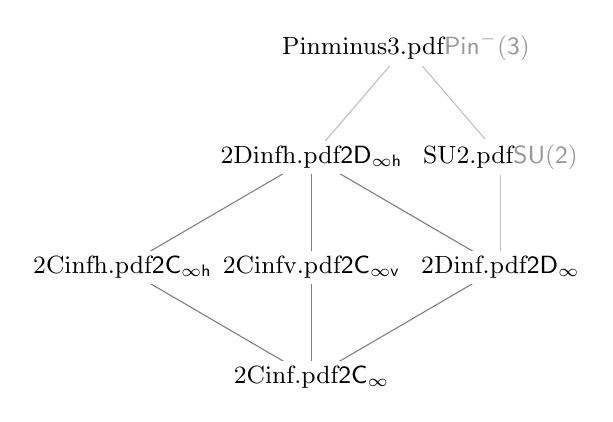
\begin{tikzpicture}[x=1cm, y=1cm, every node/.style={fill=white, font=\small, inner sep=2pt}]
\draw[black!50, line width=0.4pt] (0,0) -- (-2.4,1.4);
\draw[black!50, line width=0.4pt] (0,0) -- (0,1.4);
\draw[black!50, line width=0.4pt] (0,0) -- (2.4,1.4);
\draw[black!50, line width=0.4pt] (-2.4,1.4) -- (0,2.8);
\draw[black!50, line width=0.4pt] (0,1.4) -- (0,2.8);
\draw[black!50, line width=0.4pt] (2.4,1.4) -- (0,2.8);
\draw[black!25, line width=0.4pt] (2.4,1.4) -- (2.4,2.8);
\draw[black!25, line width=0.4pt] (0,2.8) -- (1.2,4.2);
\draw[black!25, line width=0.4pt] (2.4,2.8) -- (1.2,4.2);
\node at (0,0) {\href{2Cinf.pdf}{\textcolor{black}{$\grp{2C_{\infty }}$}}};
\node at (-2.4,1.4) {\href{2Cinfh.pdf}{\textcolor{black}{$\grp{2C_{\infty h}}$}}};
\node at (0,1.4) {\href{2Cinfv.pdf}{\textcolor{black}{$\grp{2C_{\infty v}}$}}};
\node at (2.4,1.4) {\href{2Dinf.pdf}{\textcolor{black}{$\grp{2D_{\infty }}$}}};
\node at (0,2.8) {\href{2Dinfh.pdf}{\textcolor{black}{$\grp{2D_{\infty h}}$}}};
\node at (2.4,2.8) {\href{SU2.pdf}{\textcolor{black!40}{$\grp{SU(2)}$}}};
\node at (1.2,4.2) {\href{Pinminus3.pdf}{\textcolor{black!40}{$\grp{Pin^{-}(3)}$}}};
\end{tikzpicture}\end{center}
\leavevmode\label{n:group.H}The table lists the closed subgroups $\grp{H}$ other than $\grp{2D_{\infty h}}$ up to conjugacy in $\grp{2D_{\infty h}}$, one in each row: the continuous subgroups, then the preimages and the sections of each family. Members of different families are not conjugate in $\grp{2D_{\infty h}}$, also where they lie in one \href{Pinminus3.pdf}{$\grp{Pin^{-}(3)}$}-conjugacy class. A row with $N$ in its symbol stands for every $N$ of its range, and its entries are functions of $N$. \label{n:head.subgroup}\label{n:head.order}\label{n:head.conjugates}\label{n:head.normal}A row gives the representative $\grp{H}$ of a class of subgroups (subgrp), its order, the number of subgroups in the class (conjugates) and whether $\grp{H}$ is normal. \label{n:group.normalizer}\label{n:group.centralizer}It also gives the normalizer $\grp{N}_{\hairsp \grp{2D_{\infty h}}}(\grp{H})$ and the centralizer $\grp{C}_{\hairsp \grp{2D_{\infty h}}}(\grp{H})$ in $\grp{2D_{\infty h}}$ (\texttt{normalizer}, \texttt{centralizer}). \label{n:head.components}The column components gives the components of the class space (section~\ref{s:class_space}) met by the subgroup. The record holds the members with $N \le 12$ (\texttt{subduction\symbol{95}subgroups}). A subgroup's other names in its \href{Pinminus3.pdf}{$\grp{Pin^{-}(3)}$}-conjugacy class follow $\samecls$ (\href{../../CONVENTIONS.pdf}{CONVENTIONS.pdf}, section \href{../../CONVENTIONS.pdf\#conv.20.2}{20.2}).
{\small\setlength{\fillwidth}{\textwidth}\addtolength{\fillwidth}{-12\tabcolsep}\setlength{\colwidth}{0pt}\cellmax{$\grp{S_{2\mathnormal{N}}}\secondclass$, $N \ge 3$ odd}\cellmax{$\grp{2C_{1h}}$ $\samecls$ $\grp{2C_{1v}}$}\cellmax{$\grp{2C_{2h}}$ $\samecls$ $\grp{2D_{1d}}$}\cellmax{$\grp{2C_{2v}}$ $\samecls$ $\grp{2D_{1h}}$}\cellmax{$\grp{2D_{1d}}$ $\samecls$ $\grp{2C_{2h}}$}\cellmax{$\grp{2D_{1h}}$ $\samecls$ $\grp{2C_{2v}}$}\cellmax{$\grp{S_{2\mathnormal{N}}}$, $N \ge 3$ odd}\cellmax{$\grp{2C_{s}}$ $\samecls$ $\grp{2C_{1h}}$}\cellmax{$\grp{C_{\mathnormal{N}}}$, $N \ge 3$ odd}\cellmax{$\grp{2C_{2}}$ $\samecls$ $\grp{2D_{1}}$}\cellmax{$\grp{2C_{\mathnormal{N}h}}$, $N \ge 3$}\cellmax{$\grp{2C_{\mathnormal{N}v}}$, $N \ge 3$}\cellmax{$\grp{2D_{1}}$ $\samecls$ $\grp{2C_{2}}$}\cellmax{$\grp{2D_{\mathnormal{N}d}}$, $N \ge 2$}\cellmax{$\grp{2D_{\mathnormal{N}h}}$, $N \ge 2$}\cellmax{$\grp{2S_{2\mathnormal{N}}}$, $N \ge 2$}\cellmax{$\grp{2C_{\mathnormal{N}}}$, $N \ge 3$}\cellmax{$\grp{2D_{\mathnormal{N}}}$, $N \ge 2$}\cellmax{subgrp}\cellmax{$\grp{2C_{\infty h}}$}\cellmax{$\grp{2C_{\infty v}}$}\cellmax{$\grp{2C_{1}}$}\cellmax{$\grp{2C_{\infty }}$}\cellmax{$\grp{2C_{i}}$}\cellmax{$\grp{2D_{\infty }}$}\cellmax{$\grp{C_{i}}\secondclass$}\cellmax{$\grp{C_{1}}$}\cellmax{$\grp{C_{i}}$}\addtolength{\fillwidth}{-\colwidth}\setlength{\colwidth}{0pt}\cellmax{order}\cellmax{$2N$}\cellmax{$4N$}\cellmax{$8N$}\cellmax{$N$}\cellmax{$\infty$}\cellmax{1}\cellmax{2}\cellmax{4}\cellmax{8}\addtolength{\fillwidth}{-\colwidth}\setlength{\colwidth}{0pt}\cellmax{conjugates}\cellmax{$\infty$}\cellmax{1}\addtolength{\fillwidth}{-\colwidth}\setlength{\colwidth}{0pt}\cellmax{normal}\cellmax{yes}\cellmax{no}\addtolength{\fillwidth}{-\colwidth}\setlength{\colwidth}{0pt}\cellmax{$\grp{N}_{\hairsp \grp{2D_{\infty h}}}(\grp{H})$}\cellmax{$\grp{2D_{2\mathnormal{N}h}}$}\cellmax{$\grp{2D_{2h}}$}\cellmax{$\grp{2D_{4h}}$}\cellmax{$\grp{2D_{\infty h}}$}\addtolength{\fillwidth}{-\colwidth}\setlength{\colwidth}{0pt}\cellmax{$\grp{C}_{\hairsp \grp{2D_{\infty h}}}(\grp{H})$}\cellmax{$\grp{2C_{2h}}$}\cellmax{$\grp{2C_{\infty h}}$}\cellmax{$\grp{2D_{\infty h}}$}\cellmax{$\grp{2C_{i}}$}\addtolength{\fillwidth}{-\colwidth}\setlength{\colwidth}{0pt}\cellmax{$\comp{\lift{C}(\omega)}$, $\comp{\infty\lift{C}_2'}$, $\comp{\lift{i}\,\lift{C}(\omega)}$, $\comp{\infty\lift{\sigma}_v}$}\cellmax{$\comp{\lift{C}(\omega)}$, $\comp{\lift{i}\,\lift{C}(\omega)}$}\cellmax{$\comp{\lift{C}(\omega)}$, $\comp{\infty\lift{C}_2'}$}\cellmax{$\comp{\lift{C}(\omega)}$, $\comp{\infty\lift{\sigma}_v}$}\cellmax{components}\cellmax{$\comp{\lift{C}(\omega)}$}\fillcap\begin{longtable}{@{}lrrlll>{\RaggedRight\arraybackslash}p{\fillwidth}@{}}\toprule
subgrp & order & conjugates & normal & $\grp{N}_{\hairsp \grp{2D_{\infty h}}}(\grp{H})$ & $\grp{C}_{\hairsp \grp{2D_{\infty h}}}(\grp{H})$ & components\\\midrule\endhead
\bottomrule\endfoot\endlastfoot
\href{2Cinf.pdf}{$\grp{2C_{\infty }}$} & $\infty$ & 1 & yes & \href{2Dinfh.pdf}{$\grp{2D_{\infty h}}$} & \href{2Cinfh.pdf}{$\grp{2C_{\infty h}}$} & $\comp{\lift{C}(\omega)}$\\*
\href{2Cinfh.pdf}{$\grp{2C_{\infty h}}$} & $\infty$ & 1 & yes & \href{2Dinfh.pdf}{$\grp{2D_{\infty h}}$} & \href{2Cinfh.pdf}{$\grp{2C_{\infty h}}$} & $\comp{\lift{C}(\omega)}$, $\comp{\lift{i}\,\lift{C}(\omega)}$\\
\href{2Cinfv.pdf}{$\grp{2C_{\infty v}}$} & $\infty$ & 1 & yes & \href{2Dinfh.pdf}{$\grp{2D_{\infty h}}$} & \href{2S2.pdf}{$\grp{2C_{i}}$} & $\comp{\lift{C}(\omega)}$, $\comp{\infty\lift{\sigma}_v}$\\
\href{2Dinf.pdf}{$\grp{2D_{\infty }}$} & $\infty$ & 1 & yes & \href{2Dinfh.pdf}{$\grp{2D_{\infty h}}$} & \href{2S2.pdf}{$\grp{2C_{i}}$} & $\comp{\lift{C}(\omega)}$, $\comp{\infty\lift{C}_2'}$\\
\grouprule{0pt}{\lightrulewidth}
\href{2C1.pdf}{$\grp{2C_{1}}$} & 2 & 1 & yes & \href{2Dinfh.pdf}{$\grp{2D_{\infty h}}$} & \href{2Dinfh.pdf}{$\grp{2D_{\infty h}}$} & $\comp{\lift{C}(\omega)}$\\
\href{2C2.pdf}{$\grp{2C_{2}}$} $\samecls$ \href{2D1.pdf}{$\grp{2D_{1}}$} & 4 & 1 & yes & \href{2Dinfh.pdf}{$\grp{2D_{\infty h}}$} & \href{2Cinfh.pdf}{$\grp{2C_{\infty h}}$} & $\comp{\lift{C}(\omega)}$\\
$\grp{2C_{\mathnormal{N}}}$, $N \ge 3$ & $2N$ & 1 & yes & \href{2Dinfh.pdf}{$\grp{2D_{\infty h}}$} & \href{2Cinfh.pdf}{$\grp{2C_{\infty h}}$} & $\comp{\lift{C}(\omega)}$\\
\href{C1.pdf}{$\grp{C_{1}}$} & 1 & 1 & yes & \href{2Dinfh.pdf}{$\grp{2D_{\infty h}}$} & \href{2Dinfh.pdf}{$\grp{2D_{\infty h}}$} & $\comp{\lift{C}(\omega)}$\\
$\grp{C_{\mathnormal{N}}}$, $N \ge 3$ odd & $N$ & 1 & yes & \href{2Dinfh.pdf}{$\grp{2D_{\infty h}}$} & \href{2Cinfh.pdf}{$\grp{2C_{\infty h}}$} & $\comp{\lift{C}(\omega)}$\\
\grouprule{0pt}{\lightrulewidth}
\href{2S2.pdf}{$\grp{2C_{i}}$} & 4 & 1 & yes & \href{2Dinfh.pdf}{$\grp{2D_{\infty h}}$} & \href{2Dinfh.pdf}{$\grp{2D_{\infty h}}$} & $\comp{\lift{C}(\omega)}$, $\comp{\lift{i}\,\lift{C}(\omega)}$\\
$\grp{2S_{2\mathnormal{N}}}$, $N \ge 2$ & $4N$ & 1 & yes & \href{2Dinfh.pdf}{$\grp{2D_{\infty h}}$} & \href{2Cinfh.pdf}{$\grp{2C_{\infty h}}$} & $\comp{\lift{C}(\omega)}$, $\comp{\lift{i}\,\lift{C}(\omega)}$\\
\href{S2.pdf}{$\grp{C_{i}}$} & 2 & 1 & yes & \href{2Dinfh.pdf}{$\grp{2D_{\infty h}}$} & \href{2Dinfh.pdf}{$\grp{2D_{\infty h}}$} & $\comp{\lift{C}(\omega)}$, $\comp{\lift{i}\,\lift{C}(\omega)}$\\
$\grp{S_{2\mathnormal{N}}}$, $N \ge 3$ odd & $2N$ & 1 & yes & \href{2Dinfh.pdf}{$\grp{2D_{\infty h}}$} & \href{2Cinfh.pdf}{$\grp{2C_{\infty h}}$} & $\comp{\lift{C}(\omega)}$, $\comp{\lift{i}\,\lift{C}(\omega)}$\\
\href{S2b.pdf}{$\grp{C_{i}}\secondclass$} & 2 & 1 & yes & \href{2Dinfh.pdf}{$\grp{2D_{\infty h}}$} & \href{2Dinfh.pdf}{$\grp{2D_{\infty h}}$} & $\comp{\lift{C}(\omega)}$, $\comp{\lift{i}\,\lift{C}(\omega)}$\\
$\grp{S_{2\mathnormal{N}}}\secondclass$, $N \ge 3$ odd & $2N$ & 1 & yes & \href{2Dinfh.pdf}{$\grp{2D_{\infty h}}$} & \href{2Cinfh.pdf}{$\grp{2C_{\infty h}}$} & $\comp{\lift{C}(\omega)}$, $\comp{\lift{i}\,\lift{C}(\omega)}$\\
\grouprule{0pt}{\lightrulewidth}
\href{2C1h.pdf}{$\grp{2C_{1h}}$} $\samecls$ \href{2C1v.pdf}{$\grp{2C_{1v}}$} & 4 & 1 & yes & \href{2Dinfh.pdf}{$\grp{2D_{\infty h}}$} & \href{2Cinfh.pdf}{$\grp{2C_{\infty h}}$} & $\comp{\lift{C}(\omega)}$, $\comp{\lift{i}\,\lift{C}(\omega)}$\\
\href{2C2h.pdf}{$\grp{2C_{2h}}$} $\samecls$ \href{2D1d.pdf}{$\grp{2D_{1d}}$} & 8 & 1 & yes & \href{2Dinfh.pdf}{$\grp{2D_{\infty h}}$} & \href{2Cinfh.pdf}{$\grp{2C_{\infty h}}$} & $\comp{\lift{C}(\omega)}$, $\comp{\lift{i}\,\lift{C}(\omega)}$\\
$\grp{2C_{\mathnormal{N}h}}$, $N \ge 3$ & $4N$ & 1 & yes & \href{2Dinfh.pdf}{$\grp{2D_{\infty h}}$} & \href{2Cinfh.pdf}{$\grp{2C_{\infty h}}$} & $\comp{\lift{C}(\omega)}$, $\comp{\lift{i}\,\lift{C}(\omega)}$\\
\grouprule{0pt}{\lightrulewidth}
\href{2C1v.pdf}{$\grp{2C_{s}}$} $\samecls$ \href{2C1h.pdf}{$\grp{2C_{1h}}$} & 4 & $\infty$ & no & \href{2D2h.pdf}{$\grp{2D_{2h}}$} & \href{2C2h.pdf}{$\grp{2C_{2h}}$} & $\comp{\lift{C}(\omega)}$, $\comp{\infty\lift{\sigma}_v}$\\
\href{2C2v.pdf}{$\grp{2C_{2v}}$} $\samecls$ \href{2D1h.pdf}{$\grp{2D_{1h}}$} & 8 & $\infty$ & no & \href{2D4h.pdf}{$\grp{2D_{4h}}$} & \href{2S2.pdf}{$\grp{2C_{i}}$} & $\comp{\lift{C}(\omega)}$, $\comp{\infty\lift{\sigma}_v}$\\
$\grp{2C_{\mathnormal{N}v}}$, $N \ge 3$ & $4N$ & $\infty$ & no & $\grp{2D_{2\mathnormal{N}h}}$ & \href{2S2.pdf}{$\grp{2C_{i}}$} & $\comp{\lift{C}(\omega)}$, $\comp{\infty\lift{\sigma}_v}$\\
\grouprule{0pt}{\lightrulewidth}
\href{2D1.pdf}{$\grp{2D_{1}}$} $\samecls$ \href{2C2.pdf}{$\grp{2C_{2}}$} & 4 & $\infty$ & no & \href{2D2h.pdf}{$\grp{2D_{2h}}$} & \href{2C2h.pdf}{$\grp{2C_{2h}}$} & $\comp{\lift{C}(\omega)}$, $\comp{\infty\lift{C}_2'}$\\
$\grp{2D_{\mathnormal{N}}}$, $N \ge 2$ & $4N$ & $\infty$ & no & $\grp{2D_{2\mathnormal{N}h}}$ & \href{2S2.pdf}{$\grp{2C_{i}}$} & $\comp{\lift{C}(\omega)}$, $\comp{\infty\lift{C}_2'}$\\
\grouprule{0pt}{\lightrulewidth}
\href{2D1h.pdf}{$\grp{2D_{1h}}$} $\samecls$ \href{2C2v.pdf}{$\grp{2C_{2v}}$} & 8 & $\infty$ & no & \href{2D2h.pdf}{$\grp{2D_{2h}}$} & \href{2S2.pdf}{$\grp{2C_{i}}$} & $\comp{\lift{C}(\omega)}$, $\comp{\infty\lift{C}_2'}$, $\comp{\lift{i}\,\lift{C}(\omega)}$, $\comp{\infty\lift{\sigma}_v}$\\
$\grp{2D_{\mathnormal{N}h}}$, $N \ge 2$ & $8N$ & $\infty$ & no & $\grp{2D_{2\mathnormal{N}h}}$ & \href{2S2.pdf}{$\grp{2C_{i}}$} & $\comp{\lift{C}(\omega)}$, $\comp{\infty\lift{C}_2'}$, $\comp{\lift{i}\,\lift{C}(\omega)}$, $\comp{\infty\lift{\sigma}_v}$\\
\grouprule{0pt}{\lightrulewidth}
\href{2D1d.pdf}{$\grp{2D_{1d}}$} $\samecls$ \href{2C2h.pdf}{$\grp{2C_{2h}}$} & 8 & $\infty$ & no & \href{2D2h.pdf}{$\grp{2D_{2h}}$} & \href{2C2h.pdf}{$\grp{2C_{2h}}$} & $\comp{\lift{C}(\omega)}$, $\comp{\infty\lift{C}_2'}$, $\comp{\lift{i}\,\lift{C}(\omega)}$, $\comp{\infty\lift{\sigma}_v}$\\*
$\grp{2D_{\mathnormal{N}d}}$, $N \ge 2$ & $8N$ & $\infty$ & no & $\grp{2D_{2\mathnormal{N}h}}$ & \href{2S2.pdf}{$\grp{2C_{i}}$} & $\comp{\lift{C}(\omega)}$, $\comp{\infty\lift{C}_2'}$, $\comp{\lift{i}\,\lift{C}(\omega)}$, $\comp{\infty\lift{\sigma}_v}$\\
\bottomrule\end{longtable}}
\needspace{203pt}
\section{Descent of symmetry}\label{s:subduction}
Conventions: \href{../../CONVENTIONS.pdf}{CONVENTIONS.pdf}, sections \href{../../../rotation/CONVENTIONS.pdf\#conv.16.1}{16.1} and \href{../../CONVENTIONS.pdf\#conv.29.5}{29.5}.
\needspace{149pt}
\paragraph{Vector families.} The vector families of $\grp{2D_{\infty h}}$ are those of \href{../../../rotation/data/pdf/Dinfh.pdf}{$\grp{D_{\infty h}}$}. They restrict to the preimage $\grp{2H}$ of a closed subgroup $\grp{H}$ of \href{../../../rotation/data/pdf/Dinfh.pdf}{$\grp{D_{\infty h}}$} as \href{../../../rotation/data/pdf/Dinfh.pdf}{$\grp{D_{\infty h}}$} restricts them to $\grp{H}$ (\texttt{vector\symbol{95}entry}, \texttt{vector\symbol{95}rules}), whose irreps are the vector irreps of $\grp{2H}$. The families restrict to a section as to its preimage. The tables are those of the section Descent of symmetry of the document of \href{../../../rotation/data/pdf/Dinfh.pdf}{$\grp{D_{\infty h}}$}, with its settings. They are headed by the preimages and give the images of the generators of $\grp{H}$ at the points of the class space (section~\ref{s:class_space}). Members of different families are not conjugate in $\grp{2D_{\infty h}}$, also where they lie in one \href{Pinminus3.pdf}{$\grp{Pin^{-}(3)}$}-conjugacy class, such as \href{2D1.pdf}{$\grp{2D_{1}}$} and \href{2C2.pdf}{$\grp{2C_{2}}$} (a binary axis perpendicular to $z$ and along $z$). \label{n:irrep.Gamma.subgroup}The entry of row $\Gamma$ is $\restr{\Gamma}{\grp{H}}$ as a sum of the irreps of $\grp{H}$.
{\small\begin{longtable}{@{}lcccc@{}}\toprule
subgrp & \href{2Cinf.pdf}{$\grp{2C_{\infty }}$} & \href{2Cinfh.pdf}{$\grp{2C_{\infty h}}$} & \href{2Cinfv.pdf}{$\grp{2C_{\infty v}}$} & \href{2Dinf.pdf}{$\grp{2D_{\infty }}$}\\
index & 4 & 2 & 2 & 2\\\midrule\endhead
\bottomrule\endfoot\endlastfoot
$\irr{a}_{1\ptag{g}}$ & $\irr{a}$ & $\irr{a}_{\ptag{g}}$ & $\irr{a}_{1}$ & $\irr{a}_{1}$\\*
$\irr{a}_{2\ptag{g}}$ & $\irr{a}$ & $\irr{a}_{\ptag{g}}$ & $\irr{a}_{2}$ & $\irr{a}_{2}$\\*
$\irr{e}_{n,\ptag{g}}$ & $\conjpair{1}\irr{e}_{n}\oplus \conjpair{2}\irr{e}_{n}$ & $\conjpair{1}\irr{e}_{n,\ptag{g}}\oplus \conjpair{2}\irr{e}_{n,\ptag{g}}$ & $\irr{e}_{n}$ & $\irr{e}_{n}$\\*
$\irr{a}_{1\ptag{u}}$ & $\irr{a}$ & $\irr{a}_{\ptag{u}}$ & $\irr{a}_{2}$ & $\irr{a}_{1}$\\*
$\irr{a}_{2\ptag{u}}$ & $\irr{a}$ & $\irr{a}_{\ptag{u}}$ & $\irr{a}_{1}$ & $\irr{a}_{2}$\\*
$\irr{e}_{n,\ptag{u}}$ & $\conjpair{1}\irr{e}_{n}\oplus \conjpair{2}\irr{e}_{n}$ & $\conjpair{1}\irr{e}_{n,\ptag{u}}\oplus \conjpair{2}\irr{e}_{n,\ptag{u}}$ & $\irr{e}_{n}$ & $\irr{e}_{n}$\\
\bottomrule\end{longtable}}

\needspace{95pt}
\paragraph{Vector families, the $\grp{2C_{\mathnormal{N}}}$ family.}
{\small\setlength{\fillwidth}{\textwidth}\addtolength{\fillwidth}{-2\tabcolsep}\setlength{\colwidth}{0pt}\cellmax{$\irr{e}_{n,\ptag{g}}$}\cellmax{$\irr{e}_{n,\ptag{u}}$}\cellmax{$\irr{a}_{1\ptag{g}}$}\cellmax{$\irr{a}_{1\ptag{u}}$}\cellmax{$\irr{a}_{2\ptag{g}}$}\cellmax{$\irr{a}_{2\ptag{u}}$}\addtolength{\fillwidth}{-\colwidth}\setlength{\colwidth}{0pt}\cellmax{$2\,\irr{a}$ if $q = 0$, $2\,\irr{b}$ if $q = N/2$, $\conjpair{1}\irr{e}_{\min(q, N-q)}\oplus \conjpair{2}\irr{e}_{\min(q, N-q)}$ otherwise; $q = n \bmod N$}\cellmax{$\irr{a}$}\fillcap\begin{longtable}{@{}l>{\raggedright\arraybackslash}p{\fillwidth}@{}}\toprule
\multicolumn{2}{@{}c@{}}{every $N$}\\*
$\irr{a}_{1\ptag{g}}$ & $\irr{a}$\\*
$\irr{a}_{2\ptag{g}}$ & $\irr{a}$\\*
$\irr{e}_{n,\ptag{g}}$ & $2\,\irr{a}$ if $q = 0$, $2\,\irr{b}$ if $q = N/2$, $\conjpair{1}\irr{e}_{\min(q, N-q)}\oplus \conjpair{2}\irr{e}_{\min(q, N-q)}$ otherwise; $q = n \bmod N$\\*
$\irr{a}_{1\ptag{u}}$ & $\irr{a}$\\*
$\irr{a}_{2\ptag{u}}$ & $\irr{a}$\\*
$\irr{e}_{n,\ptag{u}}$ & $2\,\irr{a}$ if $q = 0$, $2\,\irr{b}$ if $q = N/2$, $\conjpair{1}\irr{e}_{\min(q, N-q)}\oplus \conjpair{2}\irr{e}_{\min(q, N-q)}$ otherwise; $q = n \bmod N$\\
\bottomrule\end{longtable}}
{\small\begin{longtable}{@{}lcccccccc@{}}\toprule
subgrp & \href{2C2.pdf}{$\grp{2C_{2}}$} & \href{2C3.pdf}{$\grp{2C_{3}}$} & \href{2C4.pdf}{$\grp{2C_{4}}$} & \href{2C5.pdf}{$\grp{2C_{5}}$} & \href{2C6.pdf}{$\grp{2C_{6}}$} & \href{2C7.pdf}{$\grp{2C_{7}}$} & \href{2C8.pdf}{$\grp{2C_{8}}$} & \href{2C9.pdf}{$\grp{2C_{9}}$}\\\midrule\endhead
\bottomrule\endfoot\endlastfoot
$\irr{a}_{1\ptag{g}}$ & $\irr{a}$ & $\irr{a}$ & $\irr{a}$ & $\irr{a}$ & $\irr{a}$ & $\irr{a}$ & $\irr{a}$ & $\irr{a}$\\*
$\irr{a}_{2\ptag{g}}$ & $\irr{a}$ & $\irr{a}$ & $\irr{a}$ & $\irr{a}$ & $\irr{a}$ & $\irr{a}$ & $\irr{a}$ & $\irr{a}$\\
$\irr{e}_{1\ptag{g}}$ & $2\,\irr{b}$ & $\conjpair{1}\irr{e}\oplus \conjpair{2}\irr{e}$ & $\conjpair{1}\irr{e}\oplus \conjpair{2}\irr{e}$ & $\conjpair{1}\irr{e}_{1}\oplus \conjpair{2}\irr{e}_{1}$ & $\conjpair{1}\irr{e}_{1}\oplus \conjpair{2}\irr{e}_{1}$ & $\conjpair{1}\irr{e}_{1}\oplus \conjpair{2}\irr{e}_{1}$ & $\conjpair{1}\irr{e}_{1}\oplus \conjpair{2}\irr{e}_{1}$ & $\conjpair{1}\irr{e}_{1}\oplus \conjpair{2}\irr{e}_{1}$\\
$\irr{e}_{2\ptag{g}}$ & $2\,\irr{a}$ & $\conjpair{1}\irr{e}\oplus \conjpair{2}\irr{e}$ & $2\,\irr{b}$ & $\conjpair{1}\irr{e}_{2}\oplus \conjpair{2}\irr{e}_{2}$ & $\conjpair{1}\irr{e}_{2}\oplus \conjpair{2}\irr{e}_{2}$ & $\conjpair{1}\irr{e}_{2}\oplus \conjpair{2}\irr{e}_{2}$ & $\conjpair{1}\irr{e}_{2}\oplus \conjpair{2}\irr{e}_{2}$ & $\conjpair{1}\irr{e}_{2}\oplus \conjpair{2}\irr{e}_{2}$\\
$\irr{e}_{3\ptag{g}}$ & $2\,\irr{b}$ & $2\,\irr{a}$ & $\conjpair{1}\irr{e}\oplus \conjpair{2}\irr{e}$ & $\conjpair{1}\irr{e}_{2}\oplus \conjpair{2}\irr{e}_{2}$ & $2\,\irr{b}$ & $\conjpair{1}\irr{e}_{3}\oplus \conjpair{2}\irr{e}_{3}$ & $\conjpair{1}\irr{e}_{3}\oplus \conjpair{2}\irr{e}_{3}$ & $\conjpair{1}\irr{e}_{3}\oplus \conjpair{2}\irr{e}_{3}$\\
$\irr{e}_{4\ptag{g}}$ & $2\,\irr{a}$ & $\conjpair{1}\irr{e}\oplus \conjpair{2}\irr{e}$ & $2\,\irr{a}$ & $\conjpair{1}\irr{e}_{1}\oplus \conjpair{2}\irr{e}_{1}$ & $\conjpair{1}\irr{e}_{2}\oplus \conjpair{2}\irr{e}_{2}$ & $\conjpair{1}\irr{e}_{3}\oplus \conjpair{2}\irr{e}_{3}$ & $2\,\irr{b}$ & $\conjpair{1}\irr{e}_{4}\oplus \conjpair{2}\irr{e}_{4}$\\
$\irr{e}_{5\ptag{g}}$ & $2\,\irr{b}$ & $\conjpair{1}\irr{e}\oplus \conjpair{2}\irr{e}$ & $\conjpair{1}\irr{e}\oplus \conjpair{2}\irr{e}$ & $2\,\irr{a}$ & $\conjpair{1}\irr{e}_{1}\oplus \conjpair{2}\irr{e}_{1}$ & $\conjpair{1}\irr{e}_{2}\oplus \conjpair{2}\irr{e}_{2}$ & $\conjpair{1}\irr{e}_{3}\oplus \conjpair{2}\irr{e}_{3}$ & $\conjpair{1}\irr{e}_{4}\oplus \conjpair{2}\irr{e}_{4}$\\
$\irr{e}_{6\ptag{g}}$ & $2\,\irr{a}$ & $2\,\irr{a}$ & $2\,\irr{b}$ & $\conjpair{1}\irr{e}_{1}\oplus \conjpair{2}\irr{e}_{1}$ & $2\,\irr{a}$ & $\conjpair{1}\irr{e}_{1}\oplus \conjpair{2}\irr{e}_{1}$ & $\conjpair{1}\irr{e}_{2}\oplus \conjpair{2}\irr{e}_{2}$ & $\conjpair{1}\irr{e}_{3}\oplus \conjpair{2}\irr{e}_{3}$\\
$\irr{a}_{1\ptag{u}}$ & $\irr{a}$ & $\irr{a}$ & $\irr{a}$ & $\irr{a}$ & $\irr{a}$ & $\irr{a}$ & $\irr{a}$ & $\irr{a}$\\
$\irr{a}_{2\ptag{u}}$ & $\irr{a}$ & $\irr{a}$ & $\irr{a}$ & $\irr{a}$ & $\irr{a}$ & $\irr{a}$ & $\irr{a}$ & $\irr{a}$\\
$\irr{e}_{1\ptag{u}}$ & $2\,\irr{b}$ & $\conjpair{1}\irr{e}\oplus \conjpair{2}\irr{e}$ & $\conjpair{1}\irr{e}\oplus \conjpair{2}\irr{e}$ & $\conjpair{1}\irr{e}_{1}\oplus \conjpair{2}\irr{e}_{1}$ & $\conjpair{1}\irr{e}_{1}\oplus \conjpair{2}\irr{e}_{1}$ & $\conjpair{1}\irr{e}_{1}\oplus \conjpair{2}\irr{e}_{1}$ & $\conjpair{1}\irr{e}_{1}\oplus \conjpair{2}\irr{e}_{1}$ & $\conjpair{1}\irr{e}_{1}\oplus \conjpair{2}\irr{e}_{1}$\\
$\irr{e}_{2\ptag{u}}$ & $2\,\irr{a}$ & $\conjpair{1}\irr{e}\oplus \conjpair{2}\irr{e}$ & $2\,\irr{b}$ & $\conjpair{1}\irr{e}_{2}\oplus \conjpair{2}\irr{e}_{2}$ & $\conjpair{1}\irr{e}_{2}\oplus \conjpair{2}\irr{e}_{2}$ & $\conjpair{1}\irr{e}_{2}\oplus \conjpair{2}\irr{e}_{2}$ & $\conjpair{1}\irr{e}_{2}\oplus \conjpair{2}\irr{e}_{2}$ & $\conjpair{1}\irr{e}_{2}\oplus \conjpair{2}\irr{e}_{2}$\\
$\irr{e}_{3\ptag{u}}$ & $2\,\irr{b}$ & $2\,\irr{a}$ & $\conjpair{1}\irr{e}\oplus \conjpair{2}\irr{e}$ & $\conjpair{1}\irr{e}_{2}\oplus \conjpair{2}\irr{e}_{2}$ & $2\,\irr{b}$ & $\conjpair{1}\irr{e}_{3}\oplus \conjpair{2}\irr{e}_{3}$ & $\conjpair{1}\irr{e}_{3}\oplus \conjpair{2}\irr{e}_{3}$ & $\conjpair{1}\irr{e}_{3}\oplus \conjpair{2}\irr{e}_{3}$\\
$\irr{e}_{4\ptag{u}}$ & $2\,\irr{a}$ & $\conjpair{1}\irr{e}\oplus \conjpair{2}\irr{e}$ & $2\,\irr{a}$ & $\conjpair{1}\irr{e}_{1}\oplus \conjpair{2}\irr{e}_{1}$ & $\conjpair{1}\irr{e}_{2}\oplus \conjpair{2}\irr{e}_{2}$ & $\conjpair{1}\irr{e}_{3}\oplus \conjpair{2}\irr{e}_{3}$ & $2\,\irr{b}$ & $\conjpair{1}\irr{e}_{4}\oplus \conjpair{2}\irr{e}_{4}$\\
$\irr{e}_{5\ptag{u}}$ & $2\,\irr{b}$ & $\conjpair{1}\irr{e}\oplus \conjpair{2}\irr{e}$ & $\conjpair{1}\irr{e}\oplus \conjpair{2}\irr{e}$ & $2\,\irr{a}$ & $\conjpair{1}\irr{e}_{1}\oplus \conjpair{2}\irr{e}_{1}$ & $\conjpair{1}\irr{e}_{2}\oplus \conjpair{2}\irr{e}_{2}$ & $\conjpair{1}\irr{e}_{3}\oplus \conjpair{2}\irr{e}_{3}$ & $\conjpair{1}\irr{e}_{4}\oplus \conjpair{2}\irr{e}_{4}$\\*
$\irr{e}_{6\ptag{u}}$ & $2\,\irr{a}$ & $2\,\irr{a}$ & $2\,\irr{b}$ & $\conjpair{1}\irr{e}_{1}\oplus \conjpair{2}\irr{e}_{1}$ & $2\,\irr{a}$ & $\conjpair{1}\irr{e}_{1}\oplus \conjpair{2}\irr{e}_{1}$ & $\conjpair{1}\irr{e}_{2}\oplus \conjpair{2}\irr{e}_{2}$ & $\conjpair{1}\irr{e}_{3}\oplus \conjpair{2}\irr{e}_{3}$\\
\bottomrule\end{longtable}}
{\small\begin{longtable}{@{}lccc@{}}\toprule
subgrp & \href{2C10.pdf}{$\grp{2C_{10}}$} & \href{2C11.pdf}{$\grp{2C_{11}}$} & \href{2C12.pdf}{$\grp{2C_{12}}$}\\\midrule\endhead
\bottomrule\endfoot\endlastfoot
$\irr{a}_{1\ptag{g}}$ & $\irr{a}$ & $\irr{a}$ & $\irr{a}$\\*
$\irr{a}_{2\ptag{g}}$ & $\irr{a}$ & $\irr{a}$ & $\irr{a}$\\
$\irr{e}_{1\ptag{g}}$ & $\conjpair{1}\irr{e}_{1}\oplus \conjpair{2}\irr{e}_{1}$ & $\conjpair{1}\irr{e}_{1}\oplus \conjpair{2}\irr{e}_{1}$ & $\conjpair{1}\irr{e}_{1}\oplus \conjpair{2}\irr{e}_{1}$\\
$\irr{e}_{2\ptag{g}}$ & $\conjpair{1}\irr{e}_{2}\oplus \conjpair{2}\irr{e}_{2}$ & $\conjpair{1}\irr{e}_{2}\oplus \conjpair{2}\irr{e}_{2}$ & $\conjpair{1}\irr{e}_{2}\oplus \conjpair{2}\irr{e}_{2}$\\
$\irr{e}_{3\ptag{g}}$ & $\conjpair{1}\irr{e}_{3}\oplus \conjpair{2}\irr{e}_{3}$ & $\conjpair{1}\irr{e}_{3}\oplus \conjpair{2}\irr{e}_{3}$ & $\conjpair{1}\irr{e}_{3}\oplus \conjpair{2}\irr{e}_{3}$\\
$\irr{e}_{4\ptag{g}}$ & $\conjpair{1}\irr{e}_{4}\oplus \conjpair{2}\irr{e}_{4}$ & $\conjpair{1}\irr{e}_{4}\oplus \conjpair{2}\irr{e}_{4}$ & $\conjpair{1}\irr{e}_{4}\oplus \conjpair{2}\irr{e}_{4}$\\
$\irr{e}_{5\ptag{g}}$ & $2\,\irr{b}$ & $\conjpair{1}\irr{e}_{5}\oplus \conjpair{2}\irr{e}_{5}$ & $\conjpair{1}\irr{e}_{5}\oplus \conjpair{2}\irr{e}_{5}$\\
$\irr{e}_{6\ptag{g}}$ & $\conjpair{1}\irr{e}_{4}\oplus \conjpair{2}\irr{e}_{4}$ & $\conjpair{1}\irr{e}_{5}\oplus \conjpair{2}\irr{e}_{5}$ & $2\,\irr{b}$\\
$\irr{a}_{1\ptag{u}}$ & $\irr{a}$ & $\irr{a}$ & $\irr{a}$\\
$\irr{a}_{2\ptag{u}}$ & $\irr{a}$ & $\irr{a}$ & $\irr{a}$\\
$\irr{e}_{1\ptag{u}}$ & $\conjpair{1}\irr{e}_{1}\oplus \conjpair{2}\irr{e}_{1}$ & $\conjpair{1}\irr{e}_{1}\oplus \conjpair{2}\irr{e}_{1}$ & $\conjpair{1}\irr{e}_{1}\oplus \conjpair{2}\irr{e}_{1}$\\
$\irr{e}_{2\ptag{u}}$ & $\conjpair{1}\irr{e}_{2}\oplus \conjpair{2}\irr{e}_{2}$ & $\conjpair{1}\irr{e}_{2}\oplus \conjpair{2}\irr{e}_{2}$ & $\conjpair{1}\irr{e}_{2}\oplus \conjpair{2}\irr{e}_{2}$\\
$\irr{e}_{3\ptag{u}}$ & $\conjpair{1}\irr{e}_{3}\oplus \conjpair{2}\irr{e}_{3}$ & $\conjpair{1}\irr{e}_{3}\oplus \conjpair{2}\irr{e}_{3}$ & $\conjpair{1}\irr{e}_{3}\oplus \conjpair{2}\irr{e}_{3}$\\
$\irr{e}_{4\ptag{u}}$ & $\conjpair{1}\irr{e}_{4}\oplus \conjpair{2}\irr{e}_{4}$ & $\conjpair{1}\irr{e}_{4}\oplus \conjpair{2}\irr{e}_{4}$ & $\conjpair{1}\irr{e}_{4}\oplus \conjpair{2}\irr{e}_{4}$\\
$\irr{e}_{5\ptag{u}}$ & $2\,\irr{b}$ & $\conjpair{1}\irr{e}_{5}\oplus \conjpair{2}\irr{e}_{5}$ & $\conjpair{1}\irr{e}_{5}\oplus \conjpair{2}\irr{e}_{5}$\\*
$\irr{e}_{6\ptag{u}}$ & $\conjpair{1}\irr{e}_{4}\oplus \conjpair{2}\irr{e}_{4}$ & $\conjpair{1}\irr{e}_{5}\oplus \conjpair{2}\irr{e}_{5}$ & $2\,\irr{b}$\\
\bottomrule\end{longtable}}

\needspace{95pt}
\paragraph{Vector families, the $\grp{2S_{2\mathnormal{N}}}$ family.}
{\small\setlength{\fillwidth}{\textwidth}\addtolength{\fillwidth}{-2\tabcolsep}\setlength{\colwidth}{0pt}\cellmax{$\irr{e}_{n,\ptag{g}}$}\cellmax{$\irr{e}_{n,\ptag{u}}$}\cellmax{$\irr{a}_{1\ptag{g}}$}\cellmax{$\irr{a}_{1\ptag{u}}$}\cellmax{$\irr{a}_{2\ptag{g}}$}\cellmax{$\irr{a}_{2\ptag{u}}$}\addtolength{\fillwidth}{-\colwidth}\setlength{\colwidth}{0pt}\cellmax{$2\,\irr{a}$ if $q = 0$, $2\,\irr{b}$ if $q = N$, $\conjpair{1}\irr{e}_{\min(q, 2N-q)}\oplus \conjpair{2}\irr{e}_{\min(q, 2N-q)}$ otherwise; $q = ((N+1)n + N) \bmod 2N$}\cellmax{$2\,\irr{a}$ if $q = 0$, $2\,\irr{b}$ if $q = N$, $\conjpair{1}\irr{e}_{\min(q, 2N-q)}\oplus \conjpair{2}\irr{e}_{\min(q, 2N-q)}$ otherwise; $q = (N+1)n \bmod 2N$}\cellmax{$2\,\irr{a}_{\ptag{g}}$ if $q = 0$, $\conjpair{1}\irr{e}_{\min(q, N-q),\ptag{g}}\oplus \conjpair{2}\irr{e}_{\min(q, N-q),\ptag{g}}$ otherwise; $q = n \bmod N$}\cellmax{$2\,\irr{a}_{\ptag{u}}$ if $q = 0$, $\conjpair{1}\irr{e}_{\min(q, N-q),\ptag{u}}\oplus \conjpair{2}\irr{e}_{\min(q, N-q),\ptag{u}}$ otherwise; $q = n \bmod N$}\cellmax{$\irr{a}_{\ptag{g}}$}\cellmax{$\irr{a}_{\ptag{u}}$}\cellmax{$\irr{a}$}\cellmax{$\irr{b}$}\fillcap\begin{longtable}{@{}l>{\raggedright\arraybackslash}p{\fillwidth}@{}}\toprule
\multicolumn{2}{@{}c@{}}{odd $N$}\\*
$\irr{a}_{1\ptag{g}}$ & $\irr{a}_{\ptag{g}}$\\*
$\irr{a}_{2\ptag{g}}$ & $\irr{a}_{\ptag{g}}$\\*
$\irr{e}_{n,\ptag{g}}$ & $2\,\irr{a}_{\ptag{g}}$ if $q = 0$, $\conjpair{1}\irr{e}_{\min(q, N-q),\ptag{g}}\oplus \conjpair{2}\irr{e}_{\min(q, N-q),\ptag{g}}$ otherwise; $q = n \bmod N$\\*
$\irr{a}_{1\ptag{u}}$ & $\irr{a}_{\ptag{u}}$\\*
$\irr{a}_{2\ptag{u}}$ & $\irr{a}_{\ptag{u}}$\\*
$\irr{e}_{n,\ptag{u}}$ & $2\,\irr{a}_{\ptag{u}}$ if $q = 0$, $\conjpair{1}\irr{e}_{\min(q, N-q),\ptag{u}}\oplus \conjpair{2}\irr{e}_{\min(q, N-q),\ptag{u}}$ otherwise; $q = n \bmod N$\\
\grouprule{0pt}{\lightrulewidth}
\multicolumn{2}{@{}c@{}}{even $N$}\\*
$\irr{a}_{1\ptag{g}}$ & $\irr{a}$\\*
$\irr{a}_{2\ptag{g}}$ & $\irr{a}$\\*
$\irr{e}_{n,\ptag{g}}$ & $2\,\irr{a}$ if $q = 0$, $2\,\irr{b}$ if $q = N$, $\conjpair{1}\irr{e}_{\min(q, 2N-q)}\oplus \conjpair{2}\irr{e}_{\min(q, 2N-q)}$ otherwise; $q = (N+1)n \bmod 2N$\\*
$\irr{a}_{1\ptag{u}}$ & $\irr{b}$\\*
$\irr{a}_{2\ptag{u}}$ & $\irr{b}$\\*
$\irr{e}_{n,\ptag{u}}$ & $2\,\irr{a}$ if $q = 0$, $2\,\irr{b}$ if $q = N$, $\conjpair{1}\irr{e}_{\min(q, 2N-q)}\oplus \conjpair{2}\irr{e}_{\min(q, 2N-q)}$ otherwise; $q = ((N+1)n + N) \bmod 2N$\\
\bottomrule\end{longtable}}
{\small\begin{longtable}{@{}lccccccc@{}}\toprule
subgrp & \href{2S2.pdf}{$\grp{2S_{2}}$} & \href{2S4.pdf}{$\grp{2S_{4}}$} & \href{2S6.pdf}{$\grp{2S_{6}}$} & \href{2S8.pdf}{$\grp{2S_{8}}$} & \href{2S10.pdf}{$\grp{2S_{10}}$} & \href{2S12.pdf}{$\grp{2S_{12}}$} & \href{2S14.pdf}{$\grp{2S_{14}}$}\\\midrule\endhead
\bottomrule\endfoot\endlastfoot
$\irr{a}_{1\ptag{g}}$ & $\irr{a}_{\ptag{g}}$ & $\irr{a}$ & $\irr{a}_{\ptag{g}}$ & $\irr{a}$ & $\irr{a}_{\ptag{g}}$ & $\irr{a}$ & $\irr{a}_{\ptag{g}}$\\*
$\irr{a}_{2\ptag{g}}$ & $\irr{a}_{\ptag{g}}$ & $\irr{a}$ & $\irr{a}_{\ptag{g}}$ & $\irr{a}$ & $\irr{a}_{\ptag{g}}$ & $\irr{a}$ & $\irr{a}_{\ptag{g}}$\\
$\irr{e}_{1\ptag{g}}$ & $2\,\irr{a}_{\ptag{g}}$ & $\conjpair{1}\irr{e}\oplus \conjpair{2}\irr{e}$ & $\conjpair{1}\irr{e}_{\ptag{g}}\oplus \conjpair{2}\irr{e}_{\ptag{g}}$ & $\conjpair{1}\irr{e}_{3}\oplus \conjpair{2}\irr{e}_{3}$ & $\conjpair{1}\irr{e}_{1\ptag{g}}\oplus \conjpair{2}\irr{e}_{1\ptag{g}}$ & $\conjpair{1}\irr{e}_{5}\oplus \conjpair{2}\irr{e}_{5}$ & $\conjpair{1}\irr{e}_{1\ptag{g}}\oplus \conjpair{2}\irr{e}_{1\ptag{g}}$\\
$\irr{e}_{2\ptag{g}}$ & $2\,\irr{a}_{\ptag{g}}$ & $2\,\irr{b}$ & $\conjpair{1}\irr{e}_{\ptag{g}}\oplus \conjpair{2}\irr{e}_{\ptag{g}}$ & $\conjpair{1}\irr{e}_{2}\oplus \conjpair{2}\irr{e}_{2}$ & $\conjpair{1}\irr{e}_{2\ptag{g}}\oplus \conjpair{2}\irr{e}_{2\ptag{g}}$ & $\conjpair{1}\irr{e}_{2}\oplus \conjpair{2}\irr{e}_{2}$ & $\conjpair{1}\irr{e}_{2\ptag{g}}\oplus \conjpair{2}\irr{e}_{2\ptag{g}}$\\
$\irr{e}_{3\ptag{g}}$ & $2\,\irr{a}_{\ptag{g}}$ & $\conjpair{1}\irr{e}\oplus \conjpair{2}\irr{e}$ & $2\,\irr{a}_{\ptag{g}}$ & $\conjpair{1}\irr{e}_{1}\oplus \conjpair{2}\irr{e}_{1}$ & $\conjpair{1}\irr{e}_{2\ptag{g}}\oplus \conjpair{2}\irr{e}_{2\ptag{g}}$ & $\conjpair{1}\irr{e}_{3}\oplus \conjpair{2}\irr{e}_{3}$ & $\conjpair{1}\irr{e}_{3\ptag{g}}\oplus \conjpair{2}\irr{e}_{3\ptag{g}}$\\
$\irr{e}_{4\ptag{g}}$ & $2\,\irr{a}_{\ptag{g}}$ & $2\,\irr{a}$ & $\conjpair{1}\irr{e}_{\ptag{g}}\oplus \conjpair{2}\irr{e}_{\ptag{g}}$ & $2\,\irr{b}$ & $\conjpair{1}\irr{e}_{1\ptag{g}}\oplus \conjpair{2}\irr{e}_{1\ptag{g}}$ & $\conjpair{1}\irr{e}_{4}\oplus \conjpair{2}\irr{e}_{4}$ & $\conjpair{1}\irr{e}_{3\ptag{g}}\oplus \conjpair{2}\irr{e}_{3\ptag{g}}$\\
$\irr{e}_{5\ptag{g}}$ & $2\,\irr{a}_{\ptag{g}}$ & $\conjpair{1}\irr{e}\oplus \conjpair{2}\irr{e}$ & $\conjpair{1}\irr{e}_{\ptag{g}}\oplus \conjpair{2}\irr{e}_{\ptag{g}}$ & $\conjpair{1}\irr{e}_{1}\oplus \conjpair{2}\irr{e}_{1}$ & $2\,\irr{a}_{\ptag{g}}$ & $\conjpair{1}\irr{e}_{1}\oplus \conjpair{2}\irr{e}_{1}$ & $\conjpair{1}\irr{e}_{2\ptag{g}}\oplus \conjpair{2}\irr{e}_{2\ptag{g}}$\\
$\irr{e}_{6\ptag{g}}$ & $2\,\irr{a}_{\ptag{g}}$ & $2\,\irr{b}$ & $2\,\irr{a}_{\ptag{g}}$ & $\conjpair{1}\irr{e}_{2}\oplus \conjpair{2}\irr{e}_{2}$ & $\conjpair{1}\irr{e}_{1\ptag{g}}\oplus \conjpair{2}\irr{e}_{1\ptag{g}}$ & $2\,\irr{b}$ & $\conjpair{1}\irr{e}_{1\ptag{g}}\oplus \conjpair{2}\irr{e}_{1\ptag{g}}$\\
$\irr{a}_{1\ptag{u}}$ & $\irr{a}_{\ptag{u}}$ & $\irr{b}$ & $\irr{a}_{\ptag{u}}$ & $\irr{b}$ & $\irr{a}_{\ptag{u}}$ & $\irr{b}$ & $\irr{a}_{\ptag{u}}$\\
$\irr{a}_{2\ptag{u}}$ & $\irr{a}_{\ptag{u}}$ & $\irr{b}$ & $\irr{a}_{\ptag{u}}$ & $\irr{b}$ & $\irr{a}_{\ptag{u}}$ & $\irr{b}$ & $\irr{a}_{\ptag{u}}$\\
$\irr{e}_{1\ptag{u}}$ & $2\,\irr{a}_{\ptag{u}}$ & $\conjpair{1}\irr{e}\oplus \conjpair{2}\irr{e}$ & $\conjpair{1}\irr{e}_{\ptag{u}}\oplus \conjpair{2}\irr{e}_{\ptag{u}}$ & $\conjpair{1}\irr{e}_{1}\oplus \conjpair{2}\irr{e}_{1}$ & $\conjpair{1}\irr{e}_{1\ptag{u}}\oplus \conjpair{2}\irr{e}_{1\ptag{u}}$ & $\conjpair{1}\irr{e}_{1}\oplus \conjpair{2}\irr{e}_{1}$ & $\conjpair{1}\irr{e}_{1\ptag{u}}\oplus \conjpair{2}\irr{e}_{1\ptag{u}}$\\
$\irr{e}_{2\ptag{u}}$ & $2\,\irr{a}_{\ptag{u}}$ & $2\,\irr{a}$ & $\conjpair{1}\irr{e}_{\ptag{u}}\oplus \conjpair{2}\irr{e}_{\ptag{u}}$ & $\conjpair{1}\irr{e}_{2}\oplus \conjpair{2}\irr{e}_{2}$ & $\conjpair{1}\irr{e}_{2\ptag{u}}\oplus \conjpair{2}\irr{e}_{2\ptag{u}}$ & $\conjpair{1}\irr{e}_{4}\oplus \conjpair{2}\irr{e}_{4}$ & $\conjpair{1}\irr{e}_{2\ptag{u}}\oplus \conjpair{2}\irr{e}_{2\ptag{u}}$\\
$\irr{e}_{3\ptag{u}}$ & $2\,\irr{a}_{\ptag{u}}$ & $\conjpair{1}\irr{e}\oplus \conjpair{2}\irr{e}$ & $2\,\irr{a}_{\ptag{u}}$ & $\conjpair{1}\irr{e}_{3}\oplus \conjpair{2}\irr{e}_{3}$ & $\conjpair{1}\irr{e}_{2\ptag{u}}\oplus \conjpair{2}\irr{e}_{2\ptag{u}}$ & $\conjpair{1}\irr{e}_{3}\oplus \conjpair{2}\irr{e}_{3}$ & $\conjpair{1}\irr{e}_{3\ptag{u}}\oplus \conjpair{2}\irr{e}_{3\ptag{u}}$\\
$\irr{e}_{4\ptag{u}}$ & $2\,\irr{a}_{\ptag{u}}$ & $2\,\irr{b}$ & $\conjpair{1}\irr{e}_{\ptag{u}}\oplus \conjpair{2}\irr{e}_{\ptag{u}}$ & $2\,\irr{a}$ & $\conjpair{1}\irr{e}_{1\ptag{u}}\oplus \conjpair{2}\irr{e}_{1\ptag{u}}$ & $\conjpair{1}\irr{e}_{2}\oplus \conjpair{2}\irr{e}_{2}$ & $\conjpair{1}\irr{e}_{3\ptag{u}}\oplus \conjpair{2}\irr{e}_{3\ptag{u}}$\\
$\irr{e}_{5\ptag{u}}$ & $2\,\irr{a}_{\ptag{u}}$ & $\conjpair{1}\irr{e}\oplus \conjpair{2}\irr{e}$ & $\conjpair{1}\irr{e}_{\ptag{u}}\oplus \conjpair{2}\irr{e}_{\ptag{u}}$ & $\conjpair{1}\irr{e}_{3}\oplus \conjpair{2}\irr{e}_{3}$ & $2\,\irr{a}_{\ptag{u}}$ & $\conjpair{1}\irr{e}_{5}\oplus \conjpair{2}\irr{e}_{5}$ & $\conjpair{1}\irr{e}_{2\ptag{u}}\oplus \conjpair{2}\irr{e}_{2\ptag{u}}$\\*
$\irr{e}_{6\ptag{u}}$ & $2\,\irr{a}_{\ptag{u}}$ & $2\,\irr{a}$ & $2\,\irr{a}_{\ptag{u}}$ & $\conjpair{1}\irr{e}_{2}\oplus \conjpair{2}\irr{e}_{2}$ & $\conjpair{1}\irr{e}_{1\ptag{u}}\oplus \conjpair{2}\irr{e}_{1\ptag{u}}$ & $2\,\irr{a}$ & $\conjpair{1}\irr{e}_{1\ptag{u}}\oplus \conjpair{2}\irr{e}_{1\ptag{u}}$\\
\bottomrule\end{longtable}}
{\small\begin{longtable}{@{}lccccc@{}}\toprule
subgrp & \href{2S16.pdf}{$\grp{2S_{16}}$} & \href{2S18.pdf}{$\grp{2S_{18}}$} & \href{2S20.pdf}{$\grp{2S_{20}}$} & \href{2S22.pdf}{$\grp{2S_{22}}$} & \href{2S24.pdf}{$\grp{2S_{24}}$}\\\midrule\endhead
\bottomrule\endfoot\endlastfoot
$\irr{a}_{1\ptag{g}}$ & $\irr{a}$ & $\irr{a}_{\ptag{g}}$ & $\irr{a}$ & $\irr{a}_{\ptag{g}}$ & $\irr{a}$\\*
$\irr{a}_{2\ptag{g}}$ & $\irr{a}$ & $\irr{a}_{\ptag{g}}$ & $\irr{a}$ & $\irr{a}_{\ptag{g}}$ & $\irr{a}$\\
$\irr{e}_{1\ptag{g}}$ & $\conjpair{1}\irr{e}_{7}\oplus \conjpair{2}\irr{e}_{7}$ & $\conjpair{1}\irr{e}_{1\ptag{g}}\oplus \conjpair{2}\irr{e}_{1\ptag{g}}$ & $\conjpair{1}\irr{e}_{9}\oplus \conjpair{2}\irr{e}_{9}$ & $\conjpair{1}\irr{e}_{1\ptag{g}}\oplus \conjpair{2}\irr{e}_{1\ptag{g}}$ & $\conjpair{1}\irr{e}_{11}\oplus \conjpair{2}\irr{e}_{11}$\\
$\irr{e}_{2\ptag{g}}$ & $\conjpair{1}\irr{e}_{2}\oplus \conjpair{2}\irr{e}_{2}$ & $\conjpair{1}\irr{e}_{2\ptag{g}}\oplus \conjpair{2}\irr{e}_{2\ptag{g}}$ & $\conjpair{1}\irr{e}_{2}\oplus \conjpair{2}\irr{e}_{2}$ & $\conjpair{1}\irr{e}_{2\ptag{g}}\oplus \conjpair{2}\irr{e}_{2\ptag{g}}$ & $\conjpair{1}\irr{e}_{2}\oplus \conjpair{2}\irr{e}_{2}$\\
$\irr{e}_{3\ptag{g}}$ & $\conjpair{1}\irr{e}_{5}\oplus \conjpair{2}\irr{e}_{5}$ & $\conjpair{1}\irr{e}_{3\ptag{g}}\oplus \conjpair{2}\irr{e}_{3\ptag{g}}$ & $\conjpair{1}\irr{e}_{7}\oplus \conjpair{2}\irr{e}_{7}$ & $\conjpair{1}\irr{e}_{3\ptag{g}}\oplus \conjpair{2}\irr{e}_{3\ptag{g}}$ & $\conjpair{1}\irr{e}_{9}\oplus \conjpair{2}\irr{e}_{9}$\\
$\irr{e}_{4\ptag{g}}$ & $\conjpair{1}\irr{e}_{4}\oplus \conjpair{2}\irr{e}_{4}$ & $\conjpair{1}\irr{e}_{4\ptag{g}}\oplus \conjpair{2}\irr{e}_{4\ptag{g}}$ & $\conjpair{1}\irr{e}_{4}\oplus \conjpair{2}\irr{e}_{4}$ & $\conjpair{1}\irr{e}_{4\ptag{g}}\oplus \conjpair{2}\irr{e}_{4\ptag{g}}$ & $\conjpair{1}\irr{e}_{4}\oplus \conjpair{2}\irr{e}_{4}$\\
$\irr{e}_{5\ptag{g}}$ & $\conjpair{1}\irr{e}_{3}\oplus \conjpair{2}\irr{e}_{3}$ & $\conjpair{1}\irr{e}_{4\ptag{g}}\oplus \conjpair{2}\irr{e}_{4\ptag{g}}$ & $\conjpair{1}\irr{e}_{5}\oplus \conjpair{2}\irr{e}_{5}$ & $\conjpair{1}\irr{e}_{5\ptag{g}}\oplus \conjpair{2}\irr{e}_{5\ptag{g}}$ & $\conjpair{1}\irr{e}_{7}\oplus \conjpair{2}\irr{e}_{7}$\\
$\irr{e}_{6\ptag{g}}$ & $\conjpair{1}\irr{e}_{6}\oplus \conjpair{2}\irr{e}_{6}$ & $\conjpair{1}\irr{e}_{3\ptag{g}}\oplus \conjpair{2}\irr{e}_{3\ptag{g}}$ & $\conjpair{1}\irr{e}_{6}\oplus \conjpair{2}\irr{e}_{6}$ & $\conjpair{1}\irr{e}_{5\ptag{g}}\oplus \conjpair{2}\irr{e}_{5\ptag{g}}$ & $\conjpair{1}\irr{e}_{6}\oplus \conjpair{2}\irr{e}_{6}$\\
$\irr{a}_{1\ptag{u}}$ & $\irr{b}$ & $\irr{a}_{\ptag{u}}$ & $\irr{b}$ & $\irr{a}_{\ptag{u}}$ & $\irr{b}$\\
$\irr{a}_{2\ptag{u}}$ & $\irr{b}$ & $\irr{a}_{\ptag{u}}$ & $\irr{b}$ & $\irr{a}_{\ptag{u}}$ & $\irr{b}$\\
$\irr{e}_{1\ptag{u}}$ & $\conjpair{1}\irr{e}_{1}\oplus \conjpair{2}\irr{e}_{1}$ & $\conjpair{1}\irr{e}_{1\ptag{u}}\oplus \conjpair{2}\irr{e}_{1\ptag{u}}$ & $\conjpair{1}\irr{e}_{1}\oplus \conjpair{2}\irr{e}_{1}$ & $\conjpair{1}\irr{e}_{1\ptag{u}}\oplus \conjpair{2}\irr{e}_{1\ptag{u}}$ & $\conjpair{1}\irr{e}_{1}\oplus \conjpair{2}\irr{e}_{1}$\\
$\irr{e}_{2\ptag{u}}$ & $\conjpair{1}\irr{e}_{6}\oplus \conjpair{2}\irr{e}_{6}$ & $\conjpair{1}\irr{e}_{2\ptag{u}}\oplus \conjpair{2}\irr{e}_{2\ptag{u}}$ & $\conjpair{1}\irr{e}_{8}\oplus \conjpair{2}\irr{e}_{8}$ & $\conjpair{1}\irr{e}_{2\ptag{u}}\oplus \conjpair{2}\irr{e}_{2\ptag{u}}$ & $\conjpair{1}\irr{e}_{10}\oplus \conjpair{2}\irr{e}_{10}$\\
$\irr{e}_{3\ptag{u}}$ & $\conjpair{1}\irr{e}_{3}\oplus \conjpair{2}\irr{e}_{3}$ & $\conjpair{1}\irr{e}_{3\ptag{u}}\oplus \conjpair{2}\irr{e}_{3\ptag{u}}$ & $\conjpair{1}\irr{e}_{3}\oplus \conjpair{2}\irr{e}_{3}$ & $\conjpair{1}\irr{e}_{3\ptag{u}}\oplus \conjpair{2}\irr{e}_{3\ptag{u}}$ & $\conjpair{1}\irr{e}_{3}\oplus \conjpair{2}\irr{e}_{3}$\\
$\irr{e}_{4\ptag{u}}$ & $\conjpair{1}\irr{e}_{4}\oplus \conjpair{2}\irr{e}_{4}$ & $\conjpair{1}\irr{e}_{4\ptag{u}}\oplus \conjpair{2}\irr{e}_{4\ptag{u}}$ & $\conjpair{1}\irr{e}_{6}\oplus \conjpair{2}\irr{e}_{6}$ & $\conjpair{1}\irr{e}_{4\ptag{u}}\oplus \conjpair{2}\irr{e}_{4\ptag{u}}$ & $\conjpair{1}\irr{e}_{8}\oplus \conjpair{2}\irr{e}_{8}$\\
$\irr{e}_{5\ptag{u}}$ & $\conjpair{1}\irr{e}_{5}\oplus \conjpair{2}\irr{e}_{5}$ & $\conjpair{1}\irr{e}_{4\ptag{u}}\oplus \conjpair{2}\irr{e}_{4\ptag{u}}$ & $\conjpair{1}\irr{e}_{5}\oplus \conjpair{2}\irr{e}_{5}$ & $\conjpair{1}\irr{e}_{5\ptag{u}}\oplus \conjpair{2}\irr{e}_{5\ptag{u}}$ & $\conjpair{1}\irr{e}_{5}\oplus \conjpair{2}\irr{e}_{5}$\\*
$\irr{e}_{6\ptag{u}}$ & $\conjpair{1}\irr{e}_{2}\oplus \conjpair{2}\irr{e}_{2}$ & $\conjpair{1}\irr{e}_{3\ptag{u}}\oplus \conjpair{2}\irr{e}_{3\ptag{u}}$ & $\conjpair{1}\irr{e}_{4}\oplus \conjpair{2}\irr{e}_{4}$ & $\conjpair{1}\irr{e}_{5\ptag{u}}\oplus \conjpair{2}\irr{e}_{5\ptag{u}}$ & $\conjpair{1}\irr{e}_{6}\oplus \conjpair{2}\irr{e}_{6}$\\
\bottomrule\end{longtable}}

\needspace{95pt}
\paragraph{Vector families, the $\grp{2C_{\mathnormal{N}h}}$ family.}
{\small\setlength{\fillwidth}{\textwidth}\addtolength{\fillwidth}{-2\tabcolsep}\setlength{\colwidth}{0pt}\cellmax{$\irr{e}_{n,\ptag{g}}$}\cellmax{$\irr{e}_{n,\ptag{u}}$}\cellmax{$\irr{a}_{1\ptag{g}}$}\cellmax{$\irr{a}_{1\ptag{u}}$}\cellmax{$\irr{a}_{2\ptag{g}}$}\cellmax{$\irr{a}_{2\ptag{u}}$}\addtolength{\fillwidth}{-\colwidth}\setlength{\colwidth}{0pt}\cellmax{$2\,\irr{a}$ if $q = 0$, $\conjpair{1}\irr{e}_{\min(q, N-q)}\oplus \conjpair{2}\irr{e}_{\min(q, N-q)}$ otherwise; $q = n \bmod N$; the labels take $'$ for $n$ even and $''$ for $n$ odd}\cellmax{$2\,\irr{a}$ if $q = 0$, $\conjpair{1}\irr{e}_{\min(q, N-q)}\oplus \conjpair{2}\irr{e}_{\min(q, N-q)}$ otherwise; $q = n \bmod N$; the labels take $''$ for $n$ even and $'$ for $n$ odd}\cellmax{$2\,\irr{a}_{\ptag{g}}$ if $q = 0$, $2\,\irr{b}_{\ptag{g}}$ if $q = N/2$, $\conjpair{1}\irr{e}_{\min(q, N-q),\ptag{g}}\oplus \conjpair{2}\irr{e}_{\min(q, N-q),\ptag{g}}$ otherwise; $q = n \bmod N$}\cellmax{$2\,\irr{a}_{\ptag{u}}$ if $q = 0$, $2\,\irr{b}_{\ptag{u}}$ if $q = N/2$, $\conjpair{1}\irr{e}_{\min(q, N-q),\ptag{u}}\oplus \conjpair{2}\irr{e}_{\min(q, N-q),\ptag{u}}$ otherwise; $q = n \bmod N$}\cellmax{$\irr{a}''$}\cellmax{$\irr{a}'$}\cellmax{$\irr{a}_{\ptag{g}}$}\cellmax{$\irr{a}_{\ptag{u}}$}\fillcap\begin{longtable}{@{}l>{\raggedright\arraybackslash}p{\fillwidth}@{}}\toprule
\multicolumn{2}{@{}c@{}}{odd $N$}\\*
$\irr{a}_{1\ptag{g}}$ & $\irr{a}'$\\*
$\irr{a}_{2\ptag{g}}$ & $\irr{a}'$\\*
$\irr{e}_{n,\ptag{g}}$ & $2\,\irr{a}$ if $q = 0$, $\conjpair{1}\irr{e}_{\min(q, N-q)}\oplus \conjpair{2}\irr{e}_{\min(q, N-q)}$ otherwise; $q = n \bmod N$; the labels take $'$ for $n$ even and $''$ for $n$ odd\\*
$\irr{a}_{1\ptag{u}}$ & $\irr{a}''$\\*
$\irr{a}_{2\ptag{u}}$ & $\irr{a}''$\\*
$\irr{e}_{n,\ptag{u}}$ & $2\,\irr{a}$ if $q = 0$, $\conjpair{1}\irr{e}_{\min(q, N-q)}\oplus \conjpair{2}\irr{e}_{\min(q, N-q)}$ otherwise; $q = n \bmod N$; the labels take $''$ for $n$ even and $'$ for $n$ odd\\
\grouprule{0pt}{\lightrulewidth}
\multicolumn{2}{@{}c@{}}{even $N$}\\*
$\irr{a}_{1\ptag{g}}$ & $\irr{a}_{\ptag{g}}$\\*
$\irr{a}_{2\ptag{g}}$ & $\irr{a}_{\ptag{g}}$\\*
$\irr{e}_{n,\ptag{g}}$ & $2\,\irr{a}_{\ptag{g}}$ if $q = 0$, $2\,\irr{b}_{\ptag{g}}$ if $q = N/2$, $\conjpair{1}\irr{e}_{\min(q, N-q),\ptag{g}}\oplus \conjpair{2}\irr{e}_{\min(q, N-q),\ptag{g}}$ otherwise; $q = n \bmod N$\\*
$\irr{a}_{1\ptag{u}}$ & $\irr{a}_{\ptag{u}}$\\*
$\irr{a}_{2\ptag{u}}$ & $\irr{a}_{\ptag{u}}$\\*
$\irr{e}_{n,\ptag{u}}$ & $2\,\irr{a}_{\ptag{u}}$ if $q = 0$, $2\,\irr{b}_{\ptag{u}}$ if $q = N/2$, $\conjpair{1}\irr{e}_{\min(q, N-q),\ptag{u}}\oplus \conjpair{2}\irr{e}_{\min(q, N-q),\ptag{u}}$ otherwise; $q = n \bmod N$\\
\bottomrule\end{longtable}}
{\small\begin{longtable}{@{}lccccccc@{}}\toprule
subgrp & \href{2C1h.pdf}{$\grp{2C_{1h}}$} & \href{2C2h.pdf}{$\grp{2C_{2h}}$} & \href{2C3h.pdf}{$\grp{2C_{3h}}$} & \href{2C4h.pdf}{$\grp{2C_{4h}}$} & \href{2C5h.pdf}{$\grp{2C_{5h}}$} & \href{2C6h.pdf}{$\grp{2C_{6h}}$} & \href{2C7h.pdf}{$\grp{2C_{7h}}$}\\\midrule\endhead
\bottomrule\endfoot\endlastfoot
$\irr{a}_{1\ptag{g}}$ & $\irr{a}'$ & $\irr{a}_{\ptag{g}}$ & $\irr{a}'$ & $\irr{a}_{\ptag{g}}$ & $\irr{a}'$ & $\irr{a}_{\ptag{g}}$ & $\irr{a}'$\\*
$\irr{a}_{2\ptag{g}}$ & $\irr{a}'$ & $\irr{a}_{\ptag{g}}$ & $\irr{a}'$ & $\irr{a}_{\ptag{g}}$ & $\irr{a}'$ & $\irr{a}_{\ptag{g}}$ & $\irr{a}'$\\
$\irr{e}_{1\ptag{g}}$ & $2\,\irr{a}''$ & $2\,\irr{b}_{\ptag{g}}$ & $\conjpair{1}\irr{e}''\oplus \conjpair{2}\irr{e}''$ & $\conjpair{1}\irr{e}_{\ptag{g}}\oplus \conjpair{2}\irr{e}_{\ptag{g}}$ & $\conjpair{1}\irr{e}_{1}''\oplus \conjpair{2}\irr{e}_{1}''$ & $\conjpair{1}\irr{e}_{1\ptag{g}}\oplus \conjpair{2}\irr{e}_{1\ptag{g}}$ & $\conjpair{1}\irr{e}_{1}''\oplus \conjpair{2}\irr{e}_{1}''$\\
$\irr{e}_{2\ptag{g}}$ & $2\,\irr{a}'$ & $2\,\irr{a}_{\ptag{g}}$ & $\conjpair{1}\irr{e}'\oplus \conjpair{2}\irr{e}'$ & $2\,\irr{b}_{\ptag{g}}$ & $\conjpair{1}\irr{e}_{2}'\oplus \conjpair{2}\irr{e}_{2}'$ & $\conjpair{1}\irr{e}_{2\ptag{g}}\oplus \conjpair{2}\irr{e}_{2\ptag{g}}$ & $\conjpair{1}\irr{e}_{2}'\oplus \conjpair{2}\irr{e}_{2}'$\\
$\irr{e}_{3\ptag{g}}$ & $2\,\irr{a}''$ & $2\,\irr{b}_{\ptag{g}}$ & $2\,\irr{a}''$ & $\conjpair{1}\irr{e}_{\ptag{g}}\oplus \conjpair{2}\irr{e}_{\ptag{g}}$ & $\conjpair{1}\irr{e}_{2}''\oplus \conjpair{2}\irr{e}_{2}''$ & $2\,\irr{b}_{\ptag{g}}$ & $\conjpair{1}\irr{e}_{3}''\oplus \conjpair{2}\irr{e}_{3}''$\\
$\irr{e}_{4\ptag{g}}$ & $2\,\irr{a}'$ & $2\,\irr{a}_{\ptag{g}}$ & $\conjpair{1}\irr{e}'\oplus \conjpair{2}\irr{e}'$ & $2\,\irr{a}_{\ptag{g}}$ & $\conjpair{1}\irr{e}_{1}'\oplus \conjpair{2}\irr{e}_{1}'$ & $\conjpair{1}\irr{e}_{2\ptag{g}}\oplus \conjpair{2}\irr{e}_{2\ptag{g}}$ & $\conjpair{1}\irr{e}_{3}'\oplus \conjpair{2}\irr{e}_{3}'$\\
$\irr{e}_{5\ptag{g}}$ & $2\,\irr{a}''$ & $2\,\irr{b}_{\ptag{g}}$ & $\conjpair{1}\irr{e}''\oplus \conjpair{2}\irr{e}''$ & $\conjpair{1}\irr{e}_{\ptag{g}}\oplus \conjpair{2}\irr{e}_{\ptag{g}}$ & $2\,\irr{a}''$ & $\conjpair{1}\irr{e}_{1\ptag{g}}\oplus \conjpair{2}\irr{e}_{1\ptag{g}}$ & $\conjpair{1}\irr{e}_{2}''\oplus \conjpair{2}\irr{e}_{2}''$\\
$\irr{e}_{6\ptag{g}}$ & $2\,\irr{a}'$ & $2\,\irr{a}_{\ptag{g}}$ & $2\,\irr{a}'$ & $2\,\irr{b}_{\ptag{g}}$ & $\conjpair{1}\irr{e}_{1}'\oplus \conjpair{2}\irr{e}_{1}'$ & $2\,\irr{a}_{\ptag{g}}$ & $\conjpair{1}\irr{e}_{1}'\oplus \conjpair{2}\irr{e}_{1}'$\\
$\irr{a}_{1\ptag{u}}$ & $\irr{a}''$ & $\irr{a}_{\ptag{u}}$ & $\irr{a}''$ & $\irr{a}_{\ptag{u}}$ & $\irr{a}''$ & $\irr{a}_{\ptag{u}}$ & $\irr{a}''$\\
$\irr{a}_{2\ptag{u}}$ & $\irr{a}''$ & $\irr{a}_{\ptag{u}}$ & $\irr{a}''$ & $\irr{a}_{\ptag{u}}$ & $\irr{a}''$ & $\irr{a}_{\ptag{u}}$ & $\irr{a}''$\\
$\irr{e}_{1\ptag{u}}$ & $2\,\irr{a}'$ & $2\,\irr{b}_{\ptag{u}}$ & $\conjpair{1}\irr{e}'\oplus \conjpair{2}\irr{e}'$ & $\conjpair{1}\irr{e}_{\ptag{u}}\oplus \conjpair{2}\irr{e}_{\ptag{u}}$ & $\conjpair{1}\irr{e}_{1}'\oplus \conjpair{2}\irr{e}_{1}'$ & $\conjpair{1}\irr{e}_{1\ptag{u}}\oplus \conjpair{2}\irr{e}_{1\ptag{u}}$ & $\conjpair{1}\irr{e}_{1}'\oplus \conjpair{2}\irr{e}_{1}'$\\
$\irr{e}_{2\ptag{u}}$ & $2\,\irr{a}''$ & $2\,\irr{a}_{\ptag{u}}$ & $\conjpair{1}\irr{e}''\oplus \conjpair{2}\irr{e}''$ & $2\,\irr{b}_{\ptag{u}}$ & $\conjpair{1}\irr{e}_{2}''\oplus \conjpair{2}\irr{e}_{2}''$ & $\conjpair{1}\irr{e}_{2\ptag{u}}\oplus \conjpair{2}\irr{e}_{2\ptag{u}}$ & $\conjpair{1}\irr{e}_{2}''\oplus \conjpair{2}\irr{e}_{2}''$\\
$\irr{e}_{3\ptag{u}}$ & $2\,\irr{a}'$ & $2\,\irr{b}_{\ptag{u}}$ & $2\,\irr{a}'$ & $\conjpair{1}\irr{e}_{\ptag{u}}\oplus \conjpair{2}\irr{e}_{\ptag{u}}$ & $\conjpair{1}\irr{e}_{2}'\oplus \conjpair{2}\irr{e}_{2}'$ & $2\,\irr{b}_{\ptag{u}}$ & $\conjpair{1}\irr{e}_{3}'\oplus \conjpair{2}\irr{e}_{3}'$\\
$\irr{e}_{4\ptag{u}}$ & $2\,\irr{a}''$ & $2\,\irr{a}_{\ptag{u}}$ & $\conjpair{1}\irr{e}''\oplus \conjpair{2}\irr{e}''$ & $2\,\irr{a}_{\ptag{u}}$ & $\conjpair{1}\irr{e}_{1}''\oplus \conjpair{2}\irr{e}_{1}''$ & $\conjpair{1}\irr{e}_{2\ptag{u}}\oplus \conjpair{2}\irr{e}_{2\ptag{u}}$ & $\conjpair{1}\irr{e}_{3}''\oplus \conjpair{2}\irr{e}_{3}''$\\
$\irr{e}_{5\ptag{u}}$ & $2\,\irr{a}'$ & $2\,\irr{b}_{\ptag{u}}$ & $\conjpair{1}\irr{e}'\oplus \conjpair{2}\irr{e}'$ & $\conjpair{1}\irr{e}_{\ptag{u}}\oplus \conjpair{2}\irr{e}_{\ptag{u}}$ & $2\,\irr{a}'$ & $\conjpair{1}\irr{e}_{1\ptag{u}}\oplus \conjpair{2}\irr{e}_{1\ptag{u}}$ & $\conjpair{1}\irr{e}_{2}'\oplus \conjpair{2}\irr{e}_{2}'$\\*
$\irr{e}_{6\ptag{u}}$ & $2\,\irr{a}''$ & $2\,\irr{a}_{\ptag{u}}$ & $2\,\irr{a}''$ & $2\,\irr{b}_{\ptag{u}}$ & $\conjpair{1}\irr{e}_{1}''\oplus \conjpair{2}\irr{e}_{1}''$ & $2\,\irr{a}_{\ptag{u}}$ & $\conjpair{1}\irr{e}_{1}''\oplus \conjpair{2}\irr{e}_{1}''$\\
\bottomrule\end{longtable}}
{\small\begin{longtable}{@{}lccccc@{}}\toprule
subgrp & \href{2C8h.pdf}{$\grp{2C_{8h}}$} & \href{2C9h.pdf}{$\grp{2C_{9h}}$} & \href{2C10h.pdf}{$\grp{2C_{10h}}$} & \href{2C11h.pdf}{$\grp{2C_{11h}}$} & \href{2C12h.pdf}{$\grp{2C_{12h}}$}\\\midrule\endhead
\bottomrule\endfoot\endlastfoot
$\irr{a}_{1\ptag{g}}$ & $\irr{a}_{\ptag{g}}$ & $\irr{a}'$ & $\irr{a}_{\ptag{g}}$ & $\irr{a}'$ & $\irr{a}_{\ptag{g}}$\\*
$\irr{a}_{2\ptag{g}}$ & $\irr{a}_{\ptag{g}}$ & $\irr{a}'$ & $\irr{a}_{\ptag{g}}$ & $\irr{a}'$ & $\irr{a}_{\ptag{g}}$\\
$\irr{e}_{1\ptag{g}}$ & $\conjpair{1}\irr{e}_{1\ptag{g}}\oplus \conjpair{2}\irr{e}_{1\ptag{g}}$ & $\conjpair{1}\irr{e}_{1}''\oplus \conjpair{2}\irr{e}_{1}''$ & $\conjpair{1}\irr{e}_{1\ptag{g}}\oplus \conjpair{2}\irr{e}_{1\ptag{g}}$ & $\conjpair{1}\irr{e}_{1}''\oplus \conjpair{2}\irr{e}_{1}''$ & $\conjpair{1}\irr{e}_{1\ptag{g}}\oplus \conjpair{2}\irr{e}_{1\ptag{g}}$\\
$\irr{e}_{2\ptag{g}}$ & $\conjpair{1}\irr{e}_{2\ptag{g}}\oplus \conjpair{2}\irr{e}_{2\ptag{g}}$ & $\conjpair{1}\irr{e}_{2}'\oplus \conjpair{2}\irr{e}_{2}'$ & $\conjpair{1}\irr{e}_{2\ptag{g}}\oplus \conjpair{2}\irr{e}_{2\ptag{g}}$ & $\conjpair{1}\irr{e}_{2}'\oplus \conjpair{2}\irr{e}_{2}'$ & $\conjpair{1}\irr{e}_{2\ptag{g}}\oplus \conjpair{2}\irr{e}_{2\ptag{g}}$\\
$\irr{e}_{3\ptag{g}}$ & $\conjpair{1}\irr{e}_{3\ptag{g}}\oplus \conjpair{2}\irr{e}_{3\ptag{g}}$ & $\conjpair{1}\irr{e}_{3}''\oplus \conjpair{2}\irr{e}_{3}''$ & $\conjpair{1}\irr{e}_{3\ptag{g}}\oplus \conjpair{2}\irr{e}_{3\ptag{g}}$ & $\conjpair{1}\irr{e}_{3}''\oplus \conjpair{2}\irr{e}_{3}''$ & $\conjpair{1}\irr{e}_{3\ptag{g}}\oplus \conjpair{2}\irr{e}_{3\ptag{g}}$\\
$\irr{e}_{4\ptag{g}}$ & $2\,\irr{b}_{\ptag{g}}$ & $\conjpair{1}\irr{e}_{4}'\oplus \conjpair{2}\irr{e}_{4}'$ & $\conjpair{1}\irr{e}_{4\ptag{g}}\oplus \conjpair{2}\irr{e}_{4\ptag{g}}$ & $\conjpair{1}\irr{e}_{4}'\oplus \conjpair{2}\irr{e}_{4}'$ & $\conjpair{1}\irr{e}_{4\ptag{g}}\oplus \conjpair{2}\irr{e}_{4\ptag{g}}$\\
$\irr{e}_{5\ptag{g}}$ & $\conjpair{1}\irr{e}_{3\ptag{g}}\oplus \conjpair{2}\irr{e}_{3\ptag{g}}$ & $\conjpair{1}\irr{e}_{4}''\oplus \conjpair{2}\irr{e}_{4}''$ & $2\,\irr{b}_{\ptag{g}}$ & $\conjpair{1}\irr{e}_{5}''\oplus \conjpair{2}\irr{e}_{5}''$ & $\conjpair{1}\irr{e}_{5\ptag{g}}\oplus \conjpair{2}\irr{e}_{5\ptag{g}}$\\
$\irr{e}_{6\ptag{g}}$ & $\conjpair{1}\irr{e}_{2\ptag{g}}\oplus \conjpair{2}\irr{e}_{2\ptag{g}}$ & $\conjpair{1}\irr{e}_{3}'\oplus \conjpair{2}\irr{e}_{3}'$ & $\conjpair{1}\irr{e}_{4\ptag{g}}\oplus \conjpair{2}\irr{e}_{4\ptag{g}}$ & $\conjpair{1}\irr{e}_{5}'\oplus \conjpair{2}\irr{e}_{5}'$ & $2\,\irr{b}_{\ptag{g}}$\\
$\irr{a}_{1\ptag{u}}$ & $\irr{a}_{\ptag{u}}$ & $\irr{a}''$ & $\irr{a}_{\ptag{u}}$ & $\irr{a}''$ & $\irr{a}_{\ptag{u}}$\\
$\irr{a}_{2\ptag{u}}$ & $\irr{a}_{\ptag{u}}$ & $\irr{a}''$ & $\irr{a}_{\ptag{u}}$ & $\irr{a}''$ & $\irr{a}_{\ptag{u}}$\\
$\irr{e}_{1\ptag{u}}$ & $\conjpair{1}\irr{e}_{1\ptag{u}}\oplus \conjpair{2}\irr{e}_{1\ptag{u}}$ & $\conjpair{1}\irr{e}_{1}'\oplus \conjpair{2}\irr{e}_{1}'$ & $\conjpair{1}\irr{e}_{1\ptag{u}}\oplus \conjpair{2}\irr{e}_{1\ptag{u}}$ & $\conjpair{1}\irr{e}_{1}'\oplus \conjpair{2}\irr{e}_{1}'$ & $\conjpair{1}\irr{e}_{1\ptag{u}}\oplus \conjpair{2}\irr{e}_{1\ptag{u}}$\\
$\irr{e}_{2\ptag{u}}$ & $\conjpair{1}\irr{e}_{2\ptag{u}}\oplus \conjpair{2}\irr{e}_{2\ptag{u}}$ & $\conjpair{1}\irr{e}_{2}''\oplus \conjpair{2}\irr{e}_{2}''$ & $\conjpair{1}\irr{e}_{2\ptag{u}}\oplus \conjpair{2}\irr{e}_{2\ptag{u}}$ & $\conjpair{1}\irr{e}_{2}''\oplus \conjpair{2}\irr{e}_{2}''$ & $\conjpair{1}\irr{e}_{2\ptag{u}}\oplus \conjpair{2}\irr{e}_{2\ptag{u}}$\\
$\irr{e}_{3\ptag{u}}$ & $\conjpair{1}\irr{e}_{3\ptag{u}}\oplus \conjpair{2}\irr{e}_{3\ptag{u}}$ & $\conjpair{1}\irr{e}_{3}'\oplus \conjpair{2}\irr{e}_{3}'$ & $\conjpair{1}\irr{e}_{3\ptag{u}}\oplus \conjpair{2}\irr{e}_{3\ptag{u}}$ & $\conjpair{1}\irr{e}_{3}'\oplus \conjpair{2}\irr{e}_{3}'$ & $\conjpair{1}\irr{e}_{3\ptag{u}}\oplus \conjpair{2}\irr{e}_{3\ptag{u}}$\\
$\irr{e}_{4\ptag{u}}$ & $2\,\irr{b}_{\ptag{u}}$ & $\conjpair{1}\irr{e}_{4}''\oplus \conjpair{2}\irr{e}_{4}''$ & $\conjpair{1}\irr{e}_{4\ptag{u}}\oplus \conjpair{2}\irr{e}_{4\ptag{u}}$ & $\conjpair{1}\irr{e}_{4}''\oplus \conjpair{2}\irr{e}_{4}''$ & $\conjpair{1}\irr{e}_{4\ptag{u}}\oplus \conjpair{2}\irr{e}_{4\ptag{u}}$\\
$\irr{e}_{5\ptag{u}}$ & $\conjpair{1}\irr{e}_{3\ptag{u}}\oplus \conjpair{2}\irr{e}_{3\ptag{u}}$ & $\conjpair{1}\irr{e}_{4}'\oplus \conjpair{2}\irr{e}_{4}'$ & $2\,\irr{b}_{\ptag{u}}$ & $\conjpair{1}\irr{e}_{5}'\oplus \conjpair{2}\irr{e}_{5}'$ & $\conjpair{1}\irr{e}_{5\ptag{u}}\oplus \conjpair{2}\irr{e}_{5\ptag{u}}$\\*
$\irr{e}_{6\ptag{u}}$ & $\conjpair{1}\irr{e}_{2\ptag{u}}\oplus \conjpair{2}\irr{e}_{2\ptag{u}}$ & $\conjpair{1}\irr{e}_{3}''\oplus \conjpair{2}\irr{e}_{3}''$ & $\conjpair{1}\irr{e}_{4\ptag{u}}\oplus \conjpair{2}\irr{e}_{4\ptag{u}}$ & $\conjpair{1}\irr{e}_{5}''\oplus \conjpair{2}\irr{e}_{5}''$ & $2\,\irr{b}_{\ptag{u}}$\\
\bottomrule\end{longtable}}

\needspace{95pt}
\paragraph{Vector families, the $\grp{2C_{\mathnormal{N}v}}$ family.}
{\small\setlength{\fillwidth}{\textwidth}\addtolength{\fillwidth}{-2\tabcolsep}\setlength{\colwidth}{0pt}\cellmax{$\irr{e}_{n,\ptag{g}}$}\cellmax{$\irr{e}_{n,\ptag{u}}$}\cellmax{$\irr{a}_{1\ptag{g}}$}\cellmax{$\irr{a}_{1\ptag{u}}$}\cellmax{$\irr{a}_{2\ptag{g}}$}\cellmax{$\irr{a}_{2\ptag{u}}$}\addtolength{\fillwidth}{-\colwidth}\setlength{\colwidth}{0pt}\cellmax{$\irr{a}_{1}\oplus \irr{a}_{2}$ if $q = 0$, $\irr{b}_{1}\oplus \irr{b}_{2}$ if $q = N/2$, $\irr{e}_{\min(q, N-q)}$ otherwise; $q = n \bmod N$}\cellmax{$\irr{a}_{1}$}\cellmax{$\irr{a}_{2}$}\fillcap\begin{longtable}{@{}l>{\raggedright\arraybackslash}p{\fillwidth}@{}}\toprule
\multicolumn{2}{@{}c@{}}{every $N$}\\*
$\irr{a}_{1\ptag{g}}$ & $\irr{a}_{1}$\\*
$\irr{a}_{2\ptag{g}}$ & $\irr{a}_{2}$\\*
$\irr{e}_{n,\ptag{g}}$ & $\irr{a}_{1}\oplus \irr{a}_{2}$ if $q = 0$, $\irr{b}_{1}\oplus \irr{b}_{2}$ if $q = N/2$, $\irr{e}_{\min(q, N-q)}$ otherwise; $q = n \bmod N$\\*
$\irr{a}_{1\ptag{u}}$ & $\irr{a}_{2}$\\*
$\irr{a}_{2\ptag{u}}$ & $\irr{a}_{1}$\\*
$\irr{e}_{n,\ptag{u}}$ & $\irr{a}_{1}\oplus \irr{a}_{2}$ if $q = 0$, $\irr{b}_{1}\oplus \irr{b}_{2}$ if $q = N/2$, $\irr{e}_{\min(q, N-q)}$ otherwise; $q = n \bmod N$\\
\bottomrule\end{longtable}}
{\small\begin{longtable}{@{}lccccccccc@{}}\toprule
subgrp & \href{2C1v.pdf}{$\grp{2C_{1v}}$} & \href{2C2v.pdf}{$\grp{2C_{2v}}$} & \href{2C3v.pdf}{$\grp{2C_{3v}}$} & \href{2C4v.pdf}{$\grp{2C_{4v}}$} & \href{2C5v.pdf}{$\grp{2C_{5v}}$} & \href{2C6v.pdf}{$\grp{2C_{6v}}$} & \href{2C7v.pdf}{$\grp{2C_{7v}}$} & \href{2C8v.pdf}{$\grp{2C_{8v}}$} & \href{2C9v.pdf}{$\grp{2C_{9v}}$}\\\midrule\endhead
\bottomrule\endfoot\endlastfoot
$\irr{a}_{1\ptag{g}}$ & $\irr{a}'$ & $\irr{a}_{1}$ & $\irr{a}_{1}$ & $\irr{a}_{1}$ & $\irr{a}_{1}$ & $\irr{a}_{1}$ & $\irr{a}_{1}$ & $\irr{a}_{1}$ & $\irr{a}_{1}$\\*
$\irr{a}_{2\ptag{g}}$ & $\irr{a}''$ & $\irr{a}_{2}$ & $\irr{a}_{2}$ & $\irr{a}_{2}$ & $\irr{a}_{2}$ & $\irr{a}_{2}$ & $\irr{a}_{2}$ & $\irr{a}_{2}$ & $\irr{a}_{2}$\\
$\irr{e}_{1\ptag{g}}$ & $\irr{a}'\oplus \irr{a}''$ & $\irr{b}_{1}\oplus \irr{b}_{2}$ & $\irr{e}$ & $\irr{e}$ & $\irr{e}_{1}$ & $\irr{e}_{1}$ & $\irr{e}_{1}$ & $\irr{e}_{1}$ & $\irr{e}_{1}$\\
$\irr{e}_{2\ptag{g}}$ & $\irr{a}'\oplus \irr{a}''$ & $\irr{a}_{1}\oplus \irr{a}_{2}$ & $\irr{e}$ & $\irr{b}_{1}\oplus \irr{b}_{2}$ & $\irr{e}_{2}$ & $\irr{e}_{2}$ & $\irr{e}_{2}$ & $\irr{e}_{2}$ & $\irr{e}_{2}$\\
$\irr{e}_{3\ptag{g}}$ & $\irr{a}'\oplus \irr{a}''$ & $\irr{b}_{1}\oplus \irr{b}_{2}$ & $\irr{a}_{1}\oplus \irr{a}_{2}$ & $\irr{e}$ & $\irr{e}_{2}$ & $\irr{b}_{1}\oplus \irr{b}_{2}$ & $\irr{e}_{3}$ & $\irr{e}_{3}$ & $\irr{e}_{3}$\\
$\irr{e}_{4\ptag{g}}$ & $\irr{a}'\oplus \irr{a}''$ & $\irr{a}_{1}\oplus \irr{a}_{2}$ & $\irr{e}$ & $\irr{a}_{1}\oplus \irr{a}_{2}$ & $\irr{e}_{1}$ & $\irr{e}_{2}$ & $\irr{e}_{3}$ & $\irr{b}_{1}\oplus \irr{b}_{2}$ & $\irr{e}_{4}$\\
$\irr{e}_{5\ptag{g}}$ & $\irr{a}'\oplus \irr{a}''$ & $\irr{b}_{1}\oplus \irr{b}_{2}$ & $\irr{e}$ & $\irr{e}$ & $\irr{a}_{1}\oplus \irr{a}_{2}$ & $\irr{e}_{1}$ & $\irr{e}_{2}$ & $\irr{e}_{3}$ & $\irr{e}_{4}$\\
$\irr{e}_{6\ptag{g}}$ & $\irr{a}'\oplus \irr{a}''$ & $\irr{a}_{1}\oplus \irr{a}_{2}$ & $\irr{a}_{1}\oplus \irr{a}_{2}$ & $\irr{b}_{1}\oplus \irr{b}_{2}$ & $\irr{e}_{1}$ & $\irr{a}_{1}\oplus \irr{a}_{2}$ & $\irr{e}_{1}$ & $\irr{e}_{2}$ & $\irr{e}_{3}$\\
$\irr{a}_{1\ptag{u}}$ & $\irr{a}''$ & $\irr{a}_{2}$ & $\irr{a}_{2}$ & $\irr{a}_{2}$ & $\irr{a}_{2}$ & $\irr{a}_{2}$ & $\irr{a}_{2}$ & $\irr{a}_{2}$ & $\irr{a}_{2}$\\
$\irr{a}_{2\ptag{u}}$ & $\irr{a}'$ & $\irr{a}_{1}$ & $\irr{a}_{1}$ & $\irr{a}_{1}$ & $\irr{a}_{1}$ & $\irr{a}_{1}$ & $\irr{a}_{1}$ & $\irr{a}_{1}$ & $\irr{a}_{1}$\\
$\irr{e}_{1\ptag{u}}$ & $\irr{a}'\oplus \irr{a}''$ & $\irr{b}_{1}\oplus \irr{b}_{2}$ & $\irr{e}$ & $\irr{e}$ & $\irr{e}_{1}$ & $\irr{e}_{1}$ & $\irr{e}_{1}$ & $\irr{e}_{1}$ & $\irr{e}_{1}$\\
$\irr{e}_{2\ptag{u}}$ & $\irr{a}'\oplus \irr{a}''$ & $\irr{a}_{1}\oplus \irr{a}_{2}$ & $\irr{e}$ & $\irr{b}_{1}\oplus \irr{b}_{2}$ & $\irr{e}_{2}$ & $\irr{e}_{2}$ & $\irr{e}_{2}$ & $\irr{e}_{2}$ & $\irr{e}_{2}$\\
$\irr{e}_{3\ptag{u}}$ & $\irr{a}'\oplus \irr{a}''$ & $\irr{b}_{1}\oplus \irr{b}_{2}$ & $\irr{a}_{1}\oplus \irr{a}_{2}$ & $\irr{e}$ & $\irr{e}_{2}$ & $\irr{b}_{1}\oplus \irr{b}_{2}$ & $\irr{e}_{3}$ & $\irr{e}_{3}$ & $\irr{e}_{3}$\\
$\irr{e}_{4\ptag{u}}$ & $\irr{a}'\oplus \irr{a}''$ & $\irr{a}_{1}\oplus \irr{a}_{2}$ & $\irr{e}$ & $\irr{a}_{1}\oplus \irr{a}_{2}$ & $\irr{e}_{1}$ & $\irr{e}_{2}$ & $\irr{e}_{3}$ & $\irr{b}_{1}\oplus \irr{b}_{2}$ & $\irr{e}_{4}$\\
$\irr{e}_{5\ptag{u}}$ & $\irr{a}'\oplus \irr{a}''$ & $\irr{b}_{1}\oplus \irr{b}_{2}$ & $\irr{e}$ & $\irr{e}$ & $\irr{a}_{1}\oplus \irr{a}_{2}$ & $\irr{e}_{1}$ & $\irr{e}_{2}$ & $\irr{e}_{3}$ & $\irr{e}_{4}$\\*
$\irr{e}_{6\ptag{u}}$ & $\irr{a}'\oplus \irr{a}''$ & $\irr{a}_{1}\oplus \irr{a}_{2}$ & $\irr{a}_{1}\oplus \irr{a}_{2}$ & $\irr{b}_{1}\oplus \irr{b}_{2}$ & $\irr{e}_{1}$ & $\irr{a}_{1}\oplus \irr{a}_{2}$ & $\irr{e}_{1}$ & $\irr{e}_{2}$ & $\irr{e}_{3}$\\
\bottomrule\end{longtable}}
{\small\begin{longtable}{@{}lccc@{\hspace{18pt}}lccc@{}}\toprule
subgrp & \href{2C10v.pdf}{$\grp{2C_{10v}}$} & \href{2C11v.pdf}{$\grp{2C_{11v}}$} & \href{2C12v.pdf}{$\grp{2C_{12v}}$} & subgrp & \href{2C10v.pdf}{$\grp{2C_{10v}}$} & \href{2C11v.pdf}{$\grp{2C_{11v}}$} & \href{2C12v.pdf}{$\grp{2C_{12v}}$}\\\midrule\endhead
\bottomrule\endfoot\endlastfoot
$\irr{a}_{1\ptag{g}}$ & $\irr{a}_{1}$ & $\irr{a}_{1}$ & $\irr{a}_{1}$ & $\irr{a}_{1\ptag{u}}$ & $\irr{a}_{2}$ & $\irr{a}_{2}$ & $\irr{a}_{2}$\\*
$\irr{a}_{2\ptag{g}}$ & $\irr{a}_{2}$ & $\irr{a}_{2}$ & $\irr{a}_{2}$ & $\irr{a}_{2\ptag{u}}$ & $\irr{a}_{1}$ & $\irr{a}_{1}$ & $\irr{a}_{1}$\\*
$\irr{e}_{1\ptag{g}}$ & $\irr{e}_{1}$ & $\irr{e}_{1}$ & $\irr{e}_{1}$ & $\irr{e}_{1\ptag{u}}$ & $\irr{e}_{1}$ & $\irr{e}_{1}$ & $\irr{e}_{1}$\\*
$\irr{e}_{2\ptag{g}}$ & $\irr{e}_{2}$ & $\irr{e}_{2}$ & $\irr{e}_{2}$ & $\irr{e}_{2\ptag{u}}$ & $\irr{e}_{2}$ & $\irr{e}_{2}$ & $\irr{e}_{2}$\\*
$\irr{e}_{3\ptag{g}}$ & $\irr{e}_{3}$ & $\irr{e}_{3}$ & $\irr{e}_{3}$ & $\irr{e}_{3\ptag{u}}$ & $\irr{e}_{3}$ & $\irr{e}_{3}$ & $\irr{e}_{3}$\\*
$\irr{e}_{4\ptag{g}}$ & $\irr{e}_{4}$ & $\irr{e}_{4}$ & $\irr{e}_{4}$ & $\irr{e}_{4\ptag{u}}$ & $\irr{e}_{4}$ & $\irr{e}_{4}$ & $\irr{e}_{4}$\\*
$\irr{e}_{5\ptag{g}}$ & $\irr{b}_{1}\oplus \irr{b}_{2}$ & $\irr{e}_{5}$ & $\irr{e}_{5}$ & $\irr{e}_{5\ptag{u}}$ & $\irr{b}_{1}\oplus \irr{b}_{2}$ & $\irr{e}_{5}$ & $\irr{e}_{5}$\\*
$\irr{e}_{6\ptag{g}}$ & $\irr{e}_{4}$ & $\irr{e}_{5}$ & $\irr{b}_{1}\oplus \irr{b}_{2}$ & $\irr{e}_{6\ptag{u}}$ & $\irr{e}_{4}$ & $\irr{e}_{5}$ & $\irr{b}_{1}\oplus \irr{b}_{2}$\\
\bottomrule\end{longtable}}

\needspace{95pt}
\paragraph{Vector families, the $\grp{2D_{\mathnormal{N}}}$ family.}
{\small\setlength{\fillwidth}{\textwidth}\addtolength{\fillwidth}{-2\tabcolsep}\setlength{\colwidth}{0pt}\cellmax{$\irr{e}_{n,\ptag{g}}$}\cellmax{$\irr{e}_{n,\ptag{u}}$}\cellmax{$\irr{a}_{1\ptag{g}}$}\cellmax{$\irr{a}_{1\ptag{u}}$}\cellmax{$\irr{a}_{2\ptag{g}}$}\cellmax{$\irr{a}_{2\ptag{u}}$}\addtolength{\fillwidth}{-\colwidth}\setlength{\colwidth}{0pt}\cellmax{$\irr{a}_{1}\oplus \irr{a}_{2}$ if $q = 0$, $\irr{b}_{1}\oplus \irr{b}_{2}$ if $q = N/2$, $\irr{e}_{\min(q, N-q)}$ otherwise; $q = n \bmod N$}\cellmax{$\irr{a}_{1}$}\cellmax{$\irr{a}_{2}$}\fillcap\begin{longtable}{@{}l>{\raggedright\arraybackslash}p{\fillwidth}@{}}\toprule
\multicolumn{2}{@{}c@{}}{every $N$}\\*
$\irr{a}_{1\ptag{g}}$ & $\irr{a}_{1}$\\*
$\irr{a}_{2\ptag{g}}$ & $\irr{a}_{2}$\\*
$\irr{e}_{n,\ptag{g}}$ & $\irr{a}_{1}\oplus \irr{a}_{2}$ if $q = 0$, $\irr{b}_{1}\oplus \irr{b}_{2}$ if $q = N/2$, $\irr{e}_{\min(q, N-q)}$ otherwise; $q = n \bmod N$\\*
$\irr{a}_{1\ptag{u}}$ & $\irr{a}_{1}$\\*
$\irr{a}_{2\ptag{u}}$ & $\irr{a}_{2}$\\*
$\irr{e}_{n,\ptag{u}}$ & $\irr{a}_{1}\oplus \irr{a}_{2}$ if $q = 0$, $\irr{b}_{1}\oplus \irr{b}_{2}$ if $q = N/2$, $\irr{e}_{\min(q, N-q)}$ otherwise; $q = n \bmod N$\\
\bottomrule\end{longtable}}
{\small\begin{longtable}{@{}lccccccc@{}}\toprule
subgrp & \href{2D1.pdf}{$\grp{2D_{1}}$} & \multicolumn{3}{c}{\href{2D2.pdf}{$\grp{2D_{2}}$}} & \href{2D3.pdf}{$\grp{2D_{3}}$} & \href{2D4.pdf}{$\grp{2D_{4}}$} & \href{2D5.pdf}{$\grp{2D_{5}}$}\\\cmidrule(lr){3-5}
setting &  & 1 & 2 & 3 &  &  & \\
images &  & {\scriptsize\begin{tabular}[t]{@{}c@{}}$\cls{\genidx{C_{2}}{1}} \mapsto \elt{\lift{C}}(\pi)$\\$\cls{\genidx{C_{2}}{2}} \mapsto \elt{\lift{C}_2'}(0)$\end{tabular}} & {\scriptsize\begin{tabular}[t]{@{}c@{}}$\cls{\genidx{C_{2}}{1}} \mapsto \elt{\lift{C}_2'}(0)$\\$\cls{\genidx{C_{2}}{2}} \mapsto \elt{\lift{C}}(\pi)$\end{tabular}} & {\scriptsize\begin{tabular}[t]{@{}c@{}}$\cls{\genidx{C_{2}}{1}} \mapsto \elt{\lift{C}_2'}(0)$\\$\cls{\genidx{C_{2}}{2}} \mapsto \elt{\lift{C}_2'}(\pi/2)$\end{tabular}} &  &  & \\\midrule\endhead
\bottomrule\endfoot\endlastfoot
$\irr{a}_{1\ptag{g}}$ & $\irr{a}$ & $\irr{a}$ & $\irr{a}$ & $\irr{a}$ & $\irr{a}_{1}$ & $\irr{a}_{1}$ & $\irr{a}_{1}$\\*
$\irr{a}_{2\ptag{g}}$ & $\irr{b}$ & $\irr{b}_{1}$ & $\irr{b}_{3}$ & $\irr{b}_{2}$ & $\irr{a}_{2}$ & $\irr{a}_{2}$ & $\irr{a}_{2}$\\
$\irr{e}_{1\ptag{g}}$ & $\irr{a}\oplus \irr{b}$ & $\irr{b}_{2}\oplus \irr{b}_{3}$ & $\irr{b}_{1}\oplus \irr{b}_{2}$ & $\irr{b}_{1}\oplus \irr{b}_{3}$ & $\irr{e}$ & $\irr{e}$ & $\irr{e}_{1}$\\
$\irr{e}_{2\ptag{g}}$ & $\irr{a}\oplus \irr{b}$ & $\irr{a}\oplus \irr{b}_{1}$ & $\irr{a}\oplus \irr{b}_{3}$ & $\irr{a}\oplus \irr{b}_{2}$ & $\irr{e}$ & $\irr{b}_{1}\oplus \irr{b}_{2}$ & $\irr{e}_{2}$\\
$\irr{e}_{3\ptag{g}}$ & $\irr{a}\oplus \irr{b}$ & $\irr{b}_{2}\oplus \irr{b}_{3}$ & $\irr{b}_{1}\oplus \irr{b}_{2}$ & $\irr{b}_{1}\oplus \irr{b}_{3}$ & $\irr{a}_{1}\oplus \irr{a}_{2}$ & $\irr{e}$ & $\irr{e}_{2}$\\
$\irr{e}_{4\ptag{g}}$ & $\irr{a}\oplus \irr{b}$ & $\irr{a}\oplus \irr{b}_{1}$ & $\irr{a}\oplus \irr{b}_{3}$ & $\irr{a}\oplus \irr{b}_{2}$ & $\irr{e}$ & $\irr{a}_{1}\oplus \irr{a}_{2}$ & $\irr{e}_{1}$\\
$\irr{e}_{5\ptag{g}}$ & $\irr{a}\oplus \irr{b}$ & $\irr{b}_{2}\oplus \irr{b}_{3}$ & $\irr{b}_{1}\oplus \irr{b}_{2}$ & $\irr{b}_{1}\oplus \irr{b}_{3}$ & $\irr{e}$ & $\irr{e}$ & $\irr{a}_{1}\oplus \irr{a}_{2}$\\
$\irr{e}_{6\ptag{g}}$ & $\irr{a}\oplus \irr{b}$ & $\irr{a}\oplus \irr{b}_{1}$ & $\irr{a}\oplus \irr{b}_{3}$ & $\irr{a}\oplus \irr{b}_{2}$ & $\irr{a}_{1}\oplus \irr{a}_{2}$ & $\irr{b}_{1}\oplus \irr{b}_{2}$ & $\irr{e}_{1}$\\
$\irr{a}_{1\ptag{u}}$ & $\irr{a}$ & $\irr{a}$ & $\irr{a}$ & $\irr{a}$ & $\irr{a}_{1}$ & $\irr{a}_{1}$ & $\irr{a}_{1}$\\
$\irr{a}_{2\ptag{u}}$ & $\irr{b}$ & $\irr{b}_{1}$ & $\irr{b}_{3}$ & $\irr{b}_{2}$ & $\irr{a}_{2}$ & $\irr{a}_{2}$ & $\irr{a}_{2}$\\
$\irr{e}_{1\ptag{u}}$ & $\irr{a}\oplus \irr{b}$ & $\irr{b}_{2}\oplus \irr{b}_{3}$ & $\irr{b}_{1}\oplus \irr{b}_{2}$ & $\irr{b}_{1}\oplus \irr{b}_{3}$ & $\irr{e}$ & $\irr{e}$ & $\irr{e}_{1}$\\
$\irr{e}_{2\ptag{u}}$ & $\irr{a}\oplus \irr{b}$ & $\irr{a}\oplus \irr{b}_{1}$ & $\irr{a}\oplus \irr{b}_{3}$ & $\irr{a}\oplus \irr{b}_{2}$ & $\irr{e}$ & $\irr{b}_{1}\oplus \irr{b}_{2}$ & $\irr{e}_{2}$\\
$\irr{e}_{3\ptag{u}}$ & $\irr{a}\oplus \irr{b}$ & $\irr{b}_{2}\oplus \irr{b}_{3}$ & $\irr{b}_{1}\oplus \irr{b}_{2}$ & $\irr{b}_{1}\oplus \irr{b}_{3}$ & $\irr{a}_{1}\oplus \irr{a}_{2}$ & $\irr{e}$ & $\irr{e}_{2}$\\
$\irr{e}_{4\ptag{u}}$ & $\irr{a}\oplus \irr{b}$ & $\irr{a}\oplus \irr{b}_{1}$ & $\irr{a}\oplus \irr{b}_{3}$ & $\irr{a}\oplus \irr{b}_{2}$ & $\irr{e}$ & $\irr{a}_{1}\oplus \irr{a}_{2}$ & $\irr{e}_{1}$\\
$\irr{e}_{5\ptag{u}}$ & $\irr{a}\oplus \irr{b}$ & $\irr{b}_{2}\oplus \irr{b}_{3}$ & $\irr{b}_{1}\oplus \irr{b}_{2}$ & $\irr{b}_{1}\oplus \irr{b}_{3}$ & $\irr{e}$ & $\irr{e}$ & $\irr{a}_{1}\oplus \irr{a}_{2}$\\*
$\irr{e}_{6\ptag{u}}$ & $\irr{a}\oplus \irr{b}$ & $\irr{a}\oplus \irr{b}_{1}$ & $\irr{a}\oplus \irr{b}_{3}$ & $\irr{a}\oplus \irr{b}_{2}$ & $\irr{a}_{1}\oplus \irr{a}_{2}$ & $\irr{b}_{1}\oplus \irr{b}_{2}$ & $\irr{e}_{1}$\\
\bottomrule\end{longtable}}
{\small\begin{longtable}{@{}lccccccc@{}}\toprule
subgrp & \href{2D6.pdf}{$\grp{2D_{6}}$} & \href{2D7.pdf}{$\grp{2D_{7}}$} & \href{2D8.pdf}{$\grp{2D_{8}}$} & \href{2D9.pdf}{$\grp{2D_{9}}$} & \href{2D10.pdf}{$\grp{2D_{10}}$} & \href{2D11.pdf}{$\grp{2D_{11}}$} & \href{2D12.pdf}{$\grp{2D_{12}}$}\\\midrule\endhead
\bottomrule\endfoot\endlastfoot
$\irr{a}_{1\ptag{g}}$ & $\irr{a}_{1}$ & $\irr{a}_{1}$ & $\irr{a}_{1}$ & $\irr{a}_{1}$ & $\irr{a}_{1}$ & $\irr{a}_{1}$ & $\irr{a}_{1}$\\*
$\irr{a}_{2\ptag{g}}$ & $\irr{a}_{2}$ & $\irr{a}_{2}$ & $\irr{a}_{2}$ & $\irr{a}_{2}$ & $\irr{a}_{2}$ & $\irr{a}_{2}$ & $\irr{a}_{2}$\\
$\irr{e}_{1\ptag{g}}$ & $\irr{e}_{1}$ & $\irr{e}_{1}$ & $\irr{e}_{1}$ & $\irr{e}_{1}$ & $\irr{e}_{1}$ & $\irr{e}_{1}$ & $\irr{e}_{1}$\\
$\irr{e}_{2\ptag{g}}$ & $\irr{e}_{2}$ & $\irr{e}_{2}$ & $\irr{e}_{2}$ & $\irr{e}_{2}$ & $\irr{e}_{2}$ & $\irr{e}_{2}$ & $\irr{e}_{2}$\\
$\irr{e}_{3\ptag{g}}$ & $\irr{b}_{1}\oplus \irr{b}_{2}$ & $\irr{e}_{3}$ & $\irr{e}_{3}$ & $\irr{e}_{3}$ & $\irr{e}_{3}$ & $\irr{e}_{3}$ & $\irr{e}_{3}$\\
$\irr{e}_{4\ptag{g}}$ & $\irr{e}_{2}$ & $\irr{e}_{3}$ & $\irr{b}_{1}\oplus \irr{b}_{2}$ & $\irr{e}_{4}$ & $\irr{e}_{4}$ & $\irr{e}_{4}$ & $\irr{e}_{4}$\\
$\irr{e}_{5\ptag{g}}$ & $\irr{e}_{1}$ & $\irr{e}_{2}$ & $\irr{e}_{3}$ & $\irr{e}_{4}$ & $\irr{b}_{1}\oplus \irr{b}_{2}$ & $\irr{e}_{5}$ & $\irr{e}_{5}$\\
$\irr{e}_{6\ptag{g}}$ & $\irr{a}_{1}\oplus \irr{a}_{2}$ & $\irr{e}_{1}$ & $\irr{e}_{2}$ & $\irr{e}_{3}$ & $\irr{e}_{4}$ & $\irr{e}_{5}$ & $\irr{b}_{1}\oplus \irr{b}_{2}$\\
$\irr{a}_{1\ptag{u}}$ & $\irr{a}_{1}$ & $\irr{a}_{1}$ & $\irr{a}_{1}$ & $\irr{a}_{1}$ & $\irr{a}_{1}$ & $\irr{a}_{1}$ & $\irr{a}_{1}$\\
$\irr{a}_{2\ptag{u}}$ & $\irr{a}_{2}$ & $\irr{a}_{2}$ & $\irr{a}_{2}$ & $\irr{a}_{2}$ & $\irr{a}_{2}$ & $\irr{a}_{2}$ & $\irr{a}_{2}$\\
$\irr{e}_{1\ptag{u}}$ & $\irr{e}_{1}$ & $\irr{e}_{1}$ & $\irr{e}_{1}$ & $\irr{e}_{1}$ & $\irr{e}_{1}$ & $\irr{e}_{1}$ & $\irr{e}_{1}$\\
$\irr{e}_{2\ptag{u}}$ & $\irr{e}_{2}$ & $\irr{e}_{2}$ & $\irr{e}_{2}$ & $\irr{e}_{2}$ & $\irr{e}_{2}$ & $\irr{e}_{2}$ & $\irr{e}_{2}$\\
$\irr{e}_{3\ptag{u}}$ & $\irr{b}_{1}\oplus \irr{b}_{2}$ & $\irr{e}_{3}$ & $\irr{e}_{3}$ & $\irr{e}_{3}$ & $\irr{e}_{3}$ & $\irr{e}_{3}$ & $\irr{e}_{3}$\\
$\irr{e}_{4\ptag{u}}$ & $\irr{e}_{2}$ & $\irr{e}_{3}$ & $\irr{b}_{1}\oplus \irr{b}_{2}$ & $\irr{e}_{4}$ & $\irr{e}_{4}$ & $\irr{e}_{4}$ & $\irr{e}_{4}$\\
$\irr{e}_{5\ptag{u}}$ & $\irr{e}_{1}$ & $\irr{e}_{2}$ & $\irr{e}_{3}$ & $\irr{e}_{4}$ & $\irr{b}_{1}\oplus \irr{b}_{2}$ & $\irr{e}_{5}$ & $\irr{e}_{5}$\\*
$\irr{e}_{6\ptag{u}}$ & $\irr{a}_{1}\oplus \irr{a}_{2}$ & $\irr{e}_{1}$ & $\irr{e}_{2}$ & $\irr{e}_{3}$ & $\irr{e}_{4}$ & $\irr{e}_{5}$ & $\irr{b}_{1}\oplus \irr{b}_{2}$\\
\bottomrule\end{longtable}}

\needspace{95pt}
\paragraph{Vector families, the $\grp{2D_{\mathnormal{N}h}}$ family.}
{\small\setlength{\fillwidth}{\textwidth}\addtolength{\fillwidth}{-2\tabcolsep}\setlength{\colwidth}{0pt}\cellmax{$\irr{e}_{n,\ptag{g}}$}\cellmax{$\irr{e}_{n,\ptag{u}}$}\cellmax{$\irr{a}_{1\ptag{g}}$}\cellmax{$\irr{a}_{1\ptag{u}}$}\cellmax{$\irr{a}_{2\ptag{g}}$}\cellmax{$\irr{a}_{2\ptag{u}}$}\addtolength{\fillwidth}{-\colwidth}\setlength{\colwidth}{0pt}\cellmax{$\irr{a}_{1}\oplus \irr{a}_{2}$ if $q = 0$, $\irr{e}_{\min(q, N-q)}$ otherwise; $q = n \bmod N$; the labels take $'$ for $n$ even and $''$ for $n$ odd}\cellmax{$\irr{a}_{1}\oplus \irr{a}_{2}$ if $q = 0$, $\irr{e}_{\min(q, N-q)}$ otherwise; $q = n \bmod N$; the labels take $''$ for $n$ even and $'$ for $n$ odd}\cellmax{$\irr{a}_{1\ptag{g}}\oplus \irr{a}_{2\ptag{g}}$ if $q = 0$, $\irr{b}_{1\ptag{g}}\oplus \irr{b}_{2\ptag{g}}$ if $q = N/2$, $\irr{e}_{\min(q, N-q),\ptag{g}}$ otherwise; $q = n \bmod N$}\cellmax{$\irr{a}_{1\ptag{u}}\oplus \irr{a}_{2\ptag{u}}$ if $q = 0$, $\irr{b}_{1\ptag{u}}\oplus \irr{b}_{2\ptag{u}}$ if $q = N/2$, $\irr{e}_{\min(q, N-q),\ptag{u}}$ otherwise; $q = n \bmod N$}\cellmax{$\irr{a}_{1}''$}\cellmax{$\irr{a}_{2}''$}\cellmax{$\irr{a}_{1\ptag{g}}$}\cellmax{$\irr{a}_{1\ptag{u}}$}\cellmax{$\irr{a}_{1}'$}\cellmax{$\irr{a}_{2\ptag{g}}$}\cellmax{$\irr{a}_{2\ptag{u}}$}\cellmax{$\irr{a}_{2}'$}\fillcap\begin{longtable}{@{}l>{\raggedright\arraybackslash}p{\fillwidth}@{}}\toprule
\multicolumn{2}{@{}c@{}}{odd $N$}\\*
$\irr{a}_{1\ptag{g}}$ & $\irr{a}_{1}'$\\*
$\irr{a}_{2\ptag{g}}$ & $\irr{a}_{2}'$\\*
$\irr{e}_{n,\ptag{g}}$ & $\irr{a}_{1}\oplus \irr{a}_{2}$ if $q = 0$, $\irr{e}_{\min(q, N-q)}$ otherwise; $q = n \bmod N$; the labels take $'$ for $n$ even and $''$ for $n$ odd\\*
$\irr{a}_{1\ptag{u}}$ & $\irr{a}_{1}''$\\*
$\irr{a}_{2\ptag{u}}$ & $\irr{a}_{2}''$\\*
$\irr{e}_{n,\ptag{u}}$ & $\irr{a}_{1}\oplus \irr{a}_{2}$ if $q = 0$, $\irr{e}_{\min(q, N-q)}$ otherwise; $q = n \bmod N$; the labels take $''$ for $n$ even and $'$ for $n$ odd\\
\grouprule{0pt}{\lightrulewidth}
\multicolumn{2}{@{}c@{}}{even $N$}\\*
$\irr{a}_{1\ptag{g}}$ & $\irr{a}_{1\ptag{g}}$\\*
$\irr{a}_{2\ptag{g}}$ & $\irr{a}_{2\ptag{g}}$\\*
$\irr{e}_{n,\ptag{g}}$ & $\irr{a}_{1\ptag{g}}\oplus \irr{a}_{2\ptag{g}}$ if $q = 0$, $\irr{b}_{1\ptag{g}}\oplus \irr{b}_{2\ptag{g}}$ if $q = N/2$, $\irr{e}_{\min(q, N-q),\ptag{g}}$ otherwise; $q = n \bmod N$\\*
$\irr{a}_{1\ptag{u}}$ & $\irr{a}_{1\ptag{u}}$\\*
$\irr{a}_{2\ptag{u}}$ & $\irr{a}_{2\ptag{u}}$\\*
$\irr{e}_{n,\ptag{u}}$ & $\irr{a}_{1\ptag{u}}\oplus \irr{a}_{2\ptag{u}}$ if $q = 0$, $\irr{b}_{1\ptag{u}}\oplus \irr{b}_{2\ptag{u}}$ if $q = N/2$, $\irr{e}_{\min(q, N-q),\ptag{u}}$ otherwise; $q = n \bmod N$\\
\bottomrule\end{longtable}}
{\small\begin{longtable}{@{}lccccc@{}}\toprule
subgrp & \multicolumn{2}{c}{\href{2D1h.pdf}{$\grp{2D_{1h}}$}} & \multicolumn{3}{c}{\href{2D2h.pdf}{$\grp{2D_{2h}}$}}\\\cmidrule(lr){2-3}\cmidrule(lr){4-6}
setting & 1 & 2 & 1 & 2 & 3\\
images & {\scriptsize $\cls{\sigma_{h}} \mapsto \elt{\lift{i}\,\lift{C}}(\pi)$} & {\scriptsize $\cls{\sigma_{h}} \mapsto \elt{\lift{\sigma}_v}(0)$} & {\scriptsize\begin{tabular}[t]{@{}c@{}}$\cls{\genidx{C_{2}}{1}} \mapsto \elt{\lift{C}}(\pi)$\\$\cls{\genidx{C_{2}}{2}} \mapsto \elt{\lift{C}_2'}(0)$\end{tabular}} & {\scriptsize\begin{tabular}[t]{@{}c@{}}$\cls{\genidx{C_{2}}{1}} \mapsto \elt{\lift{C}_2'}(0)$\\$\cls{\genidx{C_{2}}{2}} \mapsto \elt{\lift{C}}(\pi)$\end{tabular}} & {\scriptsize\begin{tabular}[t]{@{}c@{}}$\cls{\genidx{C_{2}}{1}} \mapsto \elt{\lift{C}_2'}(0)$\\$\cls{\genidx{C_{2}}{2}} \mapsto \elt{\lift{C}_2'}(\pi/2)$\end{tabular}}\\\midrule\endhead
\bottomrule\endfoot\endlastfoot
$\irr{a}_{1\ptag{g}}$ & $\irr{a}_{1}'$ & $\irr{a}_{1}'$ & $\irr{a}_{\ptag{g}}$ & $\irr{a}_{\ptag{g}}$ & $\irr{a}_{\ptag{g}}$\\*
$\irr{a}_{2\ptag{g}}$ & $\irr{a}_{2}'$ & $\irr{a}_{2}''$ & $\irr{b}_{1\ptag{g}}$ & $\irr{b}_{3\ptag{g}}$ & $\irr{b}_{2\ptag{g}}$\\
$\irr{e}_{1\ptag{g}}$ & $\irr{a}_{1}''\oplus \irr{a}_{2}''$ & $\irr{a}_{2}'\oplus \irr{a}_{1}''$ & $\irr{b}_{2\ptag{g}}\oplus \irr{b}_{3\ptag{g}}$ & $\irr{b}_{1\ptag{g}}\oplus \irr{b}_{2\ptag{g}}$ & $\irr{b}_{1\ptag{g}}\oplus \irr{b}_{3\ptag{g}}$\\
$\irr{e}_{2\ptag{g}}$ & $\irr{a}_{1}'\oplus \irr{a}_{2}'$ & $\irr{a}_{1}'\oplus \irr{a}_{2}''$ & $\irr{a}_{\ptag{g}}\oplus \irr{b}_{1\ptag{g}}$ & $\irr{a}_{\ptag{g}}\oplus \irr{b}_{3\ptag{g}}$ & $\irr{a}_{\ptag{g}}\oplus \irr{b}_{2\ptag{g}}$\\
$\irr{e}_{3\ptag{g}}$ & $\irr{a}_{1}''\oplus \irr{a}_{2}''$ & $\irr{a}_{2}'\oplus \irr{a}_{1}''$ & $\irr{b}_{2\ptag{g}}\oplus \irr{b}_{3\ptag{g}}$ & $\irr{b}_{1\ptag{g}}\oplus \irr{b}_{2\ptag{g}}$ & $\irr{b}_{1\ptag{g}}\oplus \irr{b}_{3\ptag{g}}$\\
$\irr{e}_{4\ptag{g}}$ & $\irr{a}_{1}'\oplus \irr{a}_{2}'$ & $\irr{a}_{1}'\oplus \irr{a}_{2}''$ & $\irr{a}_{\ptag{g}}\oplus \irr{b}_{1\ptag{g}}$ & $\irr{a}_{\ptag{g}}\oplus \irr{b}_{3\ptag{g}}$ & $\irr{a}_{\ptag{g}}\oplus \irr{b}_{2\ptag{g}}$\\
$\irr{e}_{5\ptag{g}}$ & $\irr{a}_{1}''\oplus \irr{a}_{2}''$ & $\irr{a}_{2}'\oplus \irr{a}_{1}''$ & $\irr{b}_{2\ptag{g}}\oplus \irr{b}_{3\ptag{g}}$ & $\irr{b}_{1\ptag{g}}\oplus \irr{b}_{2\ptag{g}}$ & $\irr{b}_{1\ptag{g}}\oplus \irr{b}_{3\ptag{g}}$\\
$\irr{e}_{6\ptag{g}}$ & $\irr{a}_{1}'\oplus \irr{a}_{2}'$ & $\irr{a}_{1}'\oplus \irr{a}_{2}''$ & $\irr{a}_{\ptag{g}}\oplus \irr{b}_{1\ptag{g}}$ & $\irr{a}_{\ptag{g}}\oplus \irr{b}_{3\ptag{g}}$ & $\irr{a}_{\ptag{g}}\oplus \irr{b}_{2\ptag{g}}$\\
$\irr{a}_{1\ptag{u}}$ & $\irr{a}_{1}''$ & $\irr{a}_{1}''$ & $\irr{a}_{\ptag{u}}$ & $\irr{a}_{\ptag{u}}$ & $\irr{a}_{\ptag{u}}$\\
$\irr{a}_{2\ptag{u}}$ & $\irr{a}_{2}''$ & $\irr{a}_{2}'$ & $\irr{b}_{1\ptag{u}}$ & $\irr{b}_{3\ptag{u}}$ & $\irr{b}_{2\ptag{u}}$\\
$\irr{e}_{1\ptag{u}}$ & $\irr{a}_{1}'\oplus \irr{a}_{2}'$ & $\irr{a}_{1}'\oplus \irr{a}_{2}''$ & $\irr{b}_{2\ptag{u}}\oplus \irr{b}_{3\ptag{u}}$ & $\irr{b}_{1\ptag{u}}\oplus \irr{b}_{2\ptag{u}}$ & $\irr{b}_{1\ptag{u}}\oplus \irr{b}_{3\ptag{u}}$\\
$\irr{e}_{2\ptag{u}}$ & $\irr{a}_{1}''\oplus \irr{a}_{2}''$ & $\irr{a}_{2}'\oplus \irr{a}_{1}''$ & $\irr{a}_{\ptag{u}}\oplus \irr{b}_{1\ptag{u}}$ & $\irr{a}_{\ptag{u}}\oplus \irr{b}_{3\ptag{u}}$ & $\irr{a}_{\ptag{u}}\oplus \irr{b}_{2\ptag{u}}$\\
$\irr{e}_{3\ptag{u}}$ & $\irr{a}_{1}'\oplus \irr{a}_{2}'$ & $\irr{a}_{1}'\oplus \irr{a}_{2}''$ & $\irr{b}_{2\ptag{u}}\oplus \irr{b}_{3\ptag{u}}$ & $\irr{b}_{1\ptag{u}}\oplus \irr{b}_{2\ptag{u}}$ & $\irr{b}_{1\ptag{u}}\oplus \irr{b}_{3\ptag{u}}$\\
$\irr{e}_{4\ptag{u}}$ & $\irr{a}_{1}''\oplus \irr{a}_{2}''$ & $\irr{a}_{2}'\oplus \irr{a}_{1}''$ & $\irr{a}_{\ptag{u}}\oplus \irr{b}_{1\ptag{u}}$ & $\irr{a}_{\ptag{u}}\oplus \irr{b}_{3\ptag{u}}$ & $\irr{a}_{\ptag{u}}\oplus \irr{b}_{2\ptag{u}}$\\
$\irr{e}_{5\ptag{u}}$ & $\irr{a}_{1}'\oplus \irr{a}_{2}'$ & $\irr{a}_{1}'\oplus \irr{a}_{2}''$ & $\irr{b}_{2\ptag{u}}\oplus \irr{b}_{3\ptag{u}}$ & $\irr{b}_{1\ptag{u}}\oplus \irr{b}_{2\ptag{u}}$ & $\irr{b}_{1\ptag{u}}\oplus \irr{b}_{3\ptag{u}}$\\*
$\irr{e}_{6\ptag{u}}$ & $\irr{a}_{1}''\oplus \irr{a}_{2}''$ & $\irr{a}_{2}'\oplus \irr{a}_{1}''$ & $\irr{a}_{\ptag{u}}\oplus \irr{b}_{1\ptag{u}}$ & $\irr{a}_{\ptag{u}}\oplus \irr{b}_{3\ptag{u}}$ & $\irr{a}_{\ptag{u}}\oplus \irr{b}_{2\ptag{u}}$\\
\bottomrule\end{longtable}}
{\small\begin{longtable}{@{}lccccccc@{}}\toprule
subgrp & \href{2D3h.pdf}{$\grp{2D_{3h}}$} & \href{2D4h.pdf}{$\grp{2D_{4h}}$} & \href{2D5h.pdf}{$\grp{2D_{5h}}$} & \href{2D6h.pdf}{$\grp{2D_{6h}}$} & \href{2D7h.pdf}{$\grp{2D_{7h}}$} & \href{2D8h.pdf}{$\grp{2D_{8h}}$} & \href{2D9h.pdf}{$\grp{2D_{9h}}$}\\\midrule\endhead
\bottomrule\endfoot\endlastfoot
$\irr{a}_{1\ptag{g}}$ & $\irr{a}_{1}'$ & $\irr{a}_{1\ptag{g}}$ & $\irr{a}_{1}'$ & $\irr{a}_{1\ptag{g}}$ & $\irr{a}_{1}'$ & $\irr{a}_{1\ptag{g}}$ & $\irr{a}_{1}'$\\*
$\irr{a}_{2\ptag{g}}$ & $\irr{a}_{2}'$ & $\irr{a}_{2\ptag{g}}$ & $\irr{a}_{2}'$ & $\irr{a}_{2\ptag{g}}$ & $\irr{a}_{2}'$ & $\irr{a}_{2\ptag{g}}$ & $\irr{a}_{2}'$\\
$\irr{e}_{1\ptag{g}}$ & $\irr{e}''$ & $\irr{e}_{\ptag{g}}$ & $\irr{e}_{1}''$ & $\irr{e}_{1\ptag{g}}$ & $\irr{e}_{1}''$ & $\irr{e}_{1\ptag{g}}$ & $\irr{e}_{1}''$\\
$\irr{e}_{2\ptag{g}}$ & $\irr{e}'$ & $\irr{b}_{1\ptag{g}}\oplus \irr{b}_{2\ptag{g}}$ & $\irr{e}_{2}'$ & $\irr{e}_{2\ptag{g}}$ & $\irr{e}_{2}'$ & $\irr{e}_{2\ptag{g}}$ & $\irr{e}_{2}'$\\
$\irr{e}_{3\ptag{g}}$ & $\irr{a}_{1}''\oplus \irr{a}_{2}''$ & $\irr{e}_{\ptag{g}}$ & $\irr{e}_{2}''$ & $\irr{b}_{1\ptag{g}}\oplus \irr{b}_{2\ptag{g}}$ & $\irr{e}_{3}''$ & $\irr{e}_{3\ptag{g}}$ & $\irr{e}_{3}''$\\
$\irr{e}_{4\ptag{g}}$ & $\irr{e}'$ & $\irr{a}_{1\ptag{g}}\oplus \irr{a}_{2\ptag{g}}$ & $\irr{e}_{1}'$ & $\irr{e}_{2\ptag{g}}$ & $\irr{e}_{3}'$ & $\irr{b}_{1\ptag{g}}\oplus \irr{b}_{2\ptag{g}}$ & $\irr{e}_{4}'$\\
$\irr{e}_{5\ptag{g}}$ & $\irr{e}''$ & $\irr{e}_{\ptag{g}}$ & $\irr{a}_{1}''\oplus \irr{a}_{2}''$ & $\irr{e}_{1\ptag{g}}$ & $\irr{e}_{2}''$ & $\irr{e}_{3\ptag{g}}$ & $\irr{e}_{4}''$\\
$\irr{e}_{6\ptag{g}}$ & $\irr{a}_{1}'\oplus \irr{a}_{2}'$ & $\irr{b}_{1\ptag{g}}\oplus \irr{b}_{2\ptag{g}}$ & $\irr{e}_{1}'$ & $\irr{a}_{1\ptag{g}}\oplus \irr{a}_{2\ptag{g}}$ & $\irr{e}_{1}'$ & $\irr{e}_{2\ptag{g}}$ & $\irr{e}_{3}'$\\
$\irr{a}_{1\ptag{u}}$ & $\irr{a}_{1}''$ & $\irr{a}_{1\ptag{u}}$ & $\irr{a}_{1}''$ & $\irr{a}_{1\ptag{u}}$ & $\irr{a}_{1}''$ & $\irr{a}_{1\ptag{u}}$ & $\irr{a}_{1}''$\\
$\irr{a}_{2\ptag{u}}$ & $\irr{a}_{2}''$ & $\irr{a}_{2\ptag{u}}$ & $\irr{a}_{2}''$ & $\irr{a}_{2\ptag{u}}$ & $\irr{a}_{2}''$ & $\irr{a}_{2\ptag{u}}$ & $\irr{a}_{2}''$\\
$\irr{e}_{1\ptag{u}}$ & $\irr{e}'$ & $\irr{e}_{\ptag{u}}$ & $\irr{e}_{1}'$ & $\irr{e}_{1\ptag{u}}$ & $\irr{e}_{1}'$ & $\irr{e}_{1\ptag{u}}$ & $\irr{e}_{1}'$\\
$\irr{e}_{2\ptag{u}}$ & $\irr{e}''$ & $\irr{b}_{1\ptag{u}}\oplus \irr{b}_{2\ptag{u}}$ & $\irr{e}_{2}''$ & $\irr{e}_{2\ptag{u}}$ & $\irr{e}_{2}''$ & $\irr{e}_{2\ptag{u}}$ & $\irr{e}_{2}''$\\
$\irr{e}_{3\ptag{u}}$ & $\irr{a}_{1}'\oplus \irr{a}_{2}'$ & $\irr{e}_{\ptag{u}}$ & $\irr{e}_{2}'$ & $\irr{b}_{1\ptag{u}}\oplus \irr{b}_{2\ptag{u}}$ & $\irr{e}_{3}'$ & $\irr{e}_{3\ptag{u}}$ & $\irr{e}_{3}'$\\
$\irr{e}_{4\ptag{u}}$ & $\irr{e}''$ & $\irr{a}_{1\ptag{u}}\oplus \irr{a}_{2\ptag{u}}$ & $\irr{e}_{1}''$ & $\irr{e}_{2\ptag{u}}$ & $\irr{e}_{3}''$ & $\irr{b}_{1\ptag{u}}\oplus \irr{b}_{2\ptag{u}}$ & $\irr{e}_{4}''$\\
$\irr{e}_{5\ptag{u}}$ & $\irr{e}'$ & $\irr{e}_{\ptag{u}}$ & $\irr{a}_{1}'\oplus \irr{a}_{2}'$ & $\irr{e}_{1\ptag{u}}$ & $\irr{e}_{2}'$ & $\irr{e}_{3\ptag{u}}$ & $\irr{e}_{4}'$\\*
$\irr{e}_{6\ptag{u}}$ & $\irr{a}_{1}''\oplus \irr{a}_{2}''$ & $\irr{b}_{1\ptag{u}}\oplus \irr{b}_{2\ptag{u}}$ & $\irr{e}_{1}''$ & $\irr{a}_{1\ptag{u}}\oplus \irr{a}_{2\ptag{u}}$ & $\irr{e}_{1}''$ & $\irr{e}_{2\ptag{u}}$ & $\irr{e}_{3}''$\\
\bottomrule\end{longtable}}
{\small\begin{longtable}{@{}lccc@{\hspace{18pt}}lccc@{}}\toprule
subgrp & \href{2D10h.pdf}{$\grp{2D_{10h}}$} & \href{2D11h.pdf}{$\grp{2D_{11h}}$} & \href{2D12h.pdf}{$\grp{2D_{12h}}$} & subgrp & \href{2D10h.pdf}{$\grp{2D_{10h}}$} & \href{2D11h.pdf}{$\grp{2D_{11h}}$} & \href{2D12h.pdf}{$\grp{2D_{12h}}$}\\\midrule\endhead
\bottomrule\endfoot\endlastfoot
$\irr{a}_{1\ptag{g}}$ & $\irr{a}_{1\ptag{g}}$ & $\irr{a}_{1}'$ & $\irr{a}_{1\ptag{g}}$ & $\irr{a}_{1\ptag{u}}$ & $\irr{a}_{1\ptag{u}}$ & $\irr{a}_{1}''$ & $\irr{a}_{1\ptag{u}}$\\*
$\irr{a}_{2\ptag{g}}$ & $\irr{a}_{2\ptag{g}}$ & $\irr{a}_{2}'$ & $\irr{a}_{2\ptag{g}}$ & $\irr{a}_{2\ptag{u}}$ & $\irr{a}_{2\ptag{u}}$ & $\irr{a}_{2}''$ & $\irr{a}_{2\ptag{u}}$\\*
$\irr{e}_{1\ptag{g}}$ & $\irr{e}_{1\ptag{g}}$ & $\irr{e}_{1}''$ & $\irr{e}_{1\ptag{g}}$ & $\irr{e}_{1\ptag{u}}$ & $\irr{e}_{1\ptag{u}}$ & $\irr{e}_{1}'$ & $\irr{e}_{1\ptag{u}}$\\*
$\irr{e}_{2\ptag{g}}$ & $\irr{e}_{2\ptag{g}}$ & $\irr{e}_{2}'$ & $\irr{e}_{2\ptag{g}}$ & $\irr{e}_{2\ptag{u}}$ & $\irr{e}_{2\ptag{u}}$ & $\irr{e}_{2}''$ & $\irr{e}_{2\ptag{u}}$\\*
$\irr{e}_{3\ptag{g}}$ & $\irr{e}_{3\ptag{g}}$ & $\irr{e}_{3}''$ & $\irr{e}_{3\ptag{g}}$ & $\irr{e}_{3\ptag{u}}$ & $\irr{e}_{3\ptag{u}}$ & $\irr{e}_{3}'$ & $\irr{e}_{3\ptag{u}}$\\*
$\irr{e}_{4\ptag{g}}$ & $\irr{e}_{4\ptag{g}}$ & $\irr{e}_{4}'$ & $\irr{e}_{4\ptag{g}}$ & $\irr{e}_{4\ptag{u}}$ & $\irr{e}_{4\ptag{u}}$ & $\irr{e}_{4}''$ & $\irr{e}_{4\ptag{u}}$\\*
$\irr{e}_{5\ptag{g}}$ & $\irr{b}_{1\ptag{g}}\oplus \irr{b}_{2\ptag{g}}$ & $\irr{e}_{5}''$ & $\irr{e}_{5\ptag{g}}$ & $\irr{e}_{5\ptag{u}}$ & $\irr{b}_{1\ptag{u}}\oplus \irr{b}_{2\ptag{u}}$ & $\irr{e}_{5}'$ & $\irr{e}_{5\ptag{u}}$\\*
$\irr{e}_{6\ptag{g}}$ & $\irr{e}_{4\ptag{g}}$ & $\irr{e}_{5}'$ & $\irr{b}_{1\ptag{g}}\oplus \irr{b}_{2\ptag{g}}$ & $\irr{e}_{6\ptag{u}}$ & $\irr{e}_{4\ptag{u}}$ & $\irr{e}_{5}''$ & $\irr{b}_{1\ptag{u}}\oplus \irr{b}_{2\ptag{u}}$\\
\bottomrule\end{longtable}}

\needspace{95pt}
\paragraph{Vector families, the $\grp{2D_{\mathnormal{N}d}}$ family.}
{\small\setlength{\fillwidth}{\textwidth}\addtolength{\fillwidth}{-2\tabcolsep}\setlength{\colwidth}{0pt}\cellmax{$\irr{e}_{n,\ptag{g}}$}\cellmax{$\irr{e}_{n,\ptag{u}}$}\cellmax{$\irr{a}_{1\ptag{g}}$}\cellmax{$\irr{a}_{1\ptag{u}}$}\cellmax{$\irr{a}_{2\ptag{g}}$}\cellmax{$\irr{a}_{2\ptag{u}}$}\addtolength{\fillwidth}{-\colwidth}\setlength{\colwidth}{0pt}\cellmax{$\irr{a}_{1}\oplus \irr{a}_{2}$ if $q = 0$, $\irr{b}_{1}\oplus \irr{b}_{2}$ if $q = N$, $\irr{e}_{\min(q, 2N-q)}$ otherwise; $q = ((N+1)n + N) \bmod 2N$}\cellmax{$\irr{a}_{1}\oplus \irr{a}_{2}$ if $q = 0$, $\irr{b}_{1}\oplus \irr{b}_{2}$ if $q = N$, $\irr{e}_{\min(q, 2N-q)}$ otherwise; $q = (N+1)n \bmod 2N$}\cellmax{$\irr{a}_{1\ptag{g}}\oplus \irr{a}_{2\ptag{g}}$ if $q = 0$, $\irr{e}_{\min(q, N-q),\ptag{g}}$ otherwise; $q = n \bmod N$}\cellmax{$\irr{a}_{1\ptag{u}}\oplus \irr{a}_{2\ptag{u}}$ if $q = 0$, $\irr{e}_{\min(q, N-q),\ptag{u}}$ otherwise; $q = n \bmod N$}\cellmax{$\irr{a}_{1\ptag{g}}$}\cellmax{$\irr{a}_{1\ptag{u}}$}\cellmax{$\irr{a}_{2\ptag{g}}$}\cellmax{$\irr{a}_{2\ptag{u}}$}\cellmax{$\irr{a}_{1}$}\cellmax{$\irr{a}_{2}$}\cellmax{$\irr{b}_{1}$}\cellmax{$\irr{b}_{2}$}\fillcap\begin{longtable}{@{}l>{\raggedright\arraybackslash}p{\fillwidth}@{}}\toprule
\multicolumn{2}{@{}c@{}}{odd $N$}\\*
$\irr{a}_{1\ptag{g}}$ & $\irr{a}_{1\ptag{g}}$\\*
$\irr{a}_{2\ptag{g}}$ & $\irr{a}_{2\ptag{g}}$\\*
$\irr{e}_{n,\ptag{g}}$ & $\irr{a}_{1\ptag{g}}\oplus \irr{a}_{2\ptag{g}}$ if $q = 0$, $\irr{e}_{\min(q, N-q),\ptag{g}}$ otherwise; $q = n \bmod N$\\*
$\irr{a}_{1\ptag{u}}$ & $\irr{a}_{1\ptag{u}}$\\*
$\irr{a}_{2\ptag{u}}$ & $\irr{a}_{2\ptag{u}}$\\*
$\irr{e}_{n,\ptag{u}}$ & $\irr{a}_{1\ptag{u}}\oplus \irr{a}_{2\ptag{u}}$ if $q = 0$, $\irr{e}_{\min(q, N-q),\ptag{u}}$ otherwise; $q = n \bmod N$\\
\grouprule{0pt}{\lightrulewidth}
\multicolumn{2}{@{}c@{}}{even $N$}\\*
$\irr{a}_{1\ptag{g}}$ & $\irr{a}_{1}$\\*
$\irr{a}_{2\ptag{g}}$ & $\irr{a}_{2}$\\*
$\irr{e}_{n,\ptag{g}}$ & $\irr{a}_{1}\oplus \irr{a}_{2}$ if $q = 0$, $\irr{b}_{1}\oplus \irr{b}_{2}$ if $q = N$, $\irr{e}_{\min(q, 2N-q)}$ otherwise; $q = (N+1)n \bmod 2N$\\*
$\irr{a}_{1\ptag{u}}$ & $\irr{b}_{1}$\\*
$\irr{a}_{2\ptag{u}}$ & $\irr{b}_{2}$\\*
$\irr{e}_{n,\ptag{u}}$ & $\irr{a}_{1}\oplus \irr{a}_{2}$ if $q = 0$, $\irr{b}_{1}\oplus \irr{b}_{2}$ if $q = N$, $\irr{e}_{\min(q, 2N-q)}$ otherwise; $q = ((N+1)n + N) \bmod 2N$\\
\bottomrule\end{longtable}}
{\small\begin{longtable}{@{}lccccccccc@{}}\toprule
subgrp & \href{2D1d.pdf}{$\grp{2D_{1d}}$} & \href{2D2d.pdf}{$\grp{2D_{2d}}$} & \href{2D3d.pdf}{$\grp{2D_{3d}}$} & \href{2D4d.pdf}{$\grp{2D_{4d}}$} & \href{2D5d.pdf}{$\grp{2D_{5d}}$} & \href{2D6d.pdf}{$\grp{2D_{6d}}$} & \href{2D7d.pdf}{$\grp{2D_{7d}}$} & \href{2D8d.pdf}{$\grp{2D_{8d}}$} & \href{2D9d.pdf}{$\grp{2D_{9d}}$}\\\midrule\endhead
\bottomrule\endfoot\endlastfoot
$\irr{a}_{1\ptag{g}}$ & $\irr{a}_{\ptag{g}}$ & $\irr{a}_{1}$ & $\irr{a}_{1\ptag{g}}$ & $\irr{a}_{1}$ & $\irr{a}_{1\ptag{g}}$ & $\irr{a}_{1}$ & $\irr{a}_{1\ptag{g}}$ & $\irr{a}_{1}$ & $\irr{a}_{1\ptag{g}}$\\*
$\irr{a}_{2\ptag{g}}$ & $\irr{b}_{\ptag{g}}$ & $\irr{a}_{2}$ & $\irr{a}_{2\ptag{g}}$ & $\irr{a}_{2}$ & $\irr{a}_{2\ptag{g}}$ & $\irr{a}_{2}$ & $\irr{a}_{2\ptag{g}}$ & $\irr{a}_{2}$ & $\irr{a}_{2\ptag{g}}$\\
$\irr{e}_{1\ptag{g}}$ & $\irr{a}_{\ptag{g}}\oplus \irr{b}_{\ptag{g}}$ & $\irr{e}$ & $\irr{e}_{\ptag{g}}$ & $\irr{e}_{3}$ & $\irr{e}_{1\ptag{g}}$ & $\irr{e}_{5}$ & $\irr{e}_{1\ptag{g}}$ & $\irr{e}_{7}$ & $\irr{e}_{1\ptag{g}}$\\
$\irr{e}_{2\ptag{g}}$ & $\irr{a}_{\ptag{g}}\oplus \irr{b}_{\ptag{g}}$ & $\irr{b}_{1}\oplus \irr{b}_{2}$ & $\irr{e}_{\ptag{g}}$ & $\irr{e}_{2}$ & $\irr{e}_{2\ptag{g}}$ & $\irr{e}_{2}$ & $\irr{e}_{2\ptag{g}}$ & $\irr{e}_{2}$ & $\irr{e}_{2\ptag{g}}$\\
$\irr{e}_{3\ptag{g}}$ & $\irr{a}_{\ptag{g}}\oplus \irr{b}_{\ptag{g}}$ & $\irr{e}$ & $\irr{a}_{1\ptag{g}}\oplus \irr{a}_{2\ptag{g}}$ & $\irr{e}_{1}$ & $\irr{e}_{2\ptag{g}}$ & $\irr{e}_{3}$ & $\irr{e}_{3\ptag{g}}$ & $\irr{e}_{5}$ & $\irr{e}_{3\ptag{g}}$\\
$\irr{e}_{4\ptag{g}}$ & $\irr{a}_{\ptag{g}}\oplus \irr{b}_{\ptag{g}}$ & $\irr{a}_{1}\oplus \irr{a}_{2}$ & $\irr{e}_{\ptag{g}}$ & $\irr{b}_{1}\oplus \irr{b}_{2}$ & $\irr{e}_{1\ptag{g}}$ & $\irr{e}_{4}$ & $\irr{e}_{3\ptag{g}}$ & $\irr{e}_{4}$ & $\irr{e}_{4\ptag{g}}$\\
$\irr{e}_{5\ptag{g}}$ & $\irr{a}_{\ptag{g}}\oplus \irr{b}_{\ptag{g}}$ & $\irr{e}$ & $\irr{e}_{\ptag{g}}$ & $\irr{e}_{1}$ & $\irr{a}_{1\ptag{g}}\oplus \irr{a}_{2\ptag{g}}$ & $\irr{e}_{1}$ & $\irr{e}_{2\ptag{g}}$ & $\irr{e}_{3}$ & $\irr{e}_{4\ptag{g}}$\\
$\irr{e}_{6\ptag{g}}$ & $\irr{a}_{\ptag{g}}\oplus \irr{b}_{\ptag{g}}$ & $\irr{b}_{1}\oplus \irr{b}_{2}$ & $\irr{a}_{1\ptag{g}}\oplus \irr{a}_{2\ptag{g}}$ & $\irr{e}_{2}$ & $\irr{e}_{1\ptag{g}}$ & $\irr{b}_{1}\oplus \irr{b}_{2}$ & $\irr{e}_{1\ptag{g}}$ & $\irr{e}_{6}$ & $\irr{e}_{3\ptag{g}}$\\
$\irr{a}_{1\ptag{u}}$ & $\irr{a}_{\ptag{u}}$ & $\irr{b}_{1}$ & $\irr{a}_{1\ptag{u}}$ & $\irr{b}_{1}$ & $\irr{a}_{1\ptag{u}}$ & $\irr{b}_{1}$ & $\irr{a}_{1\ptag{u}}$ & $\irr{b}_{1}$ & $\irr{a}_{1\ptag{u}}$\\
$\irr{a}_{2\ptag{u}}$ & $\irr{b}_{\ptag{u}}$ & $\irr{b}_{2}$ & $\irr{a}_{2\ptag{u}}$ & $\irr{b}_{2}$ & $\irr{a}_{2\ptag{u}}$ & $\irr{b}_{2}$ & $\irr{a}_{2\ptag{u}}$ & $\irr{b}_{2}$ & $\irr{a}_{2\ptag{u}}$\\
$\irr{e}_{1\ptag{u}}$ & $\irr{a}_{\ptag{u}}\oplus \irr{b}_{\ptag{u}}$ & $\irr{e}$ & $\irr{e}_{\ptag{u}}$ & $\irr{e}_{1}$ & $\irr{e}_{1\ptag{u}}$ & $\irr{e}_{1}$ & $\irr{e}_{1\ptag{u}}$ & $\irr{e}_{1}$ & $\irr{e}_{1\ptag{u}}$\\
$\irr{e}_{2\ptag{u}}$ & $\irr{a}_{\ptag{u}}\oplus \irr{b}_{\ptag{u}}$ & $\irr{a}_{1}\oplus \irr{a}_{2}$ & $\irr{e}_{\ptag{u}}$ & $\irr{e}_{2}$ & $\irr{e}_{2\ptag{u}}$ & $\irr{e}_{4}$ & $\irr{e}_{2\ptag{u}}$ & $\irr{e}_{6}$ & $\irr{e}_{2\ptag{u}}$\\
$\irr{e}_{3\ptag{u}}$ & $\irr{a}_{\ptag{u}}\oplus \irr{b}_{\ptag{u}}$ & $\irr{e}$ & $\irr{a}_{1\ptag{u}}\oplus \irr{a}_{2\ptag{u}}$ & $\irr{e}_{3}$ & $\irr{e}_{2\ptag{u}}$ & $\irr{e}_{3}$ & $\irr{e}_{3\ptag{u}}$ & $\irr{e}_{3}$ & $\irr{e}_{3\ptag{u}}$\\
$\irr{e}_{4\ptag{u}}$ & $\irr{a}_{\ptag{u}}\oplus \irr{b}_{\ptag{u}}$ & $\irr{b}_{1}\oplus \irr{b}_{2}$ & $\irr{e}_{\ptag{u}}$ & $\irr{a}_{1}\oplus \irr{a}_{2}$ & $\irr{e}_{1\ptag{u}}$ & $\irr{e}_{2}$ & $\irr{e}_{3\ptag{u}}$ & $\irr{e}_{4}$ & $\irr{e}_{4\ptag{u}}$\\
$\irr{e}_{5\ptag{u}}$ & $\irr{a}_{\ptag{u}}\oplus \irr{b}_{\ptag{u}}$ & $\irr{e}$ & $\irr{e}_{\ptag{u}}$ & $\irr{e}_{3}$ & $\irr{a}_{1\ptag{u}}\oplus \irr{a}_{2\ptag{u}}$ & $\irr{e}_{5}$ & $\irr{e}_{2\ptag{u}}$ & $\irr{e}_{5}$ & $\irr{e}_{4\ptag{u}}$\\*
$\irr{e}_{6\ptag{u}}$ & $\irr{a}_{\ptag{u}}\oplus \irr{b}_{\ptag{u}}$ & $\irr{a}_{1}\oplus \irr{a}_{2}$ & $\irr{a}_{1\ptag{u}}\oplus \irr{a}_{2\ptag{u}}$ & $\irr{e}_{2}$ & $\irr{e}_{1\ptag{u}}$ & $\irr{a}_{1}\oplus \irr{a}_{2}$ & $\irr{e}_{1\ptag{u}}$ & $\irr{e}_{2}$ & $\irr{e}_{3\ptag{u}}$\\
\bottomrule\end{longtable}}
{\small\begin{longtable}{@{}lccc@{\hspace{18pt}}lccc@{}}\toprule
subgrp & \href{2D10d.pdf}{$\grp{2D_{10d}}$} & \href{2D11d.pdf}{$\grp{2D_{11d}}$} & \href{2D12d.pdf}{$\grp{2D_{12d}}$} & subgrp & \href{2D10d.pdf}{$\grp{2D_{10d}}$} & \href{2D11d.pdf}{$\grp{2D_{11d}}$} & \href{2D12d.pdf}{$\grp{2D_{12d}}$}\\\midrule\endhead
\bottomrule\endfoot\endlastfoot
$\irr{a}_{1\ptag{g}}$ & $\irr{a}_{1}$ & $\irr{a}_{1\ptag{g}}$ & $\irr{a}_{1}$ & $\irr{a}_{1\ptag{u}}$ & $\irr{b}_{1}$ & $\irr{a}_{1\ptag{u}}$ & $\irr{b}_{1}$\\*
$\irr{a}_{2\ptag{g}}$ & $\irr{a}_{2}$ & $\irr{a}_{2\ptag{g}}$ & $\irr{a}_{2}$ & $\irr{a}_{2\ptag{u}}$ & $\irr{b}_{2}$ & $\irr{a}_{2\ptag{u}}$ & $\irr{b}_{2}$\\*
$\irr{e}_{1\ptag{g}}$ & $\irr{e}_{9}$ & $\irr{e}_{1\ptag{g}}$ & $\irr{e}_{11}$ & $\irr{e}_{1\ptag{u}}$ & $\irr{e}_{1}$ & $\irr{e}_{1\ptag{u}}$ & $\irr{e}_{1}$\\*
$\irr{e}_{2\ptag{g}}$ & $\irr{e}_{2}$ & $\irr{e}_{2\ptag{g}}$ & $\irr{e}_{2}$ & $\irr{e}_{2\ptag{u}}$ & $\irr{e}_{8}$ & $\irr{e}_{2\ptag{u}}$ & $\irr{e}_{10}$\\*
$\irr{e}_{3\ptag{g}}$ & $\irr{e}_{7}$ & $\irr{e}_{3\ptag{g}}$ & $\irr{e}_{9}$ & $\irr{e}_{3\ptag{u}}$ & $\irr{e}_{3}$ & $\irr{e}_{3\ptag{u}}$ & $\irr{e}_{3}$\\*
$\irr{e}_{4\ptag{g}}$ & $\irr{e}_{4}$ & $\irr{e}_{4\ptag{g}}$ & $\irr{e}_{4}$ & $\irr{e}_{4\ptag{u}}$ & $\irr{e}_{6}$ & $\irr{e}_{4\ptag{u}}$ & $\irr{e}_{8}$\\*
$\irr{e}_{5\ptag{g}}$ & $\irr{e}_{5}$ & $\irr{e}_{5\ptag{g}}$ & $\irr{e}_{7}$ & $\irr{e}_{5\ptag{u}}$ & $\irr{e}_{5}$ & $\irr{e}_{5\ptag{u}}$ & $\irr{e}_{5}$\\*
$\irr{e}_{6\ptag{g}}$ & $\irr{e}_{6}$ & $\irr{e}_{5\ptag{g}}$ & $\irr{e}_{6}$ & $\irr{e}_{6\ptag{u}}$ & $\irr{e}_{4}$ & $\irr{e}_{5\ptag{u}}$ & $\irr{e}_{6}$\\
\bottomrule\end{longtable}}

\needspace{101pt}
\paragraph{Spinor families.} Below is the restriction of the spinor families to the continuous subgroups and to the finite subgroups that the rules and the tables list. The first table gives it for each continuous subgroup $\grp{H}$, and the row index gives its index $\grpindex{\grp{2D_{\infty h}}}{\grp{H}}$.
{\small\begin{longtable}{@{}lcccc@{}}\toprule
subgrp & \href{2Cinf.pdf}{$\grp{2C_{\infty }}$} & \href{2Cinfh.pdf}{$\grp{2C_{\infty h}}$} & \href{2Cinfv.pdf}{$\grp{2C_{\infty v}}$} & \href{2Dinf.pdf}{$\grp{2D_{\infty }}$}\\
index & 4 & 2 & 2 & 2\\\midrule\endhead
\bottomrule\endfoot\endlastfoot
$\irr{e}_{n,\ptag{g}}$ & $\conjpair{1}\irr{e}_{n}\oplus \conjpair{2}\irr{e}_{n}$ & $\conjpair{1}\irr{e}_{n,\ptag{g}}\oplus \conjpair{2}\irr{e}_{n,\ptag{g}}$ & $\irr{e}_{n}$ & $\irr{e}_{n}$\\*
$\irr{e}_{n,\ptag{u}}$ & $\conjpair{1}\irr{e}_{n}\oplus \conjpair{2}\irr{e}_{n}$ & $\conjpair{1}\irr{e}_{n,\ptag{u}}\oplus \conjpair{2}\irr{e}_{n,\ptag{u}}$ & $\irr{e}_{n}$ & $\irr{e}_{n}$\\
\bottomrule\end{longtable}}
\leavevmode\label{n:index.residue}For the preimages $\grp{2C_{\mathnormal{N}}}$, $\grp{2C_{\mathnormal{N}v}}$ and $\grp{2D_{\mathnormal{N}}}$, the rules give it for every $N$ by $q$ ($0 < q < N$):
{\small\begin{longtable}{@{}ll>{\RaggedRight\arraybackslash}p{0.7\textwidth}@{}}\toprule
subgrp & family & irreps\\\midrule\endhead
\bottomrule\endfoot\endlastfoot
$\grp{2C_{\mathnormal{N}}}$ & $\irr{e}_{n,\ptag{g}}$ & $\conjpair{1}\irr{e}_{\min(q,N-q)}\oplus \conjpair{2}\irr{e}_{\min(q,N-q)}$ if $q \ne N/2$, $2\,\irr{a}_{N/2}$ if $q = N/2$; $q = n \bmod N$\\*
$\grp{2C_{\mathnormal{N}}}$ & $\irr{e}_{n,\ptag{u}}$ & $\conjpair{1}\irr{e}_{\min(q,N-q)}\oplus \conjpair{2}\irr{e}_{\min(q,N-q)}$ if $q \ne N/2$, $2\,\irr{a}_{N/2}$ if $q = N/2$; $q = n \bmod N$\\
$\grp{2C_{\mathnormal{N}v}}$ & $\irr{e}_{n,\ptag{g}}$ & $\irr{e}_{\min(q,N-q)}$ if $q \ne N/2$, $\conjpair{1}\irr{e}_{N/2}\oplus \conjpair{2}\irr{e}_{N/2}$ if $q = N/2$; $q = n \bmod N$\\
$\grp{2C_{\mathnormal{N}v}}$ & $\irr{e}_{n,\ptag{u}}$ & $\irr{e}_{\min(q,N-q)}$ if $q \ne N/2$, $\conjpair{1}\irr{e}_{N/2}\oplus \conjpair{2}\irr{e}_{N/2}$ if $q = N/2$; $q = n \bmod N$\\
$\grp{2D_{\mathnormal{N}}}$ & $\irr{e}_{n,\ptag{g}}$ & $\irr{e}_{\min(q,N-q)}$ if $q \ne N/2$, $\conjpair{1}\irr{e}_{N/2}\oplus \conjpair{2}\irr{e}_{N/2}$ if $q = N/2$; $q = n \bmod N$\\*
$\grp{2D_{\mathnormal{N}}}$ & $\irr{e}_{n,\ptag{u}}$ & $\irr{e}_{\min(q,N-q)}$ if $q \ne N/2$, $\conjpair{1}\irr{e}_{N/2}\oplus \conjpair{2}\irr{e}_{N/2}$ if $q = N/2$; $q = n \bmod N$\\
\bottomrule\end{longtable}}
\leavevmode\label{n:index.period}For a finite subgroup the restriction of the instance $n$ depends on $n$ only modulo its period $\period$. The table lists the finite preimages with $N \le 12$ and gives, for $n = \tfrac{1}{2}, \tfrac{3}{2}, \dots, \period - \tfrac{1}{2}$, the irreps of the subgroup, and the record holds the intertwiners (\texttt{blocks}). A section is restricted as its preimage, with each spinor irrep renamed by the section's record (\href{../../CONVENTIONS.pdf}{CONVENTIONS.pdf}, section \href{../../CONVENTIONS.pdf\#conv.27}{27}).
{\small\setlength{\fillwidth}{\textwidth}\addtolength{\fillwidth}{-6\tabcolsep}\setlength{\colwidth}{0pt}\cellmax{$\grp{2C_{10h}}$}\cellmax{$\grp{2C_{10v}}$}\cellmax{$\grp{2C_{11h}}$}\cellmax{$\grp{2C_{11v}}$}\cellmax{$\grp{2C_{12h}}$}\cellmax{$\grp{2C_{12v}}$}\cellmax{$\grp{2D_{10d}}$}\cellmax{$\grp{2D_{10h}}$}\cellmax{$\grp{2D_{11d}}$}\cellmax{$\grp{2D_{11h}}$}\cellmax{$\grp{2D_{12d}}$}\cellmax{$\grp{2D_{12h}}$}\cellmax{subgrp}\cellmax{$\grp{2C_{10}}$}\cellmax{$\grp{2C_{11}}$}\cellmax{$\grp{2C_{12}}$}\addtolength{\fillwidth}{-\colwidth}\setlength{\colwidth}{0pt}\cellmax{family}\cellmax{$\irr{e}_{n,\ptag{g}}$}\cellmax{$\irr{e}_{n,\ptag{u}}$}\addtolength{\fillwidth}{-\colwidth}\setlength{\colwidth}{0pt}\cellmax{10}\cellmax{11}\cellmax{12}\cellmax{14}\cellmax{16}\cellmax{18}\cellmax{20}\cellmax{22}\cellmax{24}\cellmax{$\period$}\cellmax{1}\cellmax{2}\cellmax{3}\cellmax{4}\cellmax{5}\cellmax{6}\cellmax{7}\cellmax{8}\cellmax{9}\addtolength{\fillwidth}{-\colwidth}\begin{longtable}{@{}llr>{\RaggedRight\arraybackslash}p{\fillwidth}@{}}\toprule
subgrp & family & $\period$ & irreps\\\midrule\endhead
\bottomrule\endfoot\endlastfoot
\href{2C1.pdf}{$\grp{2C_{1}}$} & $\irr{e}_{n,\ptag{g}}$ & 1 & $\nicefrac{1}{2}$: 2$\irr{a}_{1/2}$\\*
\href{2C1.pdf}{$\grp{2C_{1}}$} & $\irr{e}_{n,\ptag{u}}$ & 1 & $\nicefrac{1}{2}$: 2$\irr{a}_{1/2}$\\
\href{2C2.pdf}{$\grp{2C_{2}}$} & $\irr{e}_{n,\ptag{g}}$ & 2 & $\nicefrac{1}{2}$: $\conjpair{1}\irr{e}_{1/2}$${}\oplus{}$$\conjpair{2}\irr{e}_{1/2}$; $\nicefrac{3}{2}$: $\conjpair{1}\irr{e}_{1/2}$${}\oplus{}$$\conjpair{2}\irr{e}_{1/2}$\\
\href{2C2.pdf}{$\grp{2C_{2}}$} & $\irr{e}_{n,\ptag{u}}$ & 2 & $\nicefrac{1}{2}$: $\conjpair{1}\irr{e}_{1/2}$${}\oplus{}$$\conjpair{2}\irr{e}_{1/2}$; $\nicefrac{3}{2}$: $\conjpair{1}\irr{e}_{1/2}$${}\oplus{}$$\conjpair{2}\irr{e}_{1/2}$\\
\href{2C3.pdf}{$\grp{2C_{3}}$} & $\irr{e}_{n,\ptag{g}}$ & 3 & $\nicefrac{1}{2}$: $\conjpair{1}\irr{e}_{1/2}$${}\oplus{}$$\conjpair{2}\irr{e}_{1/2}$; $\nicefrac{3}{2}$: 2$\irr{a}_{3/2}$; $\nicefrac{5}{2}$: $\conjpair{1}\irr{e}_{1/2}$${}\oplus{}$$\conjpair{2}\irr{e}_{1/2}$\\
\href{2C3.pdf}{$\grp{2C_{3}}$} & $\irr{e}_{n,\ptag{u}}$ & 3 & $\nicefrac{1}{2}$: $\conjpair{1}\irr{e}_{1/2}$${}\oplus{}$$\conjpair{2}\irr{e}_{1/2}$; $\nicefrac{3}{2}$: 2$\irr{a}_{3/2}$; $\nicefrac{5}{2}$: $\conjpair{1}\irr{e}_{1/2}$${}\oplus{}$$\conjpair{2}\irr{e}_{1/2}$\\
\href{2C4.pdf}{$\grp{2C_{4}}$} & $\irr{e}_{n,\ptag{g}}$ & 4 & $\nicefrac{1}{2}$: $\conjpair{1}\irr{e}_{1/2}$${}\oplus{}$$\conjpair{2}\irr{e}_{1/2}$; $\nicefrac{3}{2}$: $\conjpair{1}\irr{e}_{3/2}$${}\oplus{}$$\conjpair{2}\irr{e}_{3/2}$; $\nicefrac{5}{2}$: $\conjpair{1}\irr{e}_{3/2}$${}\oplus{}$$\conjpair{2}\irr{e}_{3/2}$; $\nicefrac{7}{2}$: $\conjpair{1}\irr{e}_{1/2}$${}\oplus{}$$\conjpair{2}\irr{e}_{1/2}$\\
\href{2C4.pdf}{$\grp{2C_{4}}$} & $\irr{e}_{n,\ptag{u}}$ & 4 & $\nicefrac{1}{2}$: $\conjpair{1}\irr{e}_{1/2}$${}\oplus{}$$\conjpair{2}\irr{e}_{1/2}$; $\nicefrac{3}{2}$: $\conjpair{1}\irr{e}_{3/2}$${}\oplus{}$$\conjpair{2}\irr{e}_{3/2}$; $\nicefrac{5}{2}$: $\conjpair{1}\irr{e}_{3/2}$${}\oplus{}$$\conjpair{2}\irr{e}_{3/2}$; $\nicefrac{7}{2}$: $\conjpair{1}\irr{e}_{1/2}$${}\oplus{}$$\conjpair{2}\irr{e}_{1/2}$\\
\href{2C5.pdf}{$\grp{2C_{5}}$} & $\irr{e}_{n,\ptag{g}}$ & 5 & $\nicefrac{1}{2}$: $\conjpair{1}\irr{e}_{1/2}$${}\oplus{}$$\conjpair{2}\irr{e}_{1/2}$; $\nicefrac{3}{2}$: $\conjpair{1}\irr{e}_{3/2}$${}\oplus{}$$\conjpair{2}\irr{e}_{3/2}$; $\nicefrac{5}{2}$: 2$\irr{a}_{5/2}$; $\nicefrac{7}{2}$: $\conjpair{1}\irr{e}_{3/2}$${}\oplus{}$$\conjpair{2}\irr{e}_{3/2}$; $\nicefrac{9}{2}$: $\conjpair{1}\irr{e}_{1/2}$${}\oplus{}$$\conjpair{2}\irr{e}_{1/2}$\\
\href{2C5.pdf}{$\grp{2C_{5}}$} & $\irr{e}_{n,\ptag{u}}$ & 5 & $\nicefrac{1}{2}$: $\conjpair{1}\irr{e}_{1/2}$${}\oplus{}$$\conjpair{2}\irr{e}_{1/2}$; $\nicefrac{3}{2}$: $\conjpair{1}\irr{e}_{3/2}$${}\oplus{}$$\conjpair{2}\irr{e}_{3/2}$; $\nicefrac{5}{2}$: 2$\irr{a}_{5/2}$; $\nicefrac{7}{2}$: $\conjpair{1}\irr{e}_{3/2}$${}\oplus{}$$\conjpair{2}\irr{e}_{3/2}$; $\nicefrac{9}{2}$: $\conjpair{1}\irr{e}_{1/2}$${}\oplus{}$$\conjpair{2}\irr{e}_{1/2}$\\
\href{2C6.pdf}{$\grp{2C_{6}}$} & $\irr{e}_{n,\ptag{g}}$ & 6 & $\nicefrac{1}{2}$: $\conjpair{1}\irr{e}_{1/2}$${}\oplus{}$$\conjpair{2}\irr{e}_{1/2}$; $\nicefrac{3}{2}$: $\conjpair{1}\irr{e}_{3/2}$${}\oplus{}$$\conjpair{2}\irr{e}_{3/2}$; $\nicefrac{5}{2}$: $\conjpair{1}\irr{e}_{5/2}$${}\oplus{}$$\conjpair{2}\irr{e}_{5/2}$; $\nicefrac{7}{2}$: $\conjpair{1}\irr{e}_{5/2}$${}\oplus{}$$\conjpair{2}\irr{e}_{5/2}$; $\nicefrac{9}{2}$: $\conjpair{1}\irr{e}_{3/2}$${}\oplus{}$$\conjpair{2}\irr{e}_{3/2}$; $\nicefrac{11}{2}$: $\conjpair{1}\irr{e}_{1/2}$${}\oplus{}$$\conjpair{2}\irr{e}_{1/2}$\\
\href{2C6.pdf}{$\grp{2C_{6}}$} & $\irr{e}_{n,\ptag{u}}$ & 6 & $\nicefrac{1}{2}$: $\conjpair{1}\irr{e}_{1/2}$${}\oplus{}$$\conjpair{2}\irr{e}_{1/2}$; $\nicefrac{3}{2}$: $\conjpair{1}\irr{e}_{3/2}$${}\oplus{}$$\conjpair{2}\irr{e}_{3/2}$; $\nicefrac{5}{2}$: $\conjpair{1}\irr{e}_{5/2}$${}\oplus{}$$\conjpair{2}\irr{e}_{5/2}$; $\nicefrac{7}{2}$: $\conjpair{1}\irr{e}_{5/2}$${}\oplus{}$$\conjpair{2}\irr{e}_{5/2}$; $\nicefrac{9}{2}$: $\conjpair{1}\irr{e}_{3/2}$${}\oplus{}$$\conjpair{2}\irr{e}_{3/2}$; $\nicefrac{11}{2}$: $\conjpair{1}\irr{e}_{1/2}$${}\oplus{}$$\conjpair{2}\irr{e}_{1/2}$\\
\href{2C7.pdf}{$\grp{2C_{7}}$} & $\irr{e}_{n,\ptag{g}}$ & 7 & $\nicefrac{1}{2}$: $\conjpair{1}\irr{e}_{1/2}$${}\oplus{}$$\conjpair{2}\irr{e}_{1/2}$; $\nicefrac{3}{2}$: $\conjpair{1}\irr{e}_{3/2}$${}\oplus{}$$\conjpair{2}\irr{e}_{3/2}$; $\nicefrac{5}{2}$: $\conjpair{1}\irr{e}_{5/2}$${}\oplus{}$$\conjpair{2}\irr{e}_{5/2}$; $\nicefrac{7}{2}$: 2$\irr{a}_{7/2}$; $\nicefrac{9}{2}$: $\conjpair{1}\irr{e}_{5/2}$${}\oplus{}$$\conjpair{2}\irr{e}_{5/2}$; $\nicefrac{11}{2}$: $\conjpair{1}\irr{e}_{3/2}$${}\oplus{}$$\conjpair{2}\irr{e}_{3/2}$; $\nicefrac{13}{2}$: $\conjpair{1}\irr{e}_{1/2}$${}\oplus{}$$\conjpair{2}\irr{e}_{1/2}$\\
\href{2C7.pdf}{$\grp{2C_{7}}$} & $\irr{e}_{n,\ptag{u}}$ & 7 & $\nicefrac{1}{2}$: $\conjpair{1}\irr{e}_{1/2}$${}\oplus{}$$\conjpair{2}\irr{e}_{1/2}$; $\nicefrac{3}{2}$: $\conjpair{1}\irr{e}_{3/2}$${}\oplus{}$$\conjpair{2}\irr{e}_{3/2}$; $\nicefrac{5}{2}$: $\conjpair{1}\irr{e}_{5/2}$${}\oplus{}$$\conjpair{2}\irr{e}_{5/2}$; $\nicefrac{7}{2}$: 2$\irr{a}_{7/2}$; $\nicefrac{9}{2}$: $\conjpair{1}\irr{e}_{5/2}$${}\oplus{}$$\conjpair{2}\irr{e}_{5/2}$; $\nicefrac{11}{2}$: $\conjpair{1}\irr{e}_{3/2}$${}\oplus{}$$\conjpair{2}\irr{e}_{3/2}$; $\nicefrac{13}{2}$: $\conjpair{1}\irr{e}_{1/2}$${}\oplus{}$$\conjpair{2}\irr{e}_{1/2}$\\
\href{2C8.pdf}{$\grp{2C_{8}}$} & $\irr{e}_{n,\ptag{g}}$ & 8 & $\nicefrac{1}{2}$: $\conjpair{1}\irr{e}_{1/2}$${}\oplus{}$$\conjpair{2}\irr{e}_{1/2}$; $\nicefrac{3}{2}$: $\conjpair{1}\irr{e}_{3/2}$${}\oplus{}$$\conjpair{2}\irr{e}_{3/2}$; $\nicefrac{5}{2}$: $\conjpair{1}\irr{e}_{5/2}$${}\oplus{}$$\conjpair{2}\irr{e}_{5/2}$; $\nicefrac{7}{2}$: $\conjpair{1}\irr{e}_{7/2}$${}\oplus{}$$\conjpair{2}\irr{e}_{7/2}$; $\nicefrac{9}{2}$: $\conjpair{1}\irr{e}_{7/2}$${}\oplus{}$$\conjpair{2}\irr{e}_{7/2}$; $\nicefrac{11}{2}$: $\conjpair{1}\irr{e}_{5/2}$${}\oplus{}$$\conjpair{2}\irr{e}_{5/2}$; $\nicefrac{13}{2}$: $\conjpair{1}\irr{e}_{3/2}$${}\oplus{}$$\conjpair{2}\irr{e}_{3/2}$; $\nicefrac{15}{2}$: $\conjpair{1}\irr{e}_{1/2}$${}\oplus{}$$\conjpair{2}\irr{e}_{1/2}$\\
\href{2C8.pdf}{$\grp{2C_{8}}$} & $\irr{e}_{n,\ptag{u}}$ & 8 & $\nicefrac{1}{2}$: $\conjpair{1}\irr{e}_{1/2}$${}\oplus{}$$\conjpair{2}\irr{e}_{1/2}$; $\nicefrac{3}{2}$: $\conjpair{1}\irr{e}_{3/2}$${}\oplus{}$$\conjpair{2}\irr{e}_{3/2}$; $\nicefrac{5}{2}$: $\conjpair{1}\irr{e}_{5/2}$${}\oplus{}$$\conjpair{2}\irr{e}_{5/2}$; $\nicefrac{7}{2}$: $\conjpair{1}\irr{e}_{7/2}$${}\oplus{}$$\conjpair{2}\irr{e}_{7/2}$; $\nicefrac{9}{2}$: $\conjpair{1}\irr{e}_{7/2}$${}\oplus{}$$\conjpair{2}\irr{e}_{7/2}$; $\nicefrac{11}{2}$: $\conjpair{1}\irr{e}_{5/2}$${}\oplus{}$$\conjpair{2}\irr{e}_{5/2}$; $\nicefrac{13}{2}$: $\conjpair{1}\irr{e}_{3/2}$${}\oplus{}$$\conjpair{2}\irr{e}_{3/2}$; $\nicefrac{15}{2}$: $\conjpair{1}\irr{e}_{1/2}$${}\oplus{}$$\conjpair{2}\irr{e}_{1/2}$\\
\href{2C9.pdf}{$\grp{2C_{9}}$} & $\irr{e}_{n,\ptag{g}}$ & 9 & $\nicefrac{1}{2}$: $\conjpair{1}\irr{e}_{1/2}$${}\oplus{}$$\conjpair{2}\irr{e}_{1/2}$; $\nicefrac{3}{2}$: $\conjpair{1}\irr{e}_{3/2}$${}\oplus{}$$\conjpair{2}\irr{e}_{3/2}$; $\nicefrac{5}{2}$: $\conjpair{1}\irr{e}_{5/2}$${}\oplus{}$$\conjpair{2}\irr{e}_{5/2}$; $\nicefrac{7}{2}$: $\conjpair{1}\irr{e}_{7/2}$${}\oplus{}$$\conjpair{2}\irr{e}_{7/2}$; $\nicefrac{9}{2}$: 2$\irr{a}_{9/2}$; $\nicefrac{11}{2}$: $\conjpair{1}\irr{e}_{7/2}$${}\oplus{}$$\conjpair{2}\irr{e}_{7/2}$; $\nicefrac{13}{2}$: $\conjpair{1}\irr{e}_{5/2}$${}\oplus{}$$\conjpair{2}\irr{e}_{5/2}$; $\nicefrac{15}{2}$: $\conjpair{1}\irr{e}_{3/2}$${}\oplus{}$$\conjpair{2}\irr{e}_{3/2}$; $\nicefrac{17}{2}$: $\conjpair{1}\irr{e}_{1/2}$${}\oplus{}$$\conjpair{2}\irr{e}_{1/2}$\\
\href{2C9.pdf}{$\grp{2C_{9}}$} & $\irr{e}_{n,\ptag{u}}$ & 9 & $\nicefrac{1}{2}$: $\conjpair{1}\irr{e}_{1/2}$${}\oplus{}$$\conjpair{2}\irr{e}_{1/2}$; $\nicefrac{3}{2}$: $\conjpair{1}\irr{e}_{3/2}$${}\oplus{}$$\conjpair{2}\irr{e}_{3/2}$; $\nicefrac{5}{2}$: $\conjpair{1}\irr{e}_{5/2}$${}\oplus{}$$\conjpair{2}\irr{e}_{5/2}$; $\nicefrac{7}{2}$: $\conjpair{1}\irr{e}_{7/2}$${}\oplus{}$$\conjpair{2}\irr{e}_{7/2}$; $\nicefrac{9}{2}$: 2$\irr{a}_{9/2}$; $\nicefrac{11}{2}$: $\conjpair{1}\irr{e}_{7/2}$${}\oplus{}$$\conjpair{2}\irr{e}_{7/2}$; $\nicefrac{13}{2}$: $\conjpair{1}\irr{e}_{5/2}$${}\oplus{}$$\conjpair{2}\irr{e}_{5/2}$; $\nicefrac{15}{2}$: $\conjpair{1}\irr{e}_{3/2}$${}\oplus{}$$\conjpair{2}\irr{e}_{3/2}$; $\nicefrac{17}{2}$: $\conjpair{1}\irr{e}_{1/2}$${}\oplus{}$$\conjpair{2}\irr{e}_{1/2}$\\
\href{2C10.pdf}{$\grp{2C_{10}}$} & $\irr{e}_{n,\ptag{g}}$ & 10 & $\nicefrac{1}{2}$: $\conjpair{1}\irr{e}_{1/2}$${}\oplus{}$$\conjpair{2}\irr{e}_{1/2}$; $\nicefrac{3}{2}$: $\conjpair{1}\irr{e}_{3/2}$${}\oplus{}$$\conjpair{2}\irr{e}_{3/2}$; $\nicefrac{5}{2}$: $\conjpair{1}\irr{e}_{5/2}$${}\oplus{}$$\conjpair{2}\irr{e}_{5/2}$; $\nicefrac{7}{2}$: $\conjpair{1}\irr{e}_{7/2}$${}\oplus{}$$\conjpair{2}\irr{e}_{7/2}$; $\nicefrac{9}{2}$: $\conjpair{1}\irr{e}_{9/2}$${}\oplus{}$$\conjpair{2}\irr{e}_{9/2}$; $\nicefrac{11}{2}$: $\conjpair{1}\irr{e}_{9/2}$${}\oplus{}$$\conjpair{2}\irr{e}_{9/2}$; $\nicefrac{13}{2}$: $\conjpair{1}\irr{e}_{7/2}$${}\oplus{}$$\conjpair{2}\irr{e}_{7/2}$; $\nicefrac{15}{2}$: $\conjpair{1}\irr{e}_{5/2}$${}\oplus{}$$\conjpair{2}\irr{e}_{5/2}$; $\nicefrac{17}{2}$: $\conjpair{1}\irr{e}_{3/2}$${}\oplus{}$$\conjpair{2}\irr{e}_{3/2}$; $\nicefrac{19}{2}$: $\conjpair{1}\irr{e}_{1/2}$${}\oplus{}$$\conjpair{2}\irr{e}_{1/2}$\\
\href{2C10.pdf}{$\grp{2C_{10}}$} & $\irr{e}_{n,\ptag{u}}$ & 10 & $\nicefrac{1}{2}$: $\conjpair{1}\irr{e}_{1/2}$${}\oplus{}$$\conjpair{2}\irr{e}_{1/2}$; $\nicefrac{3}{2}$: $\conjpair{1}\irr{e}_{3/2}$${}\oplus{}$$\conjpair{2}\irr{e}_{3/2}$; $\nicefrac{5}{2}$: $\conjpair{1}\irr{e}_{5/2}$${}\oplus{}$$\conjpair{2}\irr{e}_{5/2}$; $\nicefrac{7}{2}$: $\conjpair{1}\irr{e}_{7/2}$${}\oplus{}$$\conjpair{2}\irr{e}_{7/2}$; $\nicefrac{9}{2}$: $\conjpair{1}\irr{e}_{9/2}$${}\oplus{}$$\conjpair{2}\irr{e}_{9/2}$; $\nicefrac{11}{2}$: $\conjpair{1}\irr{e}_{9/2}$${}\oplus{}$$\conjpair{2}\irr{e}_{9/2}$; $\nicefrac{13}{2}$: $\conjpair{1}\irr{e}_{7/2}$${}\oplus{}$$\conjpair{2}\irr{e}_{7/2}$; $\nicefrac{15}{2}$: $\conjpair{1}\irr{e}_{5/2}$${}\oplus{}$$\conjpair{2}\irr{e}_{5/2}$; $\nicefrac{17}{2}$: $\conjpair{1}\irr{e}_{3/2}$${}\oplus{}$$\conjpair{2}\irr{e}_{3/2}$; $\nicefrac{19}{2}$: $\conjpair{1}\irr{e}_{1/2}$${}\oplus{}$$\conjpair{2}\irr{e}_{1/2}$\\
\href{2C11.pdf}{$\grp{2C_{11}}$} & $\irr{e}_{n,\ptag{g}}$ & 11 & $\nicefrac{1}{2}$: $\conjpair{1}\irr{e}_{1/2}$${}\oplus{}$$\conjpair{2}\irr{e}_{1/2}$; $\nicefrac{3}{2}$: $\conjpair{1}\irr{e}_{3/2}$${}\oplus{}$$\conjpair{2}\irr{e}_{3/2}$; $\nicefrac{5}{2}$: $\conjpair{1}\irr{e}_{5/2}$${}\oplus{}$$\conjpair{2}\irr{e}_{5/2}$; $\nicefrac{7}{2}$: $\conjpair{1}\irr{e}_{7/2}$${}\oplus{}$$\conjpair{2}\irr{e}_{7/2}$; $\nicefrac{9}{2}$: $\conjpair{1}\irr{e}_{9/2}$${}\oplus{}$$\conjpair{2}\irr{e}_{9/2}$; $\nicefrac{11}{2}$: 2$\irr{a}_{11/2}$; $\nicefrac{13}{2}$: $\conjpair{1}\irr{e}_{9/2}$${}\oplus{}$$\conjpair{2}\irr{e}_{9/2}$; $\nicefrac{15}{2}$: $\conjpair{1}\irr{e}_{7/2}$${}\oplus{}$$\conjpair{2}\irr{e}_{7/2}$; $\nicefrac{17}{2}$: $\conjpair{1}\irr{e}_{5/2}$${}\oplus{}$$\conjpair{2}\irr{e}_{5/2}$; $\nicefrac{19}{2}$: $\conjpair{1}\irr{e}_{3/2}$${}\oplus{}$$\conjpair{2}\irr{e}_{3/2}$; $\nicefrac{21}{2}$: $\conjpair{1}\irr{e}_{1/2}$${}\oplus{}$$\conjpair{2}\irr{e}_{1/2}$\\
\href{2C11.pdf}{$\grp{2C_{11}}$} & $\irr{e}_{n,\ptag{u}}$ & 11 & $\nicefrac{1}{2}$: $\conjpair{1}\irr{e}_{1/2}$${}\oplus{}$$\conjpair{2}\irr{e}_{1/2}$; $\nicefrac{3}{2}$: $\conjpair{1}\irr{e}_{3/2}$${}\oplus{}$$\conjpair{2}\irr{e}_{3/2}$; $\nicefrac{5}{2}$: $\conjpair{1}\irr{e}_{5/2}$${}\oplus{}$$\conjpair{2}\irr{e}_{5/2}$; $\nicefrac{7}{2}$: $\conjpair{1}\irr{e}_{7/2}$${}\oplus{}$$\conjpair{2}\irr{e}_{7/2}$; $\nicefrac{9}{2}$: $\conjpair{1}\irr{e}_{9/2}$${}\oplus{}$$\conjpair{2}\irr{e}_{9/2}$; $\nicefrac{11}{2}$: 2$\irr{a}_{11/2}$; $\nicefrac{13}{2}$: $\conjpair{1}\irr{e}_{9/2}$${}\oplus{}$$\conjpair{2}\irr{e}_{9/2}$; $\nicefrac{15}{2}$: $\conjpair{1}\irr{e}_{7/2}$${}\oplus{}$$\conjpair{2}\irr{e}_{7/2}$; $\nicefrac{17}{2}$: $\conjpair{1}\irr{e}_{5/2}$${}\oplus{}$$\conjpair{2}\irr{e}_{5/2}$; $\nicefrac{19}{2}$: $\conjpair{1}\irr{e}_{3/2}$${}\oplus{}$$\conjpair{2}\irr{e}_{3/2}$; $\nicefrac{21}{2}$: $\conjpair{1}\irr{e}_{1/2}$${}\oplus{}$$\conjpair{2}\irr{e}_{1/2}$\\
\href{2C12.pdf}{$\grp{2C_{12}}$} & $\irr{e}_{n,\ptag{g}}$ & 12 & $\nicefrac{1}{2}$: $\conjpair{1}\irr{e}_{1/2}$${}\oplus{}$$\conjpair{2}\irr{e}_{1/2}$; $\nicefrac{3}{2}$: $\conjpair{1}\irr{e}_{3/2}$${}\oplus{}$$\conjpair{2}\irr{e}_{3/2}$; $\nicefrac{5}{2}$: $\conjpair{1}\irr{e}_{5/2}$${}\oplus{}$$\conjpair{2}\irr{e}_{5/2}$; $\nicefrac{7}{2}$: $\conjpair{1}\irr{e}_{7/2}$${}\oplus{}$$\conjpair{2}\irr{e}_{7/2}$; $\nicefrac{9}{2}$: $\conjpair{1}\irr{e}_{9/2}$${}\oplus{}$$\conjpair{2}\irr{e}_{9/2}$; $\nicefrac{11}{2}$: $\conjpair{1}\irr{e}_{11/2}$${}\oplus{}$$\conjpair{2}\irr{e}_{11/2}$; $\nicefrac{13}{2}$: $\conjpair{1}\irr{e}_{11/2}$${}\oplus{}$$\conjpair{2}\irr{e}_{11/2}$; $\nicefrac{15}{2}$: $\conjpair{1}\irr{e}_{9/2}$${}\oplus{}$$\conjpair{2}\irr{e}_{9/2}$; $\nicefrac{17}{2}$: $\conjpair{1}\irr{e}_{7/2}$${}\oplus{}$$\conjpair{2}\irr{e}_{7/2}$; $\nicefrac{19}{2}$: $\conjpair{1}\irr{e}_{5/2}$${}\oplus{}$$\conjpair{2}\irr{e}_{5/2}$; $\nicefrac{21}{2}$: $\conjpair{1}\irr{e}_{3/2}$${}\oplus{}$$\conjpair{2}\irr{e}_{3/2}$; $\nicefrac{23}{2}$: $\conjpair{1}\irr{e}_{1/2}$${}\oplus{}$$\conjpair{2}\irr{e}_{1/2}$\\
\href{2C12.pdf}{$\grp{2C_{12}}$} & $\irr{e}_{n,\ptag{u}}$ & 12 & $\nicefrac{1}{2}$: $\conjpair{1}\irr{e}_{1/2}$${}\oplus{}$$\conjpair{2}\irr{e}_{1/2}$; $\nicefrac{3}{2}$: $\conjpair{1}\irr{e}_{3/2}$${}\oplus{}$$\conjpair{2}\irr{e}_{3/2}$; $\nicefrac{5}{2}$: $\conjpair{1}\irr{e}_{5/2}$${}\oplus{}$$\conjpair{2}\irr{e}_{5/2}$; $\nicefrac{7}{2}$: $\conjpair{1}\irr{e}_{7/2}$${}\oplus{}$$\conjpair{2}\irr{e}_{7/2}$; $\nicefrac{9}{2}$: $\conjpair{1}\irr{e}_{9/2}$${}\oplus{}$$\conjpair{2}\irr{e}_{9/2}$; $\nicefrac{11}{2}$: $\conjpair{1}\irr{e}_{11/2}$${}\oplus{}$$\conjpair{2}\irr{e}_{11/2}$; $\nicefrac{13}{2}$: $\conjpair{1}\irr{e}_{11/2}$${}\oplus{}$$\conjpair{2}\irr{e}_{11/2}$; $\nicefrac{15}{2}$: $\conjpair{1}\irr{e}_{9/2}$${}\oplus{}$$\conjpair{2}\irr{e}_{9/2}$; $\nicefrac{17}{2}$: $\conjpair{1}\irr{e}_{7/2}$${}\oplus{}$$\conjpair{2}\irr{e}_{7/2}$; $\nicefrac{19}{2}$: $\conjpair{1}\irr{e}_{5/2}$${}\oplus{}$$\conjpair{2}\irr{e}_{5/2}$; $\nicefrac{21}{2}$: $\conjpair{1}\irr{e}_{3/2}$${}\oplus{}$$\conjpair{2}\irr{e}_{3/2}$; $\nicefrac{23}{2}$: $\conjpair{1}\irr{e}_{1/2}$${}\oplus{}$$\conjpair{2}\irr{e}_{1/2}$\\
\href{2S2.pdf}{$\grp{2C_{i}}$} & $\irr{e}_{n,\ptag{g}}$ & 1 & $\nicefrac{1}{2}$: 2$\irr{a}_{1/2,\ptag{g}}$\\
\href{2S2.pdf}{$\grp{2C_{i}}$} & $\irr{e}_{n,\ptag{u}}$ & 1 & $\nicefrac{1}{2}$: 2$\irr{a}_{1/2,\ptag{u}}$\\
\href{2S4.pdf}{$\grp{2S_{4}}$} & $\irr{e}_{n,\ptag{g}}$ & 4 & $\nicefrac{1}{2}$: $\conjpair{1}\irr{e}_{1/2}$${}\oplus{}$$\conjpair{2}\irr{e}_{1/2}$; $\nicefrac{3}{2}$: $\conjpair{1}\irr{e}_{3/2}$${}\oplus{}$$\conjpair{2}\irr{e}_{3/2}$; $\nicefrac{5}{2}$: $\conjpair{1}\irr{e}_{3/2}$${}\oplus{}$$\conjpair{2}\irr{e}_{3/2}$; $\nicefrac{7}{2}$: $\conjpair{1}\irr{e}_{1/2}$${}\oplus{}$$\conjpair{2}\irr{e}_{1/2}$\\
\href{2S4.pdf}{$\grp{2S_{4}}$} & $\irr{e}_{n,\ptag{u}}$ & 4 & $\nicefrac{1}{2}$: $\conjpair{1}\irr{e}_{3/2}$${}\oplus{}$$\conjpair{2}\irr{e}_{3/2}$; $\nicefrac{3}{2}$: $\conjpair{1}\irr{e}_{1/2}$${}\oplus{}$$\conjpair{2}\irr{e}_{1/2}$; $\nicefrac{5}{2}$: $\conjpair{1}\irr{e}_{1/2}$${}\oplus{}$$\conjpair{2}\irr{e}_{1/2}$; $\nicefrac{7}{2}$: $\conjpair{1}\irr{e}_{3/2}$${}\oplus{}$$\conjpair{2}\irr{e}_{3/2}$\\
\href{2S6.pdf}{$\grp{2S_{6}}$} & $\irr{e}_{n,\ptag{g}}$ & 3 & $\nicefrac{1}{2}$: $\conjpair{1}\irr{e}_{1/2,\ptag{g}}$${}\oplus{}$$\conjpair{2}\irr{e}_{1/2,\ptag{g}}$; $\nicefrac{3}{2}$: 2$\irr{a}_{3/2,\ptag{g}}$; $\nicefrac{5}{2}$: $\conjpair{1}\irr{e}_{1/2,\ptag{g}}$${}\oplus{}$$\conjpair{2}\irr{e}_{1/2,\ptag{g}}$\\
\href{2S6.pdf}{$\grp{2S_{6}}$} & $\irr{e}_{n,\ptag{u}}$ & 3 & $\nicefrac{1}{2}$: $\conjpair{1}\irr{e}_{1/2,\ptag{u}}$${}\oplus{}$$\conjpair{2}\irr{e}_{1/2,\ptag{u}}$; $\nicefrac{3}{2}$: 2$\irr{a}_{3/2,\ptag{u}}$; $\nicefrac{5}{2}$: $\conjpair{1}\irr{e}_{1/2,\ptag{u}}$${}\oplus{}$$\conjpair{2}\irr{e}_{1/2,\ptag{u}}$\\
\href{2S8.pdf}{$\grp{2S_{8}}$} & $\irr{e}_{n,\ptag{g}}$ & 8 & $\nicefrac{1}{2}$: $\conjpair{1}\irr{e}_{1/2}$${}\oplus{}$$\conjpair{2}\irr{e}_{1/2}$; $\nicefrac{3}{2}$: $\conjpair{1}\irr{e}_{3/2}$${}\oplus{}$$\conjpair{2}\irr{e}_{3/2}$; $\nicefrac{5}{2}$: $\conjpair{1}\irr{e}_{5/2}$${}\oplus{}$$\conjpair{2}\irr{e}_{5/2}$; $\nicefrac{7}{2}$: $\conjpair{1}\irr{e}_{7/2}$${}\oplus{}$$\conjpair{2}\irr{e}_{7/2}$; $\nicefrac{9}{2}$: $\conjpair{1}\irr{e}_{7/2}$${}\oplus{}$$\conjpair{2}\irr{e}_{7/2}$; $\nicefrac{11}{2}$: $\conjpair{1}\irr{e}_{5/2}$${}\oplus{}$$\conjpair{2}\irr{e}_{5/2}$; $\nicefrac{13}{2}$: $\conjpair{1}\irr{e}_{3/2}$${}\oplus{}$$\conjpair{2}\irr{e}_{3/2}$; $\nicefrac{15}{2}$: $\conjpair{1}\irr{e}_{1/2}$${}\oplus{}$$\conjpair{2}\irr{e}_{1/2}$\\
\href{2S8.pdf}{$\grp{2S_{8}}$} & $\irr{e}_{n,\ptag{u}}$ & 8 & $\nicefrac{1}{2}$: $\conjpair{1}\irr{e}_{7/2}$${}\oplus{}$$\conjpair{2}\irr{e}_{7/2}$; $\nicefrac{3}{2}$: $\conjpair{1}\irr{e}_{5/2}$${}\oplus{}$$\conjpair{2}\irr{e}_{5/2}$; $\nicefrac{5}{2}$: $\conjpair{1}\irr{e}_{3/2}$${}\oplus{}$$\conjpair{2}\irr{e}_{3/2}$; $\nicefrac{7}{2}$: $\conjpair{1}\irr{e}_{1/2}$${}\oplus{}$$\conjpair{2}\irr{e}_{1/2}$; $\nicefrac{9}{2}$: $\conjpair{1}\irr{e}_{1/2}$${}\oplus{}$$\conjpair{2}\irr{e}_{1/2}$; $\nicefrac{11}{2}$: $\conjpair{1}\irr{e}_{3/2}$${}\oplus{}$$\conjpair{2}\irr{e}_{3/2}$; $\nicefrac{13}{2}$: $\conjpair{1}\irr{e}_{5/2}$${}\oplus{}$$\conjpair{2}\irr{e}_{5/2}$; $\nicefrac{15}{2}$: $\conjpair{1}\irr{e}_{7/2}$${}\oplus{}$$\conjpair{2}\irr{e}_{7/2}$\\
\href{2S10.pdf}{$\grp{2S_{10}}$} & $\irr{e}_{n,\ptag{g}}$ & 5 & $\nicefrac{1}{2}$: $\conjpair{1}\irr{e}_{1/2,\ptag{g}}$${}\oplus{}$$\conjpair{2}\irr{e}_{1/2,\ptag{g}}$; $\nicefrac{3}{2}$: $\conjpair{1}\irr{e}_{3/2,\ptag{g}}$${}\oplus{}$$\conjpair{2}\irr{e}_{3/2,\ptag{g}}$; $\nicefrac{5}{2}$: 2$\irr{a}_{5/2,\ptag{g}}$; $\nicefrac{7}{2}$: $\conjpair{1}\irr{e}_{3/2,\ptag{g}}$${}\oplus{}$$\conjpair{2}\irr{e}_{3/2,\ptag{g}}$; $\nicefrac{9}{2}$: $\conjpair{1}\irr{e}_{1/2,\ptag{g}}$${}\oplus{}$$\conjpair{2}\irr{e}_{1/2,\ptag{g}}$\\
\href{2S10.pdf}{$\grp{2S_{10}}$} & $\irr{e}_{n,\ptag{u}}$ & 5 & $\nicefrac{1}{2}$: $\conjpair{1}\irr{e}_{1/2,\ptag{u}}$${}\oplus{}$$\conjpair{2}\irr{e}_{1/2,\ptag{u}}$; $\nicefrac{3}{2}$: $\conjpair{1}\irr{e}_{3/2,\ptag{u}}$${}\oplus{}$$\conjpair{2}\irr{e}_{3/2,\ptag{u}}$; $\nicefrac{5}{2}$: 2$\irr{a}_{5/2,\ptag{u}}$; $\nicefrac{7}{2}$: $\conjpair{1}\irr{e}_{3/2,\ptag{u}}$${}\oplus{}$$\conjpair{2}\irr{e}_{3/2,\ptag{u}}$; $\nicefrac{9}{2}$: $\conjpair{1}\irr{e}_{1/2,\ptag{u}}$${}\oplus{}$$\conjpair{2}\irr{e}_{1/2,\ptag{u}}$\\
\href{2S12.pdf}{$\grp{2S_{12}}$} & $\irr{e}_{n,\ptag{g}}$ & 12 & $\nicefrac{1}{2}$: $\conjpair{1}\irr{e}_{1/2}$${}\oplus{}$$\conjpair{2}\irr{e}_{1/2}$; $\nicefrac{3}{2}$: $\conjpair{1}\irr{e}_{3/2}$${}\oplus{}$$\conjpair{2}\irr{e}_{3/2}$; $\nicefrac{5}{2}$: $\conjpair{1}\irr{e}_{5/2}$${}\oplus{}$$\conjpair{2}\irr{e}_{5/2}$; $\nicefrac{7}{2}$: $\conjpair{1}\irr{e}_{7/2}$${}\oplus{}$$\conjpair{2}\irr{e}_{7/2}$; $\nicefrac{9}{2}$: $\conjpair{1}\irr{e}_{9/2}$${}\oplus{}$$\conjpair{2}\irr{e}_{9/2}$; $\nicefrac{11}{2}$: $\conjpair{1}\irr{e}_{11/2}$${}\oplus{}$$\conjpair{2}\irr{e}_{11/2}$; $\nicefrac{13}{2}$: $\conjpair{1}\irr{e}_{11/2}$${}\oplus{}$$\conjpair{2}\irr{e}_{11/2}$; $\nicefrac{15}{2}$: $\conjpair{1}\irr{e}_{9/2}$${}\oplus{}$$\conjpair{2}\irr{e}_{9/2}$; $\nicefrac{17}{2}$: $\conjpair{1}\irr{e}_{7/2}$${}\oplus{}$$\conjpair{2}\irr{e}_{7/2}$; $\nicefrac{19}{2}$: $\conjpair{1}\irr{e}_{5/2}$${}\oplus{}$$\conjpair{2}\irr{e}_{5/2}$; $\nicefrac{21}{2}$: $\conjpair{1}\irr{e}_{3/2}$${}\oplus{}$$\conjpair{2}\irr{e}_{3/2}$; $\nicefrac{23}{2}$: $\conjpair{1}\irr{e}_{1/2}$${}\oplus{}$$\conjpair{2}\irr{e}_{1/2}$\\
\href{2S12.pdf}{$\grp{2S_{12}}$} & $\irr{e}_{n,\ptag{u}}$ & 12 & $\nicefrac{1}{2}$: $\conjpair{1}\irr{e}_{11/2}$${}\oplus{}$$\conjpair{2}\irr{e}_{11/2}$; $\nicefrac{3}{2}$: $\conjpair{1}\irr{e}_{9/2}$${}\oplus{}$$\conjpair{2}\irr{e}_{9/2}$; $\nicefrac{5}{2}$: $\conjpair{1}\irr{e}_{7/2}$${}\oplus{}$$\conjpair{2}\irr{e}_{7/2}$; $\nicefrac{7}{2}$: $\conjpair{1}\irr{e}_{5/2}$${}\oplus{}$$\conjpair{2}\irr{e}_{5/2}$; $\nicefrac{9}{2}$: $\conjpair{1}\irr{e}_{3/2}$${}\oplus{}$$\conjpair{2}\irr{e}_{3/2}$; $\nicefrac{11}{2}$: $\conjpair{1}\irr{e}_{1/2}$${}\oplus{}$$\conjpair{2}\irr{e}_{1/2}$; $\nicefrac{13}{2}$: $\conjpair{1}\irr{e}_{1/2}$${}\oplus{}$$\conjpair{2}\irr{e}_{1/2}$; $\nicefrac{15}{2}$: $\conjpair{1}\irr{e}_{3/2}$${}\oplus{}$$\conjpair{2}\irr{e}_{3/2}$; $\nicefrac{17}{2}$: $\conjpair{1}\irr{e}_{5/2}$${}\oplus{}$$\conjpair{2}\irr{e}_{5/2}$; $\nicefrac{19}{2}$: $\conjpair{1}\irr{e}_{7/2}$${}\oplus{}$$\conjpair{2}\irr{e}_{7/2}$; $\nicefrac{21}{2}$: $\conjpair{1}\irr{e}_{9/2}$${}\oplus{}$$\conjpair{2}\irr{e}_{9/2}$; $\nicefrac{23}{2}$: $\conjpair{1}\irr{e}_{11/2}$${}\oplus{}$$\conjpair{2}\irr{e}_{11/2}$\\
\href{2S14.pdf}{$\grp{2S_{14}}$} & $\irr{e}_{n,\ptag{g}}$ & 7 & $\nicefrac{1}{2}$: $\conjpair{1}\irr{e}_{1/2,\ptag{g}}$${}\oplus{}$$\conjpair{2}\irr{e}_{1/2,\ptag{g}}$; $\nicefrac{3}{2}$: $\conjpair{1}\irr{e}_{3/2,\ptag{g}}$${}\oplus{}$$\conjpair{2}\irr{e}_{3/2,\ptag{g}}$; $\nicefrac{5}{2}$: $\conjpair{1}\irr{e}_{5/2,\ptag{g}}$${}\oplus{}$$\conjpair{2}\irr{e}_{5/2,\ptag{g}}$; $\nicefrac{7}{2}$: 2$\irr{a}_{7/2,\ptag{g}}$; $\nicefrac{9}{2}$: $\conjpair{1}\irr{e}_{5/2,\ptag{g}}$${}\oplus{}$$\conjpair{2}\irr{e}_{5/2,\ptag{g}}$; $\nicefrac{11}{2}$: $\conjpair{1}\irr{e}_{3/2,\ptag{g}}$${}\oplus{}$$\conjpair{2}\irr{e}_{3/2,\ptag{g}}$; $\nicefrac{13}{2}$: $\conjpair{1}\irr{e}_{1/2,\ptag{g}}$${}\oplus{}$$\conjpair{2}\irr{e}_{1/2,\ptag{g}}$\\
\href{2S14.pdf}{$\grp{2S_{14}}$} & $\irr{e}_{n,\ptag{u}}$ & 7 & $\nicefrac{1}{2}$: $\conjpair{1}\irr{e}_{1/2,\ptag{u}}$${}\oplus{}$$\conjpair{2}\irr{e}_{1/2,\ptag{u}}$; $\nicefrac{3}{2}$: $\conjpair{1}\irr{e}_{3/2,\ptag{u}}$${}\oplus{}$$\conjpair{2}\irr{e}_{3/2,\ptag{u}}$; $\nicefrac{5}{2}$: $\conjpair{1}\irr{e}_{5/2,\ptag{u}}$${}\oplus{}$$\conjpair{2}\irr{e}_{5/2,\ptag{u}}$; $\nicefrac{7}{2}$: 2$\irr{a}_{7/2,\ptag{u}}$; $\nicefrac{9}{2}$: $\conjpair{1}\irr{e}_{5/2,\ptag{u}}$${}\oplus{}$$\conjpair{2}\irr{e}_{5/2,\ptag{u}}$; $\nicefrac{11}{2}$: $\conjpair{1}\irr{e}_{3/2,\ptag{u}}$${}\oplus{}$$\conjpair{2}\irr{e}_{3/2,\ptag{u}}$; $\nicefrac{13}{2}$: $\conjpair{1}\irr{e}_{1/2,\ptag{u}}$${}\oplus{}$$\conjpair{2}\irr{e}_{1/2,\ptag{u}}$\\
\href{2S16.pdf}{$\grp{2S_{16}}$} & $\irr{e}_{n,\ptag{g}}$ & 16 & $\nicefrac{1}{2}$: $\conjpair{1}\irr{e}_{1/2}$${}\oplus{}$$\conjpair{2}\irr{e}_{1/2}$; $\nicefrac{3}{2}$: $\conjpair{1}\irr{e}_{3/2}$${}\oplus{}$$\conjpair{2}\irr{e}_{3/2}$; $\nicefrac{5}{2}$: $\conjpair{1}\irr{e}_{5/2}$${}\oplus{}$$\conjpair{2}\irr{e}_{5/2}$; $\nicefrac{7}{2}$: $\conjpair{1}\irr{e}_{7/2}$${}\oplus{}$$\conjpair{2}\irr{e}_{7/2}$; $\nicefrac{9}{2}$: $\conjpair{1}\irr{e}_{9/2}$${}\oplus{}$$\conjpair{2}\irr{e}_{9/2}$; $\nicefrac{11}{2}$: $\conjpair{1}\irr{e}_{11/2}$${}\oplus{}$$\conjpair{2}\irr{e}_{11/2}$; $\nicefrac{13}{2}$: $\conjpair{1}\irr{e}_{13/2}$${}\oplus{}$$\conjpair{2}\irr{e}_{13/2}$; $\nicefrac{15}{2}$: $\conjpair{1}\irr{e}_{15/2}$${}\oplus{}$$\conjpair{2}\irr{e}_{15/2}$; $\nicefrac{17}{2}$: $\conjpair{1}\irr{e}_{15/2}$${}\oplus{}$$\conjpair{2}\irr{e}_{15/2}$; $\nicefrac{19}{2}$: $\conjpair{1}\irr{e}_{13/2}$${}\oplus{}$$\conjpair{2}\irr{e}_{13/2}$; $\nicefrac{21}{2}$: $\conjpair{1}\irr{e}_{11/2}$${}\oplus{}$$\conjpair{2}\irr{e}_{11/2}$; $\nicefrac{23}{2}$: $\conjpair{1}\irr{e}_{9/2}$${}\oplus{}$$\conjpair{2}\irr{e}_{9/2}$; $\nicefrac{25}{2}$: $\conjpair{1}\irr{e}_{7/2}$${}\oplus{}$$\conjpair{2}\irr{e}_{7/2}$; $\nicefrac{27}{2}$: $\conjpair{1}\irr{e}_{5/2}$${}\oplus{}$$\conjpair{2}\irr{e}_{5/2}$; $\nicefrac{29}{2}$: $\conjpair{1}\irr{e}_{3/2}$${}\oplus{}$$\conjpair{2}\irr{e}_{3/2}$; $\nicefrac{31}{2}$: $\conjpair{1}\irr{e}_{1/2}$${}\oplus{}$$\conjpair{2}\irr{e}_{1/2}$\\
\href{2S16.pdf}{$\grp{2S_{16}}$} & $\irr{e}_{n,\ptag{u}}$ & 16 & $\nicefrac{1}{2}$: $\conjpair{1}\irr{e}_{15/2}$${}\oplus{}$$\conjpair{2}\irr{e}_{15/2}$; $\nicefrac{3}{2}$: $\conjpair{1}\irr{e}_{13/2}$${}\oplus{}$$\conjpair{2}\irr{e}_{13/2}$; $\nicefrac{5}{2}$: $\conjpair{1}\irr{e}_{11/2}$${}\oplus{}$$\conjpair{2}\irr{e}_{11/2}$; $\nicefrac{7}{2}$: $\conjpair{1}\irr{e}_{9/2}$${}\oplus{}$$\conjpair{2}\irr{e}_{9/2}$; $\nicefrac{9}{2}$: $\conjpair{1}\irr{e}_{7/2}$${}\oplus{}$$\conjpair{2}\irr{e}_{7/2}$; $\nicefrac{11}{2}$: $\conjpair{1}\irr{e}_{5/2}$${}\oplus{}$$\conjpair{2}\irr{e}_{5/2}$; $\nicefrac{13}{2}$: $\conjpair{1}\irr{e}_{3/2}$${}\oplus{}$$\conjpair{2}\irr{e}_{3/2}$; $\nicefrac{15}{2}$: $\conjpair{1}\irr{e}_{1/2}$${}\oplus{}$$\conjpair{2}\irr{e}_{1/2}$; $\nicefrac{17}{2}$: $\conjpair{1}\irr{e}_{1/2}$${}\oplus{}$$\conjpair{2}\irr{e}_{1/2}$; $\nicefrac{19}{2}$: $\conjpair{1}\irr{e}_{3/2}$${}\oplus{}$$\conjpair{2}\irr{e}_{3/2}$; $\nicefrac{21}{2}$: $\conjpair{1}\irr{e}_{5/2}$${}\oplus{}$$\conjpair{2}\irr{e}_{5/2}$; $\nicefrac{23}{2}$: $\conjpair{1}\irr{e}_{7/2}$${}\oplus{}$$\conjpair{2}\irr{e}_{7/2}$; $\nicefrac{25}{2}$: $\conjpair{1}\irr{e}_{9/2}$${}\oplus{}$$\conjpair{2}\irr{e}_{9/2}$; $\nicefrac{27}{2}$: $\conjpair{1}\irr{e}_{11/2}$${}\oplus{}$$\conjpair{2}\irr{e}_{11/2}$; $\nicefrac{29}{2}$: $\conjpair{1}\irr{e}_{13/2}$${}\oplus{}$$\conjpair{2}\irr{e}_{13/2}$; $\nicefrac{31}{2}$: $\conjpair{1}\irr{e}_{15/2}$${}\oplus{}$$\conjpair{2}\irr{e}_{15/2}$\\
\href{2S18.pdf}{$\grp{2S_{18}}$} & $\irr{e}_{n,\ptag{g}}$ & 9 & $\nicefrac{1}{2}$: $\conjpair{1}\irr{e}_{1/2,\ptag{g}}$${}\oplus{}$$\conjpair{2}\irr{e}_{1/2,\ptag{g}}$; $\nicefrac{3}{2}$: $\conjpair{1}\irr{e}_{3/2,\ptag{g}}$${}\oplus{}$$\conjpair{2}\irr{e}_{3/2,\ptag{g}}$; $\nicefrac{5}{2}$: $\conjpair{1}\irr{e}_{5/2,\ptag{g}}$${}\oplus{}$$\conjpair{2}\irr{e}_{5/2,\ptag{g}}$; $\nicefrac{7}{2}$: $\conjpair{1}\irr{e}_{7/2,\ptag{g}}$${}\oplus{}$$\conjpair{2}\irr{e}_{7/2,\ptag{g}}$; $\nicefrac{9}{2}$: 2$\irr{a}_{9/2,\ptag{g}}$; $\nicefrac{11}{2}$: $\conjpair{1}\irr{e}_{7/2,\ptag{g}}$${}\oplus{}$$\conjpair{2}\irr{e}_{7/2,\ptag{g}}$; $\nicefrac{13}{2}$: $\conjpair{1}\irr{e}_{5/2,\ptag{g}}$${}\oplus{}$$\conjpair{2}\irr{e}_{5/2,\ptag{g}}$; $\nicefrac{15}{2}$: $\conjpair{1}\irr{e}_{3/2,\ptag{g}}$${}\oplus{}$$\conjpair{2}\irr{e}_{3/2,\ptag{g}}$; $\nicefrac{17}{2}$: $\conjpair{1}\irr{e}_{1/2,\ptag{g}}$${}\oplus{}$$\conjpair{2}\irr{e}_{1/2,\ptag{g}}$\\
\href{2S18.pdf}{$\grp{2S_{18}}$} & $\irr{e}_{n,\ptag{u}}$ & 9 & $\nicefrac{1}{2}$: $\conjpair{1}\irr{e}_{1/2,\ptag{u}}$${}\oplus{}$$\conjpair{2}\irr{e}_{1/2,\ptag{u}}$; $\nicefrac{3}{2}$: $\conjpair{1}\irr{e}_{3/2,\ptag{u}}$${}\oplus{}$$\conjpair{2}\irr{e}_{3/2,\ptag{u}}$; $\nicefrac{5}{2}$: $\conjpair{1}\irr{e}_{5/2,\ptag{u}}$${}\oplus{}$$\conjpair{2}\irr{e}_{5/2,\ptag{u}}$; $\nicefrac{7}{2}$: $\conjpair{1}\irr{e}_{7/2,\ptag{u}}$${}\oplus{}$$\conjpair{2}\irr{e}_{7/2,\ptag{u}}$; $\nicefrac{9}{2}$: 2$\irr{a}_{9/2,\ptag{u}}$; $\nicefrac{11}{2}$: $\conjpair{1}\irr{e}_{7/2,\ptag{u}}$${}\oplus{}$$\conjpair{2}\irr{e}_{7/2,\ptag{u}}$; $\nicefrac{13}{2}$: $\conjpair{1}\irr{e}_{5/2,\ptag{u}}$${}\oplus{}$$\conjpair{2}\irr{e}_{5/2,\ptag{u}}$; $\nicefrac{15}{2}$: $\conjpair{1}\irr{e}_{3/2,\ptag{u}}$${}\oplus{}$$\conjpair{2}\irr{e}_{3/2,\ptag{u}}$; $\nicefrac{17}{2}$: $\conjpair{1}\irr{e}_{1/2,\ptag{u}}$${}\oplus{}$$\conjpair{2}\irr{e}_{1/2,\ptag{u}}$\\
\href{2S20.pdf}{$\grp{2S_{20}}$} & $\irr{e}_{n,\ptag{g}}$ & 20 & $\nicefrac{1}{2}$: $\conjpair{1}\irr{e}_{1/2}$${}\oplus{}$$\conjpair{2}\irr{e}_{1/2}$; $\nicefrac{3}{2}$: $\conjpair{1}\irr{e}_{3/2}$${}\oplus{}$$\conjpair{2}\irr{e}_{3/2}$; $\nicefrac{5}{2}$: $\conjpair{1}\irr{e}_{5/2}$${}\oplus{}$$\conjpair{2}\irr{e}_{5/2}$; $\nicefrac{7}{2}$: $\conjpair{1}\irr{e}_{7/2}$${}\oplus{}$$\conjpair{2}\irr{e}_{7/2}$; $\nicefrac{9}{2}$: $\conjpair{1}\irr{e}_{9/2}$${}\oplus{}$$\conjpair{2}\irr{e}_{9/2}$; $\nicefrac{11}{2}$: $\conjpair{1}\irr{e}_{11/2}$${}\oplus{}$$\conjpair{2}\irr{e}_{11/2}$; $\nicefrac{13}{2}$: $\conjpair{1}\irr{e}_{13/2}$${}\oplus{}$$\conjpair{2}\irr{e}_{13/2}$; $\nicefrac{15}{2}$: $\conjpair{1}\irr{e}_{15/2}$${}\oplus{}$$\conjpair{2}\irr{e}_{15/2}$; $\nicefrac{17}{2}$: $\conjpair{1}\irr{e}_{17/2}$${}\oplus{}$$\conjpair{2}\irr{e}_{17/2}$; $\nicefrac{19}{2}$: $\conjpair{1}\irr{e}_{19/2}$${}\oplus{}$$\conjpair{2}\irr{e}_{19/2}$; $\nicefrac{21}{2}$: $\conjpair{1}\irr{e}_{19/2}$${}\oplus{}$$\conjpair{2}\irr{e}_{19/2}$; $\nicefrac{23}{2}$: $\conjpair{1}\irr{e}_{17/2}$${}\oplus{}$$\conjpair{2}\irr{e}_{17/2}$; $\nicefrac{25}{2}$: $\conjpair{1}\irr{e}_{15/2}$${}\oplus{}$$\conjpair{2}\irr{e}_{15/2}$; $\nicefrac{27}{2}$: $\conjpair{1}\irr{e}_{13/2}$${}\oplus{}$$\conjpair{2}\irr{e}_{13/2}$; $\nicefrac{29}{2}$: $\conjpair{1}\irr{e}_{11/2}$${}\oplus{}$$\conjpair{2}\irr{e}_{11/2}$; $\nicefrac{31}{2}$: $\conjpair{1}\irr{e}_{9/2}$${}\oplus{}$$\conjpair{2}\irr{e}_{9/2}$; $\nicefrac{33}{2}$: $\conjpair{1}\irr{e}_{7/2}$${}\oplus{}$$\conjpair{2}\irr{e}_{7/2}$; $\nicefrac{35}{2}$: $\conjpair{1}\irr{e}_{5/2}$${}\oplus{}$$\conjpair{2}\irr{e}_{5/2}$; $\nicefrac{37}{2}$: $\conjpair{1}\irr{e}_{3/2}$${}\oplus{}$$\conjpair{2}\irr{e}_{3/2}$; $\nicefrac{39}{2}$: $\conjpair{1}\irr{e}_{1/2}$${}\oplus{}$$\conjpair{2}\irr{e}_{1/2}$\\
\href{2S20.pdf}{$\grp{2S_{20}}$} & $\irr{e}_{n,\ptag{u}}$ & 20 & $\nicefrac{1}{2}$: $\conjpair{1}\irr{e}_{19/2}$${}\oplus{}$$\conjpair{2}\irr{e}_{19/2}$; $\nicefrac{3}{2}$: $\conjpair{1}\irr{e}_{17/2}$${}\oplus{}$$\conjpair{2}\irr{e}_{17/2}$; $\nicefrac{5}{2}$: $\conjpair{1}\irr{e}_{15/2}$${}\oplus{}$$\conjpair{2}\irr{e}_{15/2}$; $\nicefrac{7}{2}$: $\conjpair{1}\irr{e}_{13/2}$${}\oplus{}$$\conjpair{2}\irr{e}_{13/2}$; $\nicefrac{9}{2}$: $\conjpair{1}\irr{e}_{11/2}$${}\oplus{}$$\conjpair{2}\irr{e}_{11/2}$; $\nicefrac{11}{2}$: $\conjpair{1}\irr{e}_{9/2}$${}\oplus{}$$\conjpair{2}\irr{e}_{9/2}$; $\nicefrac{13}{2}$: $\conjpair{1}\irr{e}_{7/2}$${}\oplus{}$$\conjpair{2}\irr{e}_{7/2}$; $\nicefrac{15}{2}$: $\conjpair{1}\irr{e}_{5/2}$${}\oplus{}$$\conjpair{2}\irr{e}_{5/2}$; $\nicefrac{17}{2}$: $\conjpair{1}\irr{e}_{3/2}$${}\oplus{}$$\conjpair{2}\irr{e}_{3/2}$; $\nicefrac{19}{2}$: $\conjpair{1}\irr{e}_{1/2}$${}\oplus{}$$\conjpair{2}\irr{e}_{1/2}$; $\nicefrac{21}{2}$: $\conjpair{1}\irr{e}_{1/2}$${}\oplus{}$$\conjpair{2}\irr{e}_{1/2}$; $\nicefrac{23}{2}$: $\conjpair{1}\irr{e}_{3/2}$${}\oplus{}$$\conjpair{2}\irr{e}_{3/2}$; $\nicefrac{25}{2}$: $\conjpair{1}\irr{e}_{5/2}$${}\oplus{}$$\conjpair{2}\irr{e}_{5/2}$; $\nicefrac{27}{2}$: $\conjpair{1}\irr{e}_{7/2}$${}\oplus{}$$\conjpair{2}\irr{e}_{7/2}$; $\nicefrac{29}{2}$: $\conjpair{1}\irr{e}_{9/2}$${}\oplus{}$$\conjpair{2}\irr{e}_{9/2}$; $\nicefrac{31}{2}$: $\conjpair{1}\irr{e}_{11/2}$${}\oplus{}$$\conjpair{2}\irr{e}_{11/2}$; $\nicefrac{33}{2}$: $\conjpair{1}\irr{e}_{13/2}$${}\oplus{}$$\conjpair{2}\irr{e}_{13/2}$; $\nicefrac{35}{2}$: $\conjpair{1}\irr{e}_{15/2}$${}\oplus{}$$\conjpair{2}\irr{e}_{15/2}$; $\nicefrac{37}{2}$: $\conjpair{1}\irr{e}_{17/2}$${}\oplus{}$$\conjpair{2}\irr{e}_{17/2}$; $\nicefrac{39}{2}$: $\conjpair{1}\irr{e}_{19/2}$${}\oplus{}$$\conjpair{2}\irr{e}_{19/2}$\\
\href{2S22.pdf}{$\grp{2S_{22}}$} & $\irr{e}_{n,\ptag{g}}$ & 11 & $\nicefrac{1}{2}$: $\conjpair{1}\irr{e}_{1/2,\ptag{g}}$${}\oplus{}$$\conjpair{2}\irr{e}_{1/2,\ptag{g}}$; $\nicefrac{3}{2}$: $\conjpair{1}\irr{e}_{3/2,\ptag{g}}$${}\oplus{}$$\conjpair{2}\irr{e}_{3/2,\ptag{g}}$; $\nicefrac{5}{2}$: $\conjpair{1}\irr{e}_{5/2,\ptag{g}}$${}\oplus{}$$\conjpair{2}\irr{e}_{5/2,\ptag{g}}$; $\nicefrac{7}{2}$: $\conjpair{1}\irr{e}_{7/2,\ptag{g}}$${}\oplus{}$$\conjpair{2}\irr{e}_{7/2,\ptag{g}}$; $\nicefrac{9}{2}$: $\conjpair{1}\irr{e}_{9/2,\ptag{g}}$${}\oplus{}$$\conjpair{2}\irr{e}_{9/2,\ptag{g}}$; $\nicefrac{11}{2}$: 2$\irr{a}_{11/2,\ptag{g}}$; $\nicefrac{13}{2}$: $\conjpair{1}\irr{e}_{9/2,\ptag{g}}$${}\oplus{}$$\conjpair{2}\irr{e}_{9/2,\ptag{g}}$; $\nicefrac{15}{2}$: $\conjpair{1}\irr{e}_{7/2,\ptag{g}}$${}\oplus{}$$\conjpair{2}\irr{e}_{7/2,\ptag{g}}$; $\nicefrac{17}{2}$: $\conjpair{1}\irr{e}_{5/2,\ptag{g}}$${}\oplus{}$$\conjpair{2}\irr{e}_{5/2,\ptag{g}}$; $\nicefrac{19}{2}$: $\conjpair{1}\irr{e}_{3/2,\ptag{g}}$${}\oplus{}$$\conjpair{2}\irr{e}_{3/2,\ptag{g}}$; $\nicefrac{21}{2}$: $\conjpair{1}\irr{e}_{1/2,\ptag{g}}$${}\oplus{}$$\conjpair{2}\irr{e}_{1/2,\ptag{g}}$\\
\href{2S22.pdf}{$\grp{2S_{22}}$} & $\irr{e}_{n,\ptag{u}}$ & 11 & $\nicefrac{1}{2}$: $\conjpair{1}\irr{e}_{1/2,\ptag{u}}$${}\oplus{}$$\conjpair{2}\irr{e}_{1/2,\ptag{u}}$; $\nicefrac{3}{2}$: $\conjpair{1}\irr{e}_{3/2,\ptag{u}}$${}\oplus{}$$\conjpair{2}\irr{e}_{3/2,\ptag{u}}$; $\nicefrac{5}{2}$: $\conjpair{1}\irr{e}_{5/2,\ptag{u}}$${}\oplus{}$$\conjpair{2}\irr{e}_{5/2,\ptag{u}}$; $\nicefrac{7}{2}$: $\conjpair{1}\irr{e}_{7/2,\ptag{u}}$${}\oplus{}$$\conjpair{2}\irr{e}_{7/2,\ptag{u}}$; $\nicefrac{9}{2}$: $\conjpair{1}\irr{e}_{9/2,\ptag{u}}$${}\oplus{}$$\conjpair{2}\irr{e}_{9/2,\ptag{u}}$; $\nicefrac{11}{2}$: 2$\irr{a}_{11/2,\ptag{u}}$; $\nicefrac{13}{2}$: $\conjpair{1}\irr{e}_{9/2,\ptag{u}}$${}\oplus{}$$\conjpair{2}\irr{e}_{9/2,\ptag{u}}$; $\nicefrac{15}{2}$: $\conjpair{1}\irr{e}_{7/2,\ptag{u}}$${}\oplus{}$$\conjpair{2}\irr{e}_{7/2,\ptag{u}}$; $\nicefrac{17}{2}$: $\conjpair{1}\irr{e}_{5/2,\ptag{u}}$${}\oplus{}$$\conjpair{2}\irr{e}_{5/2,\ptag{u}}$; $\nicefrac{19}{2}$: $\conjpair{1}\irr{e}_{3/2,\ptag{u}}$${}\oplus{}$$\conjpair{2}\irr{e}_{3/2,\ptag{u}}$; $\nicefrac{21}{2}$: $\conjpair{1}\irr{e}_{1/2,\ptag{u}}$${}\oplus{}$$\conjpair{2}\irr{e}_{1/2,\ptag{u}}$\\
\href{2S24.pdf}{$\grp{2S_{24}}$} & $\irr{e}_{n,\ptag{g}}$ & 24 & $\nicefrac{1}{2}$: $\conjpair{1}\irr{e}_{1/2}$${}\oplus{}$$\conjpair{2}\irr{e}_{1/2}$; $\nicefrac{3}{2}$: $\conjpair{1}\irr{e}_{3/2}$${}\oplus{}$$\conjpair{2}\irr{e}_{3/2}$; $\nicefrac{5}{2}$: $\conjpair{1}\irr{e}_{5/2}$${}\oplus{}$$\conjpair{2}\irr{e}_{5/2}$; $\nicefrac{7}{2}$: $\conjpair{1}\irr{e}_{7/2}$${}\oplus{}$$\conjpair{2}\irr{e}_{7/2}$; $\nicefrac{9}{2}$: $\conjpair{1}\irr{e}_{9/2}$${}\oplus{}$$\conjpair{2}\irr{e}_{9/2}$; $\nicefrac{11}{2}$: $\conjpair{1}\irr{e}_{11/2}$${}\oplus{}$$\conjpair{2}\irr{e}_{11/2}$; $\nicefrac{13}{2}$: $\conjpair{1}\irr{e}_{13/2}$${}\oplus{}$$\conjpair{2}\irr{e}_{13/2}$; $\nicefrac{15}{2}$: $\conjpair{1}\irr{e}_{15/2}$${}\oplus{}$$\conjpair{2}\irr{e}_{15/2}$; $\nicefrac{17}{2}$: $\conjpair{1}\irr{e}_{17/2}$${}\oplus{}$$\conjpair{2}\irr{e}_{17/2}$; $\nicefrac{19}{2}$: $\conjpair{1}\irr{e}_{19/2}$${}\oplus{}$$\conjpair{2}\irr{e}_{19/2}$; $\nicefrac{21}{2}$: $\conjpair{1}\irr{e}_{21/2}$${}\oplus{}$$\conjpair{2}\irr{e}_{21/2}$; $\nicefrac{23}{2}$: $\conjpair{1}\irr{e}_{23/2}$${}\oplus{}$$\conjpair{2}\irr{e}_{23/2}$; $\nicefrac{25}{2}$: $\conjpair{1}\irr{e}_{23/2}$${}\oplus{}$$\conjpair{2}\irr{e}_{23/2}$; $\nicefrac{27}{2}$: $\conjpair{1}\irr{e}_{21/2}$${}\oplus{}$$\conjpair{2}\irr{e}_{21/2}$; $\nicefrac{29}{2}$: $\conjpair{1}\irr{e}_{19/2}$${}\oplus{}$$\conjpair{2}\irr{e}_{19/2}$; $\nicefrac{31}{2}$: $\conjpair{1}\irr{e}_{17/2}$${}\oplus{}$$\conjpair{2}\irr{e}_{17/2}$; $\nicefrac{33}{2}$: $\conjpair{1}\irr{e}_{15/2}$${}\oplus{}$$\conjpair{2}\irr{e}_{15/2}$; $\nicefrac{35}{2}$: $\conjpair{1}\irr{e}_{13/2}$${}\oplus{}$$\conjpair{2}\irr{e}_{13/2}$; $\nicefrac{37}{2}$: $\conjpair{1}\irr{e}_{11/2}$${}\oplus{}$$\conjpair{2}\irr{e}_{11/2}$; $\nicefrac{39}{2}$: $\conjpair{1}\irr{e}_{9/2}$${}\oplus{}$$\conjpair{2}\irr{e}_{9/2}$; $\nicefrac{41}{2}$: $\conjpair{1}\irr{e}_{7/2}$${}\oplus{}$$\conjpair{2}\irr{e}_{7/2}$; $\nicefrac{43}{2}$: $\conjpair{1}\irr{e}_{5/2}$${}\oplus{}$$\conjpair{2}\irr{e}_{5/2}$; $\nicefrac{45}{2}$: $\conjpair{1}\irr{e}_{3/2}$${}\oplus{}$$\conjpair{2}\irr{e}_{3/2}$; $\nicefrac{47}{2}$: $\conjpair{1}\irr{e}_{1/2}$${}\oplus{}$$\conjpair{2}\irr{e}_{1/2}$\\
\href{2S24.pdf}{$\grp{2S_{24}}$} & $\irr{e}_{n,\ptag{u}}$ & 24 & $\nicefrac{1}{2}$: $\conjpair{1}\irr{e}_{23/2}$${}\oplus{}$$\conjpair{2}\irr{e}_{23/2}$; $\nicefrac{3}{2}$: $\conjpair{1}\irr{e}_{21/2}$${}\oplus{}$$\conjpair{2}\irr{e}_{21/2}$; $\nicefrac{5}{2}$: $\conjpair{1}\irr{e}_{19/2}$${}\oplus{}$$\conjpair{2}\irr{e}_{19/2}$; $\nicefrac{7}{2}$: $\conjpair{1}\irr{e}_{17/2}$${}\oplus{}$$\conjpair{2}\irr{e}_{17/2}$; $\nicefrac{9}{2}$: $\conjpair{1}\irr{e}_{15/2}$${}\oplus{}$$\conjpair{2}\irr{e}_{15/2}$; $\nicefrac{11}{2}$: $\conjpair{1}\irr{e}_{13/2}$${}\oplus{}$$\conjpair{2}\irr{e}_{13/2}$; $\nicefrac{13}{2}$: $\conjpair{1}\irr{e}_{11/2}$${}\oplus{}$$\conjpair{2}\irr{e}_{11/2}$; $\nicefrac{15}{2}$: $\conjpair{1}\irr{e}_{9/2}$${}\oplus{}$$\conjpair{2}\irr{e}_{9/2}$; $\nicefrac{17}{2}$: $\conjpair{1}\irr{e}_{7/2}$${}\oplus{}$$\conjpair{2}\irr{e}_{7/2}$; $\nicefrac{19}{2}$: $\conjpair{1}\irr{e}_{5/2}$${}\oplus{}$$\conjpair{2}\irr{e}_{5/2}$; $\nicefrac{21}{2}$: $\conjpair{1}\irr{e}_{3/2}$${}\oplus{}$$\conjpair{2}\irr{e}_{3/2}$; $\nicefrac{23}{2}$: $\conjpair{1}\irr{e}_{1/2}$${}\oplus{}$$\conjpair{2}\irr{e}_{1/2}$; $\nicefrac{25}{2}$: $\conjpair{1}\irr{e}_{1/2}$${}\oplus{}$$\conjpair{2}\irr{e}_{1/2}$; $\nicefrac{27}{2}$: $\conjpair{1}\irr{e}_{3/2}$${}\oplus{}$$\conjpair{2}\irr{e}_{3/2}$; $\nicefrac{29}{2}$: $\conjpair{1}\irr{e}_{5/2}$${}\oplus{}$$\conjpair{2}\irr{e}_{5/2}$; $\nicefrac{31}{2}$: $\conjpair{1}\irr{e}_{7/2}$${}\oplus{}$$\conjpair{2}\irr{e}_{7/2}$; $\nicefrac{33}{2}$: $\conjpair{1}\irr{e}_{9/2}$${}\oplus{}$$\conjpair{2}\irr{e}_{9/2}$; $\nicefrac{35}{2}$: $\conjpair{1}\irr{e}_{11/2}$${}\oplus{}$$\conjpair{2}\irr{e}_{11/2}$; $\nicefrac{37}{2}$: $\conjpair{1}\irr{e}_{13/2}$${}\oplus{}$$\conjpair{2}\irr{e}_{13/2}$; $\nicefrac{39}{2}$: $\conjpair{1}\irr{e}_{15/2}$${}\oplus{}$$\conjpair{2}\irr{e}_{15/2}$; $\nicefrac{41}{2}$: $\conjpair{1}\irr{e}_{17/2}$${}\oplus{}$$\conjpair{2}\irr{e}_{17/2}$; $\nicefrac{43}{2}$: $\conjpair{1}\irr{e}_{19/2}$${}\oplus{}$$\conjpair{2}\irr{e}_{19/2}$; $\nicefrac{45}{2}$: $\conjpair{1}\irr{e}_{21/2}$${}\oplus{}$$\conjpair{2}\irr{e}_{21/2}$; $\nicefrac{47}{2}$: $\conjpair{1}\irr{e}_{23/2}$${}\oplus{}$$\conjpair{2}\irr{e}_{23/2}$\\
\href{2C1h.pdf}{$\grp{2C_{1h}}$} & $\irr{e}_{n,\ptag{g}}$ & 2 & $\nicefrac{1}{2}$: $\irr{e}_{1/2}'$${}\oplus{}$$\irr{e}_{1/2}''$; $\nicefrac{3}{2}$: $\irr{e}_{1/2}'$${}\oplus{}$$\irr{e}_{1/2}''$\\
\href{2C1h.pdf}{$\grp{2C_{1h}}$} & $\irr{e}_{n,\ptag{u}}$ & 2 & $\nicefrac{1}{2}$: $\irr{e}_{1/2}'$${}\oplus{}$$\irr{e}_{1/2}''$; $\nicefrac{3}{2}$: $\irr{e}_{1/2}'$${}\oplus{}$$\irr{e}_{1/2}''$\\
\href{2C2h.pdf}{$\grp{2C_{2h}}$} & $\irr{e}_{n,\ptag{g}}$ & 2 & $\nicefrac{1}{2}$: $\conjpair{1}\irr{e}_{1/2,\ptag{g}}$${}\oplus{}$$\conjpair{2}\irr{e}_{1/2,\ptag{g}}$; $\nicefrac{3}{2}$: $\conjpair{1}\irr{e}_{1/2,\ptag{g}}$${}\oplus{}$$\conjpair{2}\irr{e}_{1/2,\ptag{g}}$\\
\href{2C2h.pdf}{$\grp{2C_{2h}}$} & $\irr{e}_{n,\ptag{u}}$ & 2 & $\nicefrac{1}{2}$: $\conjpair{1}\irr{e}_{1/2,\ptag{u}}$${}\oplus{}$$\conjpair{2}\irr{e}_{1/2,\ptag{u}}$; $\nicefrac{3}{2}$: $\conjpair{1}\irr{e}_{1/2,\ptag{u}}$${}\oplus{}$$\conjpair{2}\irr{e}_{1/2,\ptag{u}}$\\
\href{2C3h.pdf}{$\grp{2C_{3h}}$} & $\irr{e}_{n,\ptag{g}}$ & 6 & $\nicefrac{1}{2}$: $\irr{e}_{1/2}'$${}\oplus{}$$\irr{e}_{1/2}''$; $\nicefrac{3}{2}$: $\irr{e}_{3/2}'$${}\oplus{}$$\irr{e}_{3/2}''$; $\nicefrac{5}{2}$: $\irr{e}_{5/2}'$${}\oplus{}$$\irr{e}_{5/2}''$; $\nicefrac{7}{2}$: $\irr{e}_{5/2}'$${}\oplus{}$$\irr{e}_{5/2}''$; $\nicefrac{9}{2}$: $\irr{e}_{3/2}'$${}\oplus{}$$\irr{e}_{3/2}''$; $\nicefrac{11}{2}$: $\irr{e}_{1/2}'$${}\oplus{}$$\irr{e}_{1/2}''$\\
\href{2C3h.pdf}{$\grp{2C_{3h}}$} & $\irr{e}_{n,\ptag{u}}$ & 6 & $\nicefrac{1}{2}$: $\irr{e}_{5/2}'$${}\oplus{}$$\irr{e}_{5/2}''$; $\nicefrac{3}{2}$: $\irr{e}_{3/2}'$${}\oplus{}$$\irr{e}_{3/2}''$; $\nicefrac{5}{2}$: $\irr{e}_{1/2}'$${}\oplus{}$$\irr{e}_{1/2}''$; $\nicefrac{7}{2}$: $\irr{e}_{1/2}'$${}\oplus{}$$\irr{e}_{1/2}''$; $\nicefrac{9}{2}$: $\irr{e}_{3/2}'$${}\oplus{}$$\irr{e}_{3/2}''$; $\nicefrac{11}{2}$: $\irr{e}_{5/2}'$${}\oplus{}$$\irr{e}_{5/2}''$\\
\href{2C4h.pdf}{$\grp{2C_{4h}}$} & $\irr{e}_{n,\ptag{g}}$ & 4 & $\nicefrac{1}{2}$: $\conjpair{1}\irr{e}_{1/2,\ptag{g}}$${}\oplus{}$$\conjpair{2}\irr{e}_{1/2,\ptag{g}}$; $\nicefrac{3}{2}$: $\conjpair{1}\irr{e}_{3/2,\ptag{g}}$${}\oplus{}$$\conjpair{2}\irr{e}_{3/2,\ptag{g}}$; $\nicefrac{5}{2}$: $\conjpair{1}\irr{e}_{3/2,\ptag{g}}$${}\oplus{}$$\conjpair{2}\irr{e}_{3/2,\ptag{g}}$; $\nicefrac{7}{2}$: $\conjpair{1}\irr{e}_{1/2,\ptag{g}}$${}\oplus{}$$\conjpair{2}\irr{e}_{1/2,\ptag{g}}$\\
\href{2C4h.pdf}{$\grp{2C_{4h}}$} & $\irr{e}_{n,\ptag{u}}$ & 4 & $\nicefrac{1}{2}$: $\conjpair{1}\irr{e}_{1/2,\ptag{u}}$${}\oplus{}$$\conjpair{2}\irr{e}_{1/2,\ptag{u}}$; $\nicefrac{3}{2}$: $\conjpair{1}\irr{e}_{3/2,\ptag{u}}$${}\oplus{}$$\conjpair{2}\irr{e}_{3/2,\ptag{u}}$; $\nicefrac{5}{2}$: $\conjpair{1}\irr{e}_{3/2,\ptag{u}}$${}\oplus{}$$\conjpair{2}\irr{e}_{3/2,\ptag{u}}$; $\nicefrac{7}{2}$: $\conjpair{1}\irr{e}_{1/2,\ptag{u}}$${}\oplus{}$$\conjpair{2}\irr{e}_{1/2,\ptag{u}}$\\
\href{2C5h.pdf}{$\grp{2C_{5h}}$} & $\irr{e}_{n,\ptag{g}}$ & 10 & $\nicefrac{1}{2}$: $\irr{e}_{1/2}'$${}\oplus{}$$\irr{e}_{1/2}''$; $\nicefrac{3}{2}$: $\irr{e}_{3/2}'$${}\oplus{}$$\irr{e}_{3/2}''$; $\nicefrac{5}{2}$: $\irr{e}_{5/2}'$${}\oplus{}$$\irr{e}_{5/2}''$; $\nicefrac{7}{2}$: $\irr{e}_{7/2}'$${}\oplus{}$$\irr{e}_{7/2}''$; $\nicefrac{9}{2}$: $\irr{e}_{9/2}'$${}\oplus{}$$\irr{e}_{9/2}''$; $\nicefrac{11}{2}$: $\irr{e}_{9/2}'$${}\oplus{}$$\irr{e}_{9/2}''$; $\nicefrac{13}{2}$: $\irr{e}_{7/2}'$${}\oplus{}$$\irr{e}_{7/2}''$; $\nicefrac{15}{2}$: $\irr{e}_{5/2}'$${}\oplus{}$$\irr{e}_{5/2}''$; $\nicefrac{17}{2}$: $\irr{e}_{3/2}'$${}\oplus{}$$\irr{e}_{3/2}''$; $\nicefrac{19}{2}$: $\irr{e}_{1/2}'$${}\oplus{}$$\irr{e}_{1/2}''$\\
\href{2C5h.pdf}{$\grp{2C_{5h}}$} & $\irr{e}_{n,\ptag{u}}$ & 10 & $\nicefrac{1}{2}$: $\irr{e}_{9/2}'$${}\oplus{}$$\irr{e}_{9/2}''$; $\nicefrac{3}{2}$: $\irr{e}_{7/2}'$${}\oplus{}$$\irr{e}_{7/2}''$; $\nicefrac{5}{2}$: $\irr{e}_{5/2}'$${}\oplus{}$$\irr{e}_{5/2}''$; $\nicefrac{7}{2}$: $\irr{e}_{3/2}'$${}\oplus{}$$\irr{e}_{3/2}''$; $\nicefrac{9}{2}$: $\irr{e}_{1/2}'$${}\oplus{}$$\irr{e}_{1/2}''$; $\nicefrac{11}{2}$: $\irr{e}_{1/2}'$${}\oplus{}$$\irr{e}_{1/2}''$; $\nicefrac{13}{2}$: $\irr{e}_{3/2}'$${}\oplus{}$$\irr{e}_{3/2}''$; $\nicefrac{15}{2}$: $\irr{e}_{5/2}'$${}\oplus{}$$\irr{e}_{5/2}''$; $\nicefrac{17}{2}$: $\irr{e}_{7/2}'$${}\oplus{}$$\irr{e}_{7/2}''$; $\nicefrac{19}{2}$: $\irr{e}_{9/2}'$${}\oplus{}$$\irr{e}_{9/2}''$\\
\href{2C6h.pdf}{$\grp{2C_{6h}}$} & $\irr{e}_{n,\ptag{g}}$ & 6 & $\nicefrac{1}{2}$: $\conjpair{1}\irr{e}_{1/2,\ptag{g}}$${}\oplus{}$$\conjpair{2}\irr{e}_{1/2,\ptag{g}}$; $\nicefrac{3}{2}$: $\conjpair{1}\irr{e}_{3/2,\ptag{g}}$${}\oplus{}$$\conjpair{2}\irr{e}_{3/2,\ptag{g}}$; $\nicefrac{5}{2}$: $\conjpair{1}\irr{e}_{5/2,\ptag{g}}$${}\oplus{}$$\conjpair{2}\irr{e}_{5/2,\ptag{g}}$; $\nicefrac{7}{2}$: $\conjpair{1}\irr{e}_{5/2,\ptag{g}}$${}\oplus{}$$\conjpair{2}\irr{e}_{5/2,\ptag{g}}$; $\nicefrac{9}{2}$: $\conjpair{1}\irr{e}_{3/2,\ptag{g}}$${}\oplus{}$$\conjpair{2}\irr{e}_{3/2,\ptag{g}}$; $\nicefrac{11}{2}$: $\conjpair{1}\irr{e}_{1/2,\ptag{g}}$${}\oplus{}$$\conjpair{2}\irr{e}_{1/2,\ptag{g}}$\\
\href{2C6h.pdf}{$\grp{2C_{6h}}$} & $\irr{e}_{n,\ptag{u}}$ & 6 & $\nicefrac{1}{2}$: $\conjpair{1}\irr{e}_{1/2,\ptag{u}}$${}\oplus{}$$\conjpair{2}\irr{e}_{1/2,\ptag{u}}$; $\nicefrac{3}{2}$: $\conjpair{1}\irr{e}_{3/2,\ptag{u}}$${}\oplus{}$$\conjpair{2}\irr{e}_{3/2,\ptag{u}}$; $\nicefrac{5}{2}$: $\conjpair{1}\irr{e}_{5/2,\ptag{u}}$${}\oplus{}$$\conjpair{2}\irr{e}_{5/2,\ptag{u}}$; $\nicefrac{7}{2}$: $\conjpair{1}\irr{e}_{5/2,\ptag{u}}$${}\oplus{}$$\conjpair{2}\irr{e}_{5/2,\ptag{u}}$; $\nicefrac{9}{2}$: $\conjpair{1}\irr{e}_{3/2,\ptag{u}}$${}\oplus{}$$\conjpair{2}\irr{e}_{3/2,\ptag{u}}$; $\nicefrac{11}{2}$: $\conjpair{1}\irr{e}_{1/2,\ptag{u}}$${}\oplus{}$$\conjpair{2}\irr{e}_{1/2,\ptag{u}}$\\
\href{2C7h.pdf}{$\grp{2C_{7h}}$} & $\irr{e}_{n,\ptag{g}}$ & 14 & $\nicefrac{1}{2}$: $\irr{e}_{1/2}'$${}\oplus{}$$\irr{e}_{1/2}''$; $\nicefrac{3}{2}$: $\irr{e}_{3/2}'$${}\oplus{}$$\irr{e}_{3/2}''$; $\nicefrac{5}{2}$: $\irr{e}_{5/2}'$${}\oplus{}$$\irr{e}_{5/2}''$; $\nicefrac{7}{2}$: $\irr{e}_{7/2}'$${}\oplus{}$$\irr{e}_{7/2}''$; $\nicefrac{9}{2}$: $\irr{e}_{9/2}'$${}\oplus{}$$\irr{e}_{9/2}''$; $\nicefrac{11}{2}$: $\irr{e}_{11/2}'$${}\oplus{}$$\irr{e}_{11/2}''$; $\nicefrac{13}{2}$: $\irr{e}_{13/2}'$${}\oplus{}$$\irr{e}_{13/2}''$; $\nicefrac{15}{2}$: $\irr{e}_{13/2}'$${}\oplus{}$$\irr{e}_{13/2}''$; $\nicefrac{17}{2}$: $\irr{e}_{11/2}'$${}\oplus{}$$\irr{e}_{11/2}''$; $\nicefrac{19}{2}$: $\irr{e}_{9/2}'$${}\oplus{}$$\irr{e}_{9/2}''$; $\nicefrac{21}{2}$: $\irr{e}_{7/2}'$${}\oplus{}$$\irr{e}_{7/2}''$; $\nicefrac{23}{2}$: $\irr{e}_{5/2}'$${}\oplus{}$$\irr{e}_{5/2}''$; $\nicefrac{25}{2}$: $\irr{e}_{3/2}'$${}\oplus{}$$\irr{e}_{3/2}''$; $\nicefrac{27}{2}$: $\irr{e}_{1/2}'$${}\oplus{}$$\irr{e}_{1/2}''$\\
\href{2C7h.pdf}{$\grp{2C_{7h}}$} & $\irr{e}_{n,\ptag{u}}$ & 14 & $\nicefrac{1}{2}$: $\irr{e}_{13/2}'$${}\oplus{}$$\irr{e}_{13/2}''$; $\nicefrac{3}{2}$: $\irr{e}_{11/2}'$${}\oplus{}$$\irr{e}_{11/2}''$; $\nicefrac{5}{2}$: $\irr{e}_{9/2}'$${}\oplus{}$$\irr{e}_{9/2}''$; $\nicefrac{7}{2}$: $\irr{e}_{7/2}'$${}\oplus{}$$\irr{e}_{7/2}''$; $\nicefrac{9}{2}$: $\irr{e}_{5/2}'$${}\oplus{}$$\irr{e}_{5/2}''$; $\nicefrac{11}{2}$: $\irr{e}_{3/2}'$${}\oplus{}$$\irr{e}_{3/2}''$; $\nicefrac{13}{2}$: $\irr{e}_{1/2}'$${}\oplus{}$$\irr{e}_{1/2}''$; $\nicefrac{15}{2}$: $\irr{e}_{1/2}'$${}\oplus{}$$\irr{e}_{1/2}''$; $\nicefrac{17}{2}$: $\irr{e}_{3/2}'$${}\oplus{}$$\irr{e}_{3/2}''$; $\nicefrac{19}{2}$: $\irr{e}_{5/2}'$${}\oplus{}$$\irr{e}_{5/2}''$; $\nicefrac{21}{2}$: $\irr{e}_{7/2}'$${}\oplus{}$$\irr{e}_{7/2}''$; $\nicefrac{23}{2}$: $\irr{e}_{9/2}'$${}\oplus{}$$\irr{e}_{9/2}''$; $\nicefrac{25}{2}$: $\irr{e}_{11/2}'$${}\oplus{}$$\irr{e}_{11/2}''$; $\nicefrac{27}{2}$: $\irr{e}_{13/2}'$${}\oplus{}$$\irr{e}_{13/2}''$\\
\href{2C8h.pdf}{$\grp{2C_{8h}}$} & $\irr{e}_{n,\ptag{g}}$ & 8 & $\nicefrac{1}{2}$: $\conjpair{1}\irr{e}_{1/2,\ptag{g}}$${}\oplus{}$$\conjpair{2}\irr{e}_{1/2,\ptag{g}}$; $\nicefrac{3}{2}$: $\conjpair{1}\irr{e}_{3/2,\ptag{g}}$${}\oplus{}$$\conjpair{2}\irr{e}_{3/2,\ptag{g}}$; $\nicefrac{5}{2}$: $\conjpair{1}\irr{e}_{5/2,\ptag{g}}$${}\oplus{}$$\conjpair{2}\irr{e}_{5/2,\ptag{g}}$; $\nicefrac{7}{2}$: $\conjpair{1}\irr{e}_{7/2,\ptag{g}}$${}\oplus{}$$\conjpair{2}\irr{e}_{7/2,\ptag{g}}$; $\nicefrac{9}{2}$: $\conjpair{1}\irr{e}_{7/2,\ptag{g}}$${}\oplus{}$$\conjpair{2}\irr{e}_{7/2,\ptag{g}}$; $\nicefrac{11}{2}$: $\conjpair{1}\irr{e}_{5/2,\ptag{g}}$${}\oplus{}$$\conjpair{2}\irr{e}_{5/2,\ptag{g}}$; $\nicefrac{13}{2}$: $\conjpair{1}\irr{e}_{3/2,\ptag{g}}$${}\oplus{}$$\conjpair{2}\irr{e}_{3/2,\ptag{g}}$; $\nicefrac{15}{2}$: $\conjpair{1}\irr{e}_{1/2,\ptag{g}}$${}\oplus{}$$\conjpair{2}\irr{e}_{1/2,\ptag{g}}$\\
\href{2C8h.pdf}{$\grp{2C_{8h}}$} & $\irr{e}_{n,\ptag{u}}$ & 8 & $\nicefrac{1}{2}$: $\conjpair{1}\irr{e}_{1/2,\ptag{u}}$${}\oplus{}$$\conjpair{2}\irr{e}_{1/2,\ptag{u}}$; $\nicefrac{3}{2}$: $\conjpair{1}\irr{e}_{3/2,\ptag{u}}$${}\oplus{}$$\conjpair{2}\irr{e}_{3/2,\ptag{u}}$; $\nicefrac{5}{2}$: $\conjpair{1}\irr{e}_{5/2,\ptag{u}}$${}\oplus{}$$\conjpair{2}\irr{e}_{5/2,\ptag{u}}$; $\nicefrac{7}{2}$: $\conjpair{1}\irr{e}_{7/2,\ptag{u}}$${}\oplus{}$$\conjpair{2}\irr{e}_{7/2,\ptag{u}}$; $\nicefrac{9}{2}$: $\conjpair{1}\irr{e}_{7/2,\ptag{u}}$${}\oplus{}$$\conjpair{2}\irr{e}_{7/2,\ptag{u}}$; $\nicefrac{11}{2}$: $\conjpair{1}\irr{e}_{5/2,\ptag{u}}$${}\oplus{}$$\conjpair{2}\irr{e}_{5/2,\ptag{u}}$; $\nicefrac{13}{2}$: $\conjpair{1}\irr{e}_{3/2,\ptag{u}}$${}\oplus{}$$\conjpair{2}\irr{e}_{3/2,\ptag{u}}$; $\nicefrac{15}{2}$: $\conjpair{1}\irr{e}_{1/2,\ptag{u}}$${}\oplus{}$$\conjpair{2}\irr{e}_{1/2,\ptag{u}}$\\
\href{2C9h.pdf}{$\grp{2C_{9h}}$} & $\irr{e}_{n,\ptag{g}}$ & 18 & $\nicefrac{1}{2}$: $\irr{e}_{1/2}'$${}\oplus{}$$\irr{e}_{1/2}''$; $\nicefrac{3}{2}$: $\irr{e}_{3/2}'$${}\oplus{}$$\irr{e}_{3/2}''$; $\nicefrac{5}{2}$: $\irr{e}_{5/2}'$${}\oplus{}$$\irr{e}_{5/2}''$; $\nicefrac{7}{2}$: $\irr{e}_{7/2}'$${}\oplus{}$$\irr{e}_{7/2}''$; $\nicefrac{9}{2}$: $\irr{e}_{9/2}'$${}\oplus{}$$\irr{e}_{9/2}''$; $\nicefrac{11}{2}$: $\irr{e}_{11/2}'$${}\oplus{}$$\irr{e}_{11/2}''$; $\nicefrac{13}{2}$: $\irr{e}_{13/2}'$${}\oplus{}$$\irr{e}_{13/2}''$; $\nicefrac{15}{2}$: $\irr{e}_{15/2}'$${}\oplus{}$$\irr{e}_{15/2}''$; $\nicefrac{17}{2}$: $\irr{e}_{17/2}'$${}\oplus{}$$\irr{e}_{17/2}''$; $\nicefrac{19}{2}$: $\irr{e}_{17/2}'$${}\oplus{}$$\irr{e}_{17/2}''$; $\nicefrac{21}{2}$: $\irr{e}_{15/2}'$${}\oplus{}$$\irr{e}_{15/2}''$; $\nicefrac{23}{2}$: $\irr{e}_{13/2}'$${}\oplus{}$$\irr{e}_{13/2}''$; $\nicefrac{25}{2}$: $\irr{e}_{11/2}'$${}\oplus{}$$\irr{e}_{11/2}''$; $\nicefrac{27}{2}$: $\irr{e}_{9/2}'$${}\oplus{}$$\irr{e}_{9/2}''$; $\nicefrac{29}{2}$: $\irr{e}_{7/2}'$${}\oplus{}$$\irr{e}_{7/2}''$; $\nicefrac{31}{2}$: $\irr{e}_{5/2}'$${}\oplus{}$$\irr{e}_{5/2}''$; $\nicefrac{33}{2}$: $\irr{e}_{3/2}'$${}\oplus{}$$\irr{e}_{3/2}''$; $\nicefrac{35}{2}$: $\irr{e}_{1/2}'$${}\oplus{}$$\irr{e}_{1/2}''$\\
\href{2C9h.pdf}{$\grp{2C_{9h}}$} & $\irr{e}_{n,\ptag{u}}$ & 18 & $\nicefrac{1}{2}$: $\irr{e}_{17/2}'$${}\oplus{}$$\irr{e}_{17/2}''$; $\nicefrac{3}{2}$: $\irr{e}_{15/2}'$${}\oplus{}$$\irr{e}_{15/2}''$; $\nicefrac{5}{2}$: $\irr{e}_{13/2}'$${}\oplus{}$$\irr{e}_{13/2}''$; $\nicefrac{7}{2}$: $\irr{e}_{11/2}'$${}\oplus{}$$\irr{e}_{11/2}''$; $\nicefrac{9}{2}$: $\irr{e}_{9/2}'$${}\oplus{}$$\irr{e}_{9/2}''$; $\nicefrac{11}{2}$: $\irr{e}_{7/2}'$${}\oplus{}$$\irr{e}_{7/2}''$; $\nicefrac{13}{2}$: $\irr{e}_{5/2}'$${}\oplus{}$$\irr{e}_{5/2}''$; $\nicefrac{15}{2}$: $\irr{e}_{3/2}'$${}\oplus{}$$\irr{e}_{3/2}''$; $\nicefrac{17}{2}$: $\irr{e}_{1/2}'$${}\oplus{}$$\irr{e}_{1/2}''$; $\nicefrac{19}{2}$: $\irr{e}_{1/2}'$${}\oplus{}$$\irr{e}_{1/2}''$; $\nicefrac{21}{2}$: $\irr{e}_{3/2}'$${}\oplus{}$$\irr{e}_{3/2}''$; $\nicefrac{23}{2}$: $\irr{e}_{5/2}'$${}\oplus{}$$\irr{e}_{5/2}''$; $\nicefrac{25}{2}$: $\irr{e}_{7/2}'$${}\oplus{}$$\irr{e}_{7/2}''$; $\nicefrac{27}{2}$: $\irr{e}_{9/2}'$${}\oplus{}$$\irr{e}_{9/2}''$; $\nicefrac{29}{2}$: $\irr{e}_{11/2}'$${}\oplus{}$$\irr{e}_{11/2}''$; $\nicefrac{31}{2}$: $\irr{e}_{13/2}'$${}\oplus{}$$\irr{e}_{13/2}''$; $\nicefrac{33}{2}$: $\irr{e}_{15/2}'$${}\oplus{}$$\irr{e}_{15/2}''$; $\nicefrac{35}{2}$: $\irr{e}_{17/2}'$${}\oplus{}$$\irr{e}_{17/2}''$\\
\href{2C10h.pdf}{$\grp{2C_{10h}}$} & $\irr{e}_{n,\ptag{g}}$ & 10 & $\nicefrac{1}{2}$: $\conjpair{1}\irr{e}_{1/2,\ptag{g}}$${}\oplus{}$$\conjpair{2}\irr{e}_{1/2,\ptag{g}}$; $\nicefrac{3}{2}$: $\conjpair{1}\irr{e}_{3/2,\ptag{g}}$${}\oplus{}$$\conjpair{2}\irr{e}_{3/2,\ptag{g}}$; $\nicefrac{5}{2}$: $\conjpair{1}\irr{e}_{5/2,\ptag{g}}$${}\oplus{}$$\conjpair{2}\irr{e}_{5/2,\ptag{g}}$; $\nicefrac{7}{2}$: $\conjpair{1}\irr{e}_{7/2,\ptag{g}}$${}\oplus{}$$\conjpair{2}\irr{e}_{7/2,\ptag{g}}$; $\nicefrac{9}{2}$: $\conjpair{1}\irr{e}_{9/2,\ptag{g}}$${}\oplus{}$$\conjpair{2}\irr{e}_{9/2,\ptag{g}}$; $\nicefrac{11}{2}$: $\conjpair{1}\irr{e}_{9/2,\ptag{g}}$${}\oplus{}$$\conjpair{2}\irr{e}_{9/2,\ptag{g}}$; $\nicefrac{13}{2}$: $\conjpair{1}\irr{e}_{7/2,\ptag{g}}$${}\oplus{}$$\conjpair{2}\irr{e}_{7/2,\ptag{g}}$; $\nicefrac{15}{2}$: $\conjpair{1}\irr{e}_{5/2,\ptag{g}}$${}\oplus{}$$\conjpair{2}\irr{e}_{5/2,\ptag{g}}$; $\nicefrac{17}{2}$: $\conjpair{1}\irr{e}_{3/2,\ptag{g}}$${}\oplus{}$$\conjpair{2}\irr{e}_{3/2,\ptag{g}}$; $\nicefrac{19}{2}$: $\conjpair{1}\irr{e}_{1/2,\ptag{g}}$${}\oplus{}$$\conjpair{2}\irr{e}_{1/2,\ptag{g}}$\\
\href{2C10h.pdf}{$\grp{2C_{10h}}$} & $\irr{e}_{n,\ptag{u}}$ & 10 & $\nicefrac{1}{2}$: $\conjpair{1}\irr{e}_{1/2,\ptag{u}}$${}\oplus{}$$\conjpair{2}\irr{e}_{1/2,\ptag{u}}$; $\nicefrac{3}{2}$: $\conjpair{1}\irr{e}_{3/2,\ptag{u}}$${}\oplus{}$$\conjpair{2}\irr{e}_{3/2,\ptag{u}}$; $\nicefrac{5}{2}$: $\conjpair{1}\irr{e}_{5/2,\ptag{u}}$${}\oplus{}$$\conjpair{2}\irr{e}_{5/2,\ptag{u}}$; $\nicefrac{7}{2}$: $\conjpair{1}\irr{e}_{7/2,\ptag{u}}$${}\oplus{}$$\conjpair{2}\irr{e}_{7/2,\ptag{u}}$; $\nicefrac{9}{2}$: $\conjpair{1}\irr{e}_{9/2,\ptag{u}}$${}\oplus{}$$\conjpair{2}\irr{e}_{9/2,\ptag{u}}$; $\nicefrac{11}{2}$: $\conjpair{1}\irr{e}_{9/2,\ptag{u}}$${}\oplus{}$$\conjpair{2}\irr{e}_{9/2,\ptag{u}}$; $\nicefrac{13}{2}$: $\conjpair{1}\irr{e}_{7/2,\ptag{u}}$${}\oplus{}$$\conjpair{2}\irr{e}_{7/2,\ptag{u}}$; $\nicefrac{15}{2}$: $\conjpair{1}\irr{e}_{5/2,\ptag{u}}$${}\oplus{}$$\conjpair{2}\irr{e}_{5/2,\ptag{u}}$; $\nicefrac{17}{2}$: $\conjpair{1}\irr{e}_{3/2,\ptag{u}}$${}\oplus{}$$\conjpair{2}\irr{e}_{3/2,\ptag{u}}$; $\nicefrac{19}{2}$: $\conjpair{1}\irr{e}_{1/2,\ptag{u}}$${}\oplus{}$$\conjpair{2}\irr{e}_{1/2,\ptag{u}}$\\
\href{2C11h.pdf}{$\grp{2C_{11h}}$} & $\irr{e}_{n,\ptag{g}}$ & 22 & $\nicefrac{1}{2}$: $\irr{e}_{1/2}'$${}\oplus{}$$\irr{e}_{1/2}''$; $\nicefrac{3}{2}$: $\irr{e}_{3/2}'$${}\oplus{}$$\irr{e}_{3/2}''$; $\nicefrac{5}{2}$: $\irr{e}_{5/2}'$${}\oplus{}$$\irr{e}_{5/2}''$; $\nicefrac{7}{2}$: $\irr{e}_{7/2}'$${}\oplus{}$$\irr{e}_{7/2}''$; $\nicefrac{9}{2}$: $\irr{e}_{9/2}'$${}\oplus{}$$\irr{e}_{9/2}''$; $\nicefrac{11}{2}$: $\irr{e}_{11/2}'$${}\oplus{}$$\irr{e}_{11/2}''$; $\nicefrac{13}{2}$: $\irr{e}_{13/2}'$${}\oplus{}$$\irr{e}_{13/2}''$; $\nicefrac{15}{2}$: $\irr{e}_{15/2}'$${}\oplus{}$$\irr{e}_{15/2}''$; $\nicefrac{17}{2}$: $\irr{e}_{17/2}'$${}\oplus{}$$\irr{e}_{17/2}''$; $\nicefrac{19}{2}$: $\irr{e}_{19/2}'$${}\oplus{}$$\irr{e}_{19/2}''$; $\nicefrac{21}{2}$: $\irr{e}_{21/2}'$${}\oplus{}$$\irr{e}_{21/2}''$; $\nicefrac{23}{2}$: $\irr{e}_{21/2}'$${}\oplus{}$$\irr{e}_{21/2}''$; $\nicefrac{25}{2}$: $\irr{e}_{19/2}'$${}\oplus{}$$\irr{e}_{19/2}''$; $\nicefrac{27}{2}$: $\irr{e}_{17/2}'$${}\oplus{}$$\irr{e}_{17/2}''$; $\nicefrac{29}{2}$: $\irr{e}_{15/2}'$${}\oplus{}$$\irr{e}_{15/2}''$; $\nicefrac{31}{2}$: $\irr{e}_{13/2}'$${}\oplus{}$$\irr{e}_{13/2}''$; $\nicefrac{33}{2}$: $\irr{e}_{11/2}'$${}\oplus{}$$\irr{e}_{11/2}''$; $\nicefrac{35}{2}$: $\irr{e}_{9/2}'$${}\oplus{}$$\irr{e}_{9/2}''$; $\nicefrac{37}{2}$: $\irr{e}_{7/2}'$${}\oplus{}$$\irr{e}_{7/2}''$; $\nicefrac{39}{2}$: $\irr{e}_{5/2}'$${}\oplus{}$$\irr{e}_{5/2}''$; $\nicefrac{41}{2}$: $\irr{e}_{3/2}'$${}\oplus{}$$\irr{e}_{3/2}''$; $\nicefrac{43}{2}$: $\irr{e}_{1/2}'$${}\oplus{}$$\irr{e}_{1/2}''$\\
\href{2C11h.pdf}{$\grp{2C_{11h}}$} & $\irr{e}_{n,\ptag{u}}$ & 22 & $\nicefrac{1}{2}$: $\irr{e}_{21/2}'$${}\oplus{}$$\irr{e}_{21/2}''$; $\nicefrac{3}{2}$: $\irr{e}_{19/2}'$${}\oplus{}$$\irr{e}_{19/2}''$; $\nicefrac{5}{2}$: $\irr{e}_{17/2}'$${}\oplus{}$$\irr{e}_{17/2}''$; $\nicefrac{7}{2}$: $\irr{e}_{15/2}'$${}\oplus{}$$\irr{e}_{15/2}''$; $\nicefrac{9}{2}$: $\irr{e}_{13/2}'$${}\oplus{}$$\irr{e}_{13/2}''$; $\nicefrac{11}{2}$: $\irr{e}_{11/2}'$${}\oplus{}$$\irr{e}_{11/2}''$; $\nicefrac{13}{2}$: $\irr{e}_{9/2}'$${}\oplus{}$$\irr{e}_{9/2}''$; $\nicefrac{15}{2}$: $\irr{e}_{7/2}'$${}\oplus{}$$\irr{e}_{7/2}''$; $\nicefrac{17}{2}$: $\irr{e}_{5/2}'$${}\oplus{}$$\irr{e}_{5/2}''$; $\nicefrac{19}{2}$: $\irr{e}_{3/2}'$${}\oplus{}$$\irr{e}_{3/2}''$; $\nicefrac{21}{2}$: $\irr{e}_{1/2}'$${}\oplus{}$$\irr{e}_{1/2}''$; $\nicefrac{23}{2}$: $\irr{e}_{1/2}'$${}\oplus{}$$\irr{e}_{1/2}''$; $\nicefrac{25}{2}$: $\irr{e}_{3/2}'$${}\oplus{}$$\irr{e}_{3/2}''$; $\nicefrac{27}{2}$: $\irr{e}_{5/2}'$${}\oplus{}$$\irr{e}_{5/2}''$; $\nicefrac{29}{2}$: $\irr{e}_{7/2}'$${}\oplus{}$$\irr{e}_{7/2}''$; $\nicefrac{31}{2}$: $\irr{e}_{9/2}'$${}\oplus{}$$\irr{e}_{9/2}''$; $\nicefrac{33}{2}$: $\irr{e}_{11/2}'$${}\oplus{}$$\irr{e}_{11/2}''$; $\nicefrac{35}{2}$: $\irr{e}_{13/2}'$${}\oplus{}$$\irr{e}_{13/2}''$; $\nicefrac{37}{2}$: $\irr{e}_{15/2}'$${}\oplus{}$$\irr{e}_{15/2}''$; $\nicefrac{39}{2}$: $\irr{e}_{17/2}'$${}\oplus{}$$\irr{e}_{17/2}''$; $\nicefrac{41}{2}$: $\irr{e}_{19/2}'$${}\oplus{}$$\irr{e}_{19/2}''$; $\nicefrac{43}{2}$: $\irr{e}_{21/2}'$${}\oplus{}$$\irr{e}_{21/2}''$\\
\href{2C12h.pdf}{$\grp{2C_{12h}}$} & $\irr{e}_{n,\ptag{g}}$ & 12 & $\nicefrac{1}{2}$: $\conjpair{1}\irr{e}_{1/2,\ptag{g}}$${}\oplus{}$$\conjpair{2}\irr{e}_{1/2,\ptag{g}}$; $\nicefrac{3}{2}$: $\conjpair{1}\irr{e}_{3/2,\ptag{g}}$${}\oplus{}$$\conjpair{2}\irr{e}_{3/2,\ptag{g}}$; $\nicefrac{5}{2}$: $\conjpair{1}\irr{e}_{5/2,\ptag{g}}$${}\oplus{}$$\conjpair{2}\irr{e}_{5/2,\ptag{g}}$; $\nicefrac{7}{2}$: $\conjpair{1}\irr{e}_{7/2,\ptag{g}}$${}\oplus{}$$\conjpair{2}\irr{e}_{7/2,\ptag{g}}$; $\nicefrac{9}{2}$: $\conjpair{1}\irr{e}_{9/2,\ptag{g}}$${}\oplus{}$$\conjpair{2}\irr{e}_{9/2,\ptag{g}}$; $\nicefrac{11}{2}$: $\conjpair{1}\irr{e}_{11/2,\ptag{g}}$${}\oplus{}$$\conjpair{2}\irr{e}_{11/2,\ptag{g}}$; $\nicefrac{13}{2}$: $\conjpair{1}\irr{e}_{11/2,\ptag{g}}$${}\oplus{}$$\conjpair{2}\irr{e}_{11/2,\ptag{g}}$; $\nicefrac{15}{2}$: $\conjpair{1}\irr{e}_{9/2,\ptag{g}}$${}\oplus{}$$\conjpair{2}\irr{e}_{9/2,\ptag{g}}$; $\nicefrac{17}{2}$: $\conjpair{1}\irr{e}_{7/2,\ptag{g}}$${}\oplus{}$$\conjpair{2}\irr{e}_{7/2,\ptag{g}}$; $\nicefrac{19}{2}$: $\conjpair{1}\irr{e}_{5/2,\ptag{g}}$${}\oplus{}$$\conjpair{2}\irr{e}_{5/2,\ptag{g}}$; $\nicefrac{21}{2}$: $\conjpair{1}\irr{e}_{3/2,\ptag{g}}$${}\oplus{}$$\conjpair{2}\irr{e}_{3/2,\ptag{g}}$; $\nicefrac{23}{2}$: $\conjpair{1}\irr{e}_{1/2,\ptag{g}}$${}\oplus{}$$\conjpair{2}\irr{e}_{1/2,\ptag{g}}$\\
\href{2C12h.pdf}{$\grp{2C_{12h}}$} & $\irr{e}_{n,\ptag{u}}$ & 12 & $\nicefrac{1}{2}$: $\conjpair{1}\irr{e}_{1/2,\ptag{u}}$${}\oplus{}$$\conjpair{2}\irr{e}_{1/2,\ptag{u}}$; $\nicefrac{3}{2}$: $\conjpair{1}\irr{e}_{3/2,\ptag{u}}$${}\oplus{}$$\conjpair{2}\irr{e}_{3/2,\ptag{u}}$; $\nicefrac{5}{2}$: $\conjpair{1}\irr{e}_{5/2,\ptag{u}}$${}\oplus{}$$\conjpair{2}\irr{e}_{5/2,\ptag{u}}$; $\nicefrac{7}{2}$: $\conjpair{1}\irr{e}_{7/2,\ptag{u}}$${}\oplus{}$$\conjpair{2}\irr{e}_{7/2,\ptag{u}}$; $\nicefrac{9}{2}$: $\conjpair{1}\irr{e}_{9/2,\ptag{u}}$${}\oplus{}$$\conjpair{2}\irr{e}_{9/2,\ptag{u}}$; $\nicefrac{11}{2}$: $\conjpair{1}\irr{e}_{11/2,\ptag{u}}$${}\oplus{}$$\conjpair{2}\irr{e}_{11/2,\ptag{u}}$; $\nicefrac{13}{2}$: $\conjpair{1}\irr{e}_{11/2,\ptag{u}}$${}\oplus{}$$\conjpair{2}\irr{e}_{11/2,\ptag{u}}$; $\nicefrac{15}{2}$: $\conjpair{1}\irr{e}_{9/2,\ptag{u}}$${}\oplus{}$$\conjpair{2}\irr{e}_{9/2,\ptag{u}}$; $\nicefrac{17}{2}$: $\conjpair{1}\irr{e}_{7/2,\ptag{u}}$${}\oplus{}$$\conjpair{2}\irr{e}_{7/2,\ptag{u}}$; $\nicefrac{19}{2}$: $\conjpair{1}\irr{e}_{5/2,\ptag{u}}$${}\oplus{}$$\conjpair{2}\irr{e}_{5/2,\ptag{u}}$; $\nicefrac{21}{2}$: $\conjpair{1}\irr{e}_{3/2,\ptag{u}}$${}\oplus{}$$\conjpair{2}\irr{e}_{3/2,\ptag{u}}$; $\nicefrac{23}{2}$: $\conjpair{1}\irr{e}_{1/2,\ptag{u}}$${}\oplus{}$$\conjpair{2}\irr{e}_{1/2,\ptag{u}}$\\
\href{2C1v.pdf}{$\grp{2C_{s}}$} & $\irr{e}_{n,\ptag{g}}$ & 1 & $\nicefrac{1}{2}$: $\conjpair{1}\irr{e}_{1/2}$${}\oplus{}$$\conjpair{2}\irr{e}_{1/2}$\\
\href{2C1v.pdf}{$\grp{2C_{s}}$} & $\irr{e}_{n,\ptag{u}}$ & 1 & $\nicefrac{1}{2}$: $\conjpair{1}\irr{e}_{1/2}$${}\oplus{}$$\conjpair{2}\irr{e}_{1/2}$\\
\href{2C2v.pdf}{$\grp{2C_{2v}}$} & $\irr{e}_{n,\ptag{g}}$ & 2 & $\nicefrac{1}{2}$: $\irr{e}_{1/2}$; $\nicefrac{3}{2}$: $\irr{e}_{1/2}$\\
\href{2C2v.pdf}{$\grp{2C_{2v}}$} & $\irr{e}_{n,\ptag{u}}$ & 2 & $\nicefrac{1}{2}$: $\irr{e}_{1/2}$; $\nicefrac{3}{2}$: $\irr{e}_{1/2}$\\
\href{2C3v.pdf}{$\grp{2C_{3v}}$} & $\irr{e}_{n,\ptag{g}}$ & 3 & $\nicefrac{1}{2}$: $\irr{e}_{1/2}$; $\nicefrac{3}{2}$: $\conjpair{1}\irr{e}_{3/2}$${}\oplus{}$$\conjpair{2}\irr{e}_{3/2}$; $\nicefrac{5}{2}$: $\irr{e}_{1/2}$\\
\href{2C3v.pdf}{$\grp{2C_{3v}}$} & $\irr{e}_{n,\ptag{u}}$ & 3 & $\nicefrac{1}{2}$: $\irr{e}_{1/2}$; $\nicefrac{3}{2}$: $\conjpair{1}\irr{e}_{3/2}$${}\oplus{}$$\conjpair{2}\irr{e}_{3/2}$; $\nicefrac{5}{2}$: $\irr{e}_{1/2}$\\
\href{2C4v.pdf}{$\grp{2C_{4v}}$} & $\irr{e}_{n,\ptag{g}}$ & 4 & $\nicefrac{1}{2}$: $\irr{e}_{1/2}$; $\nicefrac{3}{2}$: $\irr{e}_{3/2}$; $\nicefrac{5}{2}$: $\irr{e}_{3/2}$; $\nicefrac{7}{2}$: $\irr{e}_{1/2}$\\
\href{2C4v.pdf}{$\grp{2C_{4v}}$} & $\irr{e}_{n,\ptag{u}}$ & 4 & $\nicefrac{1}{2}$: $\irr{e}_{1/2}$; $\nicefrac{3}{2}$: $\irr{e}_{3/2}$; $\nicefrac{5}{2}$: $\irr{e}_{3/2}$; $\nicefrac{7}{2}$: $\irr{e}_{1/2}$\\
\href{2C5v.pdf}{$\grp{2C_{5v}}$} & $\irr{e}_{n,\ptag{g}}$ & 5 & $\nicefrac{1}{2}$: $\irr{e}_{1/2}$; $\nicefrac{3}{2}$: $\irr{e}_{3/2}$; $\nicefrac{5}{2}$: $\conjpair{1}\irr{e}_{5/2}$${}\oplus{}$$\conjpair{2}\irr{e}_{5/2}$; $\nicefrac{7}{2}$: $\irr{e}_{3/2}$; $\nicefrac{9}{2}$: $\irr{e}_{1/2}$\\
\href{2C5v.pdf}{$\grp{2C_{5v}}$} & $\irr{e}_{n,\ptag{u}}$ & 5 & $\nicefrac{1}{2}$: $\irr{e}_{1/2}$; $\nicefrac{3}{2}$: $\irr{e}_{3/2}$; $\nicefrac{5}{2}$: $\conjpair{1}\irr{e}_{5/2}$${}\oplus{}$$\conjpair{2}\irr{e}_{5/2}$; $\nicefrac{7}{2}$: $\irr{e}_{3/2}$; $\nicefrac{9}{2}$: $\irr{e}_{1/2}$\\
\href{2C6v.pdf}{$\grp{2C_{6v}}$} & $\irr{e}_{n,\ptag{g}}$ & 6 & $\nicefrac{1}{2}$: $\irr{e}_{1/2}$; $\nicefrac{3}{2}$: $\irr{e}_{3/2}$; $\nicefrac{5}{2}$: $\irr{e}_{5/2}$; $\nicefrac{7}{2}$: $\irr{e}_{5/2}$; $\nicefrac{9}{2}$: $\irr{e}_{3/2}$; $\nicefrac{11}{2}$: $\irr{e}_{1/2}$\\
\href{2C6v.pdf}{$\grp{2C_{6v}}$} & $\irr{e}_{n,\ptag{u}}$ & 6 & $\nicefrac{1}{2}$: $\irr{e}_{1/2}$; $\nicefrac{3}{2}$: $\irr{e}_{3/2}$; $\nicefrac{5}{2}$: $\irr{e}_{5/2}$; $\nicefrac{7}{2}$: $\irr{e}_{5/2}$; $\nicefrac{9}{2}$: $\irr{e}_{3/2}$; $\nicefrac{11}{2}$: $\irr{e}_{1/2}$\\
\href{2C7v.pdf}{$\grp{2C_{7v}}$} & $\irr{e}_{n,\ptag{g}}$ & 7 & $\nicefrac{1}{2}$: $\irr{e}_{1/2}$; $\nicefrac{3}{2}$: $\irr{e}_{3/2}$; $\nicefrac{5}{2}$: $\irr{e}_{5/2}$; $\nicefrac{7}{2}$: $\conjpair{1}\irr{e}_{7/2}$${}\oplus{}$$\conjpair{2}\irr{e}_{7/2}$; $\nicefrac{9}{2}$: $\irr{e}_{5/2}$; $\nicefrac{11}{2}$: $\irr{e}_{3/2}$; $\nicefrac{13}{2}$: $\irr{e}_{1/2}$\\
\href{2C7v.pdf}{$\grp{2C_{7v}}$} & $\irr{e}_{n,\ptag{u}}$ & 7 & $\nicefrac{1}{2}$: $\irr{e}_{1/2}$; $\nicefrac{3}{2}$: $\irr{e}_{3/2}$; $\nicefrac{5}{2}$: $\irr{e}_{5/2}$; $\nicefrac{7}{2}$: $\conjpair{1}\irr{e}_{7/2}$${}\oplus{}$$\conjpair{2}\irr{e}_{7/2}$; $\nicefrac{9}{2}$: $\irr{e}_{5/2}$; $\nicefrac{11}{2}$: $\irr{e}_{3/2}$; $\nicefrac{13}{2}$: $\irr{e}_{1/2}$\\
\href{2C8v.pdf}{$\grp{2C_{8v}}$} & $\irr{e}_{n,\ptag{g}}$ & 8 & $\nicefrac{1}{2}$: $\irr{e}_{1/2}$; $\nicefrac{3}{2}$: $\irr{e}_{3/2}$; $\nicefrac{5}{2}$: $\irr{e}_{5/2}$; $\nicefrac{7}{2}$: $\irr{e}_{7/2}$; $\nicefrac{9}{2}$: $\irr{e}_{7/2}$; $\nicefrac{11}{2}$: $\irr{e}_{5/2}$; $\nicefrac{13}{2}$: $\irr{e}_{3/2}$; $\nicefrac{15}{2}$: $\irr{e}_{1/2}$\\
\href{2C8v.pdf}{$\grp{2C_{8v}}$} & $\irr{e}_{n,\ptag{u}}$ & 8 & $\nicefrac{1}{2}$: $\irr{e}_{1/2}$; $\nicefrac{3}{2}$: $\irr{e}_{3/2}$; $\nicefrac{5}{2}$: $\irr{e}_{5/2}$; $\nicefrac{7}{2}$: $\irr{e}_{7/2}$; $\nicefrac{9}{2}$: $\irr{e}_{7/2}$; $\nicefrac{11}{2}$: $\irr{e}_{5/2}$; $\nicefrac{13}{2}$: $\irr{e}_{3/2}$; $\nicefrac{15}{2}$: $\irr{e}_{1/2}$\\
\href{2C9v.pdf}{$\grp{2C_{9v}}$} & $\irr{e}_{n,\ptag{g}}$ & 9 & $\nicefrac{1}{2}$: $\irr{e}_{1/2}$; $\nicefrac{3}{2}$: $\irr{e}_{3/2}$; $\nicefrac{5}{2}$: $\irr{e}_{5/2}$; $\nicefrac{7}{2}$: $\irr{e}_{7/2}$; $\nicefrac{9}{2}$: $\conjpair{1}\irr{e}_{9/2}$${}\oplus{}$$\conjpair{2}\irr{e}_{9/2}$; $\nicefrac{11}{2}$: $\irr{e}_{7/2}$; $\nicefrac{13}{2}$: $\irr{e}_{5/2}$; $\nicefrac{15}{2}$: $\irr{e}_{3/2}$; $\nicefrac{17}{2}$: $\irr{e}_{1/2}$\\
\href{2C9v.pdf}{$\grp{2C_{9v}}$} & $\irr{e}_{n,\ptag{u}}$ & 9 & $\nicefrac{1}{2}$: $\irr{e}_{1/2}$; $\nicefrac{3}{2}$: $\irr{e}_{3/2}$; $\nicefrac{5}{2}$: $\irr{e}_{5/2}$; $\nicefrac{7}{2}$: $\irr{e}_{7/2}$; $\nicefrac{9}{2}$: $\conjpair{1}\irr{e}_{9/2}$${}\oplus{}$$\conjpair{2}\irr{e}_{9/2}$; $\nicefrac{11}{2}$: $\irr{e}_{7/2}$; $\nicefrac{13}{2}$: $\irr{e}_{5/2}$; $\nicefrac{15}{2}$: $\irr{e}_{3/2}$; $\nicefrac{17}{2}$: $\irr{e}_{1/2}$\\
\href{2C10v.pdf}{$\grp{2C_{10v}}$} & $\irr{e}_{n,\ptag{g}}$ & 10 & $\nicefrac{1}{2}$: $\irr{e}_{1/2}$; $\nicefrac{3}{2}$: $\irr{e}_{3/2}$; $\nicefrac{5}{2}$: $\irr{e}_{5/2}$; $\nicefrac{7}{2}$: $\irr{e}_{7/2}$; $\nicefrac{9}{2}$: $\irr{e}_{9/2}$; $\nicefrac{11}{2}$: $\irr{e}_{9/2}$; $\nicefrac{13}{2}$: $\irr{e}_{7/2}$; $\nicefrac{15}{2}$: $\irr{e}_{5/2}$; $\nicefrac{17}{2}$: $\irr{e}_{3/2}$; $\nicefrac{19}{2}$: $\irr{e}_{1/2}$\\
\href{2C10v.pdf}{$\grp{2C_{10v}}$} & $\irr{e}_{n,\ptag{u}}$ & 10 & $\nicefrac{1}{2}$: $\irr{e}_{1/2}$; $\nicefrac{3}{2}$: $\irr{e}_{3/2}$; $\nicefrac{5}{2}$: $\irr{e}_{5/2}$; $\nicefrac{7}{2}$: $\irr{e}_{7/2}$; $\nicefrac{9}{2}$: $\irr{e}_{9/2}$; $\nicefrac{11}{2}$: $\irr{e}_{9/2}$; $\nicefrac{13}{2}$: $\irr{e}_{7/2}$; $\nicefrac{15}{2}$: $\irr{e}_{5/2}$; $\nicefrac{17}{2}$: $\irr{e}_{3/2}$; $\nicefrac{19}{2}$: $\irr{e}_{1/2}$\\
\href{2C11v.pdf}{$\grp{2C_{11v}}$} & $\irr{e}_{n,\ptag{g}}$ & 11 & $\nicefrac{1}{2}$: $\irr{e}_{1/2}$; $\nicefrac{3}{2}$: $\irr{e}_{3/2}$; $\nicefrac{5}{2}$: $\irr{e}_{5/2}$; $\nicefrac{7}{2}$: $\irr{e}_{7/2}$; $\nicefrac{9}{2}$: $\irr{e}_{9/2}$; $\nicefrac{11}{2}$: $\conjpair{1}\irr{e}_{11/2}$${}\oplus{}$$\conjpair{2}\irr{e}_{11/2}$; $\nicefrac{13}{2}$: $\irr{e}_{9/2}$; $\nicefrac{15}{2}$: $\irr{e}_{7/2}$; $\nicefrac{17}{2}$: $\irr{e}_{5/2}$; $\nicefrac{19}{2}$: $\irr{e}_{3/2}$; $\nicefrac{21}{2}$: $\irr{e}_{1/2}$\\
\href{2C11v.pdf}{$\grp{2C_{11v}}$} & $\irr{e}_{n,\ptag{u}}$ & 11 & $\nicefrac{1}{2}$: $\irr{e}_{1/2}$; $\nicefrac{3}{2}$: $\irr{e}_{3/2}$; $\nicefrac{5}{2}$: $\irr{e}_{5/2}$; $\nicefrac{7}{2}$: $\irr{e}_{7/2}$; $\nicefrac{9}{2}$: $\irr{e}_{9/2}$; $\nicefrac{11}{2}$: $\conjpair{1}\irr{e}_{11/2}$${}\oplus{}$$\conjpair{2}\irr{e}_{11/2}$; $\nicefrac{13}{2}$: $\irr{e}_{9/2}$; $\nicefrac{15}{2}$: $\irr{e}_{7/2}$; $\nicefrac{17}{2}$: $\irr{e}_{5/2}$; $\nicefrac{19}{2}$: $\irr{e}_{3/2}$; $\nicefrac{21}{2}$: $\irr{e}_{1/2}$\\
\href{2C12v.pdf}{$\grp{2C_{12v}}$} & $\irr{e}_{n,\ptag{g}}$ & 12 & $\nicefrac{1}{2}$: $\irr{e}_{1/2}$; $\nicefrac{3}{2}$: $\irr{e}_{3/2}$; $\nicefrac{5}{2}$: $\irr{e}_{5/2}$; $\nicefrac{7}{2}$: $\irr{e}_{7/2}$; $\nicefrac{9}{2}$: $\irr{e}_{9/2}$; $\nicefrac{11}{2}$: $\irr{e}_{11/2}$; $\nicefrac{13}{2}$: $\irr{e}_{11/2}$; $\nicefrac{15}{2}$: $\irr{e}_{9/2}$; $\nicefrac{17}{2}$: $\irr{e}_{7/2}$; $\nicefrac{19}{2}$: $\irr{e}_{5/2}$; $\nicefrac{21}{2}$: $\irr{e}_{3/2}$; $\nicefrac{23}{2}$: $\irr{e}_{1/2}$\\
\href{2C12v.pdf}{$\grp{2C_{12v}}$} & $\irr{e}_{n,\ptag{u}}$ & 12 & $\nicefrac{1}{2}$: $\irr{e}_{1/2}$; $\nicefrac{3}{2}$: $\irr{e}_{3/2}$; $\nicefrac{5}{2}$: $\irr{e}_{5/2}$; $\nicefrac{7}{2}$: $\irr{e}_{7/2}$; $\nicefrac{9}{2}$: $\irr{e}_{9/2}$; $\nicefrac{11}{2}$: $\irr{e}_{11/2}$; $\nicefrac{13}{2}$: $\irr{e}_{11/2}$; $\nicefrac{15}{2}$: $\irr{e}_{9/2}$; $\nicefrac{17}{2}$: $\irr{e}_{7/2}$; $\nicefrac{19}{2}$: $\irr{e}_{5/2}$; $\nicefrac{21}{2}$: $\irr{e}_{3/2}$; $\nicefrac{23}{2}$: $\irr{e}_{1/2}$\\
\href{2D1.pdf}{$\grp{2D_{1}}$} & $\irr{e}_{n,\ptag{g}}$ & 2 & $\nicefrac{1}{2}$: $\conjpair{1}\irr{e}_{1/2}$${}\oplus{}$$\conjpair{2}\irr{e}_{1/2}$; $\nicefrac{3}{2}$: $\conjpair{1}\irr{e}_{1/2}$${}\oplus{}$$\conjpair{2}\irr{e}_{1/2}$\\
\href{2D1.pdf}{$\grp{2D_{1}}$} & $\irr{e}_{n,\ptag{u}}$ & 2 & $\nicefrac{1}{2}$: $\conjpair{1}\irr{e}_{1/2}$${}\oplus{}$$\conjpair{2}\irr{e}_{1/2}$; $\nicefrac{3}{2}$: $\conjpair{1}\irr{e}_{1/2}$${}\oplus{}$$\conjpair{2}\irr{e}_{1/2}$\\
\href{2D2.pdf}{$\grp{2D_{2}}$} & $\irr{e}_{n,\ptag{g}}$ & 2 & $\nicefrac{1}{2}$: $\irr{e}_{1/2}$; $\nicefrac{3}{2}$: $\irr{e}_{1/2}$\\
\href{2D2.pdf}{$\grp{2D_{2}}$} & $\irr{e}_{n,\ptag{u}}$ & 2 & $\nicefrac{1}{2}$: $\irr{e}_{1/2}$; $\nicefrac{3}{2}$: $\irr{e}_{1/2}$\\
\href{2D3.pdf}{$\grp{2D_{3}}$} & $\irr{e}_{n,\ptag{g}}$ & 6 & $\nicefrac{1}{2}$: $\irr{e}_{1/2}$; $\nicefrac{3}{2}$: $\conjpair{1}\irr{e}_{3/2}$${}\oplus{}$$\conjpair{2}\irr{e}_{3/2}$; $\nicefrac{5}{2}$: $\irr{e}_{1/2}$; $\nicefrac{7}{2}$: $\irr{e}_{1/2}$; $\nicefrac{9}{2}$: $\conjpair{1}\irr{e}_{3/2}$${}\oplus{}$$\conjpair{2}\irr{e}_{3/2}$; $\nicefrac{11}{2}$: $\irr{e}_{1/2}$\\
\href{2D3.pdf}{$\grp{2D_{3}}$} & $\irr{e}_{n,\ptag{u}}$ & 6 & $\nicefrac{1}{2}$: $\irr{e}_{1/2}$; $\nicefrac{3}{2}$: $\conjpair{1}\irr{e}_{3/2}$${}\oplus{}$$\conjpair{2}\irr{e}_{3/2}$; $\nicefrac{5}{2}$: $\irr{e}_{1/2}$; $\nicefrac{7}{2}$: $\irr{e}_{1/2}$; $\nicefrac{9}{2}$: $\conjpair{1}\irr{e}_{3/2}$${}\oplus{}$$\conjpair{2}\irr{e}_{3/2}$; $\nicefrac{11}{2}$: $\irr{e}_{1/2}$\\
\href{2D4.pdf}{$\grp{2D_{4}}$} & $\irr{e}_{n,\ptag{g}}$ & 4 & $\nicefrac{1}{2}$: $\irr{e}_{1/2}$; $\nicefrac{3}{2}$: $\irr{e}_{3/2}$; $\nicefrac{5}{2}$: $\irr{e}_{3/2}$; $\nicefrac{7}{2}$: $\irr{e}_{1/2}$\\
\href{2D4.pdf}{$\grp{2D_{4}}$} & $\irr{e}_{n,\ptag{u}}$ & 4 & $\nicefrac{1}{2}$: $\irr{e}_{1/2}$; $\nicefrac{3}{2}$: $\irr{e}_{3/2}$; $\nicefrac{5}{2}$: $\irr{e}_{3/2}$; $\nicefrac{7}{2}$: $\irr{e}_{1/2}$\\
\href{2D5.pdf}{$\grp{2D_{5}}$} & $\irr{e}_{n,\ptag{g}}$ & 10 & $\nicefrac{1}{2}$: $\irr{e}_{1/2}$; $\nicefrac{3}{2}$: $\irr{e}_{3/2}$; $\nicefrac{5}{2}$: $\conjpair{1}\irr{e}_{5/2}$${}\oplus{}$$\conjpair{2}\irr{e}_{5/2}$; $\nicefrac{7}{2}$: $\irr{e}_{3/2}$; $\nicefrac{9}{2}$: $\irr{e}_{1/2}$; $\nicefrac{11}{2}$: $\irr{e}_{1/2}$; $\nicefrac{13}{2}$: $\irr{e}_{3/2}$; $\nicefrac{15}{2}$: $\conjpair{1}\irr{e}_{5/2}$${}\oplus{}$$\conjpair{2}\irr{e}_{5/2}$; $\nicefrac{17}{2}$: $\irr{e}_{3/2}$; $\nicefrac{19}{2}$: $\irr{e}_{1/2}$\\
\href{2D5.pdf}{$\grp{2D_{5}}$} & $\irr{e}_{n,\ptag{u}}$ & 10 & $\nicefrac{1}{2}$: $\irr{e}_{1/2}$; $\nicefrac{3}{2}$: $\irr{e}_{3/2}$; $\nicefrac{5}{2}$: $\conjpair{1}\irr{e}_{5/2}$${}\oplus{}$$\conjpair{2}\irr{e}_{5/2}$; $\nicefrac{7}{2}$: $\irr{e}_{3/2}$; $\nicefrac{9}{2}$: $\irr{e}_{1/2}$; $\nicefrac{11}{2}$: $\irr{e}_{1/2}$; $\nicefrac{13}{2}$: $\irr{e}_{3/2}$; $\nicefrac{15}{2}$: $\conjpair{1}\irr{e}_{5/2}$${}\oplus{}$$\conjpair{2}\irr{e}_{5/2}$; $\nicefrac{17}{2}$: $\irr{e}_{3/2}$; $\nicefrac{19}{2}$: $\irr{e}_{1/2}$\\
\href{2D6.pdf}{$\grp{2D_{6}}$} & $\irr{e}_{n,\ptag{g}}$ & 6 & $\nicefrac{1}{2}$: $\irr{e}_{1/2}$; $\nicefrac{3}{2}$: $\irr{e}_{3/2}$; $\nicefrac{5}{2}$: $\irr{e}_{5/2}$; $\nicefrac{7}{2}$: $\irr{e}_{5/2}$; $\nicefrac{9}{2}$: $\irr{e}_{3/2}$; $\nicefrac{11}{2}$: $\irr{e}_{1/2}$\\
\href{2D6.pdf}{$\grp{2D_{6}}$} & $\irr{e}_{n,\ptag{u}}$ & 6 & $\nicefrac{1}{2}$: $\irr{e}_{1/2}$; $\nicefrac{3}{2}$: $\irr{e}_{3/2}$; $\nicefrac{5}{2}$: $\irr{e}_{5/2}$; $\nicefrac{7}{2}$: $\irr{e}_{5/2}$; $\nicefrac{9}{2}$: $\irr{e}_{3/2}$; $\nicefrac{11}{2}$: $\irr{e}_{1/2}$\\
\href{2D7.pdf}{$\grp{2D_{7}}$} & $\irr{e}_{n,\ptag{g}}$ & 14 & $\nicefrac{1}{2}$: $\irr{e}_{1/2}$; $\nicefrac{3}{2}$: $\irr{e}_{3/2}$; $\nicefrac{5}{2}$: $\irr{e}_{5/2}$; $\nicefrac{7}{2}$: $\conjpair{1}\irr{e}_{7/2}$${}\oplus{}$$\conjpair{2}\irr{e}_{7/2}$; $\nicefrac{9}{2}$: $\irr{e}_{5/2}$; $\nicefrac{11}{2}$: $\irr{e}_{3/2}$; $\nicefrac{13}{2}$: $\irr{e}_{1/2}$; $\nicefrac{15}{2}$: $\irr{e}_{1/2}$; $\nicefrac{17}{2}$: $\irr{e}_{3/2}$; $\nicefrac{19}{2}$: $\irr{e}_{5/2}$; $\nicefrac{21}{2}$: $\conjpair{1}\irr{e}_{7/2}$${}\oplus{}$$\conjpair{2}\irr{e}_{7/2}$; $\nicefrac{23}{2}$: $\irr{e}_{5/2}$; $\nicefrac{25}{2}$: $\irr{e}_{3/2}$; $\nicefrac{27}{2}$: $\irr{e}_{1/2}$\\
\href{2D7.pdf}{$\grp{2D_{7}}$} & $\irr{e}_{n,\ptag{u}}$ & 14 & $\nicefrac{1}{2}$: $\irr{e}_{1/2}$; $\nicefrac{3}{2}$: $\irr{e}_{3/2}$; $\nicefrac{5}{2}$: $\irr{e}_{5/2}$; $\nicefrac{7}{2}$: $\conjpair{1}\irr{e}_{7/2}$${}\oplus{}$$\conjpair{2}\irr{e}_{7/2}$; $\nicefrac{9}{2}$: $\irr{e}_{5/2}$; $\nicefrac{11}{2}$: $\irr{e}_{3/2}$; $\nicefrac{13}{2}$: $\irr{e}_{1/2}$; $\nicefrac{15}{2}$: $\irr{e}_{1/2}$; $\nicefrac{17}{2}$: $\irr{e}_{3/2}$; $\nicefrac{19}{2}$: $\irr{e}_{5/2}$; $\nicefrac{21}{2}$: $\conjpair{1}\irr{e}_{7/2}$${}\oplus{}$$\conjpair{2}\irr{e}_{7/2}$; $\nicefrac{23}{2}$: $\irr{e}_{5/2}$; $\nicefrac{25}{2}$: $\irr{e}_{3/2}$; $\nicefrac{27}{2}$: $\irr{e}_{1/2}$\\
\href{2D8.pdf}{$\grp{2D_{8}}$} & $\irr{e}_{n,\ptag{g}}$ & 8 & $\nicefrac{1}{2}$: $\irr{e}_{1/2}$; $\nicefrac{3}{2}$: $\irr{e}_{3/2}$; $\nicefrac{5}{2}$: $\irr{e}_{5/2}$; $\nicefrac{7}{2}$: $\irr{e}_{7/2}$; $\nicefrac{9}{2}$: $\irr{e}_{7/2}$; $\nicefrac{11}{2}$: $\irr{e}_{5/2}$; $\nicefrac{13}{2}$: $\irr{e}_{3/2}$; $\nicefrac{15}{2}$: $\irr{e}_{1/2}$\\
\href{2D8.pdf}{$\grp{2D_{8}}$} & $\irr{e}_{n,\ptag{u}}$ & 8 & $\nicefrac{1}{2}$: $\irr{e}_{1/2}$; $\nicefrac{3}{2}$: $\irr{e}_{3/2}$; $\nicefrac{5}{2}$: $\irr{e}_{5/2}$; $\nicefrac{7}{2}$: $\irr{e}_{7/2}$; $\nicefrac{9}{2}$: $\irr{e}_{7/2}$; $\nicefrac{11}{2}$: $\irr{e}_{5/2}$; $\nicefrac{13}{2}$: $\irr{e}_{3/2}$; $\nicefrac{15}{2}$: $\irr{e}_{1/2}$\\
\href{2D9.pdf}{$\grp{2D_{9}}$} & $\irr{e}_{n,\ptag{g}}$ & 18 & $\nicefrac{1}{2}$: $\irr{e}_{1/2}$; $\nicefrac{3}{2}$: $\irr{e}_{3/2}$; $\nicefrac{5}{2}$: $\irr{e}_{5/2}$; $\nicefrac{7}{2}$: $\irr{e}_{7/2}$; $\nicefrac{9}{2}$: $\conjpair{1}\irr{e}_{9/2}$${}\oplus{}$$\conjpair{2}\irr{e}_{9/2}$; $\nicefrac{11}{2}$: $\irr{e}_{7/2}$; $\nicefrac{13}{2}$: $\irr{e}_{5/2}$; $\nicefrac{15}{2}$: $\irr{e}_{3/2}$; $\nicefrac{17}{2}$: $\irr{e}_{1/2}$; $\nicefrac{19}{2}$: $\irr{e}_{1/2}$; $\nicefrac{21}{2}$: $\irr{e}_{3/2}$; $\nicefrac{23}{2}$: $\irr{e}_{5/2}$; $\nicefrac{25}{2}$: $\irr{e}_{7/2}$; $\nicefrac{27}{2}$: $\conjpair{1}\irr{e}_{9/2}$${}\oplus{}$$\conjpair{2}\irr{e}_{9/2}$; $\nicefrac{29}{2}$: $\irr{e}_{7/2}$; $\nicefrac{31}{2}$: $\irr{e}_{5/2}$; $\nicefrac{33}{2}$: $\irr{e}_{3/2}$; $\nicefrac{35}{2}$: $\irr{e}_{1/2}$\\
\href{2D9.pdf}{$\grp{2D_{9}}$} & $\irr{e}_{n,\ptag{u}}$ & 18 & $\nicefrac{1}{2}$: $\irr{e}_{1/2}$; $\nicefrac{3}{2}$: $\irr{e}_{3/2}$; $\nicefrac{5}{2}$: $\irr{e}_{5/2}$; $\nicefrac{7}{2}$: $\irr{e}_{7/2}$; $\nicefrac{9}{2}$: $\conjpair{1}\irr{e}_{9/2}$${}\oplus{}$$\conjpair{2}\irr{e}_{9/2}$; $\nicefrac{11}{2}$: $\irr{e}_{7/2}$; $\nicefrac{13}{2}$: $\irr{e}_{5/2}$; $\nicefrac{15}{2}$: $\irr{e}_{3/2}$; $\nicefrac{17}{2}$: $\irr{e}_{1/2}$; $\nicefrac{19}{2}$: $\irr{e}_{1/2}$; $\nicefrac{21}{2}$: $\irr{e}_{3/2}$; $\nicefrac{23}{2}$: $\irr{e}_{5/2}$; $\nicefrac{25}{2}$: $\irr{e}_{7/2}$; $\nicefrac{27}{2}$: $\conjpair{1}\irr{e}_{9/2}$${}\oplus{}$$\conjpair{2}\irr{e}_{9/2}$; $\nicefrac{29}{2}$: $\irr{e}_{7/2}$; $\nicefrac{31}{2}$: $\irr{e}_{5/2}$; $\nicefrac{33}{2}$: $\irr{e}_{3/2}$; $\nicefrac{35}{2}$: $\irr{e}_{1/2}$\\
\href{2D10.pdf}{$\grp{2D_{10}}$} & $\irr{e}_{n,\ptag{g}}$ & 10 & $\nicefrac{1}{2}$: $\irr{e}_{1/2}$; $\nicefrac{3}{2}$: $\irr{e}_{3/2}$; $\nicefrac{5}{2}$: $\irr{e}_{5/2}$; $\nicefrac{7}{2}$: $\irr{e}_{7/2}$; $\nicefrac{9}{2}$: $\irr{e}_{9/2}$; $\nicefrac{11}{2}$: $\irr{e}_{9/2}$; $\nicefrac{13}{2}$: $\irr{e}_{7/2}$; $\nicefrac{15}{2}$: $\irr{e}_{5/2}$; $\nicefrac{17}{2}$: $\irr{e}_{3/2}$; $\nicefrac{19}{2}$: $\irr{e}_{1/2}$\\
\href{2D10.pdf}{$\grp{2D_{10}}$} & $\irr{e}_{n,\ptag{u}}$ & 10 & $\nicefrac{1}{2}$: $\irr{e}_{1/2}$; $\nicefrac{3}{2}$: $\irr{e}_{3/2}$; $\nicefrac{5}{2}$: $\irr{e}_{5/2}$; $\nicefrac{7}{2}$: $\irr{e}_{7/2}$; $\nicefrac{9}{2}$: $\irr{e}_{9/2}$; $\nicefrac{11}{2}$: $\irr{e}_{9/2}$; $\nicefrac{13}{2}$: $\irr{e}_{7/2}$; $\nicefrac{15}{2}$: $\irr{e}_{5/2}$; $\nicefrac{17}{2}$: $\irr{e}_{3/2}$; $\nicefrac{19}{2}$: $\irr{e}_{1/2}$\\
\href{2D11.pdf}{$\grp{2D_{11}}$} & $\irr{e}_{n,\ptag{g}}$ & 22 & $\nicefrac{1}{2}$: $\irr{e}_{1/2}$; $\nicefrac{3}{2}$: $\irr{e}_{3/2}$; $\nicefrac{5}{2}$: $\irr{e}_{5/2}$; $\nicefrac{7}{2}$: $\irr{e}_{7/2}$; $\nicefrac{9}{2}$: $\irr{e}_{9/2}$; $\nicefrac{11}{2}$: $\conjpair{1}\irr{e}_{11/2}$${}\oplus{}$$\conjpair{2}\irr{e}_{11/2}$; $\nicefrac{13}{2}$: $\irr{e}_{9/2}$; $\nicefrac{15}{2}$: $\irr{e}_{7/2}$; $\nicefrac{17}{2}$: $\irr{e}_{5/2}$; $\nicefrac{19}{2}$: $\irr{e}_{3/2}$; $\nicefrac{21}{2}$: $\irr{e}_{1/2}$; $\nicefrac{23}{2}$: $\irr{e}_{1/2}$; $\nicefrac{25}{2}$: $\irr{e}_{3/2}$; $\nicefrac{27}{2}$: $\irr{e}_{5/2}$; $\nicefrac{29}{2}$: $\irr{e}_{7/2}$; $\nicefrac{31}{2}$: $\irr{e}_{9/2}$; $\nicefrac{33}{2}$: $\conjpair{1}\irr{e}_{11/2}$${}\oplus{}$$\conjpair{2}\irr{e}_{11/2}$; $\nicefrac{35}{2}$: $\irr{e}_{9/2}$; $\nicefrac{37}{2}$: $\irr{e}_{7/2}$; $\nicefrac{39}{2}$: $\irr{e}_{5/2}$; $\nicefrac{41}{2}$: $\irr{e}_{3/2}$; $\nicefrac{43}{2}$: $\irr{e}_{1/2}$\\
\href{2D11.pdf}{$\grp{2D_{11}}$} & $\irr{e}_{n,\ptag{u}}$ & 22 & $\nicefrac{1}{2}$: $\irr{e}_{1/2}$; $\nicefrac{3}{2}$: $\irr{e}_{3/2}$; $\nicefrac{5}{2}$: $\irr{e}_{5/2}$; $\nicefrac{7}{2}$: $\irr{e}_{7/2}$; $\nicefrac{9}{2}$: $\irr{e}_{9/2}$; $\nicefrac{11}{2}$: $\conjpair{1}\irr{e}_{11/2}$${}\oplus{}$$\conjpair{2}\irr{e}_{11/2}$; $\nicefrac{13}{2}$: $\irr{e}_{9/2}$; $\nicefrac{15}{2}$: $\irr{e}_{7/2}$; $\nicefrac{17}{2}$: $\irr{e}_{5/2}$; $\nicefrac{19}{2}$: $\irr{e}_{3/2}$; $\nicefrac{21}{2}$: $\irr{e}_{1/2}$; $\nicefrac{23}{2}$: $\irr{e}_{1/2}$; $\nicefrac{25}{2}$: $\irr{e}_{3/2}$; $\nicefrac{27}{2}$: $\irr{e}_{5/2}$; $\nicefrac{29}{2}$: $\irr{e}_{7/2}$; $\nicefrac{31}{2}$: $\irr{e}_{9/2}$; $\nicefrac{33}{2}$: $\conjpair{1}\irr{e}_{11/2}$${}\oplus{}$$\conjpair{2}\irr{e}_{11/2}$; $\nicefrac{35}{2}$: $\irr{e}_{9/2}$; $\nicefrac{37}{2}$: $\irr{e}_{7/2}$; $\nicefrac{39}{2}$: $\irr{e}_{5/2}$; $\nicefrac{41}{2}$: $\irr{e}_{3/2}$; $\nicefrac{43}{2}$: $\irr{e}_{1/2}$\\
\href{2D12.pdf}{$\grp{2D_{12}}$} & $\irr{e}_{n,\ptag{g}}$ & 12 & $\nicefrac{1}{2}$: $\irr{e}_{1/2}$; $\nicefrac{3}{2}$: $\irr{e}_{3/2}$; $\nicefrac{5}{2}$: $\irr{e}_{5/2}$; $\nicefrac{7}{2}$: $\irr{e}_{7/2}$; $\nicefrac{9}{2}$: $\irr{e}_{9/2}$; $\nicefrac{11}{2}$: $\irr{e}_{11/2}$; $\nicefrac{13}{2}$: $\irr{e}_{11/2}$; $\nicefrac{15}{2}$: $\irr{e}_{9/2}$; $\nicefrac{17}{2}$: $\irr{e}_{7/2}$; $\nicefrac{19}{2}$: $\irr{e}_{5/2}$; $\nicefrac{21}{2}$: $\irr{e}_{3/2}$; $\nicefrac{23}{2}$: $\irr{e}_{1/2}$\\
\href{2D12.pdf}{$\grp{2D_{12}}$} & $\irr{e}_{n,\ptag{u}}$ & 12 & $\nicefrac{1}{2}$: $\irr{e}_{1/2}$; $\nicefrac{3}{2}$: $\irr{e}_{3/2}$; $\nicefrac{5}{2}$: $\irr{e}_{5/2}$; $\nicefrac{7}{2}$: $\irr{e}_{7/2}$; $\nicefrac{9}{2}$: $\irr{e}_{9/2}$; $\nicefrac{11}{2}$: $\irr{e}_{11/2}$; $\nicefrac{13}{2}$: $\irr{e}_{11/2}$; $\nicefrac{15}{2}$: $\irr{e}_{9/2}$; $\nicefrac{17}{2}$: $\irr{e}_{7/2}$; $\nicefrac{19}{2}$: $\irr{e}_{5/2}$; $\nicefrac{21}{2}$: $\irr{e}_{3/2}$; $\nicefrac{23}{2}$: $\irr{e}_{1/2}$\\
\href{2D1h.pdf}{$\grp{2D_{1h}}$} & $\irr{e}_{n,\ptag{g}}$ & 2 & $\nicefrac{1}{2}$: $\irr{e}_{1/2}$; $\nicefrac{3}{2}$: $\irr{e}_{1/2}$\\
\href{2D1h.pdf}{$\grp{2D_{1h}}$} & $\irr{e}_{n,\ptag{u}}$ & 2 & $\nicefrac{1}{2}$: $\irr{e}_{1/2}$; $\nicefrac{3}{2}$: $\irr{e}_{1/2}$\\
\href{2D2h.pdf}{$\grp{2D_{2h}}$} & $\irr{e}_{n,\ptag{g}}$ & 2 & $\nicefrac{1}{2}$: $\irr{e}_{1/2,\ptag{g}}$; $\nicefrac{3}{2}$: $\irr{e}_{1/2,\ptag{g}}$\\
\href{2D2h.pdf}{$\grp{2D_{2h}}$} & $\irr{e}_{n,\ptag{u}}$ & 2 & $\nicefrac{1}{2}$: $\irr{e}_{1/2,\ptag{u}}$; $\nicefrac{3}{2}$: $\irr{e}_{1/2,\ptag{u}}$\\
\href{2D3h.pdf}{$\grp{2D_{3h}}$} & $\irr{e}_{n,\ptag{g}}$ & 6 & $\nicefrac{1}{2}$: $\irr{e}_{1/2}$; $\nicefrac{3}{2}$: $\irr{e}_{3/2}$; $\nicefrac{5}{2}$: $\irr{e}_{5/2}$; $\nicefrac{7}{2}$: $\irr{e}_{5/2}$; $\nicefrac{9}{2}$: $\irr{e}_{3/2}$; $\nicefrac{11}{2}$: $\irr{e}_{1/2}$\\
\href{2D3h.pdf}{$\grp{2D_{3h}}$} & $\irr{e}_{n,\ptag{u}}$ & 6 & $\nicefrac{1}{2}$: $\irr{e}_{5/2}$; $\nicefrac{3}{2}$: $\irr{e}_{3/2}$; $\nicefrac{5}{2}$: $\irr{e}_{1/2}$; $\nicefrac{7}{2}$: $\irr{e}_{1/2}$; $\nicefrac{9}{2}$: $\irr{e}_{3/2}$; $\nicefrac{11}{2}$: $\irr{e}_{5/2}$\\
\href{2D4h.pdf}{$\grp{2D_{4h}}$} & $\irr{e}_{n,\ptag{g}}$ & 4 & $\nicefrac{1}{2}$: $\irr{e}_{1/2,\ptag{g}}$; $\nicefrac{3}{2}$: $\irr{e}_{3/2,\ptag{g}}$; $\nicefrac{5}{2}$: $\irr{e}_{3/2,\ptag{g}}$; $\nicefrac{7}{2}$: $\irr{e}_{1/2,\ptag{g}}$\\
\href{2D4h.pdf}{$\grp{2D_{4h}}$} & $\irr{e}_{n,\ptag{u}}$ & 4 & $\nicefrac{1}{2}$: $\irr{e}_{1/2,\ptag{u}}$; $\nicefrac{3}{2}$: $\irr{e}_{3/2,\ptag{u}}$; $\nicefrac{5}{2}$: $\irr{e}_{3/2,\ptag{u}}$; $\nicefrac{7}{2}$: $\irr{e}_{1/2,\ptag{u}}$\\
\href{2D5h.pdf}{$\grp{2D_{5h}}$} & $\irr{e}_{n,\ptag{g}}$ & 10 & $\nicefrac{1}{2}$: $\irr{e}_{1/2}$; $\nicefrac{3}{2}$: $\irr{e}_{3/2}$; $\nicefrac{5}{2}$: $\irr{e}_{5/2}$; $\nicefrac{7}{2}$: $\irr{e}_{7/2}$; $\nicefrac{9}{2}$: $\irr{e}_{9/2}$; $\nicefrac{11}{2}$: $\irr{e}_{9/2}$; $\nicefrac{13}{2}$: $\irr{e}_{7/2}$; $\nicefrac{15}{2}$: $\irr{e}_{5/2}$; $\nicefrac{17}{2}$: $\irr{e}_{3/2}$; $\nicefrac{19}{2}$: $\irr{e}_{1/2}$\\
\href{2D5h.pdf}{$\grp{2D_{5h}}$} & $\irr{e}_{n,\ptag{u}}$ & 10 & $\nicefrac{1}{2}$: $\irr{e}_{9/2}$; $\nicefrac{3}{2}$: $\irr{e}_{7/2}$; $\nicefrac{5}{2}$: $\irr{e}_{5/2}$; $\nicefrac{7}{2}$: $\irr{e}_{3/2}$; $\nicefrac{9}{2}$: $\irr{e}_{1/2}$; $\nicefrac{11}{2}$: $\irr{e}_{1/2}$; $\nicefrac{13}{2}$: $\irr{e}_{3/2}$; $\nicefrac{15}{2}$: $\irr{e}_{5/2}$; $\nicefrac{17}{2}$: $\irr{e}_{7/2}$; $\nicefrac{19}{2}$: $\irr{e}_{9/2}$\\
\href{2D6h.pdf}{$\grp{2D_{6h}}$} & $\irr{e}_{n,\ptag{g}}$ & 6 & $\nicefrac{1}{2}$: $\irr{e}_{1/2,\ptag{g}}$; $\nicefrac{3}{2}$: $\irr{e}_{3/2,\ptag{g}}$; $\nicefrac{5}{2}$: $\irr{e}_{5/2,\ptag{g}}$; $\nicefrac{7}{2}$: $\irr{e}_{5/2,\ptag{g}}$; $\nicefrac{9}{2}$: $\irr{e}_{3/2,\ptag{g}}$; $\nicefrac{11}{2}$: $\irr{e}_{1/2,\ptag{g}}$\\
\href{2D6h.pdf}{$\grp{2D_{6h}}$} & $\irr{e}_{n,\ptag{u}}$ & 6 & $\nicefrac{1}{2}$: $\irr{e}_{1/2,\ptag{u}}$; $\nicefrac{3}{2}$: $\irr{e}_{3/2,\ptag{u}}$; $\nicefrac{5}{2}$: $\irr{e}_{5/2,\ptag{u}}$; $\nicefrac{7}{2}$: $\irr{e}_{5/2,\ptag{u}}$; $\nicefrac{9}{2}$: $\irr{e}_{3/2,\ptag{u}}$; $\nicefrac{11}{2}$: $\irr{e}_{1/2,\ptag{u}}$\\
\href{2D7h.pdf}{$\grp{2D_{7h}}$} & $\irr{e}_{n,\ptag{g}}$ & 14 & $\nicefrac{1}{2}$: $\irr{e}_{1/2}$; $\nicefrac{3}{2}$: $\irr{e}_{3/2}$; $\nicefrac{5}{2}$: $\irr{e}_{5/2}$; $\nicefrac{7}{2}$: $\irr{e}_{7/2}$; $\nicefrac{9}{2}$: $\irr{e}_{9/2}$; $\nicefrac{11}{2}$: $\irr{e}_{11/2}$; $\nicefrac{13}{2}$: $\irr{e}_{13/2}$; $\nicefrac{15}{2}$: $\irr{e}_{13/2}$; $\nicefrac{17}{2}$: $\irr{e}_{11/2}$; $\nicefrac{19}{2}$: $\irr{e}_{9/2}$; $\nicefrac{21}{2}$: $\irr{e}_{7/2}$; $\nicefrac{23}{2}$: $\irr{e}_{5/2}$; $\nicefrac{25}{2}$: $\irr{e}_{3/2}$; $\nicefrac{27}{2}$: $\irr{e}_{1/2}$\\
\href{2D7h.pdf}{$\grp{2D_{7h}}$} & $\irr{e}_{n,\ptag{u}}$ & 14 & $\nicefrac{1}{2}$: $\irr{e}_{13/2}$; $\nicefrac{3}{2}$: $\irr{e}_{11/2}$; $\nicefrac{5}{2}$: $\irr{e}_{9/2}$; $\nicefrac{7}{2}$: $\irr{e}_{7/2}$; $\nicefrac{9}{2}$: $\irr{e}_{5/2}$; $\nicefrac{11}{2}$: $\irr{e}_{3/2}$; $\nicefrac{13}{2}$: $\irr{e}_{1/2}$; $\nicefrac{15}{2}$: $\irr{e}_{1/2}$; $\nicefrac{17}{2}$: $\irr{e}_{3/2}$; $\nicefrac{19}{2}$: $\irr{e}_{5/2}$; $\nicefrac{21}{2}$: $\irr{e}_{7/2}$; $\nicefrac{23}{2}$: $\irr{e}_{9/2}$; $\nicefrac{25}{2}$: $\irr{e}_{11/2}$; $\nicefrac{27}{2}$: $\irr{e}_{13/2}$\\
\href{2D8h.pdf}{$\grp{2D_{8h}}$} & $\irr{e}_{n,\ptag{g}}$ & 8 & $\nicefrac{1}{2}$: $\irr{e}_{1/2,\ptag{g}}$; $\nicefrac{3}{2}$: $\irr{e}_{3/2,\ptag{g}}$; $\nicefrac{5}{2}$: $\irr{e}_{5/2,\ptag{g}}$; $\nicefrac{7}{2}$: $\irr{e}_{7/2,\ptag{g}}$; $\nicefrac{9}{2}$: $\irr{e}_{7/2,\ptag{g}}$; $\nicefrac{11}{2}$: $\irr{e}_{5/2,\ptag{g}}$; $\nicefrac{13}{2}$: $\irr{e}_{3/2,\ptag{g}}$; $\nicefrac{15}{2}$: $\irr{e}_{1/2,\ptag{g}}$\\
\href{2D8h.pdf}{$\grp{2D_{8h}}$} & $\irr{e}_{n,\ptag{u}}$ & 8 & $\nicefrac{1}{2}$: $\irr{e}_{1/2,\ptag{u}}$; $\nicefrac{3}{2}$: $\irr{e}_{3/2,\ptag{u}}$; $\nicefrac{5}{2}$: $\irr{e}_{5/2,\ptag{u}}$; $\nicefrac{7}{2}$: $\irr{e}_{7/2,\ptag{u}}$; $\nicefrac{9}{2}$: $\irr{e}_{7/2,\ptag{u}}$; $\nicefrac{11}{2}$: $\irr{e}_{5/2,\ptag{u}}$; $\nicefrac{13}{2}$: $\irr{e}_{3/2,\ptag{u}}$; $\nicefrac{15}{2}$: $\irr{e}_{1/2,\ptag{u}}$\\
\href{2D9h.pdf}{$\grp{2D_{9h}}$} & $\irr{e}_{n,\ptag{g}}$ & 18 & $\nicefrac{1}{2}$: $\irr{e}_{1/2}$; $\nicefrac{3}{2}$: $\irr{e}_{3/2}$; $\nicefrac{5}{2}$: $\irr{e}_{5/2}$; $\nicefrac{7}{2}$: $\irr{e}_{7/2}$; $\nicefrac{9}{2}$: $\irr{e}_{9/2}$; $\nicefrac{11}{2}$: $\irr{e}_{11/2}$; $\nicefrac{13}{2}$: $\irr{e}_{13/2}$; $\nicefrac{15}{2}$: $\irr{e}_{15/2}$; $\nicefrac{17}{2}$: $\irr{e}_{17/2}$; $\nicefrac{19}{2}$: $\irr{e}_{17/2}$; $\nicefrac{21}{2}$: $\irr{e}_{15/2}$; $\nicefrac{23}{2}$: $\irr{e}_{13/2}$; $\nicefrac{25}{2}$: $\irr{e}_{11/2}$; $\nicefrac{27}{2}$: $\irr{e}_{9/2}$; $\nicefrac{29}{2}$: $\irr{e}_{7/2}$; $\nicefrac{31}{2}$: $\irr{e}_{5/2}$; $\nicefrac{33}{2}$: $\irr{e}_{3/2}$; $\nicefrac{35}{2}$: $\irr{e}_{1/2}$\\
\href{2D9h.pdf}{$\grp{2D_{9h}}$} & $\irr{e}_{n,\ptag{u}}$ & 18 & $\nicefrac{1}{2}$: $\irr{e}_{17/2}$; $\nicefrac{3}{2}$: $\irr{e}_{15/2}$; $\nicefrac{5}{2}$: $\irr{e}_{13/2}$; $\nicefrac{7}{2}$: $\irr{e}_{11/2}$; $\nicefrac{9}{2}$: $\irr{e}_{9/2}$; $\nicefrac{11}{2}$: $\irr{e}_{7/2}$; $\nicefrac{13}{2}$: $\irr{e}_{5/2}$; $\nicefrac{15}{2}$: $\irr{e}_{3/2}$; $\nicefrac{17}{2}$: $\irr{e}_{1/2}$; $\nicefrac{19}{2}$: $\irr{e}_{1/2}$; $\nicefrac{21}{2}$: $\irr{e}_{3/2}$; $\nicefrac{23}{2}$: $\irr{e}_{5/2}$; $\nicefrac{25}{2}$: $\irr{e}_{7/2}$; $\nicefrac{27}{2}$: $\irr{e}_{9/2}$; $\nicefrac{29}{2}$: $\irr{e}_{11/2}$; $\nicefrac{31}{2}$: $\irr{e}_{13/2}$; $\nicefrac{33}{2}$: $\irr{e}_{15/2}$; $\nicefrac{35}{2}$: $\irr{e}_{17/2}$\\
\href{2D10h.pdf}{$\grp{2D_{10h}}$} & $\irr{e}_{n,\ptag{g}}$ & 10 & $\nicefrac{1}{2}$: $\irr{e}_{1/2,\ptag{g}}$; $\nicefrac{3}{2}$: $\irr{e}_{3/2,\ptag{g}}$; $\nicefrac{5}{2}$: $\irr{e}_{5/2,\ptag{g}}$; $\nicefrac{7}{2}$: $\irr{e}_{7/2,\ptag{g}}$; $\nicefrac{9}{2}$: $\irr{e}_{9/2,\ptag{g}}$; $\nicefrac{11}{2}$: $\irr{e}_{9/2,\ptag{g}}$; $\nicefrac{13}{2}$: $\irr{e}_{7/2,\ptag{g}}$; $\nicefrac{15}{2}$: $\irr{e}_{5/2,\ptag{g}}$; $\nicefrac{17}{2}$: $\irr{e}_{3/2,\ptag{g}}$; $\nicefrac{19}{2}$: $\irr{e}_{1/2,\ptag{g}}$\\
\href{2D10h.pdf}{$\grp{2D_{10h}}$} & $\irr{e}_{n,\ptag{u}}$ & 10 & $\nicefrac{1}{2}$: $\irr{e}_{1/2,\ptag{u}}$; $\nicefrac{3}{2}$: $\irr{e}_{3/2,\ptag{u}}$; $\nicefrac{5}{2}$: $\irr{e}_{5/2,\ptag{u}}$; $\nicefrac{7}{2}$: $\irr{e}_{7/2,\ptag{u}}$; $\nicefrac{9}{2}$: $\irr{e}_{9/2,\ptag{u}}$; $\nicefrac{11}{2}$: $\irr{e}_{9/2,\ptag{u}}$; $\nicefrac{13}{2}$: $\irr{e}_{7/2,\ptag{u}}$; $\nicefrac{15}{2}$: $\irr{e}_{5/2,\ptag{u}}$; $\nicefrac{17}{2}$: $\irr{e}_{3/2,\ptag{u}}$; $\nicefrac{19}{2}$: $\irr{e}_{1/2,\ptag{u}}$\\
\href{2D11h.pdf}{$\grp{2D_{11h}}$} & $\irr{e}_{n,\ptag{g}}$ & 22 & $\nicefrac{1}{2}$: $\irr{e}_{1/2}$; $\nicefrac{3}{2}$: $\irr{e}_{3/2}$; $\nicefrac{5}{2}$: $\irr{e}_{5/2}$; $\nicefrac{7}{2}$: $\irr{e}_{7/2}$; $\nicefrac{9}{2}$: $\irr{e}_{9/2}$; $\nicefrac{11}{2}$: $\irr{e}_{11/2}$; $\nicefrac{13}{2}$: $\irr{e}_{13/2}$; $\nicefrac{15}{2}$: $\irr{e}_{15/2}$; $\nicefrac{17}{2}$: $\irr{e}_{17/2}$; $\nicefrac{19}{2}$: $\irr{e}_{19/2}$; $\nicefrac{21}{2}$: $\irr{e}_{21/2}$; $\nicefrac{23}{2}$: $\irr{e}_{21/2}$; $\nicefrac{25}{2}$: $\irr{e}_{19/2}$; $\nicefrac{27}{2}$: $\irr{e}_{17/2}$; $\nicefrac{29}{2}$: $\irr{e}_{15/2}$; $\nicefrac{31}{2}$: $\irr{e}_{13/2}$; $\nicefrac{33}{2}$: $\irr{e}_{11/2}$; $\nicefrac{35}{2}$: $\irr{e}_{9/2}$; $\nicefrac{37}{2}$: $\irr{e}_{7/2}$; $\nicefrac{39}{2}$: $\irr{e}_{5/2}$; $\nicefrac{41}{2}$: $\irr{e}_{3/2}$; $\nicefrac{43}{2}$: $\irr{e}_{1/2}$\\
\href{2D11h.pdf}{$\grp{2D_{11h}}$} & $\irr{e}_{n,\ptag{u}}$ & 22 & $\nicefrac{1}{2}$: $\irr{e}_{21/2}$; $\nicefrac{3}{2}$: $\irr{e}_{19/2}$; $\nicefrac{5}{2}$: $\irr{e}_{17/2}$; $\nicefrac{7}{2}$: $\irr{e}_{15/2}$; $\nicefrac{9}{2}$: $\irr{e}_{13/2}$; $\nicefrac{11}{2}$: $\irr{e}_{11/2}$; $\nicefrac{13}{2}$: $\irr{e}_{9/2}$; $\nicefrac{15}{2}$: $\irr{e}_{7/2}$; $\nicefrac{17}{2}$: $\irr{e}_{5/2}$; $\nicefrac{19}{2}$: $\irr{e}_{3/2}$; $\nicefrac{21}{2}$: $\irr{e}_{1/2}$; $\nicefrac{23}{2}$: $\irr{e}_{1/2}$; $\nicefrac{25}{2}$: $\irr{e}_{3/2}$; $\nicefrac{27}{2}$: $\irr{e}_{5/2}$; $\nicefrac{29}{2}$: $\irr{e}_{7/2}$; $\nicefrac{31}{2}$: $\irr{e}_{9/2}$; $\nicefrac{33}{2}$: $\irr{e}_{11/2}$; $\nicefrac{35}{2}$: $\irr{e}_{13/2}$; $\nicefrac{37}{2}$: $\irr{e}_{15/2}$; $\nicefrac{39}{2}$: $\irr{e}_{17/2}$; $\nicefrac{41}{2}$: $\irr{e}_{19/2}$; $\nicefrac{43}{2}$: $\irr{e}_{21/2}$\\
\href{2D12h.pdf}{$\grp{2D_{12h}}$} & $\irr{e}_{n,\ptag{g}}$ & 12 & $\nicefrac{1}{2}$: $\irr{e}_{1/2,\ptag{g}}$; $\nicefrac{3}{2}$: $\irr{e}_{3/2,\ptag{g}}$; $\nicefrac{5}{2}$: $\irr{e}_{5/2,\ptag{g}}$; $\nicefrac{7}{2}$: $\irr{e}_{7/2,\ptag{g}}$; $\nicefrac{9}{2}$: $\irr{e}_{9/2,\ptag{g}}$; $\nicefrac{11}{2}$: $\irr{e}_{11/2,\ptag{g}}$; $\nicefrac{13}{2}$: $\irr{e}_{11/2,\ptag{g}}$; $\nicefrac{15}{2}$: $\irr{e}_{9/2,\ptag{g}}$; $\nicefrac{17}{2}$: $\irr{e}_{7/2,\ptag{g}}$; $\nicefrac{19}{2}$: $\irr{e}_{5/2,\ptag{g}}$; $\nicefrac{21}{2}$: $\irr{e}_{3/2,\ptag{g}}$; $\nicefrac{23}{2}$: $\irr{e}_{1/2,\ptag{g}}$\\
\href{2D12h.pdf}{$\grp{2D_{12h}}$} & $\irr{e}_{n,\ptag{u}}$ & 12 & $\nicefrac{1}{2}$: $\irr{e}_{1/2,\ptag{u}}$; $\nicefrac{3}{2}$: $\irr{e}_{3/2,\ptag{u}}$; $\nicefrac{5}{2}$: $\irr{e}_{5/2,\ptag{u}}$; $\nicefrac{7}{2}$: $\irr{e}_{7/2,\ptag{u}}$; $\nicefrac{9}{2}$: $\irr{e}_{9/2,\ptag{u}}$; $\nicefrac{11}{2}$: $\irr{e}_{11/2,\ptag{u}}$; $\nicefrac{13}{2}$: $\irr{e}_{11/2,\ptag{u}}$; $\nicefrac{15}{2}$: $\irr{e}_{9/2,\ptag{u}}$; $\nicefrac{17}{2}$: $\irr{e}_{7/2,\ptag{u}}$; $\nicefrac{19}{2}$: $\irr{e}_{5/2,\ptag{u}}$; $\nicefrac{21}{2}$: $\irr{e}_{3/2,\ptag{u}}$; $\nicefrac{23}{2}$: $\irr{e}_{1/2,\ptag{u}}$\\
\href{2D1d.pdf}{$\grp{2D_{1d}}$} & $\irr{e}_{n,\ptag{g}}$ & 2 & $\nicefrac{1}{2}$: $\conjpair{1}\irr{e}_{1/2,\ptag{g}}$${}\oplus{}$$\conjpair{2}\irr{e}_{1/2,\ptag{g}}$; $\nicefrac{3}{2}$: $\conjpair{1}\irr{e}_{1/2,\ptag{g}}$${}\oplus{}$$\conjpair{2}\irr{e}_{1/2,\ptag{g}}$\\
\href{2D1d.pdf}{$\grp{2D_{1d}}$} & $\irr{e}_{n,\ptag{u}}$ & 2 & $\nicefrac{1}{2}$: $\conjpair{1}\irr{e}_{1/2,\ptag{u}}$${}\oplus{}$$\conjpair{2}\irr{e}_{1/2,\ptag{u}}$; $\nicefrac{3}{2}$: $\conjpair{1}\irr{e}_{1/2,\ptag{u}}$${}\oplus{}$$\conjpair{2}\irr{e}_{1/2,\ptag{u}}$\\
\href{2D2d.pdf}{$\grp{2D_{2d}}$} & $\irr{e}_{n,\ptag{g}}$ & 4 & $\nicefrac{1}{2}$: $\irr{e}_{1/2}$; $\nicefrac{3}{2}$: $\irr{e}_{3/2}$; $\nicefrac{5}{2}$: $\irr{e}_{3/2}$; $\nicefrac{7}{2}$: $\irr{e}_{1/2}$\\
\href{2D2d.pdf}{$\grp{2D_{2d}}$} & $\irr{e}_{n,\ptag{u}}$ & 4 & $\nicefrac{1}{2}$: $\irr{e}_{3/2}$; $\nicefrac{3}{2}$: $\irr{e}_{1/2}$; $\nicefrac{5}{2}$: $\irr{e}_{1/2}$; $\nicefrac{7}{2}$: $\irr{e}_{3/2}$\\
\href{2D3d.pdf}{$\grp{2D_{3d}}$} & $\irr{e}_{n,\ptag{g}}$ & 6 & $\nicefrac{1}{2}$: $\irr{e}_{1/2,\ptag{g}}$; $\nicefrac{3}{2}$: $\conjpair{1}\irr{e}_{3/2,\ptag{g}}$${}\oplus{}$$\conjpair{2}\irr{e}_{3/2,\ptag{g}}$; $\nicefrac{5}{2}$: $\irr{e}_{1/2,\ptag{g}}$; $\nicefrac{7}{2}$: $\irr{e}_{1/2,\ptag{g}}$; $\nicefrac{9}{2}$: $\conjpair{1}\irr{e}_{3/2,\ptag{g}}$${}\oplus{}$$\conjpair{2}\irr{e}_{3/2,\ptag{g}}$; $\nicefrac{11}{2}$: $\irr{e}_{1/2,\ptag{g}}$\\
\href{2D3d.pdf}{$\grp{2D_{3d}}$} & $\irr{e}_{n,\ptag{u}}$ & 6 & $\nicefrac{1}{2}$: $\irr{e}_{1/2,\ptag{u}}$; $\nicefrac{3}{2}$: $\conjpair{1}\irr{e}_{3/2,\ptag{u}}$${}\oplus{}$$\conjpair{2}\irr{e}_{3/2,\ptag{u}}$; $\nicefrac{5}{2}$: $\irr{e}_{1/2,\ptag{u}}$; $\nicefrac{7}{2}$: $\irr{e}_{1/2,\ptag{u}}$; $\nicefrac{9}{2}$: $\conjpair{1}\irr{e}_{3/2,\ptag{u}}$${}\oplus{}$$\conjpair{2}\irr{e}_{3/2,\ptag{u}}$; $\nicefrac{11}{2}$: $\irr{e}_{1/2,\ptag{u}}$\\
\href{2D4d.pdf}{$\grp{2D_{4d}}$} & $\irr{e}_{n,\ptag{g}}$ & 8 & $\nicefrac{1}{2}$: $\irr{e}_{1/2}$; $\nicefrac{3}{2}$: $\irr{e}_{3/2}$; $\nicefrac{5}{2}$: $\irr{e}_{5/2}$; $\nicefrac{7}{2}$: $\irr{e}_{7/2}$; $\nicefrac{9}{2}$: $\irr{e}_{7/2}$; $\nicefrac{11}{2}$: $\irr{e}_{5/2}$; $\nicefrac{13}{2}$: $\irr{e}_{3/2}$; $\nicefrac{15}{2}$: $\irr{e}_{1/2}$\\
\href{2D4d.pdf}{$\grp{2D_{4d}}$} & $\irr{e}_{n,\ptag{u}}$ & 8 & $\nicefrac{1}{2}$: $\irr{e}_{7/2}$; $\nicefrac{3}{2}$: $\irr{e}_{5/2}$; $\nicefrac{5}{2}$: $\irr{e}_{3/2}$; $\nicefrac{7}{2}$: $\irr{e}_{1/2}$; $\nicefrac{9}{2}$: $\irr{e}_{1/2}$; $\nicefrac{11}{2}$: $\irr{e}_{3/2}$; $\nicefrac{13}{2}$: $\irr{e}_{5/2}$; $\nicefrac{15}{2}$: $\irr{e}_{7/2}$\\
\href{2D5d.pdf}{$\grp{2D_{5d}}$} & $\irr{e}_{n,\ptag{g}}$ & 10 & $\nicefrac{1}{2}$: $\irr{e}_{1/2,\ptag{g}}$; $\nicefrac{3}{2}$: $\irr{e}_{3/2,\ptag{g}}$; $\nicefrac{5}{2}$: $\conjpair{1}\irr{e}_{5/2,\ptag{g}}$${}\oplus{}$$\conjpair{2}\irr{e}_{5/2,\ptag{g}}$; $\nicefrac{7}{2}$: $\irr{e}_{3/2,\ptag{g}}$; $\nicefrac{9}{2}$: $\irr{e}_{1/2,\ptag{g}}$; $\nicefrac{11}{2}$: $\irr{e}_{1/2,\ptag{g}}$; $\nicefrac{13}{2}$: $\irr{e}_{3/2,\ptag{g}}$; $\nicefrac{15}{2}$: $\conjpair{1}\irr{e}_{5/2,\ptag{g}}$${}\oplus{}$$\conjpair{2}\irr{e}_{5/2,\ptag{g}}$; $\nicefrac{17}{2}$: $\irr{e}_{3/2,\ptag{g}}$; $\nicefrac{19}{2}$: $\irr{e}_{1/2,\ptag{g}}$\\
\href{2D5d.pdf}{$\grp{2D_{5d}}$} & $\irr{e}_{n,\ptag{u}}$ & 10 & $\nicefrac{1}{2}$: $\irr{e}_{1/2,\ptag{u}}$; $\nicefrac{3}{2}$: $\irr{e}_{3/2,\ptag{u}}$; $\nicefrac{5}{2}$: $\conjpair{1}\irr{e}_{5/2,\ptag{u}}$${}\oplus{}$$\conjpair{2}\irr{e}_{5/2,\ptag{u}}$; $\nicefrac{7}{2}$: $\irr{e}_{3/2,\ptag{u}}$; $\nicefrac{9}{2}$: $\irr{e}_{1/2,\ptag{u}}$; $\nicefrac{11}{2}$: $\irr{e}_{1/2,\ptag{u}}$; $\nicefrac{13}{2}$: $\irr{e}_{3/2,\ptag{u}}$; $\nicefrac{15}{2}$: $\conjpair{1}\irr{e}_{5/2,\ptag{u}}$${}\oplus{}$$\conjpair{2}\irr{e}_{5/2,\ptag{u}}$; $\nicefrac{17}{2}$: $\irr{e}_{3/2,\ptag{u}}$; $\nicefrac{19}{2}$: $\irr{e}_{1/2,\ptag{u}}$\\
\href{2D6d.pdf}{$\grp{2D_{6d}}$} & $\irr{e}_{n,\ptag{g}}$ & 12 & $\nicefrac{1}{2}$: $\irr{e}_{1/2}$; $\nicefrac{3}{2}$: $\irr{e}_{3/2}$; $\nicefrac{5}{2}$: $\irr{e}_{5/2}$; $\nicefrac{7}{2}$: $\irr{e}_{7/2}$; $\nicefrac{9}{2}$: $\irr{e}_{9/2}$; $\nicefrac{11}{2}$: $\irr{e}_{11/2}$; $\nicefrac{13}{2}$: $\irr{e}_{11/2}$; $\nicefrac{15}{2}$: $\irr{e}_{9/2}$; $\nicefrac{17}{2}$: $\irr{e}_{7/2}$; $\nicefrac{19}{2}$: $\irr{e}_{5/2}$; $\nicefrac{21}{2}$: $\irr{e}_{3/2}$; $\nicefrac{23}{2}$: $\irr{e}_{1/2}$\\
\href{2D6d.pdf}{$\grp{2D_{6d}}$} & $\irr{e}_{n,\ptag{u}}$ & 12 & $\nicefrac{1}{2}$: $\irr{e}_{11/2}$; $\nicefrac{3}{2}$: $\irr{e}_{9/2}$; $\nicefrac{5}{2}$: $\irr{e}_{7/2}$; $\nicefrac{7}{2}$: $\irr{e}_{5/2}$; $\nicefrac{9}{2}$: $\irr{e}_{3/2}$; $\nicefrac{11}{2}$: $\irr{e}_{1/2}$; $\nicefrac{13}{2}$: $\irr{e}_{1/2}$; $\nicefrac{15}{2}$: $\irr{e}_{3/2}$; $\nicefrac{17}{2}$: $\irr{e}_{5/2}$; $\nicefrac{19}{2}$: $\irr{e}_{7/2}$; $\nicefrac{21}{2}$: $\irr{e}_{9/2}$; $\nicefrac{23}{2}$: $\irr{e}_{11/2}$\\
\href{2D7d.pdf}{$\grp{2D_{7d}}$} & $\irr{e}_{n,\ptag{g}}$ & 14 & $\nicefrac{1}{2}$: $\irr{e}_{1/2,\ptag{g}}$; $\nicefrac{3}{2}$: $\irr{e}_{3/2,\ptag{g}}$; $\nicefrac{5}{2}$: $\irr{e}_{5/2,\ptag{g}}$; $\nicefrac{7}{2}$: $\conjpair{1}\irr{e}_{7/2,\ptag{g}}$${}\oplus{}$$\conjpair{2}\irr{e}_{7/2,\ptag{g}}$; $\nicefrac{9}{2}$: $\irr{e}_{5/2,\ptag{g}}$; $\nicefrac{11}{2}$: $\irr{e}_{3/2,\ptag{g}}$; $\nicefrac{13}{2}$: $\irr{e}_{1/2,\ptag{g}}$; $\nicefrac{15}{2}$: $\irr{e}_{1/2,\ptag{g}}$; $\nicefrac{17}{2}$: $\irr{e}_{3/2,\ptag{g}}$; $\nicefrac{19}{2}$: $\irr{e}_{5/2,\ptag{g}}$; $\nicefrac{21}{2}$: $\conjpair{1}\irr{e}_{7/2,\ptag{g}}$${}\oplus{}$$\conjpair{2}\irr{e}_{7/2,\ptag{g}}$; $\nicefrac{23}{2}$: $\irr{e}_{5/2,\ptag{g}}$; $\nicefrac{25}{2}$: $\irr{e}_{3/2,\ptag{g}}$; $\nicefrac{27}{2}$: $\irr{e}_{1/2,\ptag{g}}$\\
\href{2D7d.pdf}{$\grp{2D_{7d}}$} & $\irr{e}_{n,\ptag{u}}$ & 14 & $\nicefrac{1}{2}$: $\irr{e}_{1/2,\ptag{u}}$; $\nicefrac{3}{2}$: $\irr{e}_{3/2,\ptag{u}}$; $\nicefrac{5}{2}$: $\irr{e}_{5/2,\ptag{u}}$; $\nicefrac{7}{2}$: $\conjpair{1}\irr{e}_{7/2,\ptag{u}}$${}\oplus{}$$\conjpair{2}\irr{e}_{7/2,\ptag{u}}$; $\nicefrac{9}{2}$: $\irr{e}_{5/2,\ptag{u}}$; $\nicefrac{11}{2}$: $\irr{e}_{3/2,\ptag{u}}$; $\nicefrac{13}{2}$: $\irr{e}_{1/2,\ptag{u}}$; $\nicefrac{15}{2}$: $\irr{e}_{1/2,\ptag{u}}$; $\nicefrac{17}{2}$: $\irr{e}_{3/2,\ptag{u}}$; $\nicefrac{19}{2}$: $\irr{e}_{5/2,\ptag{u}}$; $\nicefrac{21}{2}$: $\conjpair{1}\irr{e}_{7/2,\ptag{u}}$${}\oplus{}$$\conjpair{2}\irr{e}_{7/2,\ptag{u}}$; $\nicefrac{23}{2}$: $\irr{e}_{5/2,\ptag{u}}$; $\nicefrac{25}{2}$: $\irr{e}_{3/2,\ptag{u}}$; $\nicefrac{27}{2}$: $\irr{e}_{1/2,\ptag{u}}$\\
\href{2D8d.pdf}{$\grp{2D_{8d}}$} & $\irr{e}_{n,\ptag{g}}$ & 16 & $\nicefrac{1}{2}$: $\irr{e}_{1/2}$; $\nicefrac{3}{2}$: $\irr{e}_{3/2}$; $\nicefrac{5}{2}$: $\irr{e}_{5/2}$; $\nicefrac{7}{2}$: $\irr{e}_{7/2}$; $\nicefrac{9}{2}$: $\irr{e}_{9/2}$; $\nicefrac{11}{2}$: $\irr{e}_{11/2}$; $\nicefrac{13}{2}$: $\irr{e}_{13/2}$; $\nicefrac{15}{2}$: $\irr{e}_{15/2}$; $\nicefrac{17}{2}$: $\irr{e}_{15/2}$; $\nicefrac{19}{2}$: $\irr{e}_{13/2}$; $\nicefrac{21}{2}$: $\irr{e}_{11/2}$; $\nicefrac{23}{2}$: $\irr{e}_{9/2}$; $\nicefrac{25}{2}$: $\irr{e}_{7/2}$; $\nicefrac{27}{2}$: $\irr{e}_{5/2}$; $\nicefrac{29}{2}$: $\irr{e}_{3/2}$; $\nicefrac{31}{2}$: $\irr{e}_{1/2}$\\
\href{2D8d.pdf}{$\grp{2D_{8d}}$} & $\irr{e}_{n,\ptag{u}}$ & 16 & $\nicefrac{1}{2}$: $\irr{e}_{15/2}$; $\nicefrac{3}{2}$: $\irr{e}_{13/2}$; $\nicefrac{5}{2}$: $\irr{e}_{11/2}$; $\nicefrac{7}{2}$: $\irr{e}_{9/2}$; $\nicefrac{9}{2}$: $\irr{e}_{7/2}$; $\nicefrac{11}{2}$: $\irr{e}_{5/2}$; $\nicefrac{13}{2}$: $\irr{e}_{3/2}$; $\nicefrac{15}{2}$: $\irr{e}_{1/2}$; $\nicefrac{17}{2}$: $\irr{e}_{1/2}$; $\nicefrac{19}{2}$: $\irr{e}_{3/2}$; $\nicefrac{21}{2}$: $\irr{e}_{5/2}$; $\nicefrac{23}{2}$: $\irr{e}_{7/2}$; $\nicefrac{25}{2}$: $\irr{e}_{9/2}$; $\nicefrac{27}{2}$: $\irr{e}_{11/2}$; $\nicefrac{29}{2}$: $\irr{e}_{13/2}$; $\nicefrac{31}{2}$: $\irr{e}_{15/2}$\\
\href{2D9d.pdf}{$\grp{2D_{9d}}$} & $\irr{e}_{n,\ptag{g}}$ & 18 & $\nicefrac{1}{2}$: $\irr{e}_{1/2,\ptag{g}}$; $\nicefrac{3}{2}$: $\irr{e}_{3/2,\ptag{g}}$; $\nicefrac{5}{2}$: $\irr{e}_{5/2,\ptag{g}}$; $\nicefrac{7}{2}$: $\irr{e}_{7/2,\ptag{g}}$; $\nicefrac{9}{2}$: $\conjpair{1}\irr{e}_{9/2,\ptag{g}}$${}\oplus{}$$\conjpair{2}\irr{e}_{9/2,\ptag{g}}$; $\nicefrac{11}{2}$: $\irr{e}_{7/2,\ptag{g}}$; $\nicefrac{13}{2}$: $\irr{e}_{5/2,\ptag{g}}$; $\nicefrac{15}{2}$: $\irr{e}_{3/2,\ptag{g}}$; $\nicefrac{17}{2}$: $\irr{e}_{1/2,\ptag{g}}$; $\nicefrac{19}{2}$: $\irr{e}_{1/2,\ptag{g}}$; $\nicefrac{21}{2}$: $\irr{e}_{3/2,\ptag{g}}$; $\nicefrac{23}{2}$: $\irr{e}_{5/2,\ptag{g}}$; $\nicefrac{25}{2}$: $\irr{e}_{7/2,\ptag{g}}$; $\nicefrac{27}{2}$: $\conjpair{1}\irr{e}_{9/2,\ptag{g}}$${}\oplus{}$$\conjpair{2}\irr{e}_{9/2,\ptag{g}}$; $\nicefrac{29}{2}$: $\irr{e}_{7/2,\ptag{g}}$; $\nicefrac{31}{2}$: $\irr{e}_{5/2,\ptag{g}}$; $\nicefrac{33}{2}$: $\irr{e}_{3/2,\ptag{g}}$; $\nicefrac{35}{2}$: $\irr{e}_{1/2,\ptag{g}}$\\
\href{2D9d.pdf}{$\grp{2D_{9d}}$} & $\irr{e}_{n,\ptag{u}}$ & 18 & $\nicefrac{1}{2}$: $\irr{e}_{1/2,\ptag{u}}$; $\nicefrac{3}{2}$: $\irr{e}_{3/2,\ptag{u}}$; $\nicefrac{5}{2}$: $\irr{e}_{5/2,\ptag{u}}$; $\nicefrac{7}{2}$: $\irr{e}_{7/2,\ptag{u}}$; $\nicefrac{9}{2}$: $\conjpair{1}\irr{e}_{9/2,\ptag{u}}$${}\oplus{}$$\conjpair{2}\irr{e}_{9/2,\ptag{u}}$; $\nicefrac{11}{2}$: $\irr{e}_{7/2,\ptag{u}}$; $\nicefrac{13}{2}$: $\irr{e}_{5/2,\ptag{u}}$; $\nicefrac{15}{2}$: $\irr{e}_{3/2,\ptag{u}}$; $\nicefrac{17}{2}$: $\irr{e}_{1/2,\ptag{u}}$; $\nicefrac{19}{2}$: $\irr{e}_{1/2,\ptag{u}}$; $\nicefrac{21}{2}$: $\irr{e}_{3/2,\ptag{u}}$; $\nicefrac{23}{2}$: $\irr{e}_{5/2,\ptag{u}}$; $\nicefrac{25}{2}$: $\irr{e}_{7/2,\ptag{u}}$; $\nicefrac{27}{2}$: $\conjpair{1}\irr{e}_{9/2,\ptag{u}}$${}\oplus{}$$\conjpair{2}\irr{e}_{9/2,\ptag{u}}$; $\nicefrac{29}{2}$: $\irr{e}_{7/2,\ptag{u}}$; $\nicefrac{31}{2}$: $\irr{e}_{5/2,\ptag{u}}$; $\nicefrac{33}{2}$: $\irr{e}_{3/2,\ptag{u}}$; $\nicefrac{35}{2}$: $\irr{e}_{1/2,\ptag{u}}$\\
\href{2D10d.pdf}{$\grp{2D_{10d}}$} & $\irr{e}_{n,\ptag{g}}$ & 20 & $\nicefrac{1}{2}$: $\irr{e}_{1/2}$; $\nicefrac{3}{2}$: $\irr{e}_{3/2}$; $\nicefrac{5}{2}$: $\irr{e}_{5/2}$; $\nicefrac{7}{2}$: $\irr{e}_{7/2}$; $\nicefrac{9}{2}$: $\irr{e}_{9/2}$; $\nicefrac{11}{2}$: $\irr{e}_{11/2}$; $\nicefrac{13}{2}$: $\irr{e}_{13/2}$; $\nicefrac{15}{2}$: $\irr{e}_{15/2}$; $\nicefrac{17}{2}$: $\irr{e}_{17/2}$; $\nicefrac{19}{2}$: $\irr{e}_{19/2}$; $\nicefrac{21}{2}$: $\irr{e}_{19/2}$; $\nicefrac{23}{2}$: $\irr{e}_{17/2}$; $\nicefrac{25}{2}$: $\irr{e}_{15/2}$; $\nicefrac{27}{2}$: $\irr{e}_{13/2}$; $\nicefrac{29}{2}$: $\irr{e}_{11/2}$; $\nicefrac{31}{2}$: $\irr{e}_{9/2}$; $\nicefrac{33}{2}$: $\irr{e}_{7/2}$; $\nicefrac{35}{2}$: $\irr{e}_{5/2}$; $\nicefrac{37}{2}$: $\irr{e}_{3/2}$; $\nicefrac{39}{2}$: $\irr{e}_{1/2}$\\
\href{2D10d.pdf}{$\grp{2D_{10d}}$} & $\irr{e}_{n,\ptag{u}}$ & 20 & $\nicefrac{1}{2}$: $\irr{e}_{19/2}$; $\nicefrac{3}{2}$: $\irr{e}_{17/2}$; $\nicefrac{5}{2}$: $\irr{e}_{15/2}$; $\nicefrac{7}{2}$: $\irr{e}_{13/2}$; $\nicefrac{9}{2}$: $\irr{e}_{11/2}$; $\nicefrac{11}{2}$: $\irr{e}_{9/2}$; $\nicefrac{13}{2}$: $\irr{e}_{7/2}$; $\nicefrac{15}{2}$: $\irr{e}_{5/2}$; $\nicefrac{17}{2}$: $\irr{e}_{3/2}$; $\nicefrac{19}{2}$: $\irr{e}_{1/2}$; $\nicefrac{21}{2}$: $\irr{e}_{1/2}$; $\nicefrac{23}{2}$: $\irr{e}_{3/2}$; $\nicefrac{25}{2}$: $\irr{e}_{5/2}$; $\nicefrac{27}{2}$: $\irr{e}_{7/2}$; $\nicefrac{29}{2}$: $\irr{e}_{9/2}$; $\nicefrac{31}{2}$: $\irr{e}_{11/2}$; $\nicefrac{33}{2}$: $\irr{e}_{13/2}$; $\nicefrac{35}{2}$: $\irr{e}_{15/2}$; $\nicefrac{37}{2}$: $\irr{e}_{17/2}$; $\nicefrac{39}{2}$: $\irr{e}_{19/2}$\\
\href{2D11d.pdf}{$\grp{2D_{11d}}$} & $\irr{e}_{n,\ptag{g}}$ & 22 & $\nicefrac{1}{2}$: $\irr{e}_{1/2,\ptag{g}}$; $\nicefrac{3}{2}$: $\irr{e}_{3/2,\ptag{g}}$; $\nicefrac{5}{2}$: $\irr{e}_{5/2,\ptag{g}}$; $\nicefrac{7}{2}$: $\irr{e}_{7/2,\ptag{g}}$; $\nicefrac{9}{2}$: $\irr{e}_{9/2,\ptag{g}}$; $\nicefrac{11}{2}$: $\conjpair{1}\irr{e}_{11/2,\ptag{g}}$${}\oplus{}$$\conjpair{2}\irr{e}_{11/2,\ptag{g}}$; $\nicefrac{13}{2}$: $\irr{e}_{9/2,\ptag{g}}$; $\nicefrac{15}{2}$: $\irr{e}_{7/2,\ptag{g}}$; $\nicefrac{17}{2}$: $\irr{e}_{5/2,\ptag{g}}$; $\nicefrac{19}{2}$: $\irr{e}_{3/2,\ptag{g}}$; $\nicefrac{21}{2}$: $\irr{e}_{1/2,\ptag{g}}$; $\nicefrac{23}{2}$: $\irr{e}_{1/2,\ptag{g}}$; $\nicefrac{25}{2}$: $\irr{e}_{3/2,\ptag{g}}$; $\nicefrac{27}{2}$: $\irr{e}_{5/2,\ptag{g}}$; $\nicefrac{29}{2}$: $\irr{e}_{7/2,\ptag{g}}$; $\nicefrac{31}{2}$: $\irr{e}_{9/2,\ptag{g}}$; $\nicefrac{33}{2}$: $\conjpair{1}\irr{e}_{11/2,\ptag{g}}$${}\oplus{}$$\conjpair{2}\irr{e}_{11/2,\ptag{g}}$; $\nicefrac{35}{2}$: $\irr{e}_{9/2,\ptag{g}}$; $\nicefrac{37}{2}$: $\irr{e}_{7/2,\ptag{g}}$; $\nicefrac{39}{2}$: $\irr{e}_{5/2,\ptag{g}}$; $\nicefrac{41}{2}$: $\irr{e}_{3/2,\ptag{g}}$; $\nicefrac{43}{2}$: $\irr{e}_{1/2,\ptag{g}}$\\
\href{2D11d.pdf}{$\grp{2D_{11d}}$} & $\irr{e}_{n,\ptag{u}}$ & 22 & $\nicefrac{1}{2}$: $\irr{e}_{1/2,\ptag{u}}$; $\nicefrac{3}{2}$: $\irr{e}_{3/2,\ptag{u}}$; $\nicefrac{5}{2}$: $\irr{e}_{5/2,\ptag{u}}$; $\nicefrac{7}{2}$: $\irr{e}_{7/2,\ptag{u}}$; $\nicefrac{9}{2}$: $\irr{e}_{9/2,\ptag{u}}$; $\nicefrac{11}{2}$: $\conjpair{1}\irr{e}_{11/2,\ptag{u}}$${}\oplus{}$$\conjpair{2}\irr{e}_{11/2,\ptag{u}}$; $\nicefrac{13}{2}$: $\irr{e}_{9/2,\ptag{u}}$; $\nicefrac{15}{2}$: $\irr{e}_{7/2,\ptag{u}}$; $\nicefrac{17}{2}$: $\irr{e}_{5/2,\ptag{u}}$; $\nicefrac{19}{2}$: $\irr{e}_{3/2,\ptag{u}}$; $\nicefrac{21}{2}$: $\irr{e}_{1/2,\ptag{u}}$; $\nicefrac{23}{2}$: $\irr{e}_{1/2,\ptag{u}}$; $\nicefrac{25}{2}$: $\irr{e}_{3/2,\ptag{u}}$; $\nicefrac{27}{2}$: $\irr{e}_{5/2,\ptag{u}}$; $\nicefrac{29}{2}$: $\irr{e}_{7/2,\ptag{u}}$; $\nicefrac{31}{2}$: $\irr{e}_{9/2,\ptag{u}}$; $\nicefrac{33}{2}$: $\conjpair{1}\irr{e}_{11/2,\ptag{u}}$${}\oplus{}$$\conjpair{2}\irr{e}_{11/2,\ptag{u}}$; $\nicefrac{35}{2}$: $\irr{e}_{9/2,\ptag{u}}$; $\nicefrac{37}{2}$: $\irr{e}_{7/2,\ptag{u}}$; $\nicefrac{39}{2}$: $\irr{e}_{5/2,\ptag{u}}$; $\nicefrac{41}{2}$: $\irr{e}_{3/2,\ptag{u}}$; $\nicefrac{43}{2}$: $\irr{e}_{1/2,\ptag{u}}$\\
\href{2D12d.pdf}{$\grp{2D_{12d}}$} & $\irr{e}_{n,\ptag{g}}$ & 24 & $\nicefrac{1}{2}$: $\irr{e}_{1/2}$; $\nicefrac{3}{2}$: $\irr{e}_{3/2}$; $\nicefrac{5}{2}$: $\irr{e}_{5/2}$; $\nicefrac{7}{2}$: $\irr{e}_{7/2}$; $\nicefrac{9}{2}$: $\irr{e}_{9/2}$; $\nicefrac{11}{2}$: $\irr{e}_{11/2}$; $\nicefrac{13}{2}$: $\irr{e}_{13/2}$; $\nicefrac{15}{2}$: $\irr{e}_{15/2}$; $\nicefrac{17}{2}$: $\irr{e}_{17/2}$; $\nicefrac{19}{2}$: $\irr{e}_{19/2}$; $\nicefrac{21}{2}$: $\irr{e}_{21/2}$; $\nicefrac{23}{2}$: $\irr{e}_{23/2}$; $\nicefrac{25}{2}$: $\irr{e}_{23/2}$; $\nicefrac{27}{2}$: $\irr{e}_{21/2}$; $\nicefrac{29}{2}$: $\irr{e}_{19/2}$; $\nicefrac{31}{2}$: $\irr{e}_{17/2}$; $\nicefrac{33}{2}$: $\irr{e}_{15/2}$; $\nicefrac{35}{2}$: $\irr{e}_{13/2}$; $\nicefrac{37}{2}$: $\irr{e}_{11/2}$; $\nicefrac{39}{2}$: $\irr{e}_{9/2}$; $\nicefrac{41}{2}$: $\irr{e}_{7/2}$; $\nicefrac{43}{2}$: $\irr{e}_{5/2}$; $\nicefrac{45}{2}$: $\irr{e}_{3/2}$; $\nicefrac{47}{2}$: $\irr{e}_{1/2}$\\*
\href{2D12d.pdf}{$\grp{2D_{12d}}$} & $\irr{e}_{n,\ptag{u}}$ & 24 & $\nicefrac{1}{2}$: $\irr{e}_{23/2}$; $\nicefrac{3}{2}$: $\irr{e}_{21/2}$; $\nicefrac{5}{2}$: $\irr{e}_{19/2}$; $\nicefrac{7}{2}$: $\irr{e}_{17/2}$; $\nicefrac{9}{2}$: $\irr{e}_{15/2}$; $\nicefrac{11}{2}$: $\irr{e}_{13/2}$; $\nicefrac{13}{2}$: $\irr{e}_{11/2}$; $\nicefrac{15}{2}$: $\irr{e}_{9/2}$; $\nicefrac{17}{2}$: $\irr{e}_{7/2}$; $\nicefrac{19}{2}$: $\irr{e}_{5/2}$; $\nicefrac{21}{2}$: $\irr{e}_{3/2}$; $\nicefrac{23}{2}$: $\irr{e}_{1/2}$; $\nicefrac{25}{2}$: $\irr{e}_{1/2}$; $\nicefrac{27}{2}$: $\irr{e}_{3/2}$; $\nicefrac{29}{2}$: $\irr{e}_{5/2}$; $\nicefrac{31}{2}$: $\irr{e}_{7/2}$; $\nicefrac{33}{2}$: $\irr{e}_{9/2}$; $\nicefrac{35}{2}$: $\irr{e}_{11/2}$; $\nicefrac{37}{2}$: $\irr{e}_{13/2}$; $\nicefrac{39}{2}$: $\irr{e}_{15/2}$; $\nicefrac{41}{2}$: $\irr{e}_{17/2}$; $\nicefrac{43}{2}$: $\irr{e}_{19/2}$; $\nicefrac{45}{2}$: $\irr{e}_{21/2}$; $\nicefrac{47}{2}$: $\irr{e}_{23/2}$\\
\bottomrule\end{longtable}}

\needspace{21pt}
\paragraph{Induction.} \label{n:irrep.Delta}For a finite subgroup $\grp{H}$, $\Ind{\grp{H}}{\grp{2D_{\infty h}}} \Lambda$ has infinite dimension: by Frobenius reciprocity it contains each irrep of $\grp{2D_{\infty h}}$ as often as its restriction to $\grp{H}$ contains $\Lambda$ (\href{../../CONVENTIONS.pdf}{CONVENTIONS.pdf}, section \href{../../../rotation/CONVENTIONS.pdf\#conv.12.4}{12.4}).
\needspace{177pt}
\partbox{Angular momentum}
\section{Subduction from \texorpdfstring{$\grp{Pin^{-}(3)}$}{Pin\unichar{8315}(3)}}\label{s:subduction_parent}
Conventions: \href{../../CONVENTIONS.pdf}{CONVENTIONS.pdf}, sections \href{../../../rotation/CONVENTIONS.pdf\#conv.11}{11}, \href{../../CONVENTIONS.pdf\#conv.25.1}{25.1} and \href{../../CONVENTIONS.pdf\#conv.29.4}{29.4}.
\leavevmode\label{n:irrep.o3}\label{n:index.J}\label{n:index.parity}The irrep $\irrJp{J}{p}$ of \href{Pinminus3.pdf}{$\grp{Pin^{-}(3)}$} at half-integer $J$ restricts to $\grp{2D_{\infty h}}$ by the rule (\texttt{rule}), at $p = +1$:
\begin{equation}\label{e:parent}\restr{\irrJp{J}{+1}}{\grp{2D_{\infty h}}} = \bigoplus_{n=1/2}^{J}\irr{e}_{n,\ptag{g}},\end{equation}
where the sum runs over $n = \tfrac{1}{2}, \tfrac{3}{2}, \dots, J$, and $\irrJp{J}{-1}$ restricts to the same irreps with $\ptag{u}$ for $\ptag{g}$. At integer $J$ the restriction is the subduction of \href{../../../rotation/data/pdf/Dinfh.pdf}{$\grp{D_{\infty h}}$} (\texttt{integer\symbol{95}J}).
\needspace{110pt}
\section{Multiplicities and allowed \texorpdfstring{$m$}{m}}\label{s:multiplicities}
Conventions: \href{../../CONVENTIONS.pdf}{CONVENTIONS.pdf}, sections \href{../../../rotation/CONVENTIONS.pdf\#conv.14}{14}, \href{../../CONVENTIONS.pdf\#conv.26.2}{26.2} and \href{../../CONVENTIONS.pdf\#conv.29.4}{29.4}.
\leavevmode\label{n:function.generating}\label{n:index.generating.variable}The multiplicity $b_\Gamma(J)$ is the number of blocks of $\Gamma$ at $J$, with the generating function
\begin{equation}\label{e:gf}H_\Gamma(t) = \sum_{J\ge1/2} b_\Gamma(J)\,t^{2J},\end{equation}
for each family's instance of index $n$, at the parity $p$ of $\irrJp{J}{p}$ carried by the kets (\texttt{generating\symbol{95}function}). The bracket $\iverson{n\le J}$ is 1 when $n \le J$ and 0 otherwise. The column $m$ gives the $m$ of the kets of $\Gamma$ (\texttt{allowed\symbol{95}m}).
\begin{center}\small{\renewcommand{\arraystretch}{1.3}\begin{tabular}{@{}lllll@{}}\toprule
family & $H_\Gamma(t)$ & $b_\Gamma(J)$, $p = +1$ & $p = -1$ & $m$\\\midrule
$\irr{e}_{n,\ptag{g}}$ & $\dfrac{t^{2n}}{1-t^{2}}$ & $\iverson{n\le J}$ & $0$ & $n, -n$\\
$\irr{e}_{n,\ptag{u}}$ & $\dfrac{t^{2n}}{1-t^{2}}$ & $0$ & $\iverson{n\le J}$ & $n, -n$\\
\bottomrule\end{tabular}}\end{center}
\needspace{91pt}
\section{Symmetry-adapted bases}\label{s:bases}
Conventions: \href{../../CONVENTIONS.pdf}{CONVENTIONS.pdf}, sections \href{../../../rotation/CONVENTIONS.pdf\#conv.14}{14}, \href{../../CONVENTIONS.pdf\#conv.26.2}{26.2} and \href{../../CONVENTIONS.pdf\#conv.29.4}{29.4}.
\leavevmode\label{n:index.m}The bases at integer $J$ are those of \href{../../../rotation/data/pdf/Dinfh.pdf}{$\grp{D_{\infty h}}$} (\texttt{integer\symbol{95}J}), and at half-integer $J$ the kets $\jm{J}{m}$ carry $\irrJp{J}{+1}$. The block of $\irr{e}_{n,\ptag{g}}$, $n = \tfrac{1}{2}, \tfrac{3}{2}, \dots, J$, has the partners $\jm{J}{-n}$ and $(-1)^{J-n}\jm{J}{n}$. At $p = -1$ a block keeps its kets and partners, and the $\ptag{g}$ of its irrep becomes $\ptag{u}$. The record holds the blocks for $2J \le 21$ (\texttt{enumerated}).
\setlength{\emergencystretch}{2em}\par\setlength{\emergencystretch}{0pt}
\needspace{171pt}
\partbox{Spinors and tensors}
\section{Spin--orbitals}\label{s:spin_orbitals}
Conventions: \href{../../CONVENTIONS.pdf}{CONVENTIONS.pdf}, section \href{../../CONVENTIONS.pdf\#conv.25.4}{25.4}.
\leavevmode\label{n:index.orbital.l}The states of an electron of orbital angular momentum $l$ and spin $\nicefrac{1}{2}$ are each given up to a positive factor. \label{n:local.spinor.uv}\label{n:local.function.f}They are written in the functions $f$ of the $\orbital{s}$, $\orbital{p}$ and $\orbital{d}$ shells of \href{../../../rotation/data/pdf/Dinfh.pdf}{$\grp{D_{\infty h}}$} (\href{../../CONVENTIONS.pdf}{CONVENTIONS.pdf}, section \href{../../../rotation/CONVENTIONS.pdf\#conv.13}{13}) times the spin kets $u = \jm{1/2}{1/2}$ and $v = \jm{1/2}{-1/2}$. The record also holds the $\orbital{f}$ shell (\texttt{spin\symbol{95}orbitals}). An orbital level consists of the functions of degree $l$ that carry the instance $\Gamma$ of \href{../../../rotation/data/pdf/Dinfh.pdf}{$\grp{D_{\infty h}}$}. With the spin, it splits into the spinor instances $\Lambda$ of $\grp{2D_{\infty h}}$, those of the doublet of $\Gamma$ in the spin--orbit levels (section~\ref{s:spin_orbit}, first column). \label{n:head.state}Under the heading of its shell, a row gives $\Gamma$, $\Lambda$, its partner $\intx$ and the state. The normalized state (\href{../../CONVENTIONS.pdf}{CONVENTIONS.pdf}, section \href{../../CONVENTIONS.pdf\#conv.25.4}{25.4}) follows the partner law with the matrices of section~\ref{s:continuous_irreps}.
{\small\begin{longtable}{@{}llrl@{\hspace{18pt}}llrl@{}}\toprule
$\Gamma$ & $\Lambda$ & $\intx$ & state & $\Gamma$ & $\Lambda$ & $\intx$ & state\\\midrule\endhead
\bottomrule\endfoot\endlastfoot
\multicolumn{4}{@{}l@{\hspace{18pt}}}{$\orbital{s}$ shell} & \multicolumn{4}{@{}l@{}}{$\orbital{d}$ shell}\\*
$\irr{a}_{1\ptag{g}}$ & $\irr{e}_{1/2,\ptag{g}}$ & 1 & $\orbital{s}v$ & $\irr{a}_{1\ptag{g}}$ & $\irr{e}_{1/2,\ptag{g}}$ & 1 & $\orbital{d}_{z^2}v$\\*
 & $\irr{e}_{1/2,\ptag{g}}$ & 2 & $\orbital{s}u$ &  & $\irr{e}_{1/2,\ptag{g}}$ & 2 & $\orbital{d}_{z^2}u$\\*
\multicolumn{4}{@{}l@{\hspace{18pt}}}{$\orbital{p}$ shell} & $\irr{e}_{1\ptag{g}}$ & $\irr{e}_{1/2,\ptag{g}}$ & 1 & $\left(\orbital{d}_{yz} + \iunit{}\,\orbital{d}_{zx}\right)u$\\*
$\irr{a}_{2\ptag{u}}$ & $\irr{e}_{1/2,\ptag{u}}$ & 1 & $\orbital{p}_{z}v$ &  & $\irr{e}_{1/2,\ptag{g}}$ & 2 & $\left(\orbital{d}_{yz} - \iunit{}\,\orbital{d}_{zx}\right)v$\\*
 & $\irr{e}_{1/2,\ptag{u}}$ & 2 & $-\orbital{p}_{z}u$ &  & $\irr{e}_{3/2,\ptag{g}}$ & 1 & $\left(\orbital{d}_{yz} + \iunit{}\,\orbital{d}_{zx}\right)v$\\*
$\irr{e}_{1\ptag{u}}$ & $\irr{e}_{1/2,\ptag{u}}$ & 1 & $\left(\orbital{p}_{x} - \iunit{}\,\orbital{p}_{y}\right)u$ &  & $\irr{e}_{3/2,\ptag{g}}$ & 2 & $\left(-\orbital{d}_{yz} + \iunit{}\,\orbital{d}_{zx}\right)u$\\*
 & $\irr{e}_{1/2,\ptag{u}}$ & 2 & $\left(\orbital{p}_{x} + \iunit{}\,\orbital{p}_{y}\right)v$ & $\irr{e}_{2\ptag{g}}$ & $\irr{e}_{3/2,\ptag{g}}$ & 1 & $\left(\orbital{d}_{x^2-y^2} - 2\iunit{}\,\orbital{d}_{xy}\right)u$\\*
 & $\irr{e}_{3/2,\ptag{u}}$ & 1 & $\left(\orbital{p}_{x} - \iunit{}\,\orbital{p}_{y}\right)v$ &  & $\irr{e}_{3/2,\ptag{g}}$ & 2 & $-\left(\orbital{d}_{x^2-y^2} + 2\iunit{}\,\orbital{d}_{xy}\right)v$\\*
 & $\irr{e}_{3/2,\ptag{u}}$ & 2 & $-\left(\orbital{p}_{x} + \iunit{}\,\orbital{p}_{y}\right)u$ &  & $\irr{e}_{5/2,\ptag{g}}$ & 1 & $\left(\orbital{d}_{x^2-y^2} - 2\iunit{}\,\orbital{d}_{xy}\right)v$\\*
 &  &  &  &  & $\irr{e}_{5/2,\ptag{g}}$ & 2 & $\left(\orbital{d}_{x^2-y^2} + 2\iunit{}\,\orbital{d}_{xy}\right)u$\\
\bottomrule\end{longtable}}
\needspace{103pt}
\section{Invariant polynomials}\label{s:invariants}
Conventions: \href{../../CONVENTIONS.pdf}{CONVENTIONS.pdf}, section \href{../../CONVENTIONS.pdf\#conv.26.4}{26.4}.
\leavevmode\label{n:local.binary.form}A binary form $f = \sum_i c_i\, u^i v^{n-i}$ of degree $n$ in the spin kets $u = \jm{1/2}{1/2}$ and $v = \jm{1/2}{-1/2}$ is invariant when every element leaves it unchanged, the elements acting at the parity $+1$ (\href{../../CONVENTIONS.pdf}{CONVENTIONS.pdf}, section \href{../../CONVENTIONS.pdf\#conv.26.4}{26.4}). At the parity $-1$ the invariant forms are the same, all of even degree. The matrices of the elements on $u$, $v$ are the diagonal matrices of $\grp{SU(2)}$ and the lifts of the half turns about the axes of the $xy$ plane. These lifts exchange $u$ and $v$ up to factors and send $uv$ to $-uv$. Thus the invariant forms are the polynomials in $(uv)^{2}$. The power $(uv)^J$ is $J!$ times the ket $\jm{J}{0}$, whose diagonal matrix element is a Legendre polynomial [\href{../../../REFERENCES.pdf\#ref.VK91}{VK91}, section 6.3.11].
\leavevmode\label{n:function.hilbert}\label{n:local.partner.x}Every spinor irrep $V$ of $\grp{2D_{\infty h}}$ has dimension 2: the lifts of the rotations about $z$, and their products with the lift of the inversion, multiply its partners $x$ and $y$ by inverse phases. The other elements exchange the partners up to factors, and as they square to $\elt{\barred{E}}$, the product of these factors is $-1$. The number of linearly independent invariant polynomials of degree $n$ in the partners is the coefficient of $t^n$ in the Molien series $H_V(t)$ [\href{../../../REFERENCES.pdf\#ref.Mol97}{Mol97}]. This number is the multiplicity of the trivial irrep in the $n$-th symmetric power of $V$. The invariants are the polynomials in $(xy)^{2}$, so $H_V(t) = 1/(1 - t^{4})$ (\texttt{invariants.molien}).
\needspace{177pt}
\partbox{Electronic levels}
\section{Spin--orbit levels}\label{s:spin_orbit}
Conventions: \href{../../CONVENTIONS.pdf}{CONVENTIONS.pdf}, sections \href{../../../rotation/CONVENTIONS.pdf\#conv.19}{19}, \href{../../CONVENTIONS.pdf\#conv.25.2}{25.2} and \href{../../CONVENTIONS.pdf\#conv.29.4}{29.4}.
\leavevmode\label{n:local.spin}\label{n:symbol.term}A term $\term{2S+1}{\Gamma}$ is the vector irrep $\Gamma$ with the spin $S$, a spin even under the inversion. Under spin--orbit coupling it splits into the irreps of $\grp{2D_{\infty h}}$ in
\begin{equation}\label{e:spinorbit}\restr{(\Gamma \irrprod \irrJp{S}{+1})}{\grp{2D_{\infty h}}},\end{equation}
and they are spinor irreps at half-integer $S$ and vector irreps at integer $S$. In a linear molecule they are the levels $\Omega = \lvert\Lambda + \Sigma\rvert$ of Hund's case (a), with $\Lambda$ and $\Sigma = -S, \dots, S$ the projections of the orbital and spin angular momenta on the axis. Row $\Gamma$, column $2S + 1$ of a table gives the levels of $\term{2S+1}{\Gamma}$ for the vector irreps of index at most 3 and $S \le \nicefrac{7}{2}$, and the record holds them (\texttt{spin\symbol{95}orbit\symbol{95}levels}). The section Electronic terms of the document of \href{../../../rotation/data/pdf/Dinfh.pdf}{$\grp{D_{\infty h}}$} gives the terms in the same way. For an orbital level of section~\ref{s:spin_orbitals}, column $2S + 1 = 2$ gives the levels of one electron, and that section gives their states.
{\small\setlength{\tabcolsep}{3pt}\begin{longtable}{@{}l>{\RaggedRight\arraybackslash}p{\dimexpr(\textwidth-67pt)*17/160\relax}>{\RaggedRight\arraybackslash}p{\dimexpr(\textwidth-67pt)*33/160\relax}>{\RaggedRight\arraybackslash}p{\dimexpr(\textwidth-67pt)*50/160\relax}>{\RaggedRight\arraybackslash}p{\dimexpr(\textwidth-67pt)*60/160\relax}@{}}\toprule
$\Gamma$ & $2S + 1 = 2$ & $4$ & $6$ & $8$\\\midrule\endhead
\bottomrule\endfoot\endlastfoot
$\irr{a}_{1\ptag{g}}$ & $\irr{e}_{1/2,\ptag{g}}$ & $\irr{e}_{1/2,\ptag{g}}\oplus \irr{e}_{3/2,\ptag{g}}$ & $\irr{e}_{1/2,\ptag{g}}\oplus \irr{e}_{3/2,\ptag{g}}\oplus \irr{e}_{5/2,\ptag{g}}$ & $\irr{e}_{1/2,\ptag{g}}\oplus \irr{e}_{3/2,\ptag{g}}\oplus \irr{e}_{5/2,\ptag{g}}\oplus \irr{e}_{7/2,\ptag{g}}$\\*
$\irr{a}_{2\ptag{g}}$ & $\irr{e}_{1/2,\ptag{g}}$ & $\irr{e}_{1/2,\ptag{g}}\oplus \irr{e}_{3/2,\ptag{g}}$ & $\irr{e}_{1/2,\ptag{g}}\oplus \irr{e}_{3/2,\ptag{g}}\oplus \irr{e}_{5/2,\ptag{g}}$ & $\irr{e}_{1/2,\ptag{g}}\oplus \irr{e}_{3/2,\ptag{g}}\oplus \irr{e}_{5/2,\ptag{g}}\oplus \irr{e}_{7/2,\ptag{g}}$\\
$\irr{e}_{1\ptag{g}}$ & $\irr{e}_{1/2,\ptag{g}}\oplus \irr{e}_{3/2,\ptag{g}}$ & $2\,\irr{e}_{1/2,\ptag{g}}\oplus \irr{e}_{3/2,\ptag{g}}\oplus \irr{e}_{5/2,\ptag{g}}$ & $2\,\irr{e}_{1/2,\ptag{g}}\oplus 2\,\irr{e}_{3/2,\ptag{g}}\oplus \irr{e}_{5/2,\ptag{g}}\oplus \irr{e}_{7/2,\ptag{g}}$ & $2\,\irr{e}_{1/2,\ptag{g}}\oplus 2\,\irr{e}_{3/2,\ptag{g}}\oplus 2\,\irr{e}_{5/2,\ptag{g}}\oplus \irr{e}_{7/2,\ptag{g}}\oplus \irr{e}_{9/2,\ptag{g}}$\\
$\irr{e}_{2\ptag{g}}$ & $\irr{e}_{3/2,\ptag{g}}\oplus \irr{e}_{5/2,\ptag{g}}$ & $\irr{e}_{1/2,\ptag{g}}\oplus \irr{e}_{3/2,\ptag{g}}\oplus \irr{e}_{5/2,\ptag{g}}\oplus \irr{e}_{7/2,\ptag{g}}$ & $2\,\irr{e}_{1/2,\ptag{g}}\oplus \irr{e}_{3/2,\ptag{g}}\oplus \irr{e}_{5/2,\ptag{g}}\oplus \irr{e}_{7/2,\ptag{g}}\oplus \irr{e}_{9/2,\ptag{g}}$ & $2\,\irr{e}_{1/2,\ptag{g}}\oplus 2\,\irr{e}_{3/2,\ptag{g}}\oplus \irr{e}_{5/2,\ptag{g}}\oplus \irr{e}_{7/2,\ptag{g}}\oplus \irr{e}_{9/2,\ptag{g}}\oplus \irr{e}_{11/2,\ptag{g}}$\\
$\irr{e}_{3\ptag{g}}$ & $\irr{e}_{5/2,\ptag{g}}\oplus \irr{e}_{7/2,\ptag{g}}$ & $\irr{e}_{3/2,\ptag{g}}\oplus \irr{e}_{5/2,\ptag{g}}\oplus \irr{e}_{7/2,\ptag{g}}\oplus \irr{e}_{9/2,\ptag{g}}$ & $\irr{e}_{1/2,\ptag{g}}\oplus \irr{e}_{3/2,\ptag{g}}\oplus \irr{e}_{5/2,\ptag{g}}\oplus \irr{e}_{7/2,\ptag{g}}\oplus \irr{e}_{9/2,\ptag{g}}\oplus \irr{e}_{11/2,\ptag{g}}$ & $2\,\irr{e}_{1/2,\ptag{g}}\oplus \irr{e}_{3/2,\ptag{g}}\oplus \irr{e}_{5/2,\ptag{g}}\oplus \irr{e}_{7/2,\ptag{g}}\oplus \irr{e}_{9/2,\ptag{g}}\oplus \irr{e}_{11/2,\ptag{g}}\oplus \irr{e}_{13/2,\ptag{g}}$\\
$\irr{a}_{1\ptag{u}}$ & $\irr{e}_{1/2,\ptag{u}}$ & $\irr{e}_{1/2,\ptag{u}}\oplus \irr{e}_{3/2,\ptag{u}}$ & $\irr{e}_{1/2,\ptag{u}}\oplus \irr{e}_{3/2,\ptag{u}}\oplus \irr{e}_{5/2,\ptag{u}}$ & $\irr{e}_{1/2,\ptag{u}}\oplus \irr{e}_{3/2,\ptag{u}}\oplus \irr{e}_{5/2,\ptag{u}}\oplus \irr{e}_{7/2,\ptag{u}}$\\
$\irr{a}_{2\ptag{u}}$ & $\irr{e}_{1/2,\ptag{u}}$ & $\irr{e}_{1/2,\ptag{u}}\oplus \irr{e}_{3/2,\ptag{u}}$ & $\irr{e}_{1/2,\ptag{u}}\oplus \irr{e}_{3/2,\ptag{u}}\oplus \irr{e}_{5/2,\ptag{u}}$ & $\irr{e}_{1/2,\ptag{u}}\oplus \irr{e}_{3/2,\ptag{u}}\oplus \irr{e}_{5/2,\ptag{u}}\oplus \irr{e}_{7/2,\ptag{u}}$\\
$\irr{e}_{1\ptag{u}}$ & $\irr{e}_{1/2,\ptag{u}}\oplus \irr{e}_{3/2,\ptag{u}}$ & $2\,\irr{e}_{1/2,\ptag{u}}\oplus \irr{e}_{3/2,\ptag{u}}\oplus \irr{e}_{5/2,\ptag{u}}$ & $2\,\irr{e}_{1/2,\ptag{u}}\oplus 2\,\irr{e}_{3/2,\ptag{u}}\oplus \irr{e}_{5/2,\ptag{u}}\oplus \irr{e}_{7/2,\ptag{u}}$ & $2\,\irr{e}_{1/2,\ptag{u}}\oplus 2\,\irr{e}_{3/2,\ptag{u}}\oplus 2\,\irr{e}_{5/2,\ptag{u}}\oplus \irr{e}_{7/2,\ptag{u}}\oplus \irr{e}_{9/2,\ptag{u}}$\\
$\irr{e}_{2\ptag{u}}$ & $\irr{e}_{3/2,\ptag{u}}\oplus \irr{e}_{5/2,\ptag{u}}$ & $\irr{e}_{1/2,\ptag{u}}\oplus \irr{e}_{3/2,\ptag{u}}\oplus \irr{e}_{5/2,\ptag{u}}\oplus \irr{e}_{7/2,\ptag{u}}$ & $2\,\irr{e}_{1/2,\ptag{u}}\oplus \irr{e}_{3/2,\ptag{u}}\oplus \irr{e}_{5/2,\ptag{u}}\oplus \irr{e}_{7/2,\ptag{u}}\oplus \irr{e}_{9/2,\ptag{u}}$ & $2\,\irr{e}_{1/2,\ptag{u}}\oplus 2\,\irr{e}_{3/2,\ptag{u}}\oplus \irr{e}_{5/2,\ptag{u}}\oplus \irr{e}_{7/2,\ptag{u}}\oplus \irr{e}_{9/2,\ptag{u}}\oplus \irr{e}_{11/2,\ptag{u}}$\\*
$\irr{e}_{3\ptag{u}}$ & $\irr{e}_{5/2,\ptag{u}}\oplus \irr{e}_{7/2,\ptag{u}}$ & $\irr{e}_{3/2,\ptag{u}}\oplus \irr{e}_{5/2,\ptag{u}}\oplus \irr{e}_{7/2,\ptag{u}}\oplus \irr{e}_{9/2,\ptag{u}}$ & $\irr{e}_{1/2,\ptag{u}}\oplus \irr{e}_{3/2,\ptag{u}}\oplus \irr{e}_{5/2,\ptag{u}}\oplus \irr{e}_{7/2,\ptag{u}}\oplus \irr{e}_{9/2,\ptag{u}}\oplus \irr{e}_{11/2,\ptag{u}}$ & $2\,\irr{e}_{1/2,\ptag{u}}\oplus \irr{e}_{3/2,\ptag{u}}\oplus \irr{e}_{5/2,\ptag{u}}\oplus \irr{e}_{7/2,\ptag{u}}\oplus \irr{e}_{9/2,\ptag{u}}\oplus \irr{e}_{11/2,\ptag{u}}\oplus \irr{e}_{13/2,\ptag{u}}$\\
\bottomrule\end{longtable}}
{\small\setlength{\tabcolsep}{3pt}\begin{longtable}{@{}l>{\RaggedRight\arraybackslash}p{\dimexpr(\textwidth-61pt)*21/93\relax}>{\RaggedRight\arraybackslash}p{\dimexpr(\textwidth-61pt)*31/93\relax}>{\RaggedRight\arraybackslash}p{\dimexpr(\textwidth-61pt)*41/93\relax}@{}}\toprule
$\Gamma$ & $2S + 1 = 3$ & $5$ & $7$\\\midrule\endhead
\bottomrule\endfoot\endlastfoot
$\irr{a}_{1\ptag{g}}$ & $\irr{a}_{2\ptag{g}}\oplus \irr{e}_{1\ptag{g}}$ & $\irr{a}_{1\ptag{g}}\oplus \irr{e}_{1\ptag{g}}\oplus \irr{e}_{2\ptag{g}}$ & $\irr{a}_{2\ptag{g}}\oplus \irr{e}_{1\ptag{g}}\oplus \irr{e}_{2\ptag{g}}\oplus \irr{e}_{3\ptag{g}}$\\*
$\irr{a}_{2\ptag{g}}$ & $\irr{a}_{1\ptag{g}}\oplus \irr{e}_{1\ptag{g}}$ & $\irr{a}_{2\ptag{g}}\oplus \irr{e}_{1\ptag{g}}\oplus \irr{e}_{2\ptag{g}}$ & $\irr{a}_{1\ptag{g}}\oplus \irr{e}_{1\ptag{g}}\oplus \irr{e}_{2\ptag{g}}\oplus \irr{e}_{3\ptag{g}}$\\
$\irr{e}_{1\ptag{g}}$ & $\irr{a}_{1\ptag{g}}\oplus \irr{a}_{2\ptag{g}}\oplus \irr{e}_{1\ptag{g}}\oplus \irr{e}_{2\ptag{g}}$ & $\irr{a}_{1\ptag{g}}\oplus \irr{a}_{2\ptag{g}}\oplus 2\,\irr{e}_{1\ptag{g}}\oplus \irr{e}_{2\ptag{g}}\oplus \irr{e}_{3\ptag{g}}$ & $\irr{a}_{1\ptag{g}}\oplus \irr{a}_{2\ptag{g}}\oplus 2\,\irr{e}_{1\ptag{g}}\oplus 2\,\irr{e}_{2\ptag{g}}\oplus \irr{e}_{3\ptag{g}}\oplus \irr{e}_{4\ptag{g}}$\\
$\irr{e}_{2\ptag{g}}$ & $\irr{e}_{1\ptag{g}}\oplus \irr{e}_{2\ptag{g}}\oplus \irr{e}_{3\ptag{g}}$ & $\irr{a}_{1\ptag{g}}\oplus \irr{a}_{2\ptag{g}}\oplus \irr{e}_{1\ptag{g}}\oplus \irr{e}_{2\ptag{g}}\oplus \irr{e}_{3\ptag{g}}\oplus \irr{e}_{4\ptag{g}}$ & $\irr{a}_{1\ptag{g}}\oplus \irr{a}_{2\ptag{g}}\oplus 2\,\irr{e}_{1\ptag{g}}\oplus \irr{e}_{2\ptag{g}}\oplus \irr{e}_{3\ptag{g}}\oplus \irr{e}_{4\ptag{g}}\oplus \irr{e}_{5\ptag{g}}$\\
$\irr{e}_{3\ptag{g}}$ & $\irr{e}_{2\ptag{g}}\oplus \irr{e}_{3\ptag{g}}\oplus \irr{e}_{4\ptag{g}}$ & $\irr{e}_{1\ptag{g}}\oplus \irr{e}_{2\ptag{g}}\oplus \irr{e}_{3\ptag{g}}\oplus \irr{e}_{4\ptag{g}}\oplus \irr{e}_{5\ptag{g}}$ & $\irr{a}_{1\ptag{g}}\oplus \irr{a}_{2\ptag{g}}\oplus \irr{e}_{1\ptag{g}}\oplus \irr{e}_{2\ptag{g}}\oplus \irr{e}_{3\ptag{g}}\oplus \irr{e}_{4\ptag{g}}\oplus \irr{e}_{5\ptag{g}}\oplus \irr{e}_{6\ptag{g}}$\\
$\irr{a}_{1\ptag{u}}$ & $\irr{a}_{2\ptag{u}}\oplus \irr{e}_{1\ptag{u}}$ & $\irr{a}_{1\ptag{u}}\oplus \irr{e}_{1\ptag{u}}\oplus \irr{e}_{2\ptag{u}}$ & $\irr{a}_{2\ptag{u}}\oplus \irr{e}_{1\ptag{u}}\oplus \irr{e}_{2\ptag{u}}\oplus \irr{e}_{3\ptag{u}}$\\
$\irr{a}_{2\ptag{u}}$ & $\irr{a}_{1\ptag{u}}\oplus \irr{e}_{1\ptag{u}}$ & $\irr{a}_{2\ptag{u}}\oplus \irr{e}_{1\ptag{u}}\oplus \irr{e}_{2\ptag{u}}$ & $\irr{a}_{1\ptag{u}}\oplus \irr{e}_{1\ptag{u}}\oplus \irr{e}_{2\ptag{u}}\oplus \irr{e}_{3\ptag{u}}$\\
$\irr{e}_{1\ptag{u}}$ & $\irr{a}_{1\ptag{u}}\oplus \irr{a}_{2\ptag{u}}\oplus \irr{e}_{1\ptag{u}}\oplus \irr{e}_{2\ptag{u}}$ & $\irr{a}_{1\ptag{u}}\oplus \irr{a}_{2\ptag{u}}\oplus 2\,\irr{e}_{1\ptag{u}}\oplus \irr{e}_{2\ptag{u}}\oplus \irr{e}_{3\ptag{u}}$ & $\irr{a}_{1\ptag{u}}\oplus \irr{a}_{2\ptag{u}}\oplus 2\,\irr{e}_{1\ptag{u}}\oplus 2\,\irr{e}_{2\ptag{u}}\oplus \irr{e}_{3\ptag{u}}\oplus \irr{e}_{4\ptag{u}}$\\
$\irr{e}_{2\ptag{u}}$ & $\irr{e}_{1\ptag{u}}\oplus \irr{e}_{2\ptag{u}}\oplus \irr{e}_{3\ptag{u}}$ & $\irr{a}_{1\ptag{u}}\oplus \irr{a}_{2\ptag{u}}\oplus \irr{e}_{1\ptag{u}}\oplus \irr{e}_{2\ptag{u}}\oplus \irr{e}_{3\ptag{u}}\oplus \irr{e}_{4\ptag{u}}$ & $\irr{a}_{1\ptag{u}}\oplus \irr{a}_{2\ptag{u}}\oplus 2\,\irr{e}_{1\ptag{u}}\oplus \irr{e}_{2\ptag{u}}\oplus \irr{e}_{3\ptag{u}}\oplus \irr{e}_{4\ptag{u}}\oplus \irr{e}_{5\ptag{u}}$\\*
$\irr{e}_{3\ptag{u}}$ & $\irr{e}_{2\ptag{u}}\oplus \irr{e}_{3\ptag{u}}\oplus \irr{e}_{4\ptag{u}}$ & $\irr{e}_{1\ptag{u}}\oplus \irr{e}_{2\ptag{u}}\oplus \irr{e}_{3\ptag{u}}\oplus \irr{e}_{4\ptag{u}}\oplus \irr{e}_{5\ptag{u}}$ & $\irr{a}_{1\ptag{u}}\oplus \irr{a}_{2\ptag{u}}\oplus \irr{e}_{1\ptag{u}}\oplus \irr{e}_{2\ptag{u}}\oplus \irr{e}_{3\ptag{u}}\oplus \irr{e}_{4\ptag{u}}\oplus \irr{e}_{5\ptag{u}}\oplus \irr{e}_{6\ptag{u}}$\\
\bottomrule\end{longtable}}
\needspace{91pt}
\section{\texorpdfstring{$jj$}{jj} configurations}\label{s:jj}
Conventions: \href{../../CONVENTIONS.pdf}{CONVENTIONS.pdf}, sections \href{../../../rotation/CONVENTIONS.pdf\#conv.19}{19} and \href{../../CONVENTIONS.pdf\#conv.25.3}{25.3}.
A spinor level is a Kramers level: a pseudoreal spinor irrep alone, a real one twice or a complex-conjugate pair together. In a level of dimension $d$, $n$ electrons fill its exterior power $\Lambda^{n}$, $n = 0, \dots, d$: vector irreps at even $n$ and spinor irreps at odd $n$. Every level of $\grp{2D_{\infty h}}$ has dimension 2: $\Lambda^{1}$ is the level, and $\Lambda^{0}$ and $\Lambda^{2}$ are the trivial irrep (\texttt{jj\symbol{95}configurations}).
\end{document}
